% %%%%%%%%%%%%%%%%%%%%%%%%%%%%%%%%%%%%%%%%%%%%%%%%%%%%%%%%%
% Team: ChemCodeBench  %
% %%%%%%%%%%%%%%%%%%%%%%%%%%%%%%%%%%%%%%%%%%%%%%%%%%%%%%%%%
\begin{teamsubmission}{ChemCodeBench}{ChemCodeBench: A Holistic Benchmark for Generating Efficient and Accurate PySCF Code}

\authorsblock{
    Hans Gundlach\textsuperscript{1}\orcidlink{0000-0001-5499-5072}
}

\affiliationsblock{
    \textsuperscript{1}Computer Science and Artificial Intelligence Laboratory (CSAIL), Massachusetts Institute of Technology, Cambridge, MA, USA
}

\section*{Introduction}
AI systems now exhibit strong code-generation abilities, and many problems in chemistry and materials science could be accelerated by AI-generated scientific code. However, most existing benchmarks emphasize passing synthetic unit tests rather than evaluating multidimensional outcomes such as code efficiency and chemical accuracy \cite{paul2024benchmarks}\cite{mirza2024large}. 



We therefore introduce a benchmark of PySCF density-functional theory (DFT) tasks that evaluates models on \emph{accuracy}, \emph{speed}, and \emph{correctness}. Writing efficient PySCF code is both a technical and a chemical challenge: models must select appropriate exchange–correlation functionals, basis sets, numerical grids, and other parameters to meet accuracy and runtime targets. In our primary setting, we set a given accuracy threshold and prompt the model to produce the fastest-running method that attains it.

To keep the scope clear, we focus on total electronic ground-state energies for small molecules. As references, we use tabulated energies from NIST Computational Chemistry Comparison and Benchmark Database (CCCBDB); unless noted, our reference level corresponds to CCSD(T) with a cc-pVDZ basis.

\section*{Results}
Across recent models, few models generated PySCF code that both \emph{runs} and meets our accuracy criteria of $10^{-2}$ hartree. Llama 3.1-8b performs the best in terms of generating code and picking DFT settings that work and are quick. This may be due to larger models generating more accurate code than is needed. 

% Among the problems solved, \textsc{GPT-4o} achieved $|E - E_{\mathrm{ref}}| \le 0.01\,E_h$ in the shortest mean time.

\begin{figure}[h!]
    \centering
    \includegraphics[width=0.6\linewidth]{figures/gundlach_bench_results.png}
    \caption{The blue bars represent the percentage of molecules for which the given AI model is able to generate PySCF code meeting our accuracy standard. Orange represents the percentage of molecules for which the model generates the fastest-running code out of all models that meet our criteria (excluding LLM generation time).}
    \label{fig:time-to-threshold}
\end{figure}

\section*{Future Work}
We plan to broaden molecule diversity, include additional electronic-structure methods beyond DFT, and evaluate more models (including longer reasoning budgets). 

\section*{Open-Source Materials}
Code and data: \url{https://github.com/hansgundlach/ChemCodeBench}

\section*{Author Contributions}
Conceptualization, methodology, software, experiments, analysis, and writing: Hans Gundlach.
\end{teamsubmission}



% %%%%%%%%%%%%%%%%%%%%%%%%%%%%%%%%%%%%%%%%%%%%%%%%%%%%%%%%%
% Team: CafChem %
% %%%%%%%%%%%%%%%%%%%%%%%%%%%%%%%%%%%%%%%%%%%%%%%%%%%%%%%%%

\begin{teamsubmission}{CafChem}{UMADock: Docking molecules in protein binding sites using Meta's UMA MLIP}
\authorsblock{
    Mauricio Cafiero\textsuperscript{1}\orcidlink{0000-0002-4895-1783},
}
\affiliationsblock{
    \textsuperscript{1}Department of Chemistry, University of Reading, Reading, UK\\
}
\section*{Introduction}
We wrote original docking code to dock molecules in protein binding sites using Meta's UMA MLIP as the energy scoring function. The code creates conformations of the input molecule with RDKit, then docks them in a pruned version of the protein crystal structures (defined as the location of a previously known binder and all residues and metals within 4 \AA. The interaction energy of each pose is evaluated with the UMA MLIP. The best pose for each conformer is then optimized with the MLIP and the explcit desolvation and strain energies of the ligand are calculated. These additional terms are combined with the interaction energy for an overall electronic binding energy. The code thenc hooses best overall, and performs rudimentary dynamics to examine stability (the dynamics was finished after the end of the Hackathon).

The code can be run from an AI agent, built using langgraph. The Phi-4-mini-instruct model was used to drive the agent. 

\section*{Results}
Docking poses and electronic binding energies were calculated for several ligands with the DRD2, MCR(see~\ref{fig:CC_UMADock}) and HMCGR proteins. 

\begin{figure}[h]
    \centering
    \includegraphics[width=0.6\linewidth]{figures/umadock_pic.jpg}
    \caption{Ligand in the MR binding site; pose found using UMADock.}
    \label{fig:CC_UMADock}
\end{figure}

\section*{Future Work}
As mentioned, dynamics was added to the code after the hackathon. This code takes the best overall pose and performs dynamics using the UMA MLIP to test for stability. 

The Agent is being expanded to perform other drug design tasks commonly performed before and after docking calculations. 

\section*{Open-source Materials}
Code available on GitHub: \github{https://github.com/MauricioCafiero/UMADock/tree/main}
Prototypes of the Agent can be found on \href{https://huggingface.co/cafierom}{HuggingFace}.

\section*{Author Contributions}
M.C: Design, coding and testing.
\end{teamsubmission}



% %%%%%%%%%%%%%%%%%%%%%%%%%%%%%%%%%%%%%%%%%%%%%%%%%%%%%%%%%
% Team: Best Team %
% %%%%%%%%%%%%%%%%%%%%%%%%%%%%%%%%%%%%%%%%%%%%%%%%%%%%%%%%%

\begin{teamsubmission}{Best Team}{Machine learning supported by large language models for advanced functional materials}
\authorsblock{
    Arthur da Silva Sousa Santos\textsuperscript{1}\orcidlink{0009-0006-8803-6818},
    Lucas da Silva Rodrigues\textsuperscript{1}\orcidlink{0000-0002-3026-6403},
    Muhammad Uzair Khan\textsuperscript{2}\orcidlink{0009-0002-1004-7526},
    Adeel Atta\textsuperscript{2},
    Elena Stojanovska\textsuperscript{3}\orcidlink{0000-0002-4350-3295},
    Maryam Ghadrdran\textsuperscript{4}\,
    Tim Pongratz\textsuperscript{4}\orcidlink{0009-0008-8217-3285}, 
    Vallabh Vasudevan\textsuperscript{5}\orcidlink{0000-0001-7933-4924},
    Remya Ann Mathews Kalapurakal\textsuperscript{6}\orcidlink{0000-0002-9196-3448}
}

\affiliationsblock{
    \textsuperscript{1}Center for Engineering, Modeling and Applied Social Sciences \& Federal University of ABC, BR \\
    \textsuperscript{2}National University of Sciences \& 
    Technology (NUST), Pakistan;
    \textsuperscript{3}Independent Researcher, Trento, Italy \\ 
    \textsuperscript{4}Planck Technologies, Oslo, Norway; 
    \textsuperscript{5}University of Michigan, Ann Arbor, USA\\ 
    \textsuperscript{6}University of New Hampshire, Durham, NH, USA
}
\section*{Introduction}
%The application of AIML frameworks have played a major role in accelerating discoveries in material science. However, the scarcity of high-quality, as well as sufficiently large and diverse datasets still remain an important bottle-neck in utilizing the full potential of ML in the discovery of advanced materials. A relevant domain that can unlock unprecedented combinations of material properties but faces significant data scarcity is high-entropy materials, where the hypothesis space is virtually infinite and the available data are minimal~\cite{Zhang2023}. AI Agents implementing Retrieval-Augmented Generation (RAG) architecture directly address this critical data bottleneck by leveraging LLMs, to efficiently extract and structure information from diverse, unstructured material science literature. By following this methodology, we developed Forja de Mat\'{e}ria AI, a GUI solution to explore LLMs for dataset generation, along with a workflow for training and generating machine learning models aimed at studying advanced materials.
%The main challenge for applying machine learning to the discovery of advanced materials is the scarcity of high-quality and sufficiently large datasets — for example, in the case of high-entropy materials, where the hypothesis space is virtually infinite and the available data are minimal~\cite{Zhang2023}. AI Agents implementing Retrieval-Augmented Generation (RAG) architecture directly address this critical data bottleneck by leveraging LLMs to efficiently extract and structure information from diverse, unstructured material science literature. In this way, we developed Forja de Materia AI, a GUI solution to explore LLMs for dataset generation, along with a workflow for training and generating machine learning models aimed at studying advanced materials.
The implementation of AIML frameworks have accelerated discoveries in materials science, but progress is still limited by the lack of large, high-quality, and diverse datasets. This challenge is especially acute in high-entropy materials, where the design space is vast and available data are minimal~\cite{Zhang2023}. Retrieval-Augmented Generation (RAG) based AI agents help overcome this bottleneck by using LLMs to extract and structure information from unstructured scientific literature. Following this approach, we developed Forja de Mat\'{e}ria AI, a GUI tool for LLM-driven dataset generation and a workflow for training and generating machine-learning models for advanced materials research. A schematic of the workflow, starting from database generation using Forja de Mat\'{e}ria AI and its subsequent utilization and validation using Machine learning frameworks is shown in Figure~\ref{fig:BT_Workflow}.
\section*{Material Database Generation and Initial Model Validation}
The robustness of Forja de Mat\'{e}ria AI was tested by generating a database on high-entropy oxides. 1{,}773 scientific article abstracts were retrieved from the \textit{Web of Science}~\cite{webofscience} using advanced search queries specifically designed to filter and collect studies focused on high-entropy oxides. Subsequently, two distinct models (both integrable into Forja de Mat\'{e}ria AI for small-scale executions) --- \textsf{mistral-large:123b-instruct-2407-q4\_0}~\cite{mistral_large_123b_instruct_2407_q4_0} and \textsf{gpt-oss:120b}~\cite{gpt_oss_120b} --- were employed to process the abstracts and extract pairs of compositions and crystal structures of high-entropy oxides. 

In addition to high-entropy oxides, the same LLM-driven pipeline was extended to carbon-based materials, particularly those studied in adsorption and gas-separation experiments. Using RAG-enabled agents within Forja de Mat\'{e}ria AI, the models were prompted to extract adsorption capacities, textural properties (BET surface area, pore volume, pore-size distributions), synthesis routes, and adsorption conditions from unstructured literature. 
%This demonstrated that the workflow generalizes beyond crystalline multicomponent systems and can be applied to porous materials and structure–property datasets commonly used in energy storage, \ce{CO2} capture, and gas purification research. 
%The inclusion of carbon-based adsorption data highlights the capability of LLMs not only to retrieve compositions but also to structure experimental results and performance metrics, enabling database creation for classes of materials where standardized datasets are scarce or non-existent.
This also demonstrated the model's capability to generate structured datasets for multiple research areas.
\begin{figure}[t]
    \centering
    \captionsetup{justification=justified, singlelinecheck=false}
    \includegraphics[width=1\linewidth]{figures/BT_Workflow.png}
    \caption{A schematic representation of the complete workflow from database generation using Forja de Mat\'{e}ria AI and ML Validation.}
    \label{fig:BT_Workflow}
\end{figure}
%Feature calculation then followed, framed as a classification problem in which the target variable was the phase, and the features were vectors computed based on the compositions. 
Next, feature calculation was performed and the task was formulated as a classification problem, with the phase as the target variable and the features computed as composition-based vectors.
The Python library Mendeleev~\cite{mendeleev_python} and resources from the NOMAD Lab~\cite{nomad_lab} were used to derive atomic-level features, while FactSage~\cite{factsage} was employed to compute thermodynamic descriptors. The dataset generated using Mistral contained 757 samples, while the one produced with GPT comprised 369 samples. However, the data accuracy was higher in the GPT-generated dataset. A manual verification of 25 randomly selected samples from each dataset revealed accuracies of 96\% for GPT and 76\% for Mistral.
\section*{Feature Engineering and Machine Learning for Phase Prediction}
%The generated dataset contained diverse numerical descriptors of atomic and material properties. Feature engineering enhanced it by emphasizing property variability, boundary conditions, and synthesis–property interactions. Three statistical metrics: range (max–min), coefficient of variation (std/mean), and min/max ratio were introduced to capture distribution, scale-normalized variability, and homogeneity. Two binary indicators marked cases of zero standard deviation (perfect uniformity) and zero minimum (null or missing theoretical value). Domain knowledge guided the creation of nine synthesis–property interaction features linking specific synthesis methods to relevant thermodynamic (e.g., hydrothermal × enthalpy, solid-state × melting point), atomic-electronic (e.g., co-precipitation × electronegativity, ball-milling × atomic radius SD), and physical-mechanical properties (e.g., mechano-chemical × density SD, combustion × thermal conductivity). The new \textit{engineered} dataset combined these with remaining originally generated features to form a more informative input for modeling.
The generated dataset included diverse numerical descriptors of atomic and material properties. Feature engineering refined it by highlighting property variability, boundary conditions, and synthesis–property interactions.Three statistical metrics: range (max–min), coefficient of variation (std/mean), and min/max ratio captured the data distribution, scale-normalized variability, and homogeneity. Two binary indicators identified cases of zero standard deviation and zero minimum. Domain knowledge added nine synthesis–property interaction features linking specific synthesis methods to relevant thermodynamic, atomic-electronic, and physical-mechanical properties. The resulting \textit{engineered} dataset combined these additions with the remaining original features to create a more informative input for modeling.

Both, the generated and engineered datasets were used to train Random Forest, XGBoost, CatBoost, Logistic Regression, SVM (RBF), ANN and CNN models. Data were split into train, validation, and test sets, preprocessed with imputation, encoding, and standard scaling. For efficiency, the evaluation of each ML model was established through a baseline training on the training set, followed by refitting on the combined train+validation data together in order to select optimal parameters for each model. Test performance showed macro accuracy between 88.7–94.4\% and F1-macro 49.4–61.5\% (up to 52.7\% for engineered data), emphasizing the imbalance between classes in the datasets. Among the ML models, Logistic Regression best described the generated dataset, while XGBoost favored the engineered one.

\section*{Future Work}
The perspective involves the training of models in a more technical and computationally intensive manner, along with the interpretation of the best-performing models to study phase formation in high-entropy oxides, as well as the carbon-based materials for adsorption applications.The Forja de Mat\'{e}ria AI can also be extended to assist in the training and interpretation phase by extracting key parameters and explanations directly from the output. 

\section*{Open-source Materials}
All datasets, models and codes developed during the hackathon are available on GitHub: \github{https://github.com/Arthurns16/hacktoon2025}

\section*{Author Contributions}
SANTOS, A. S. S.: Problem definition, Data generation, Primary features calculation;
RODRIGUES, L. S.: Video creation and vizualization;
Khan M.U. \& Atta,A: Development and implementation of the Forja de Mat\'{e}ria AI;
STOJANOVSKA, E: Feature engineering, Machine learning;
Vasudevan, V.: Model validation;
Kalapurakal, R.A.M.: Validation of datasets using Deep Learning, Manuscript editing
\end{teamsubmission}



% %%%%%%%%%%%%%%%%%%%%%%%%%%%%%%%%%%%%%%%%%%%%%%%%%%%%%%%%%
% Team: CuPirates %
% %%%%%%%%%%%%%%%%%%%%%%%%%%%%%%%%%%%%%%%%%%%%%%%%%%%%%%%%%

\begin{teamsubmission}{CuPirates}{LLM-Engineered Prompt-Driven Discovery of Cuprate Superconductors}
\authorsblock{
    Shayantan Chaudhuri\textsuperscript{1}\orcidlink{0000-0003-4299-1837}, 
    Victor Naden Robinson\textsuperscript{1}\orcidlink{0000-0002-9198-9154},
    Saffron Luxford\textsuperscript{1}\orcidlink{0009-0008-5064-9568},
    Katherine Inzani\textsuperscript{1}\orcidlink{0000-0002-3117-3188}
}
\affiliationsblock{
    \textsuperscript{1}School of Chemistry, University of Nottingham, Nottingham, NG7 2RD, UK
}

\section*{Introduction}
Superconductivity at room temperature remains one of the major unsolved challenges in condensed matter physics. While cuprate materials exhibit superconductivity up to \SI{138}{\kelvin} at ambient pressure~\cite{dai_synthesis_1995}, the underlying mechanisms driving their high critical temperatures ($T_c$) remain poorly understood, limiting progress toward higher-$T_c$ systems. Notably, certain chemical and structural motifs are common to superconducting cuprates, and certain parameters may even correlate with superconducting behavior. \\

To explore the chemical and structural landscape of complex materials, crystal-structure generation tools can be integrated with machine-learning models trained on large structural databases. However, the relatively small number of known superconducting cuprates places us in a data-scarce regime, limiting this direct approach. On the other hand, decades of intense interest in this materials class have produced a vast scientific literature that richly documents the key structural motifs thought to be relevant for high-$T_c$ behavior. Here, we explore whether LLMs can identify and extract these motifs from scientific literature on cuprate superconductors and further be used to generate new candidate materials via an existing text-guided diffusion model. 

\section*{Results}
Figure~\ref{fig:CuPirates_Workflow} details our workflow. First, a database of scientific literature (31 sources) describing cuprate superconducting structures was curated and used as the basis for this work. Utilizing the NotebookLM AI-powered research and writing tool, this database was then used to fine-tune an LLM, namely the Gemini~\cite{Gemini} multimodal model, to create targeted, chemist-informed prompts describing key structural features. The generated prompts were then input into a text-guided diffusion model for crystal structure generation, namely Chemeleon~\cite{ParkNC25_Chemeleon}, to propose new potential high-$T_c$ cuprate superconductors. The generated materials were finally screened manually for chemical feasibility.

\begin{figure}[H]
    \centering
    \includegraphics[width=5.5in]{figures/CuPirates_Workflow.png}
    \caption{Schematic of the workflow used for the LLM-driven generation of new cuprate materials.}
    \label{fig:CuPirates_Workflow}
\end{figure}

To evaluate the differences between text prompts generated using the base and fine-tuned models, LLMs ChatGPT and Gemini were used to compare the outputs. These indicated that the non-fine-tuned model produces text outputs that are rich in formal crystallographic details, such as precise space groups and layer chemistries, however they tend to be systematic, repetitive, and database-like. In contrast, the fine-tuned Gemini model generates more diverse and chemically insightful descriptions, emphasizing structural motifs, coordination environments, and prototype families, demonstrating greater flexibility that may be valuable for materials design. \\

Two candidate materials, generated by Chemeleon using prompts produced by the fine-tuned LLM, are presented in Figure~\ref{fig:CuPirates_crystalstruct}. The copper--oxygen planes in both materials are arranged in distinctive sublattices, with squares of \ce{O^2-} anions and a \ce{Cu^2+} cation at the center of each square. This checkerboard pattern is typical of cuprate superconductors, and highlights the promising nature of our results. While still early-stage, our approach demonstrates how LLMs can bridge scientific knowledge and computational materials design, opening new avenues for exploring complex quantum materials.

\begin{figure}[H]
    \centering
    \includegraphics[width=0.7\linewidth]{figures/CuPirates_crystalstructs.pdf}
    \caption{Crystal structures of two candidate cuprate superconductors generated by Chemeleon using the prompt ``Construct a monolayered cuprate structure featuring fourfold square-planar oxygen-coordinated copper atoms, intergrown with rock-salt \ce{SrO} and fluorite-type rare-earth oxide layers to prevent apical oxygen formation (\texttt{-{}-n-atoms 30 -{}-n-samples 100})''. Shown are (a) \ce{Sr_{11}Cu_{3}O_{16}} with square-planar \ce{Cu^{2+}} and (b) \ce{Sr_{8}PrNbCu_{3}CO_{16}} with mixed square-planar and square-pyramidal \ce{Cu^{2+}} coordination. Cu, O, Sr, C, Pr, and Nb ions are blue, red, green, brown, yellow, and teal, respectively.}
    \label{fig:CuPirates_crystalstruct}
\end{figure}

\section*{Future Work}
Future work will focus on automating the screening of generated structures, including computational checks of whether outputs satisfy the prompt-defined cuprate motifs and basic chemical feasibility. Scaling the workflow to larger sets of generated structures will enable systematic cross-checking against existing crystallographic databases to verify reproduction of known superconductors and identify any novel candidates. Promising materials identified through this pipeline can then be studied using advanced electronic structure and many-body methods to assess their stability and potential for superconducting behavior.

\section*{Open-source Materials}
Resources used are available on GitHub: \github{https://github.com/kinzani/Inzani-Group/tree/main/LLM_Hackathon_2025}

\section*{Author Contributions}
S.C., V.N.R., S.L.: Software, Visualization, Methodology; K.I.: Software, Visualization, Supervision, Conceptualization. All authors: Writing \& Editing. The authors thank John Vinson and Aeron Tynes Hammack for useful discussions.
\end{teamsubmission}



% %%%%%%%%%%%%%%%%%%%%%%%%%%%%%%%%%%%%%%%%%%%%%%%%%%%%%%%%%
% Team: NeuroSymbolic %
% %%%%%%%%%%%%%%%%%%%%%%%%%%%%%%%%%%%%%%%%%%%%%%%%%%%%%%%%%

\begin{teamsubmission}{NeuroSymbolic}{A Neurosymbolic System for Unified Autonomous Scientific Hypothesis Generation}
\authorsblock{
    Mahule Roy\textsuperscript{1}\orcidlink{0009-0005-7259-771X},
    Subhas Roy\textsuperscript{2}
}
\affiliationsblock{
    \textsuperscript{1}Institute of Biomedical Engineering, University of Oxford, Oxford, UK\\
    \textsuperscript{2} TATA Consumer Products Limited, Bengaluru, India\\
}

\section*{Introduction}
Scientific progress depends on iterative hypothesis generation, experimental validation, and theory refinement, yet the exponential growth of published research has exceeded human capacity to integrate knowledge and identify new directions \cite{Fortunato2018}. Artificial intelligence particularly large language models (LLMs) offers a potential solution by rapidly synthesizing vast scientific corpora \cite{Brown2020}. However, LLMs lack causal reasoning, physical constraint awareness, and logical consistency, often producing ``hallucinations'' plausible but unfounded statements \cite{Bender2021} limiting their reliability in fields demanding falsifiable reasoning, such as materials science. Neurosymbolic AI, which combines neural learning with symbolic reasoning, has been proposed to address these issues \cite{Garcez2022}, yet current systems remain loosely coupled, separating inference from constraint logic. To overcome this, we introduce the \textit{Neurosymbolic Hypothesis Engine (NSHE)}, a fully integrated framework combining LLMs, spiking neural networks, energy-based models, and symbolic knowledge retrieval within a constraint-sensitive architecture for hypothesis generation. Implemented in Python using PyTorch and Hugging Face Transformers, NSHE maintains symbolic grounding throughout all processing stages and is tailored for materials science applications, demonstrating robust, interpretable, and scientifically grounded hypothesis generation \cite{Butler2018}.

\section*{Results}
The Neurosymbolic Hypothesis Engine (NSHE) unifies large language models (LLMs), spiking neural networks (SNNs), energy-based transformers (EBTs), and symbolic reasoning into a constraint-sensitive framework for scientific hypothesis generation. Built on Qwen2.5-7B, NSHE extracts structured concepts, models temporal relationships, and scores hypotheses by plausibility, novelty, and testability while maintaining symbolic grounding. Applied to materials science tasks, it produced literature-grounded, experimentally testable hypotheses, outperforming six benchmark systems (quality: $0.75 \pm 0.04$, $+4$--$27\%$) with high confidence ($0.78$) and sub-second generation time. Expert reviewers rated outputs highly for plausibility ($4.2$), novelty ($3.9$), and testability ($4.0$). Experimental validation of an NSHE-predicted Li--Si--O interlayer confirmed improved battery performance (80\% reduction in interfacial resistance and $2\times$ higher stability). Retrospective analysis showed rediscovery of later perovskite advances, demonstrating predictive capability. The Quantum-Evolutionary-Chaotic Hypothesis Synthesis (QE-CHS) module further enhanced creativity (novelty: $0.83 \pm 0.06$). Overall, NSHE demonstrates integrated, interpretable AI-driven reasoning capable of generating verifiable, cross-domain scientific insights.

\begin{figure}[h]
    \centering
    \includegraphics[width=0.35\linewidth]{figures/nshe.png}
    \caption{Workflow of our pipeline}
    \label{fig:nshe}
\end{figure}

\begin{figure}[h]
    \centering
    \includegraphics[width=0.65\linewidth]{figures/nshe1.JPG}
    \caption{Real-time System Analytics Dashboard}
    \label{fig:nshe1}
\end{figure}

\section*{Future Work}
Future work will focus on expanding NSHE’s scientific utility through several key directions. An \textbf{experimental validation pipeline} will test and refine hypotheses in collaboration with laboratories, while the \textbf{QE-CHS framework} will gain quantitative grounding and theoretical rigor. Efforts toward \textbf{simplification and explainability} will provide intuitive interfaces and transparent reasoning tools. \textbf{Cross-domain adaptation} and \textbf{multi-modal integration} will extend NSHE to diverse feild and data types, linking simulations with experiments. \textbf{Dynamic ontology learning} will ensure continual knowledge updates, and coupling with \textbf{automated experimentation} will enable closed-loop discovery. Finally, \textbf{long-term impact assessment} will track NSHE’s real-world influence. Together, these directions position NSHE as a rigorous, interpretable, and collaborative AI system for accelerating scientific discovery.

\section*{Open-source Materials}
Code and pretrained weights available on GitHub: \github{https://github.com/dreamboat26/hackathon}

\section*{Author Contributions}
M.R.: Conceptualization, Code writing, Visualization; S.R.: Data Curation, Guidance.
\end{teamsubmission}



% %%%%%%%%%%%%%%%%%%%%%%%%%%%%%%%%%%%%%%%%%%%%%%%%%%%%%%%%%
% Team: ARIA %
% %%%%%%%%%%%%%%%%%%%%%%%%%%%%%%%%%%%%%%%%%%%%%%%%%%%%%%%%%

\begin{teamsubmission}{ARIA}{\textbf{ARIA}: Autonomous Reasoning Intelligence for Atomics - A Casual-reasoning Framework for Materials Discovery}
\authorsblock{
    Yi Cao\textsuperscript{1}\orcidlink{0009-0001-9151-0908},
    Liaoyaqi Wang\textsuperscript{2}\orcidlink{0009-0006-5633-1417},
    Tung Yan Liu\textsuperscript{3}\orcidlink{0000-0001-7188-6986},
    Yanqi Huang\textsuperscript{1}\orcidlink{0009-0004-7958-1801},
    Jieneng Chen\textsuperscript{2}
}
\affiliationsblock{
    \textsuperscript{1}Department of Chemical and Biomolecular Engineering, Johns Hopkins University, Baltimore, MD 21218, USA\\
    \textsuperscript{2}Department of Computer Science, Johns Hopkins University, Baltimore, MD 21218, USA\\
    \textsuperscript{3}Hopkins Extreme Materials Institute, Johns Hopkins University, Baltimore, MD 21218, USA
}

\section*{Introduction}
While Large Language Models have demonstrated remarkable reasoning capabilities, their knowledge remains constrained by training data cutoffs and finite parametric capacity~\cite{brown_language_2020}, often leading to factual inaccuracies and hallucinations that undermine their reliability for rigorous scientific inquiry~\cite{li-etal-2024-dawn}. Retrieval-Augmented Generation with Knowledge Graphs has emerged as the standard solution, grounding LLMs in structured, domain-specific facts~\cite{amayuelas2025groundingllmreasoningknowledge}. However, recent studies challenge the assumption that external augmentation invariably improves reasoning, revealing that inappropriate or incomplete retrieval can undermine rather than strengthen model performance~\cite{yoran2024making}. We present \textbf{ARIA} (Autonomous Reasoning Intelligence for Atomics), a novel framework that addresses the critical failure mode of "contextual tunneling" where AI systems become trapped by narrow retrieved information, particularly challenging in materials discovery which requires multi-step causal reasoning over processing-structure-property relationships~\cite{Butler2018}.

\section*{Results}


\begin{figure}[h!]
\centering
\includegraphics[width=0.95\linewidth]{figures/aria.pdf}
\caption{\textbf{The ARIA Framework: From Knowledge Graph Construction to Bidirectional Materials Reasoning.} (a) Bidirectional materials discovery capability enabling both forward property prediction from synthesis parameters and inverse design of synthesis protocols from target properties, with complete causal traceability through the knowledge graph for scientific validation. (b) Automated knowledge graph construction pipeline that systematically extracts causal relationships from scientific literature through LLM-powered information extraction, creating a structured repository of synthesis-property relationships. (c) Three-tiered reasoning architecture where Tier 1 employs direct graph-constrained reasoning for queries with established causal paths, Tier 2 performs analogy-based reasoning for novel materials by extrapolating from similar concepts, and Tier 3 provides parametric fallback when no external evidence applies. }
\end{figure}

\textbf{ARIA} employs a three-tiered reasoning cascade that selectively leverages external evidence while preserving AI reasoning flexibility. The framework automatically constructs causal knowledge graphs from scientific literature through LLM-powered information extraction, creating structured repositories of synthesis-property relationships with complete provenance traceability. Tier 1 employs direct graph-constrained reasoning for established causal paths, Tier 2 performs analogy-based reasoning for novel materials, and Tier 3 provides parametric fallback when external evidence is inadequate.

Our evaluation on 149 synthesis-property relationships across 85 distinct materials systems demonstrated that while naive knowledge integration degrades baseline LLM performance by 20-35\%, \textbf{ARIA} not only recovers this loss but provides complete mechanistic transparency. For inverse design of complex semiconductors like In-doped \ce{La2O2Bi3AgS6}, \textbf{ARIA} generated comprehensive synthesis protocols including precise temperature ranges (800-1200°C), controlled atmospheres, and mechanistic justification for each parameter choice, enabling both forward property prediction and inverse synthesis design within the processing-structure-property paradigm.


\section*{Future Work}
We plan to expand \textbf{ARIA}'s knowledge graph to encompass broader materials classes and integrate real-time experimental feedback loops for continuous learning. Additionally, we aim to develop domain-specific reasoning modules for specialized applications like energy storage and catalysis.

\section*{Open-source Materials}
Code and pretrained weights available on GitHub: \github{https://github.com/yicao-elina/LLM4Chem-Explainable-synthesis.git}

\section*{Author Contributions}
Y.C.: Conceptualization, Methodology, Writing – original draft, Project administration, Visualization, Investigation; L.W.: Software, Methodology, Writing – review \& editing, Data curation; T.Y.L.: Data curation, Formal analysis, Writing – review \& editing; Y.H.: Formal analysis; J.C.: Supervision, Writing – review \& editing, Resources.
\end{teamsubmission}



% %%%%%%%%%%%%%%%%%%%%%%%%%%%%%%%%%%%%%%%%%%%%%%%%%%%%%%%%%
% Team: LARA-HPC  %
% %%%%%%%%%%%%%%%%%%%%%%%%%%%%%%%%%%%%%%%%%%%%%%%%%%%%%%%%%

\begin{teamsubmission}{LARA-HPC}{LARA-HPC: A Language Model Powered Research Assistant for High Performance Computing}
\authorsblock{
Luigi Genovese\textsuperscript{1}\orcidlink{0000-0003-1747-0247}, 
Giuseppe Fisicaro\textsuperscript{2}\orcidlink{0000-0003-4502-3882}, 
Louis Beal\textsuperscript{3}\orcidlink{0009-0000-6474-2722}, 
Étienne Polack\textsuperscript{1}\orcidlink{0000-0003-0543-2008}, 
Yoann Curè\textsuperscript{1}, %\orcidlink{0000-0000-0000-0000}, 
Damien Caliste\textsuperscript{1}\orcidlink{0000-0002-4967-9275}, 
William Dawson\textsuperscript{4}\orcidlink{0000-0003-4480-8565}, 
Jan Janssen\textsuperscript{5}\orcidlink{0000-0001-9948-7119}, 
Cinthya Herrera Contreras\textsuperscript{1}\orcidlink{0000-0001-6405-0785}, 
Youssef Briki\textsuperscript{6}\orcidlink{0009-0006-1083-5986}, 
Leonid Didukh\textsuperscript{7}\orcidlink{0000-0003-4900-5227}%,
%T. Abui Degbotse\textsuperscript{8}%\orcidlink{0000-0000-0000-0000}, 
}


\affiliationsblock{
    \textsuperscript{1}Université de Grenoble Alpes, CEA, IRIG-MEM-L\_SIM, Grenoble, France\\
    \textsuperscript{2}CNR Institute for Microelectronics and Microsystems, Catania, Italy\\
    \textsuperscript{3}INRIA, France\\
    \textsuperscript{4}RIKEN Center for Computational Science, Kobe, Japan\\
    \textsuperscript{5}Max Planck Institute for Sustainable Materials - MPI-SusMat, Düsseldorf, Germany.\\
    \textsuperscript{6}Université de Montréal, Canada\\
    \textsuperscript{7}Kyiv Institute of Nuclear Research, Ukraine
}

\section*{Introduction}
Preparing and validating scientific workflows to run on High Performance Computing (HPC) resources is a time-consuming task that requires deep expertise. Large Language Models (LLMs) offer a potential solution; however, bespoke resources and laboratory-specific Python libraries —  often minimally documented, rapidly evolving, or containing confidential elements — are pervasive in scientific computing. Because such libraries cannot be directly embedded into the LLM's pre-training corpus, their use via naïve prompting risks the \textbf{catastrophic wasting of resources} on incorrect code.

\textbf{LARA-HPC} addresses this challenge by providing local retrieval-augmented generation (RAG) tailored to laboratory-level software stacks, combined with rigorous validation and seamless integration with HPC execution environments. By exposing local knowledge through RAG and enforcing strict validation before execution, \textbf{LARA-HPC} improves accessibility, reliability, and enables new research workflows where LLMs collaborate safely and effectively with specialized scientific codebases.


\section*{Results}
\textbf{LARA-HPC} integrates domain-specific libraries and automated reasoning tools into a unified framework. Figure~\ref{fig:lara_hpc_architecture} illustrates its application in electronic structure calculations, a domain that heavily relies on HPC resources~\cite{Gavini2023}.
It leverages two key components developed within our group: \textbf{PyBigDFT}~\cite{ratcliff2020, pybigdft} for electronic structure calculations and \textbf{remotemanager}~\cite{Dawson2024, remotemanager} for job submission and monitoring on HPC systems.
The assistant employs a RAG pipeline that dynamically queries PyBigDFT’s documentation to synthesize executable Python functions from natural language queries. These functions are validated through a dedicated tool that checks syntactic and scientific consistency before remote submission via remotemanager.

As a use case, we asked the system to compute the atomization energy of a molecule. The LLM-generated code was corrected, validated, and executed on a remote ``virtual'' HPC system (a locally networked container), with successful completion confirmed through CPU monitoring and job logs. This case study highlights how \textbf{documentation quality directly impacts the reliability of LLM-driven HPC workflows} and offers practical insights into how scientific codes can be made more ``LLM-friendly''. Importantly, the system also handles laboratory-specific resources -  such as the PyBigDFT tutorials — which are not included in public LLM training corpus but are essential for running accurate electronic-structure workflows on HPC architectures.

The impact of this work is significant: It demonstrates a path toward democratizing access to HPC resources by lowering the barrier to entry for materials scientists who may lack extensive technical scripting expertise. By automating workflow generation and validation, \textbf{LARA-HPC} dramatically reduces the time and effort required to design and perform complex simulations, accelerating the pace of computational materials research.

\begin{figure}[h!]
\centering
\includegraphics[width=0.73\linewidth]{figures/lara-hpc.png}
    \caption{
The architecture of \textbf{LARA-HPC}.
Workflows are orchestrated by a set of autonomous agents and incorporate a \textbf{Human-in-the-Loop (HITL)} component to review critical steps, ensuring scientific validity and computational safety.
The \textbf{Generator Agent} receives a scientific query in natural language (e.g., ``Calculate the atomization energy of HCN'') and, through the \textbf{Ontoflow RAG} pipeline, retrieves domain knowledge from software documentation (e.g. \textbf{PyBigDFT}) to synthesize a candidate Python script. The \textbf{Validator Tool}, central to the framework, performs multilayer verification focused on syntactic correctness, scientific consistency, and execution feasibility. When additional information or clarification is required, the \textbf{HITL} is activated to guide correction and ensure interpretability.  Validation combines static analysis with a \textbf{Dry Run Test} of a low computational cost version of the workflow in a local simulation environment.
If the dry run succeeds, the Execution Agent notifies the human operator, who provides explicit approval for remote submission.
Upon approval, the validated job is dispatched via \textbf{remotemanager} to the designated HPC system for execution and monitoring. If the dry run or human review identifies issues, the workflow is redirected to the Generator Agent for refinement and further \textbf{HITL} feedback, forming a closed, self-correcting loop.}
    \label{fig:lara_hpc_architecture}
\end{figure}


\section*{Future Work}
Future developments will focus on making \textbf{LARA-HPC} LLM agnostic, with various multi-agent orchestration, and evaluating their performance across diverse documentation styles. This benchmarking effort aims to establish concrete guidelines for designing AI-interpretable scientific codes, documentation, and tutorials, ultimately enhancing the reliability and accessibility of LLM-assisted HPC workflows.

\section*{Open-source Materials} 
Code and demo available on GitLab: 
\href{https://gitlab.com/l_sim/lara-hpc}{\faGitlab}

\section*{Author Contributions}
Supervision: L.G., G.F.; 
Conceptualization: L.G., G.F., L.B., Y.C.; 
Methodology: L.G., G.F., L.B., Y.C., Y.B.; 
Software: L.B., Y.C., E.P., Y.B.; 
Validation: E.P., D.C., W.D., J.J.; 
Investigation: L.G., G.F., L.B., Y.C.; 
Writing - Original Draft: C.H.C.; 
Visualization: C.H.C., L.D.
%TAD: Software
All authors: Writing - Review \& Editing.

\end{teamsubmission}



% %%%%%%%%%%%%%%%%%%%%%%%%%%%%%%%%%%%%%%%%%%%%%%%%%%%%%%%%%
% Team: MixSense  %
% %%%%%%%%%%%%%%%%%%%%%%%%%%%%%%%%%%%%%%%%%%%%%%%%%%%%%%%%%

\begin{teamsubmission}{MixSense}{An Autonomous LLM Agent Workflow for Automated NMR Mixture Analysis and Property Prediction}
\authorsblock{
    Jesus Diaz Sanchez\textsuperscript{1,*},
    Sathya Edamadaka\textsuperscript{2,3,*},
    Kevin P. Greenman\textsuperscript{4,5,*}\orcidlink{0000-0002-6466-1401},
    Katharina Jager\textsuperscript{2,*},
    Lucia Vina-Lopez\textsuperscript{2,*},
    Magdalena Lederbauer\textsuperscript{3,6,*}\orcidlink{0009-0008-0665-1839},
    Mrigi Munjal\textsuperscript{2,*}\orcidlink{0000-0003-2412-4764},
    Tatem Rios\textsuperscript{2,*}
}
\affiliationsblock{ 
    \textsuperscript{1}Department of Chemistry, Massachusetts Institute of Technology, Cambridge, MA\\
    \textsuperscript{2}Department of Materials Science and Engineering, Massachusetts Institute of Technology, Cambridge, MA\\
    \textsuperscript{3}Schwarzmann College of Computing, Massachusetts Institute of Technology, Cambridge, MA \\
    \textsuperscript{4} Department of Chemical Engineering, Catholic Institute of Technology, Cambridge, MA \\
    \textsuperscript{5} Department of Chemistry, Catholic Institute of Technology, Cambridge, MA\\
    \textsuperscript{6}Department of Chemical Engineering, Massachusetts Institute of Technology, Cambridge, MA\\
    \textsuperscript{*}These authors contributed equally to this work.
    }

Automating reaction analysis remains a central challenge in chemical research due to the time, cost, and product losses associated with sample preparation and manual interpretation of spectra. We present \emph{MixSense}, an autonomous large language model (LLM) agent that integrates product prediction, spectral deconvolution, quantitative analysis, and property estimation into a single workflow. Given only a \ce{^1H}-NMR spectrum, \emph{MixSense} predicts plausible reaction products, deconvolves mixture spectra using simulated and reference libraries, and quantifies yields and purity of the resulting components. Extending beyond structural analysis, the framework incorporates SMILES-based prediction models for chemosensory properties, including compound-level flavor and odor profiles. This enables the simultaneous analysis of chemical composition and estimation of functional properties directly from raw spectral data. By eliminating the need for extensive purification and manual interpretation, \emph{MixSense} aims to accelerate the characterization of chemical reactions while reducing material losses and experimental overhead. Our preliminary results demonstrate the feasibility of LLM-driven, end-to-end analysis of chemical mixtures, highlighting the potential for autonomous agents to transform workflows in analytical chemistry and chemical discovery.


\section*{Introduction}
The automated characterization of reaction outcomes is a longstanding bottleneck in synthesis: purification, reference collection, and manual interpretation of overlapping peaks impede iteration cycles and result in material losses \cite{dai2024autonomous, haas2023open}. We introduce \emph{MixSense}, an autonomous LLM agent that processes a single \textsuperscript{1}H NMR spectrum and produces end-to-end outputs comprising likely products, deconvolved component spectra, and quantitative composition. The framework supports time-series NMR data to monitor product evolution over time. We integrated a model for chemosensory property prediction \cite{2025zimmermann} to complement structure elucidation. The \emph{MixSense} toolkit encompasses mixture identification, mixture quantification and property prediction. 

\section*{Results}
\textbf{Workflow.} MixSense operates as an LLM-orchestrated pipeline that integrates three core capabilities. First, given user-specified reactants and an NMR spectrum, a forward-reaction module proposes plausible products and side products present in the measured mixture. To accomplish this, the agent retrieves or simulates pure-component \ce{^1H}-NMR references from public repositories or predictive models to match experimentally observed peaks. Second, the user may add multiple NMR spectra files for time evolution analyses to quantify reactants or products over time. Given hypothesized reaction products, the agent deconvolves the crude spectrum by fitting a non-negative linear combination of candidate spectra with alignment and baseline correction, and returns component fractions as a function of time. It utilizes the area under the curve to track time evolution across multiple time stamps. Third, MixSense estimates flavor descriptors along with associated confidence metrics from SMILES using a lightweight property predictor. This workflow builds on previously developed chemoinformatic tools adapted to function as interactive agents \cite{2025zimmermann, domzal2024magnetstein, kuhn2024twenty, wang2025nmrextractor, sagawa2025reactiont5}.

\begin{figure}[H]
    \centering
    \includegraphics[width=0.7\linewidth]{figures/mixsense_workflow_cropped.png}
    \caption{\textbf{Overview of \emph{MixSense}:} The system is composed of a module that  ingests \ce{^1H}-NMR spectra and routes them to task-specific modules for product hypothesis, spectral deconvolution, time-series quantification, and SMILES-based chemosensory property prediction.}
    \label{fig:mixsense_workflow}
\end{figure}

\textbf{Demo and Interface.} We demonstrated our tool on its three capabilities with an interactive Gradio interface \cite{gradio}: mixture identification and quantification, time-series quantification and property prediction. For parsing the query and for generating output text, we used a DeepSeek model (V3:together) \cite{deepseek}. For demonstrating the identification and quantification of a typical mixture, we gave the interface a language query such as ``Analyze my anisole reaction.'' In this case we upload a reaction mixture NMR spectra for the chlorination of Anisole. The model elucidates possible predicted components as well as their mole fraction and retrieves the NMR spectra of the individual components from the spectral database. We used the sample query ``Track the conversion of anisole during conversion to p-bromoanisole.'' and uploaded multiple CSV files acquired during the bromination of anisole to p-bromoanisole. The analysis quantified component evolution over time along with an accompanying statistical summary. For demonstrating property prediction, we input two SMILES strings: one for ethanol and one for sucrose. The results showed a table with predicted flavor, confidence, with corresponding probabilities for other flavors like bitter, sour, sweet, umami and undefined.

\section*{Future Work}
We plan to broaden spectral coverage by introducing support for 2D NMR. We also plan to expand the toolkit's capabilities to additional analytical modalities such as IR and Raman.

\section*{Open-source Materials}
Our public repository hosts the agent, an app with the interface, deconvolution files, property predictor for flavors and NMR datasets and example mixture data: 
\href{https://github.com/jdsanc/MixSense.git}{MixSense \faGithubSquare}

\section*{Author Contributions}
 J.D.S. and M.M. led writing efforts. M.L. led presentation and ideation. K.P.G. led the development of the property predictor. The LLM agent framework was led by S.E., L.V.L., and M.M. NMR mixture tool was led by S.E., L.V.L., T.R., M.M. and J.D.S.  Data curation and evaluation were led by J.D.S., K.J. and M.L. UI was led by S.E., L.V.L. and T.R. 

% references:
% 4–6 key references

\end{teamsubmission}



% %%%%%%%%%%%%%%%%%%%%%%%%%%%%%%%%%%%%%%%%%%%%%%%%%%%%%%%%%
% Team: AgentLearn  %
% %%%%%%%%%%%%%%%%%%%%%%%%%%%%%%%%%%%%%%%%%%%%%%%%%%%%%%%%%

\begin{teamsubmission}{AgentLearn}{AgentLearn: Accelerating Active Learning with LLM agents}
\authorsblock{
    Chengyan Liu\textsuperscript{1},%\orcidlink{0000-0000-0000-0000},
    Shehtab Zaman\textsuperscript{1}%\orcidlink{0000-0000-0000-0000}
}
\affiliationsblock{
    \textsuperscript{1}Binghamton University, Binghamton NY, USA\\
}
\section*{Introduction}
In recent years, machine learning has been of great help to scientific research, accelerating research advancements in diverse areas. However, training a good machine learning model usually requires the collection of a large, accurate, and diverse dataset, which for many applications is expensive and time-consuming. \cite{8862913} We propose AgentLearn, a novel framework that employs an LLM agent within a supercharged active learning loop. The system is designed to intelligently expand datasets, continuously improve a target model, and adapt its strategy based on performance feedback.

\section*{Result}
AgentLearn is a versatile framework engineered for integration with a wide range of models, requiring only minimal modification. To ensure maximal compatibility with a variety of tools for knowledge retrieval, validation, and even experiment automation, we adopted MCP protocols to provide the LLM model with a unified, automatic entry point. As shown in Figure \ref{fig:AL-diagram}, the AgentLearn workflow begins by retrieving knowledge from available data, which may include known datasets, a knowledge base, or internet search queries. It then leverages this data to generate molecules it deems useful. These generated molecules are combined with the current dataset to form a new, expanded dataset. Next, AgentLearn uses this new dataset to retrain the predictor model and evaluate the results. Based on this feedback, it continues the cycle by generating new molecules.

To demonstrate the capabilities of this system, we created a model for predicting molecular aromaticity and utilized AgentLearn to iteratively improve it. We tested it with both Gemini-2.5-Flash and Qwen-3-235b as our foundation models. In our experiments, AgentLearn successfully integrated with our training loop and was able to propose new molecules to be used for additional training.

\section*{Future Work}
We plan on integrating computational methods so properties of the generated molecules can be calculated, enabling an infinite data pool. Autonomous laboratory may even added into the consideration.

\begin{figure}[H]
    \centering
    \includegraphics[width=\linewidth]{figures/AgentLearnDiagram.png}
    \caption{The workflow of AgentLearn}
    \label{fig:AL-diagram}
\end{figure}

\section*{Open-source Materials}
The source code is available on GitHub: \github{https://github.com/tonylifepix/AgentLearn}.

\section*{Author Contributions}
C.L.: Conceptualization, Software, Writing; S.Z.: Conceptualization, Methodology, Software, Visualization.

\end{teamsubmission}



% %%%%%%%%%%%%%%%%%%%%%%%%%%%%%%%%%%%%%%%%%%%%%%%%%%%%%%%%%
% Team: The Fullerene Factory %
% %%%%%%%%%%%%%%%%%%%%%%%%%%%%%%%%%%%%%%%%%%%%%%%%%%%%%%%%%

\begin{teamsubmission}{The Fullerene Factory}{The Fullerene Factory: A Multi-agentic Workflow for Functionalized Fullerene Modeling}
\authorsblock{
    Ilija Rašović\textsuperscript{1}\orcidlink{0000-0001-9466-6281},
    Aritra Roy\textsuperscript{2}\orcidlink{0000-0003-0243-9124},
    Piyush Ranjan Maharana\textsuperscript{3}\orcidlink{0009-0004-4069-7102},
    Nurlybek Temirbay \textsuperscript{4}\orcidlink{0000-0002-7037-1398},
    Yassir Ben Kacem\textsuperscript{5},
    Mourad El Haddaoui\textsuperscript{6}
}
\affiliationsblock{
    \textsuperscript{1}Department of Materials, University of Oxford, Oxford OX1 3PH, UK\\
    \textsuperscript{2}Department of Chemical Process and Energy Engineering, London South Bank University, 103 Borough Road, London SE1 0AA, UK\\
    \textsuperscript{3}Physical and Materials Chemistry Division, CSIR-National Chemical Laboratory, Pune 411008, India\\
    \textsuperscript{4}, IITD - Abu Dhabi, Khalifa City B, Abu Dhabi, UAE\\
    \textsuperscript{5}Department of Chemistry and Materials Science Engineering, Universite libre de Bruxelles, 1050 Bruxelles, Belgium\\
    \textsuperscript{6}Department of Computer Science Engineering, Universite libre de Bruxelles, 1050 Bruxelles, Belgium\\
}

\section*{Introduction}
Fullerenes' unique cage-like structure and electron-deficient nature make their functionalization an active research area due to promising medicinal and energy applications~\cite{guirado2006structural, zhang2025functionalized}. However, the vast design space arising from multiple equivalent binding sites and sequential functionalization creates thousands of potential regioisomers, presenting significant experimental and computational challenges. To address this, we introduce \textbf{The Fullerene Factory}, a novel multi-agent automated workflow that efficiently identifies promising fullerene isomer structures from natural language input.

\section*{Results}
Users can generate functionalized fullerenes with specified addends through simple natural language queries and obtain the most stable optimized structures as \textit{.xyz} files via the state-of-the-art UMA Machine Learning Interatomic Potential (MLIP) from Meta FAIR~\cite{wood2025umafamilyuniversalmodels}, with optional storage as Hugging Face datasets. \textbf{The Fullerene Factory} employs a multi-agent workflow comprising three distinct CrewAI~\cite{moura2023crewai} crews: the Initialization Crew (pink zone), Conformer Crew (blue zone), and Post-processing Crew (green zone), as illustrated in \autoref{fig:fullerene_factory}A. The Initialization and Conformer Crews each contain three agents, while the Post-processing Crew comprises four agents. All agents utilize a custom tool library incorporating PubChem search functionality, structure generation capabilities, MLIP execution tools, and additional utilities. The Conformer Crew operates iteratively based on the number of sequential reaction steps required. \autoref{fig:fullerene_factory}B presents the three most thermodynamically stable structures generated from the following user query, utilizing the DeepSeek-V3.2-Exp~\cite{deepseek} model across all agents:
\begin{tcolorbox}[title=\textbf{Example Query}]
Generate a C60 fullerene structure with the addend as anthracene. Get single step addition products where the total number of angles to make conformers is 15. Also, store all the optimized structures in the database. Get the 5 best structures and return the energy report as text data.
\end{tcolorbox}

\begin{figure}[t]
    \centering
    \includegraphics[width=0.95\linewidth]{figures/fullerene-workflow-and-example-molecule.png}
    \caption{A) Overall workflow diagram of \textbf{The Fullerene Factory} framework. B) MLIP-optimized functionalized fullerene structure examples.}
    \label{fig:fullerene_factory}
\end{figure}

\section*{Future Work}
Future work will focus on testing our framework accross a wide range of chain reactions including both controlled and uncontrolled functionalization, alongside integrating Density Functional Theory (DFT) based screening following initial MLIP-based optimization. Additionally, a fine-tuned model will be developed based on the curated generated data from this workflow to enable \textit{chemical vibe coding} for fullerene chemistry, where users can input simple natural language queries to obtain chemically valid functionalized fullerenes.

\section*{Open-source Materials}
Source code and documentation: \github{https://github.com/aritraroy24/the-fullerene-factory}\,; Generated Hugging Face dataset: \database{https://huggingface.co/datasets/aritraroy24/optimized_conformers_dataset}\,; Demo video: \youtube{https://youtu.be/-9HRh9dXvWc}\,;

\section*{Author Contributions}
I.R.: Conceptualization, Resources, Supervision, Writing - Review \& Editing; A.R.: Investigation, Methodology, Data Curation, Software, Visualization, Formal Analysis, Writing - Original Draft, Writing - Review \& Editing; P.R.M.: Investigation, Methodology, Data Curation, Software, Visualization; N.T.A.: Methodology, Software; Y.B.K.: Resources; M.E.H.: Software, Visualization;
\end{teamsubmission}



% %%%%%%%%%%%%%%%%%%%%%%%%%%%%%%%%%%%%%%%%%%%%%%%%%%%%%%%%%
% Team: Fordham Reasoning Team %
% %%%%%%%%%%%%%%%%%%%%%%%%%%%%%%%%%%%%%%%%%%%%%%%%%%%%%%%%%

\begin{teamsubmission}{Fordham Reasoning Team}{Reasoning Model Interpretation and Knowledge Extraction for Chemistry Problems}
\authorsblock{
    Baosen Zhang\textsuperscript{1},
    Hao Liu\textsuperscript{1}
}
\affiliationsblock{
    \textsuperscript{1}Department of Chemistry and Biochemistry, Fordham University, The Bronx, New York 10458, United States\\
}

\section*{Introduction}

Reasoning models such as DeepSeek-R1, Gemini-2.5-Pro, and Ether0 are emerging, and have demonstrated strong problem-solving capabilities by generating step-by-step reasoning traces.~\cite{Guo2025-kn,narayanan2025trainingscientificreasoningmodel} However, their reasoning traces, especially how models organize and apply chemical knowledge, remain underexplored. 

Inspired by Thought Anchors,~\cite{bogdan2025thoughtanchorsllmreasoning} we began exploring reasoning-trace knowledge extraction and interpretability in LLMs for chemistry problems, which is a new direction toward understanding their inner workings. This study represents an early step toward LLM interpretability. By analyzing reasoning traces as structured knowledge graphs, we aim to uncover which reasoning steps carry the greatest influence and how different models differ in reasoning structure and their inner knowledge. 

\section*{Results}

We analyzed reasoning behavior across three reasoning models including Ether0, DeepSeek-R1, and Gemini-2.5-Pro, on the dataset introduced by the Ether0 paper, which contains chemistry-related multiple-choice problems. From this dataset, we selected 75 problems specifically related to safety, LD-50, and scent. An example problem asks:   
\begin{quote}
\textbf{Example (Problem \#67).} From these molecules, identify the one most likely to possess a nutty scent:
\begin{verbatim}
C(CCCC(OCCC)=O)CC
O=C(CCCCC(=O)OCCC)OCCC
O(C(=O)CCCCCCCCCCCCCCC)CCCC
C(C(OCCC)=O)CCCC
C(CCCCC)CCC(=O)OCCCCCC
\end{verbatim}
\end{quote}

Ether0 is a 24B parameter model fine-tuned with supervised finetuning (SFT) and group relative policy optimization (GRPO) from Mistral-Small-24B-Instruct-2501, pretrained on DeepSeek-R1, and further refined with Gemini-2.5-Flash. The model was deployed on NERSC’s Perlmutter HPC using four A100 GPUs. DeepSeek-R1 was accessed through OpenRouter. Gemini-2.5-Prowas evaluated via Gemini API. Ether0 solved 25, DeepSeek-R1 24, and Gemini-2.5-Pro 12 of the 75 problems. Using GPT-5, we parsed the reasoning outputs, classified sentences into functional categories, and identified dependencies among them to reveal structural relationships. Each reasoning trace was then represented as a directed graph, where nodes correspond to reasoning steps and edges capture logical dependencies. We applied graph-based methods to visualize reasoning relationships. By combining sentence functions with closeness and pagerank centrality, we were able to extract key knowledge, which often in the “fact retrieval” with highest closeness or pagerank centrality (Figure 8A). 


\begin{figure}[h]
    \centering
    \includegraphics[width=0.75\linewidth]{figures/llm-reasoning-interp.png}
    \caption{(A) Closeness centrality circular graph (Left) and PageRank centrality analysis (Right) of Ether0-generated reasoning step for problem \#67 in the dataset. The important fact retrieval reasoning step is extracted, as shown on top of the figure. (B) Comparison of reasoning step importance across Ether0, DeepSeek-R1, and Gemini-2.5-Pro models.}
    \label{fig:llm-reasoning-interp}
\end{figure}

We then performed cross model comparison. Gemini-2.5-Pro produced the longest reasoning traces, while Ether0 generated the shortest and most concise ones. The functional category distributions revealed domain-specific reasoning: chemistry problems rely heavily on knowledge recall, unlike mathematical reasoning which emphasizes computation. Box-plot (Figure 8B) comparisons further showed that reasoning-step importance varied systematically among models. Ether0 and DeepSeek-R1 concentrated importance on a few key steps, while Gemini distributed it more evenly across the trace.

\section*{Future Work}
Future work can be focused on introducing chemistry knowledge judging and developing more efficient reasoning-trace metrics to quantify reasoning quality. Another promising direction is to locate where chemistry knowledge is represented within model structures. Such insights could guide to develop advanced reasoning LLM. 

\section*{Open-source Materials}
Code available on GitHub: \github{https://github.com/BaosenZ/mach-interp-LLM-hackathon-2025.git}

\section*{Author Contributions}
B.Z.: Conceptualization, Code writing, Draft writing; H.L.: Code writing, Draft writing.
\end{teamsubmission}



% %%%%%%%%%%%%%%%%%%%%%%%%%%%%%%%%%%%%%%%%%%%%%%%%%%%%%%%%%
% Team: ChemBot %
% %%%%%%%%%%%%%%%%%%%%%%%%%%%%%%%%%%%%%%%%%%%%%%%%%%%%%%%%%

\begin{teamsubmission}{ChemBot}{A Context-Aware Chemistry Research Assistant}
\authorsblock{
    Syeda Aishah Asim\textsuperscript{1},
    Seham Salem Abyah\textsuperscript{2},
    Fatima Abdullah Almahri\textsuperscript{2},
    Muhammad Sabih\textsuperscript{2},
    Umair Mansoor\textsuperscript{4}
}
\affiliationsblock{
    \textsuperscript{1}Department of Information \& Computer Science, King Fahd University of Petroleum \& Minerals, Dhahran, Saudi Arabia\\
    \textsuperscript{2}Applied Research Center for Metrology, Standards, \& Testing,  King Fahd University of Petroleum \& Minerals, Dhahran, Saudi Arabia\\
    \textsuperscript{3}Department of Computer Science, DHA Suffa University, Karachi, Pakistan
}

\section*{Introduction}
ChemBot is an AI-assisted chemistry research tool designed to help students and researchers quickly extract, retrieve, and understand information from scientific literature. The goal of the project is to build a context-aware assistant that supports chemistry learning and research by combining Retrieval-Augmented Generation (RAG) with BioGPT, enabling users to ask chemistry-related questions and receive grounded, literature-supported answers.

\section*{Architecture}
ChemBot is implemented using a lightweight Retrieval-Augmented Generation (RAG) pipeline designed to
provide grounded, literature-supported answers to chemistry questions. Research papers in PDF format are
first loaded and converted to raw text, which is then cleaned and split into overlapping chunks using a
recursive text splitter to preserve scientific coherence across sections.

Each chunk is transformed into a vector representation using the \texttt{sentence-transformers/all-MiniLM-L6-v2}
embedding model and stored in a FAISS vector database, enabling efficient semantic search over the
collection of scientific documents. This allows ChemBot to retrieve the most contextually relevant excerpts
for any given user query.

When a query is submitted, ChemBot performs a similarity search to obtain the top-$k$ relevant chunks and
constructs a structured prompt that provides BioGPT with both the question and the retrieved scientific
context. BioGPT (\texttt{microsoft/biogpt}) then generates a domain-aware response that is grounded in the
retrieved material, improving factual accuracy and reducing hallucinations.

The entire system is deployed through a Gradio interface, allowing users to interact with ChemBot in real
time and obtain chemically informed explanations, summaries, and clarifications. Figure~15 illustrates the
high-level workflow, from document ingestion and embedding to vector retrieval and BioGPT-driven
reasoning.



Figure~\ref{fig:chembot-architecture} illustrates the high-level conceptual flow of the ChemBot system, from document ingestion to vector retrieval and BioGPT-driven reasoning.

\begin{figure}[H]
    \centering
    \includegraphics[width=0.4\linewidth]{figures/ChemBot_Diagram.jpg}
    \caption{High-level conceptual architecture of the ChemBot system, showing the sequential stages from document processing and vector indexing to retrieval-augmented reasoning using BioGPT.}
    \label{fig:chembot-architecture}
\end{figure}

Prompt engineering played a critical role in reliability. Constraining prompts, adding domain-specific instructions, and iteratively refining context reduced hallucination rates and improved factual consistency across chemistry subdomains. Below is the Interface for ChemBot created through Gradio.

\begin{figure}[H]
    \centering
    \includegraphics[width=0.4\linewidth]{figures/ChemBot_Interface.jpg}
    \caption{ChemBot Interface implemented through Gradio.}
    \label{fig:chembot-interface}
\end{figure}

\section*{Results}
ChemBot successfully retrieves chemistry-specific information from research papers and generates context-aware answers using BioGPT. By using a sample of 50 Q\& A's, the accuracy was found to be 67\%. The RAG setup significantly reduces hallucinations compared to using BioGPT alone, and the system performs well on tasks such as summarizing reactions, explaining material properties, and clarifying scientific concepts. User testing during the hackathon showed that ChemBot provides faster and more reliable explanations than manual document search, making it useful for both students and researchers. Below are graphs displaying the accuracy of the ChemBot LLM.


\begin{figure}[H]
    \centering
    \includegraphics[width=0.9\linewidth]{figures/ChemBot_Graphs.jpg}
    \caption{Graphs displaying the accuracy of the ChemBot LLM.}
    \label{fig:chembot-accuracy}
\end{figure}


\section*{Future Work}
Future improvements include expanding the dataset with more diverse chemistry literature, integrating additional safety filters, and improving retrieval accuracy. We also aim to extend ChemBot into a multimodal assistant by adding support for interpreting chemical structures, graphs, and reaction schemes through vision-language models. These enhancements would enable deeper reasoning and broaden ChemBot’s utility in chemistry and materials science research.


\section*{Open-source Materials}
The full implementation, including code, interface, fine-tuned weights, and evaluation resources, is provided in the following open-source repositories and notebooks:

\begin{itemize}
    \item \href{https://github.com/aishahasim/ChemBot---AI-Assisted-Chemistry-Assistant}{GitHub RAG Pipeline}
    \item \href{https://www.linkedin.com/posts/s-aishah-asim-335b191a7_llmhackathon-materialsscience-chemistry-activity-7372329143130034177-1-2D?utm_source=share&utm_medium=member_desktop&rcm=ACoAADBlw5kBLVvXchGkkN0nCe7h7fo-N2clA1k}{Video Explaining the Project}
    \item \href{https://huggingface.co/umairbinmansoor/finetuned_model/tree/main}{Fine-tuned BioGPT (gpt-oss 20B, LoRA)}
\end{itemize}

\section*{Author Contributions}
S.A.A.: Coding, RAG, LLM flow; S.S.A.: Data Curation; F.A.A.: Data Curation; M.S.: Idea formation \& Supervision; U.M.:Fine-tuned Model gpt-oss (20B)
\end{teamsubmission}



% %%%%%%%%%%%%%%%%%%%%%%%%%%%%%%%%%%%%%%%%%%%%%%%%%%%%%%%%%
% Team: OntoKG %
% %%%%%%%%%%%%%%%%%%%%%%%%%%%%%%%%%%%%%%%%%%%%%%%%%%%%%%%%%

\begin{teamsubmission}{OntoKG}{Dynamic Materials Ontology Expansion with LLM--KG Integration}

\authorsblock{
    Nahed Abu Zaid\textsuperscript{1}\orcidlink{0000-0002-7830-6443},
    Deepak Sai Pendyala\textsuperscript{1}\orcidlink{0000-0000-0000-0000},
    Sabila Kader Pinky\textsuperscript{2}\orcidlink{0000-0000-0000-0000},
    Alison Polasik\textsuperscript{3}\orcidlink{0000-0000-0000-0000}
}

\affiliationsblock{
    \textsuperscript{1}Department of Computer Science, North Carolina State University, Raleigh, NC, USA\\
    \textsuperscript{2}Department of Materials Science and Engineering, North Carolina State University, Raleigh, NC, USA\\
    \textsuperscript{3}Department of Materials Science and Engineering, Campbell University, Buies Creek, NC, USA
}

\section*{Introduction}

Accelerating materials discovery requires unifying structural, property, and application data into a form that supports reasoning, validation, and traceability. Existing databases capture isolated attributes but lack mechanisms for adaptive hypothesis generation and explainable inference. We present \textbf{OntoKG}, an AI-driven framework that dynamically expands a materials ontology by coupling a Neo4j knowledge graph (KG) with a locally hosted large language model (LLM) via Ollama (Llama3/Mistral). The LLM proposes candidate relationships based on patterns in the KG, while a rule- and data-driven validator ensures only evidence-supported hypotheses are written back. This approach enables continuous ontology growth with full provenance and confidence tracking.

\section*{Architecture}

\begin{figure}[!ht]
    \centering
    \includegraphics[width=0.75\linewidth]{figures/KG_ONTOLOGY.png}
    \caption{OntoKG pipeline: seed knowledge graph (Neo4j) $\rightarrow$ LLM-guided hypothesis generation (Ollama: Llama3/Mistral) $\rightarrow$ validation (Matbench, Materials Project, rule-based constraints) $\rightarrow$ write-back with provenance and timestamps $\rightarrow$ Streamlit-based visualization and analytics.}
    \label{fig:kg_ontology_workflow}
\end{figure}

OntoKG follows a modular, closed-loop architecture consisting of four primary components:

\begin{enumerate}
    \item \textbf{Knowledge Graph Layer:} The Neo4j graph encodes entities such as \texttt{Material}, \texttt{Property}, and \texttt{Application} with explicit relationships (\texttt{HAS\_PROPERTY}, \texttt{USED\_IN}) and schema constraints. Each edge carries metadata including validation status, confidence score, and provenance.
    \item \textbf{LLM Hypothesis Engine:} Using contextual graph queries, the Ollama-hosted LLM generates candidate material–application links. The generation process leverages few-shot templates and domain-specific prompts to reason analogically (e.g., perovskite structure similarity or band-gap alignment).
    \item \textbf{Validation and Evidence Module:} Candidate links are automatically validated using property thresholds, unit-aware consistency rules, and external data sources such as Matbench, Materials Project, and MatKG. Validation results are annotated with numeric confidence scores derived from property-based metrics and structural similarity measures.
    \item \textbf{Interface and Analytics Layer:} A Streamlit-based frontend provides natural-language querying, ontology visualization, and discovery analytics. Users can view proposed and validated relations, explore 3D subgraphs, and monitor system expansion in real time.
\end{enumerate}

This design establishes a feedback-driven loop where every validated discovery enhances both the KG and subsequent model reasoning, forming a continuously learning ontology.

\section*{Results}

We demonstrate an end-to-end workflow using curated seed data and optional MatKG integration. The base ontology encodes 15 materials, 10 properties, and 8 application domains. The LLM successfully inferred novel \texttt{Material}–\texttt{Application} hypotheses, several of which were validated against property databases with confidence exceeding 80\%. The system maintains full traceability, with every accepted relationship annotated by source, timestamp, and validation evidence. A representative workflow is shown in Figure~\ref{fig:kg_ontology_workflow}, illustrating the KG initialization, AI-guided inference, automated validation, and live visualization.

\section*{Future Work}

Planned enhancements include: (i) expansion to larger-scale MatKG datasets, (ii) uncertainty calibration for confidence estimation, (iii) property normalization and dimensional consistency checks, and (iv) integration of a human-in-the-loop review layer for high-impact discoveries. Longer-term directions involve applying graph neural networks for structure-property prediction and incorporating explainable AI modules for hypothesis interpretability.

\section*{Open-source Materials}


\noindent\textbf{Code:} \href{https://github.com/deepaksaipendyala/OntoKG}{\faGithubSquare\;GitHub Repository}\\
\textbf{Demo Video:} \href{https://youtu.be/t9jvssU48KQ}{Project Walkthrough}\\
\textbf{Reference Dataset:} \href{https://github.com/olivettigroup/MatKG}{MatKG – Materials Knowledge Graph Repository}


\section*{Author Contributions}

\textbf{Equal Contribution.} Abu Zaid and Pendyala contributed equally to this work.\\
\textbf{Conceptualization \& Methodology:} All authors.\\
\textbf{Software \& Validation:} Abu Zaid, Pendyala.\\
\textbf{Visualization \& Demonstration:} Abu Zaid, Pendyala.\\
\textbf{Writing – Review \& Editing:} All authors.

\end{teamsubmission}



% %%%%%%%%%%%%%%%%%%%%%%%%%%%%%%%%%%%%%%%%%%%%%%%%%%%%%%%%%
% Team: MINT LLM  %
% %%%%%%%%%%%%%%%%%%%%%%%%%%%%%%%%%%%%%%%%%%%%%%%%%%%%%%%%%

\begin{teamsubmission}{MINT LLM}{MINT LLM: Nature Language Interface for Automated Molecular Dynamics Analysis}
\authorsblock{
    Christina J. Bayard\textsuperscript{1}\orcidlink{0009-0002-5344-3713},
    Merve Fedai\textsuperscript{1}\orcidlink{0000-0002-6471-2408},
    Nisarg Joshi\textsuperscript{2}\orcidlink{0000-0001-8497-7588},
    Lejla Biberić\textsuperscript{2}\orcidlink{0000-0003-0207-513X},
    Rahul Verma\textsuperscript{2}\orcidlink{0000-0003-4567-8901},
    Donald Intal\textsuperscript{3}\orcidlink{0000-0003-3528-4894},    
}
\affiliationsblock{
    \textsuperscript{1}Department of Materials Science and Engineering, North Carolina State University, Raleigh, NC, USA\\
    \textsuperscript{2}Department of Chemical and Biomolecular Engineering, North Carolina State University, Raleigh, NC, USA\\
    \textsuperscript{3}Department of Electrical and Computer Engineering, University of North Carolina at Charlotte, Charlotte, NC, USA
}

\section*{Introduction}
Molecular dynamics (MD) simulations use Newtonian mechanics to model the time-dependent behavior of atoms and molecules, enabling researchers to examine the structural, dynamical, and thermodynamic properties of complex systems at atomistic resolution \cite{lemkul2024introductory}. Consequently, MD simulations generate large volumes of trajectory data that require systematic analysis to extract meaningful insights. Traditional workflows, however, are often slow and labor-intensive, relying heavily on manual plotting and scripting. The Molecular INsights Toolkit (MINT LLM) addresses this challenge by providing a lightweight platform that integrates natural language interfaces with automated trajectory analysis. MINT LLM allows researchers to query simulation data conversationally and automatically compute key observables across commonly used MD simulation packages.

\section*{Results}

We developed a fully functional Streamlit Cloud–hosted web application \cite{streamlit} for rapid analysis of molecular dynamics (MD) logs and trajectories. The platform comprises 5 modules: Simulation Assessment, Analysis Query, Results, and Trajectory Conversion, as illustrated in Figure \ref{fig:MintLLM} below.

\begin{figure}[!ht]
  \centering
  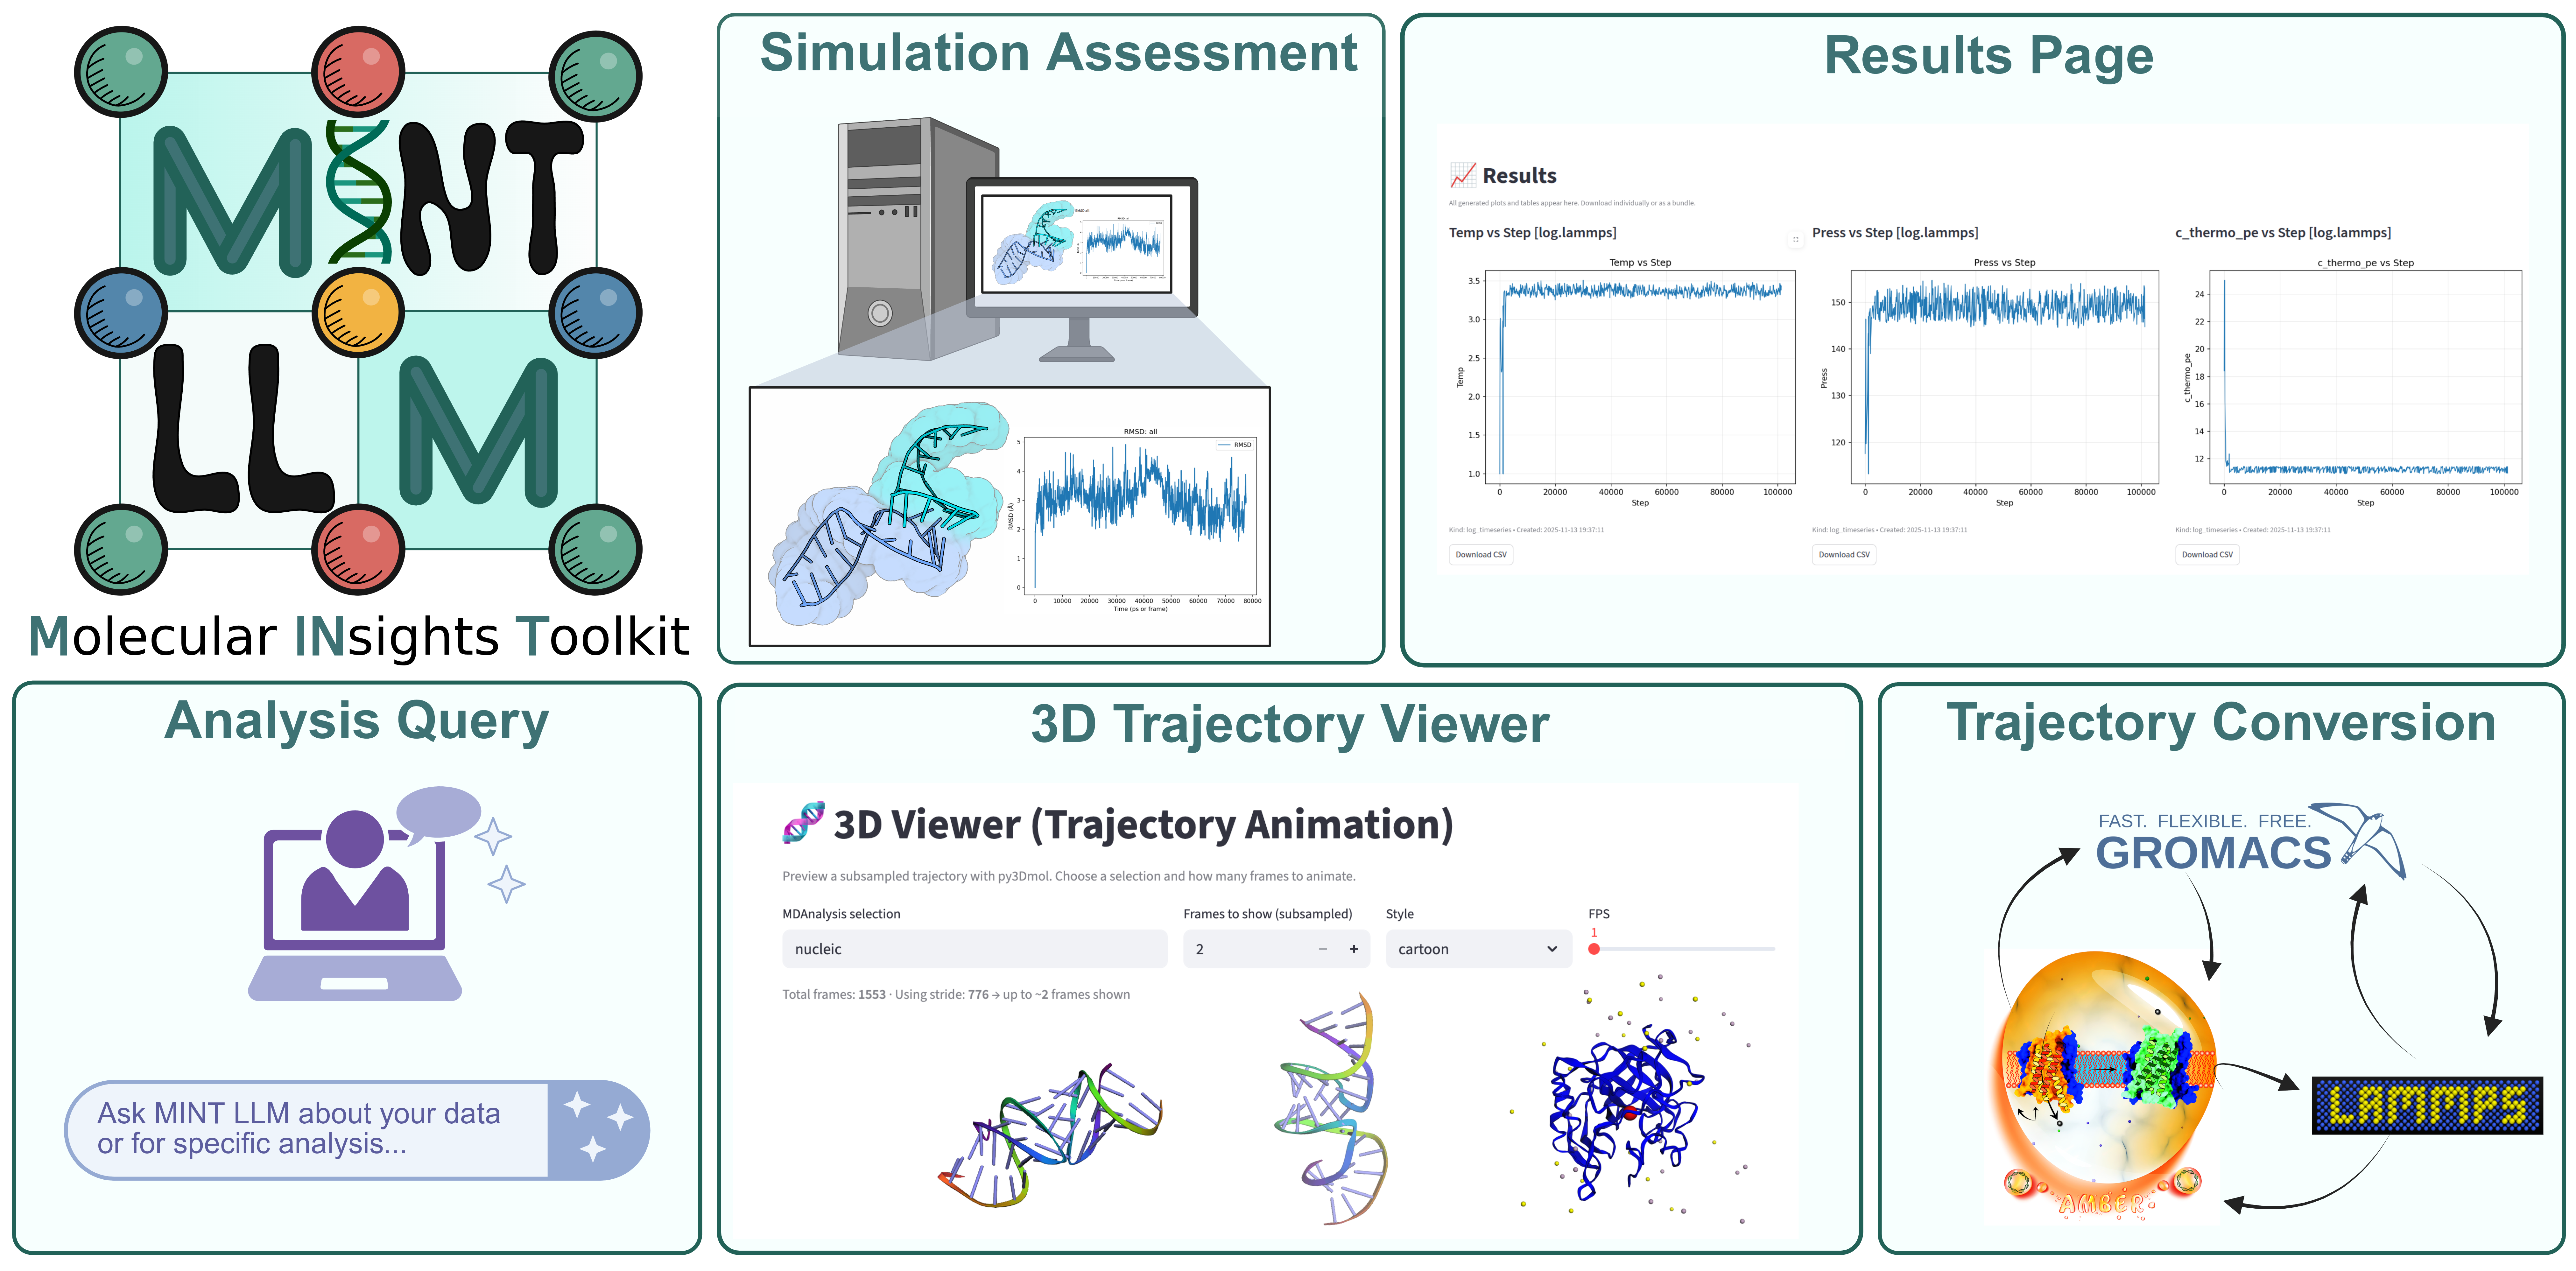
\includegraphics[width=.8\linewidth]{figures/MintLLM.png}
  \caption{Overview of the MINT LLM web application, showing its five core modules: Simulation Assessment, Trajectory Upload, Analysis Query, Results, and Trajectory Conversion. [Created with Biorender.com]}
  \label{fig:MintLLM}
\end{figure}

Under the Simulation Assessment page, users can upload log files from any supported MD engine, including Large-scale Atomic/Molecular Massively Parallel Simulator (LAMMPS) \cite{thompson2022lammps},  GROningen MAchine for Chemical Simulations (GROMACS) \cite{berendsen1995gromacs}, and Assisted Model Building with Energy Refinement (AMBER) \cite{Amber2025}, and MINT LLM automatically generates time-series plots for all relevant variables. For example, uploading a LAMMPS log file produces plots such as Temperature vs. Step, Pressure vs. Step, and Potential Energy vs. Step. All plots generated in this module are automatically stored under the Results page, where users can download individual CSV files or a ZIP archive containing all associated datasets and images.

Users can upload topology and trajectory files through the Trajectory Upload page and initialize them by selecting “Create/Refresh Universe.” Successfully uploaded files are listed below and can be cleared or replaced as needed. The left-hand panel includes an option to upload an OpenAI API key. \cite{OpenAI_API}. If a user uploads a valid API key, the Analysis Query tab will allow users to chat with GPT-5 where users can ask questions about the data, as well as asking the built-in agent to analyze and plot the data for them. For example, if given the query “plot root mean square deviation of the whole structure over time”, the chatbot will give general information about plotting RMSD and then will notify the user that the plot has been completed and users can view plots created by the chatbot in the Results tab with a message such as “Ran RMSD all and added the plot to Results”. Users can also view their trajectories in the 3D viewer tab. The Trajectory Conversion tab allows users to convert the uploaded trajectories to one of the other supported MD engine trajectory formats.


\section*{Future Work}
Future development of MINT LLM will focus on implementing complete functionality in the trajectory conversion module and refining other components of the framework. At present, MINT LLM supports trajectory and log file inputs from AMBER, GROMACS, and LAMMPS simulations. In upcoming versions, we aim to expand compatibility to additional molecular dynamics engines, including oxDNA \cite{poppleton2021oxdna}, HOOMD-blue \cite{anderson2020hoomd}, and others.

\section*{Open-source Materials}

All source code and related materials are available on GitHub and project website.
\github{https://github.com/ncsu-llm-hackathon-materials-2025/MINT-LLM.git}.

\url{https://mint-llm.streamlit.app/}.

\section*{Author Contributions}
C.J.B.: Conceptualization, Software, Visualization, Writing - Original Draft \& Editing; M.F.:  Conceptualization, Software, Visualization, Writing - Original Draft \& Editing, N.J.: Conceptualization, Software, Writing - Review \& Editing; L.B.:  Conceptualization, Software, Writing - Original Draft; D.I.: Software, Writing - Review \& Editing; R.V:  Conceptualization, Software.
\end{teamsubmission}



% %%%%%%%%%%%%%%%%%%%%%%%%%%%%%%%%%%%%%%%%%%%%%%%%%%%%%%%%%
% Team: OntoMapper  %
% %%%%%%%%%%%%%%%%%%%%%%%%%%%%%%%%%%%%%%%%%%%%%%%%%%%%%%%%%

\begin{teamsubmission}{OntoMapper}{Ontology‑Aware Data Mapping with LLM‑Driven Tree Search}
\authorsblock{ 
    Jörg Schaarschmidt\textsuperscript{1}\orcidlink{0000-0002-4389-2366},
    Shankha Nag\textsuperscript{2}\orcidlink{0000-0001-9309-8366},
    Thomas Frank\textsuperscript{1},
    Ebrahim Norouzi\textsuperscript{3},\orcidlink{0000-0002-2691-6995}
    Kostiantyn Hubaiev\textsuperscript{3},
    Wolfgang Wenzel\textsuperscript{1}\orcidlink{0000-0001-9487-4689},
}

\affiliationsblock{
    \textsuperscript{1}Institute of Nanotechnology, Karlsruhe Institute of Technology, Karlsruhe, Germany\
    \textsuperscript{2}Bundesanstalt für Materialforschung‑ und Prüfung (BAM), Berlin\
    \textsuperscript{3}FIZ Karlsruhe – Leibniz Institute for Information Infrastructure, Eggenstein‑Leopoldshafen
}

\section*{Introduction}
In order to provide access to data across distributed resources with different local labels, the data need to be annotated using a semantic approach. This is realized using ontologies, which provide an explicit, formal specification of a shared conceptualization, thereby enabling semantic interoperability across heterogeneous data sources. In many materials‑science collaborations, researchers lack ontology expertise, making it difficult to annotate data for cross‑dataset search and reuse \cite{Bayerlein2025, Schilling2025}. Searching and editing ontologies requires in depth knowledge of their internal structure and special query language. Our OntoMapper tool bridges this gap by coupling large‑language‑model (LLM) reasoning with a structured tree‑search over the target ontology.
\section*{Results}

The workflow starts by parsing RDF/Turtle files with rdflib and constructing a NetworkX graph enriched with \texttt{rdfs:label}, \texttt{skos:altLabel}, and \texttt{skos:definition} for each node. 
A bounded-oracle LLM scores candidate nodes on a 1--100 scale, while a depth-penalty discourages overly generic matches, yielding a composite quality score $S(v)=q(v)-p(d(v))$. 
The agent performs a beam-search on this scored tree, expanding only promising branches; typical runs require $O(k\cdot d)$ LLM calls (with $k = 3$, $d = 5$) instead of exhaustive enumeration. 

To locate a term or a related term within an ontology, we rely on node embeddings. Similarity matching in an embedded vector space is orders of magnitude faster than performing graph traversals. It is important to note that we are not seeking exact matches — hence methods such as SPARQL queries are not suitable for this task.

\begin{figure}[!ht]
\centering
\includegraphics[width=\textwidth]{figures/node_embedding.png}
\caption{Node embedding performed on an ontology}
\label{fig:node-embedding_schematic}
\end{figure}

We evaluated two node embedding approaches. The first, direct node embedding, embeds only the description of each individual node. The second, context-enhanced node embedding, incorporates both the node’s description and the descriptions and connectivity of its neighbouring nodes (Fig. \ref{fig:node-embedding_schematic}).

To validate our results, we used the pre-annotated MuLMS text corpus \cite{schrader2023mulms} to extract domain-relevant terms mentioned in steel-related papers. We then used these terms to evaluate the different approaches. The results were somewhat surprising: the direct node embedding approach performed marginally better (Fig. \ref{fig:node-embedding_result}). We attribute this to additional noise likely introduced by the context-enhanced method. However, we expect context-enhanced embeddings to excel when matching higher-level concepts rather than isolated keywords — an avenue that we plan to explore in future work.

\begin{figure}
\centering
\includegraphics[width=0.5\textwidth]{figures/node_embedding_performance.png}
\caption{Node embedding performed on an ontology}
\label{fig:node-embedding_result}
\end{figure}

\section*{Future Work}
We plan to integrate a hybrid pre‑pruning stage that leverages vector‑based lexical similarity to further reduce LLM query count, and to evaluate the approach on larger, domain‑specific ontologies such as the PMD core ontology \cite{Bayerlein2024}.

\section*{Open‑source Materials}
All code, demonstration notebooks, and the MCP‑compatible service for subtree retrieval are released under BSD3 license at \url{https://github.com/materialdigital/ontomapper}.

\section*{Author Contributions}
W.W.: Conceptualization, Project administration, Writing – review \& editing; J.S.: Conceptualization, Methodology, Software, Writing – original draft, Writing – review \& editing; S.Nag: Methodology, Software, Validation, Visualization, Writing – review \& editing; T.Frank: Data Curation, Visualization, Resources, Writing – review \& editing; E.N.: Resources, Methodology, Formal analysis; K.H.: Resources, Methodology, Formal analysis

\end{teamsubmission}



% %%%%%%%%%%%%%%%%%%%%%%%%%%%%%%%%%%%%%%%%%%%%%%%%%%%%%%%%%
% Team: AtomBridge %
% %%%%%%%%%%%%%%%%%%%%%%%%%%%%%%%%%%%%%%%%%%%%%%%%%%%%%%%%%

\begin{teamsubmission}{AtomBridge}{Extracting crystallographic information for structure generation from S/TEM literature}
\authorsblock{
    Jennifer Garland\textsuperscript{1,2}\orcidlink{0000-0003-2842-5951},
    Gabriel Graves\textsuperscript{3},
    Hyewon Jeong\textsuperscript{4}\orcidlink{0009-0003-1558-1848},
    Ritesh Kumar\textsuperscript{5}\orcidlink{0000-0001-6345-6791}
    Daniel Palmer\textsuperscript{3}\orcidlink{0000-0002-2504-4195},
    Tawfiqur Rakib\textsuperscript{6}\orcidlink{0000-0001-6903-6667},
}
\affiliationsblock{
    \textsuperscript{1} Applied Physics Program, Northwestern University, Evanston, IL, 60208 USA\\
    \textsuperscript{2} Materials Science Division, Argonne National Laboratory, Lemont, IL, 60439 USA \\
    \textsuperscript{3} Independent Researcher, USA\\
    \textsuperscript{4} Department of Materials Science \& Engineering, University of Illinois at Urbana-Champaign, IL 61820 USA\\
    \textsuperscript{5} Pritzker School of Molecular Engineering, The University of Chicago, Chicago, IL 60637 USA\\
    \textsuperscript{6} Department of Mechanical Science \& Engineering, University of Illinois at Urbana-Champaign, IL 61820 USA\\
}

\section*{Introduction}
Experimental electron microscopy (EM) now routinely produces atomic-resolution scanning transmission electron microscopy or transmission electron microscopy (S/TEM) images at scale, offering a direct yet underutilized route from experiments to atomistic simulations. While toolkits such as AtomAI \cite{ghosh2022bridging, ziatdinov2021atomai} and related atom-vision frameworks have enabled large-scale, automated extraction of atom positions from S/TEM images, converting these micrographs into crystallographic information files (CIFs)—especially in the absence of raw data—remains challenging and labor-intensive. \texttt{AtomBridge} addresses this gap by providing an end-to-end, reproducible workflow that integrates robust column localization, symmetry detection, and textual descriptions found in manuscripts using large language models (LLMs), along with geometry and physics-based validation, facilitating reliable CIF generation and atomic simulation environment (ASE)-compatible exports. By automating this process, \texttt{AtomBridge} reduces manual intervention, enhances reproducibility, and accelerates the creation of simulation-ready, experimentally validated datasets for high-throughput computational materials discovery \cite{eliasson2024localization}.

\section*{Results}
\texttt{AtomBridge} integrates literature and image-driven crystallography approaches into a single, auditable Streamlit interface. Its PDF path allows user uploads or selections from a curated library, with PyPDFLoader processing sectioned text and images. The application features auto-suggested prompts derived from abstracts for batch execution over targets, alongside support for ad-hoc custom queries. Following this, an ASE-aware RAG pipeline retrieves relevant ASE snippets from a ChromaDB index (all-MiniLM-L6-v2; top-$k=15$) to anchor Gemini-2.5-Pro code generation. This process constructs \texttt{ase.Atoms} objects and writes CIFs. The generated code runs in an isolated subprocess, utilizing an iterative auto-fix routine (up to three LLM-guided retries). Final outputs undergo multi-tier validation: interatomic-overlap checks ($\leq$ 0.5{\AA}; per-file distance summaries), optional M3GNET relaxation for stability estimation, and CIF-to-CIF geometry comparison against references ($\pm$ 15\% lattice, $\pm 5^\circ$ angles).

The image path in \texttt{AtomBridge} automatically identifies figures from PDFs, correlates subpanels with captions, and permits manual editing or LLM-augmented (Gemini-2.5-Flash) picking of TEM/HAADF-STEM images. After the user manually selects an area of interest and inputs the \mbox{pixel-to-\si{nm}} conversion factor, the pipeline applies CLAHE and a peak search to identify atomic columns. It then computes two non-collinear lattice vectors via DBSCAN clustering of nearest-neighbor shifts, using an FFT fallback to identify reciprocal-space peaks and transform to Crystallography CBF format $(a,b,\gamma)$. These CIF lattice parameters are injected to create generation tasks. The corresponding validation CIFs are immediately displayed and tested in conjunction with the purely-text-derived structures. This end-to-end PDF-to-CIF cycle completes within minutes, having successfully reconstructed micrographs of layered oxides (e.g., LCO) \cite{LCO}, 2D crystals with point defects (e.g., WSe\textsubscript{2}) \cite{WSe2_2D}, and structures with dimensions consistent with existing literature standards. Despite successes with LCO and defects in 2D crystals, the workflow failed to reproduce reasonable .CIF files for more complicated structures, such as semiconducting nanoclusters.

\begin{figure}[H]
    \centering
    \includegraphics[width=0.8\linewidth]{figures/AtomBridge_fig.png}
    \caption{(A) Schematic illustration of \texttt{AtomBridge} workflow. (B) \texttt{AtomBridge} allows users to select the region of interest (ROI) in electron microscopy (EM) images (top) and detects lattice vectors from selected EM images (bottom). (C) \texttt{AtomBridge} is tested for materials with multi-dimesions. (D) \texttt{AtomBridge} extracts structural information in CIF form from journals \cite{LCO, STO_NT} and is equipped with an internal structure validation function. The resulting simulated atomic structures of (E) WSe\textsubscript{2} showing from pristine (top) to vacancies (bottom) \cite{WSe2_2D} and (G) layered LCO that are relaxed by DFT. (B) is reproduced from journals \cite{LCO, STO_NT}  with permission. Copyright 2025 American Chemical Society (left), Copyright 2016 American Chemical Society (right), respectively.}
    \label{fig:AtomBridge_fig}
   
\end{figure}

\section*{Future Work}
Given the difficulties in extracting real-space information from low-quality images in manuscripts, we would like to develop a more robust workflow for extracting both real-space and reciprocal-space information from images. Additionally, we would like to add further stability checks to the generated structures using density functional theory, and a more robust pipeline for foundational machine learning interatomic potentials \cite{batatia2023foundation}.

\section*{Open-source Materials}
Code available on GitHub: \github{https://github.com/dpalmer-anl/AtomBridge.git}

\section*{Author Contributions}
%JG: , GG: , HJ: Conceived the idea and designed the workflow, experiments, extracted, and validated electron microscopy images and lattice vectors, RK: , DP: Developed RAG for ASE code,  generation and Presented Demo , TR: .
JG: Provided initial test materials and TEM image datasets for validation, extracted figures, detected atoms, and calculated lattice vectors from images. GG: Co-developed the LangGraph pipeline, figure extraction with subfigure segmentation, integrated lattice analysis with FFT fallback, implemented structure validation (atom overlap and M3GNET), prompt engineering with auto-suggestion and constraint injection, and built the Streamlit UI with CIF comparison. HJ: Conceived the idea and designed the workflow, experiments, extracted and validated electron microscopy images and lattice vectors. RK: Developed real-space atomic spacing measurement algorithms for lattice vector extraction from STEM images, created UI. DP: Co-developed the LangGraph pipeline, developed RAG for ASE code generation with iterative auto-fix, and presented demo. TR: Implemented DFT and LAMMPS validation for structural stability assessment.
\end{teamsubmission}



% %%%%%%%%%%%%%%%%%%%%%%%%%%%%%%%%%%%%%%%%%%%%%%%%%%%%%%%%%
% Team: GAINS  %
% %%%%%%%%%%%%%%%%%%%%%%%%%%%%%%%%%%%%%%%%%%%%%%%%%%%%%%%%%

\begin{teamsubmission}{GAINS}{GAINS: Generative AI for No-PAIN Structures}
\authorsblock{
    Jos\'e Manuel N\'apoles-Duarte\textsuperscript{1}\orcidlink{0000-0001-6823-4733}
}
\affiliationsblock{
    \textsuperscript{1}Laboratorio de Qu\'imica Computacional, Facultad de Ciencias Qu\'imicas, Universidad Aut\'onoma de Chihuahua, Circuito Universitario s/n, Campus II, C. P. 31125, Chihuahua, Chih., M\'exico
}

\section*{Introduction}
Pan-assay interference compounds (PAINS) are substructures that frequently generate spurious signals in biological assays, leading to false positives and misallocation of experimental efforts \cite{Baell2010,Baell2014}. Classical mitigation relies on rule-based filtering of SMARTS patterns and manual medicinal chemistry.
A key idea is to use LLM generative models to enable structure-aware edits subject to property constraints, offering a complementary path: \emph{repair} problematic motifs rather than discard entire scaffolds.
In this sense, we define \textbf{GAINS} (\emph{Generative AI for No-PAIN Structures}) as a reproducible pipeline that (i) detects PAINS motifs using RDKit filter catalogs, (ii) proposes \emph{minimal} structural edits via a large language model (LLM), and (iii) validates the resulting molecules with cheminformatics descriptors and a synthetic accessibility score (PAINS status, QED, MW, logP, TPSA, HBD/HBA, ROT, SA). 

\section*{Results}
From an initial dataset of 2,000 ChEMBL-derived molecules (filtered to molecular weights below 400~Da), a total of 100 compounds were identified as containing PAINS-related substructures using the RDKit FilterCatalog (PAINS A/B/C). These flagged molecules, served as the input set for the GAINS pipeline.

The generative stage, executed with the \texttt{gpt-5-mini-2025-08-07} model, produced 448 valid molecular candidates. Among these, 373 molecules (83.3\%) successfully removed all PAINS alerts (\texttt{False}), while the remaining 75 (16.7\%) retained partial or modified PAINS motifs (\texttt{True}). This distribution confirms that the majority of GAINS-curated molecules effectively overcame assay-interfering structural patterns while maintaining overall scaffold integrity.


The analysis of molecular transformations proposed by the GAINS pipeline (Figure~\ref{fig:figGAINS} a) revealed a consistent tendency toward \emph{minimal structural repair} rather than full redesign. The most frequent modifications (approximately 70\%) correspond to minor atomic substitutions, in which the global molecular scaffold is preserved while local reactive moieties are subtly altered. This pattern indicates that the LLM effectively internalized a minimal-edit chemical strategy, focusing on structural conservation and local correction of problematic motifs such as styrenes, catechols, or anilines.

Quantitatively, repaired compounds exhibited an average increase in QED of +0.10, a moderate rise in logP (+0.14), and a decrease in polar surface area ($\Delta$TPSA $\approx$ --11~\AA$^2$), suggesting an overall improvement in drug-likeness and physicochemical balance. A detailed breakdown of the most common transformations and their average effects is presented in Table~\ref{tab:transformations}, while the global distribution of original and repaired compounds in the molecular embedding space is shown in (Figure~\ref{fig:figGAINS} b).

As shown in Table~\ref{tab:transformations}, minor atomic substitutions were dominant, improving both QED and logP while moderately reducing TPSA. Chain extensions or substituent additions tended to increase hydrophobicity (logP) but maintained acceptable polarity levels. In contrast, hydroxyl and ether insertions increased TPSA by approximately 10~\AA$^2$, enhancing solubility. Carbonyl additions produced the strongest polarity shifts ($\Delta$TPSA $\approx$ +20~\AA$^2$), whereas scaffold simplifications achieved the highest QED gains (+0.17) by reducing redundant or highly polar fragments.

The UMAP projection (Figure~\ref{fig:figGAINS} b) provides a visual overview of this effect: PAINS-flagged compounds (red triangles) cluster in high-density regions characterized by lower QED values, while the GAINS-repaired structures (colored circles) occupy nearby zones in the latent chemical space, yet shift toward regions associated with higher drug-likeness. 

Altogether, GAINS  is a chemically conservative workflow, capable of selectively editing assay-interfering structures while maintaining key pharmacophoric features. This behavior aligns with the intended goal of structural repair rather than de novo generation, providing a realistic and interpretable route for transforming PAINS-containing molecules into more drug-like analogs suitable for downstream optimization.

\vspace{0.5cm}

\begin{table}[H]
\centering
\caption{Most common structural transformations proposed by the GAINS workflow and their average effects on physicochemical properties.}
\label{tab:transformations}
\begin{tabular}{lcccc}
\toprule
\textbf{Transformation type} & \textbf{Occurrences} & \textbf{$\Delta$QED} & \textbf{$\Delta$logP} & \textbf{$\Delta$TPSA} \\
\midrule
Minor atomic substitution               & 321 & +0.098 & +0.141 & --11.105 \\
Chain extension / substituent added     & 50  & +0.077 & +0.481 & --3.848 \\
Added hydroxyl or ether group           & 23  & +0.017 & --0.304 & +10.735 \\
Simplified scaffold                     & 20  & +0.168 & --0.880 & --13.115 \\
Added carbonyl (=O)                     & 19  & +0.054 & --0.168 & +19.958 \\
\bottomrule
\end{tabular}
\end{table}

\begin{figure}[H]
    \centering
    \includegraphics[width=0.75\linewidth]{figures/figGAINS.png}
    \caption{a) GAINS workflow. b) Two-dimensional UMAP projection of molecular fingerprints showing the distribution of original ChEMBL compounds and LLM-generated structures.
    Red triangles highlight PAINS-flagged motifs, and colored circles represent GPT-repaired candidates (GAINS) according to their quantitative estimate of drug-likeness (QED, color scale).}
    \label{fig:figGAINS}
\end{figure}

\section*{Future Work}
Future work will focus on leveraging pretrained molecular language models such as ChemBERTa, ChemGPT, and Tx-Gemma to enhance GAINS through domain-specific fine-tuning and property-conditioned generation \cite{Chemberta,chemgpt,txgemma}.  
\section*{Open-source Materials}
Source code available on GithHub: https://github.com/napoles-uach/GAINS
\section*{Author Contributions:}
J.M.N.-D.: Conceptualization, Methodology, Implementation, Analysis, Visualization, Writing.

\end{teamsubmission}



% %%%%%%%%%%%%%%%%%%%%%%%%%%%%%%%%%%%%%%%%%%%%%%%%%%%%%%%%%
% Team: ChemGraph-IR %
% %%%%%%%%%%%%%%%%%%%%%%%%%%%%%%%%%%%%%%%%%%%%%%%%%%%%%%%%%

\begin{teamsubmission}{ChemGraph-IR}{Computation and Visualization of Infrared Spectroscopy with ChemGraph}
\authorsblock{
    Murat Ke\c{c}eli\textsuperscript{1}\orcidlink{0000-0001-8588-9272},
    Abdullah al Azmi\textsuperscript{2}\orcidlink{0009-0002-7168-6671},
    Kevin Shen\textsuperscript{3}\orcidlink{0000-0001-9715-7474},
    Jeremy Monat\orcidlink{0009-0004-1360-0918},
    Kelly Tallau\orcidlink{0009-0006-9098-3080},
    Karnamohit Ranka\orcidlink{0000-0002-2810-726X},
    Varun Rishi\orcidlink{0000-0003-0317-3815},
    \'{A}lvaro V\'{a}zquez-Mayagoitia\textsuperscript{1}\orcidlink{0000-0002-1415-6300},
    Thang D. Pham\textsuperscript{1}\orcidlink{0000-0002-5232-4619},
    Sandip Giri\orcidlink{0000-0001-9015-5441}
}
\affiliationsblock{
    \textsuperscript{1}Computational Science (CPS) Division, Argonne National Laboratory, Lemont IL 60517, USA\\
    \textsuperscript{2}Islamic University of Technology, Board Bazar, Gazipur, BGD\\
    \textsuperscript{3}NobleAI, San Francisco, California\\
}

\section*{Introduction}
Infrared (IR) spectroscopy is a powerful experimental technique for probing molecular structure and bonding, yet interpreting IR spectra often requires detailed computational analysis to assign vibrational modes and understand underlying atomic motions.
This analysis typically proceeds by (i) optimizing the equilibrium geometry, (ii) computing the Hessian (mass–weighted second derivatives) to obtain harmonic frequencies and normal modes, and (iii) evaluating IR intensities from the square of the dipole–moment derivative with respect to each normal coordinate \cite{wilson1980molecular}. 

ChemGraph\cite{pham2025chemgraph} is an open-source agentic framework that orchestrates end-to-end computational-chemistry workflows from natural-language requests, automating everything from parameter selection to visualization of final results. 
Building on this foundation, ChemGraph-IR provides a specialized pipeline for IR spectroscopy: given a user query and a molecular structure, it performs geometry optimization, vibrational analysis, IR intensity calculations, and generates both spectra and normal-mode animations with consistent file outputs for downstream analysis. 
Together, these capabilities enable users to compute and visualize IR spectra directly from natural language queries, making spectral interpretation faster and more accessible.

Recent foundation models for atomistic simulation, particularly equivariant graph neural network force fields such as MACE and UMA, deliver first-principles-level accuracy at orders-of-magnitude lower cost, allowing routine frequency computations via finite differences of ML forces and rapid exploration of conformers \cite{batatia2023mace,wood2025uma}. 
In parallel, large language models (LLMs) serve as high-level controllers in ChemGraph, translating user intent into reproducible workflows and reducing manual effort in setup, error recovery, and provenance capture.

Dipole moments (and their derivatives) can be obtained at multiple levels of theory: (i) \emph{ab initio} methods provide high fidelity for intensities and selection rules; (ii) modern semiempirical models such as GFN2-xTB offer speedy dipoles suitable for screening and solvent/ensemble studies \cite{GFN2xTB_JCTC_2019}; and (iii) machine-learning models such as MACE4IR\cite{bhatia2025mace4ir} predict dipoles directly alongside energies and forces, enabling fast IR-intensity estimation when coupled with normal modes from ML potentials. 
Examples include PhysNet, which jointly learns energies, forces, dipoles, and partial charges \cite{PhysNet_JCTC_2019}, and AIMNet2, which learns physics-informed charges to reproduce dipole and quadrupole moments across diverse chemical spaces \cite{AIMNet2_PNASplus_2025}.


\section*{Results}
\begin{figure}[htbp]
\centering
\includegraphics[width=0.6\linewidth]{figures/chemgraph-ir.pdf}
\caption{ChemGraph-IR workflow: from a natural-language request to optimized structure, vibrational analysis, IR intensities, spectrum visualization, and normal-mode animation.}
\label{fig:chemgraph-ir}
\end{figure}

During the LLM Hackathon, we implemented and validated the following capabilities:
\begin{itemize}
  \item \textbf{End-to-end IR pipeline:} Automated geometry optimization, harmonic frequency analysis, and IR‐intensity generation, with robust fallbacks (restarts, stale‐file cleanup, and parameter retries) to improve reliability.
  \item \textbf{Calculator backends:} Integration of an ASE calculator based on AIMNet2~\cite{AIMNet2_PNASplus_2025} and dipole‐moment calculations via GFN2‐xTB~\cite{GFN2xTB_JCTC_2019}, enabling fast ML‐accelerated runs and efficient screening.
  \item \textbf{Interactive visualization:} A user interface that renders the IR spectrum (image and peak table), supports mode selection, and previews animated normal‐mode displacements in 3D to aid interpretation.
  \item \textbf{Reproducible file artifacts:} Standardized outputs for downstream analysis, including \texttt{frequencies.csv}, per‐mode \texttt{.traj} files, and a saved spectrum image (\texttt{ir\_spectrum.png}) for reproducible workflows.
  \item \textbf{LLM backends:} Added Groq support end‐to‐end (dependencies, configuration, loader, and supported‐model registry) to improve portability and provider choice.
\end{itemize}

We also added a Jupyter notebook that demonstrates these features end‐to‐end, and set up documentation to build and deploy automatically via a GitHub Actions workflow using MkDocs, ensuring guidance stays current with each repository update.

\section*{Future Work}
We plan to incorporate anharmonic effects through frequency-scaling schemes alongside explicit treatments based on high-dimensional representation of the potential energy surface and solution of the vibrational Schrödinger equation. 
We will also integrate a curated database of experimental IR spectra with solvent and temperature metadata to enable side-by-side comparison, automated peak matching, and rigorous provenance. 
To quantify accuracy and cost–benefit trade-offs, we will benchmark ML-derived normal modes, frequencies, and intensities against the experimental database. 
\section*{Open-source Materials}
ChemGraph source code is available on GitHub: https://github.com/argonne-lcf/ChemGraph.
We also provide a special release for the hackathon here: https://github.com/argonne-lcf/ChemGraph/releases/tag/v2025.09.12

\section*{Author Contributions}
A.A.: Documentation.
K.S.: Defining and testing IR spectrum tool. IR visualization tool.
J.M.: Documentation and presentation.
K.T.: IR visualization example code gathering and presentation. 
K.R.: Added and tested IR spectrum generation functionality using ASE.
V.R.: Added IR spectrum generation functionality using xTB and ASE.
M.K.: Conceptualization, implementation, testing, and writing.
T.D.P: Conceptualization, implementation, testing. 
S.G: Added open-source model, testing.
\end{teamsubmission}

% %%%%%%%%%%%%%%%%%%%%%%%%%%%%%%%%%%%%%%%%%%%%%%%%%%%%%%%%%
% Team: CLUE  %
% %%%%%%%%%%%%%%%%%%%%%%%%%%%%%%%%%%%%%%%%%%%%%%%%%%%%%%%%%

\begin{teamsubmission}{CLUE}{Crystal Learning for Understandable Explanations}
\authorsblock{
    Elena Patyukova\textsuperscript{1}\orcidlink{0000-0003-1641-5107}
}
\affiliationsblock{
    \textsuperscript{1} Scientific computing department, STFC, UKRI, UK\\
}

\section*{Introduction}

In traditional physics and chemistry, explanations and definitions form the scaffolding of scientific progress. They guide model development, enable fair comparison between approaches, and transform results into reusable knowledge. In contrast, black-box machine learning (ML) models lack inherent interpretability. Thus, developing dedicated methods to explain and interpret their decisions is crucial for building trust, enabling evaluation beyond output statistics, and guiding more purposeful model refinement.

There are roughly 4 groups of XAI methods used for post-hoc explanation of black-box models: (1) feature importance methods (e.g., SHAP~\cite{Lundberg2017}); (2) gradient based methods~\cite{Sundararajan2017}; (3) surrogate model methods (e.g., LIME~\cite{Ribeiro2016}); (4) analysis of counterfactuals~\cite{Wellawatte2023, Wellawatte2025} and examples. Here, we focus on counterfactual explanations. 

A \textit{counterfactual} in the context of chemistry is a molecule or compound that is structurally similar to a given sample but is predicted to exhibit an opposite property. Explanations emerge by identifying and reasoning about structural differences between the sample and its counterfactuals, and relating these differences to the predicted property. Traditionally, this interpretive step relies on human expertise, as it requires flexible reasoning and domain knowledge. However, recent studies have shown that large language models (LLMs) such as ChatGPT and Claude can effectively perform this reasoning for molecular systems~\cite{Wellawatte2025}.  
Here, we extend these ideas to the interpretation of structure–property relationships in crystalline materials—a setting that, to our knowledge, has not been explored before.

\section*{Results}
In this hackathon project, we developed a pipeline to generate counterfactual explanations for structure–property relationships in crystalline materials (Figure~\ref{fig:CLUE-pipeline}). The workflow comprises three stages.

\textbf{Stage 1: Property prediction and counterfactual generation.}  
As the black-box model, we used a random forest (RF) classifier from \texttt{scikit-learn}, chosen for its strong baseline performance and simplicity. The target property is metallicity. The model was trained on the JARVIS 3D-DFT dataset~\cite{Choudhary2020} (metal:nonmetal ratio 0.75:0.25), using an 80:20 train–test split. Features included \texttt{matminer}~\cite{Ward2018} composition and structural descriptors combined with SOAP features (computed for the lattice with atom identities removed). The trained model achieved $\mathrm{ACC}=0.92$, $\mathrm{MCC}=0.81$, and $\mathrm{F1}=0.94$. High performance is essential, as meaningful explanations can only be expected when the model captures genuine structure–property relationships.

To generate counterfactuals, we first compiled a list of candidate elements by selecting the five nearest neighbours for each element in the sample on the Pettifor scale~\cite{Pettifor1984}, as chemically similar elements are more likely to substitute each other. All corresponding compounds were downloaded from the Materials Project database, filtered for thermodynamic stability, and predicted using our trained model. Compounds predicted to have the opposite property were retained. Structural similarity between the sample and each candidate was then computed, and the top ten most similar compounds were selected as counterfactuals.

The overall structural similarity metric is defined as $S_{\text{struct}} = w_{\text{comp}} S_{\text{comp}} + w_{\text{soap}} S_{\text{soap}} + w_{\text{vol}} S_{\text{vol}}$, where $S_{\text{comp}}$, $S_{\text{soap}}$, and $S_{\text{vol}}$ measure similarity in composition, local structure, and volume per atom, respectively.  
Compositional distance is computed via the Earth Mover’s Distance (ElMD~\cite{Hargreaves2020}) using Pettifor distances, rescaled and transformed to similarity as $S_{\text{comp}} = \exp(-\tilde{D}_{\text{comp}})$.  
Structural similarity uses SOAP descriptors~\cite{Bartok2013, Himanen2020}, averaged into orbit vectors per symmetry-equivalent atom. These vectors are matched via the Hungarian algorithm with Pettifor-weighted species similarity. To correct for the insensitivity of our SOAP-similarity to uniform cell expansion, a volume-based similarity term is added: $S_{\text{vol}} = \exp\{-|v_1 - v_2|/2\}$.

\textbf{Stage 2: LLM reasoning over counterfactuals.}  
Each structure is described using the Robocrystallographer tool~\cite{Ganose2019}, which produces human-readable structural descriptions. These are combined into a prompt instructing the LLM (ChatGPT-4-mini) to analyze the structure–property relationships and evaluate their consistency with known chemical principles.

\textbf{Stage 3: Explanation synthesis.}  
The LLM generates a structured explanation linking features of the sample and counterfactuals to the predicted property. The output is stored locally for review.  
We tested the pipeline on five structurally complex compounds; the resulting explanations are available on GitHub.

\begin{figure}[h]
    \centering
    \includegraphics[width=1\linewidth]{figures/CLUE-fig1.png}
    \caption{CLUE workflow.  
    (A) Counterfactual generation: property prediction for the sample and identification of counterfactual structures.  
    (B) LLM reasoning: prompt compilation and structural–property analysis.  
    (C) Explanation: model-generated interpretation of structure–property relationships.}
    \label{fig:CLUE-pipeline}
\end{figure}

\section*{Future Work}
Future directions include:  
(1) investigating how different similarity measures affect the selected counterfactuals and resulting explanations;  
(2) developing quantitative metrics to evaluate explanation quality~\cite{Wellawatte2025}; and  
(3) extending from single-sample (local) explanations to dataset-level analyses that assess model reliability and uncover broader structure–property trends beyond accuracy metrics.

\section*{Open-source Materials}
Code is available on GitHub: https://github.com/epatyukova/llm2025-hackathon-CLUE

\section*{Author Contributions}
E.P.: Conceptualization; E.P., ChatGPT-5: Implementation; Visualization.  ChatGPT-4-mini was used for the generation of explanations.

\end{teamsubmission}



% %%%%%%%%%%%%%%%%%%%%%%%%%%%%%%%%%%%%%%%%%%%%%%%%%%%%%%%%%
% Team: NEDD %
% %%%%%%%%%%%%%%%%%%%%%%%%%%%%%%%%%%%%%%%%%%%%%%%%%%%%%%%%%

\begin{teamsubmission}{NEDD}{Next Experiment Data Driven}
\authorsblock{
    Viktoriia Baibakova\textsuperscript{1}\orcidlink{0009-0004-5799-9510}
}
\affiliationsblock{
    \textsuperscript{1}Electrification and Energy Infrastructures Division, Oak Ridge National Laboratory, 1 Bethel Valley Road, Oak Ridge, 37830, TN, USA\\
}

\section*{Introduction}
When experiments are conducted, the parameter space is often sampled non-uniformly, resulting in skewed data distributions and regions of ignorance—areas where no experiments have been performed. Machine learning models perform best when trained on diverse, representative datasets; if experiments are clustered in a narrow region of the parameter space, the model’s ability to generalize is severely limited, leading to biased training and inaccurate predictions. NEDD mitigates this issue by visualizing the parameter space, identifying unexplored regions, and suggesting next experiments using active learning rather than randomness.~\cite{wei2025discovering} Additionally, the integrated LLM assistant enables natural language querying of experimental data and provides informed guidance for future experiments.

\section*{Results}
NEDD (Next Experiment Data-Driven) is implemented as a local server or Streamlit-based user interface, allowing scientists to interact with machine learning–driven experiment planning without writing code. ~\cite{khorasani2022web} Because the system runs locally, all experimental data remain on the user’s machine, preserving confidentiality and enabling secure use in laboratory or industrial environments. 

\begin{figure}[h]
    \centering
    \includegraphics[width=0.92\linewidth]{figures/nedd.png}
    \caption{NEDD user interface for data-driven experiment planning. A) Data upload and tabular view where the rightmost column is interpreted as the target variable. B) Interactive pairplot visualizing parameter distributions and gaps in explored space. C) GPR output showing predictive mean, uncertainty, and top five suggested next experiments using uncertainty sampling and expected improvement. D) Integrated Claude LLM chat interface enabling natural-language queries about data trends, experimental strategies, and model outputs.}
    \label{fig:nedd}
\end{figure}

The workflow begins with users uploading a dataset in tabular format, see Figure~\ref{fig:nedd}. NEDD automatically parses the table, interprets all columns except the rightmost as input features, and treats the rightmost column as the target variable. The platform supports an unlimited number of numerical features (categorical support under development), making it compatible with high-dimensional synthesis or characterization datasets. Within the UI, the dataset is visualized through interactive pairwise parameter plots and kernel-density projections, enabling users to detect data skewness, clustering, and unvisited regions of parameter space. These visual tools are designed specifically for non-coding users, allowing experimentalists to understand dataset structure and coverage without scripting. NEDD automatically trains a Gaussian Process Regression (GPR) model with ARD kernel on the uploaded dataset to estimate predictive mean and uncertainty. ~\cite{khorasani2022web, chhajer2024rationalised} Based on the trained surrogate model, NEDD recommends the top five next experiments using two acquisition strategies. Uncertainty Sampling prioritizes regions with high model uncertainty to improve overall predictive confidence (exploration mode). Expected Improvement (EI) targets conditions likely to exceed current best performance (exploitation mode). The platform provides both modes via UI toggles, enabling users to shift between knowledge expansion and performance optimization. 

A key innovation of NEDD is its integration of a Claude LLM Chat (via API), which enables natural-language interrogation of the dataset and model outputs (e.g., “How can I reduce parameter imbalance?”). ~\cite{claude2024nedd} The LLM does not access the raw data externally; instead, it analyzes metadata, summaries, or computed statistics to provide guidance on trends, biases, and next steps. 

Using data-guided experimental approaches significantly reduces the number of iterations required to reach optimal conditions compared to random or expert-only sampling methods. These strategies leverage prior results or model predictions to select new, informative experimental conditions. This targeted approach results in faster convergence towards optimal or desired outcomes while also requiring fewer trial runs, saving both time and computational resources. ~\cite{chhajer2024rationalised}

I note that I used the CLine AI coding assistant with the Claude LLM to accelerate code development and debugging during implementation. ~\cite{cline2024nedd}

\section*{Future Work}
I plan to extend data-handling capabilities, increase active-learning model robustness, and integrate a local LLM to enable direct, privacy-preserving interaction with data.

\section*{Open-source Materials}
Code is available on GitHub: \github{https://github.com/ViktoriiaBaib/NEDD}

\section*{Author Contributions}
V.B.: Conceptualization, Execution, Visualization.
\end{teamsubmission}



% %%%%%%%%%%%%%%%%%%%%%%%%%%%%%%%%%%%%%%%%%%%%%%%%%%%%%%%%%
% Team: T2-Relax %
% %%%%%%%%%%%%%%%%%%%%%%%%%%%%%%%%%%%%%%%%%%%%%%%%%%%%%%%%%

\begin{teamsubmission}{T2-Relax}{Text to text (T2) crystal relaxation}
\authorsblock{
    Daniel T. Speckhard\textsuperscript{1}\orcidlink{0000-0002-9849-0022},
    Aniket Phutane\textsuperscript{2}\orcidlink{0009-0007-4043-6908},
    Alexander Kister\textsuperscript{3},
    Heike Quosdorf\textsuperscript{3}\orcidlink{0000-0001-8348-7405},
    Claudia Draxl\textsuperscript{1}\orcidlink{0000-0003-3523-6657},
    José A. Márquez\textsuperscript{1}\orcidlink{0000-0002-8173-2566}}
\affiliationsblock{
    \textsuperscript{1}Humboldt-Universit\"at zu Berlin, Zum Gro\ss en Windkanal 2, 12489 Berlin, Germany\\
    \textsuperscript{2}Helmholtz-Zentrum Berlin für Materialien und Energie\\
    \textsuperscript{3}Bundesanstalt für Materialforschung und -pr\"ufung (BAM)\\
}

\section*{Introduction}

Crystal structure relaxation is an integral part of high throughput computational workflows, which often optimize the geometry of thousands of structures, selecting a DFT code and the corresponding computational parameters~\cite{speckhard2025big, speckhard2025workflows}. In this project, we use the LeMatTraj dataset~\cite{ramlaoui2025lemat} to train an LLM (T5-Transformer)~\cite{raffel2020exploring} to perform crystal structure relaxation. In order to feed the model textual input data, we use the ASE library~\cite{larsen2017atomic} to transform the crystal structure into a crystallographic input file (CIF), which is the standard in the Inorganic Crystallographic Database (ICSD)~\cite{hellenbrandt2004inorganic}, and aim at predicting the relaxed structure in the CIF format via $\Delta$-learning~\cite{speckhard2025extrapolation}. This work was largely inspired by the MD-LLM-1 work~\cite{murtada2025md}, which predicted relaxed protein structures using an LLM. To improve the LLM's performance, we fine-tune the model on the relaxation task.

\section*{Results}

The T5-Transformer is an LLM that was trained on the C4 text corpus for natural language processing (NLP) tasks (e.g. translation, summarization, question answering, etc.).  The model is fine-tuned to optimize text-based metrics (ROUGE~\cite{lin2004rouge} and BLEU~\cite{papineni2002bleu}) to ensure that much of the CIF file remains unchanged after relaxation (i.e., the atomic elements in the structure). Using a weighted sum, the model is also fine-tuned to minimize the RMSE of the lattice parameters and atomic positions,  which are givenrelative to the basis vectors. Since the crystal structures in the LeMatTraj dataset have a wide distribution, we apply $\Delta$-learning~\cite{speckhard2025extrapolation} to predict the differences in the lattice parameters (lengths and angles between them) from the initial structures to the final structures as obtained by DFT. In this way, the target distribution is more Gaussian. The general framework of the approach is shown in Figure~\ref{fig:t2_relax_pipeline}.

\begin{figure}[h]
    \centering
    \includegraphics[width=0.92\linewidth]{figures/t2_relax_pipeline.pdf}
    \caption{Overview of the relaxation training pipeline. The input structure from the LeMatTraj dataset is transformed to a CIF file using ASE. It then is fed into the T5 tokenizer and the fine-tuned transformer block layers to output a relaxed structure CIF file.}
    \label{fig:t2_relax_pipeline}
\end{figure}


The results are shown in Table~\ref{tab:t2_relax_parameter_crystal_cell_errors}. The MAE and RMSE of the predicted change in the atomic positions for each structure in the dataset are shown in Table \ref{tab:t2_relax_crystal_positions}. In general, we see small errors, which show that the LLM manages to generally predict the relaxed structured with a good degree of accuracy. Without the ROUGE and BLEU metrics to keep the elements the same from the input to the predicted CIF output, the LLM often removes atoms or changes them. More thorough testing is required to benchmark the method, but the initial results shown here are promising.

\begin{table}[h!]
\centering
\begin{tabular}{|l|c|c|c|}
\hline
\textbf{Parameter} & \textbf{MAE} & \textbf{MSE} & \textbf{RMSE} \\
\hline
$\Delta a$ (\AA) & 0.053 & 0.006 & 0.080 \\
$\Delta b$ (\AA) & 0.053 & 0.006 & 0.080 \\
$\Delta c$ (\AA) & 0.074 & 0.020 & 0.140 \\
$\Delta \alpha$ ($^\circ$) & 0.086 & 0.036 & 0.189 \\
$\Delta \beta$ ($^\circ$) & 0.101 & 0.070 & 0.265 \\
$\Delta \gamma$ ($^\circ$) & 0.160 & 0.104 & 0.322 \\
\hline
\end{tabular}
\caption{Errors in predicting the lattice cell parameters.}
\label{tab:t2_relax_parameter_crystal_cell_errors}
\end{table}

\begin{table}[h!]
\centering
\begin{tabular}{|l|c|}
\hline
\textbf{Metric} & \textbf{Value} \\
\hline
MAE & 0.066 \AA \\
MSE & 0.252 \AA$^2$ \\
RMSE & 0.502 \AA \\
\hline
\end{tabular}
\caption{Errors in predicting the relaxed atom positions}
\label{tab:t2_relax_crystal_positions}
\end{table}

\section*{Future Work}
Future work should seek to use larger LLM models, use a larger combined dataset (e.g., data from NOMAD~\cite{draxl2019nomad}), and perform a systematic comparison with state-of-the art graph neural network methods used in materials science~\cite{rhodes2025orb, bechtel2025band}.

\section*{Open-source Materials}
Code and tutorial video are available on GitHub: \github{https://github.com/anky3733/Traj}.
\section*{Author Contributions}
D.S.: conceptualization, code, writing.
A.P.: conceptualization, code.
A.K.: conceptualization, code, reviewing.
H.Q.: conceptualization, code, reviewing.
C.D.: editing.
J.M.: supplying data, reviewing.

\section*{Acknowledgements}
This work was supported by the NFDI consortium FAIRmat - Deutsche Forschungsgemeinschaft (DFG) - Project 460197019.
\end{teamsubmission}


\begin{teamsubmission}{MaterialSim AI Agent}{An AI-Driven Agent for Automating Computational Materials Simulations}
\authorsblock{
    Awwal Oladipupo\textsuperscript{1}\orcidlink{0009-0006-3979-2078},
    Vallabh Vasudevan\textsuperscript{1}\orcidlink{0000-0001-7933-4924},
    Akhila Ponugoti\ \textsuperscript{2}\orcidlink{0009-0007-8947-7794},
    Toheeb Balogun\textsuperscript{3},
   Jodie A. Yuwono\textsuperscript{4}\orcidlink{0000-0002-0915-0756}
}

\affiliationsblock{
    \textsuperscript{1}Department of Chemical Engineering, University of Michigan\\
    \textsuperscript{2} Johns Hopkins University, USA\\
    \textsuperscript{3}Department of Chemical Engineering, Louisiana State University, USA,
    \textsuperscript{4}Department of Chemical Engineering, University of Adelaide, Adelaide, Australia 
}

\section*{Introduction}
Designing new materials traditionally involves time-consuming, expert-driven processes to configure molecular dynamics (MD) simulations, select interatomic potentials, tune parameters, and analyze results. These manual steps hinder rapid exploration of chemical space. MaterialSim is an open-source Python-based AI agent that integrates large language models (LLMs) with computational materials science tools to automate these workflows. Using natural language instructions, researchers can design, execute, and analyze MD simulations, extract properties like radial distribution functions, mean squared displacements, elastic constants, and thermal conductivity, and leverage machine learning for accelerated predictions. Scalable from laptops to high-performance computing (HPC) clusters and featuring a web-based GUI for interactive 3D visualization, MaterialSim streamlines materials discovery, making it efficient, adaptive, and accessible. By reducing manual effort, it accelerates innovation in materials design and scientific research.

\section*{Results}
MaterialSim is an open-source Python package designed to automate computational materials science tasks by integrating large language models (LLMs) with established tools like LAMMPS \cite{plimpton1995fast} and the Atomic Simulation Environment (ASE) \cite{larsen2017atomic}. It enables researchers to perform molecular dynamics (MD) simulations, calculate material properties (e.g., radial distribution functions, mean squared displacements, elastic constants, thermal conductivity), and apply machine learning (ML) models for predictive analytics using natural language queries. MaterialSim integrates with databases such as Materials Project \cite{Jain2013}, NOMAD \cite{draxl2019nomad}, and Open Catalyst Project \cite{chanussot2021open} for structure retrieval and data augmentation. A Streamlit-based graphical user interface (GUI) provides interactive 2D/3D visualizations, and compatibility with high-performance computing (HPC) clusters via SLURM ensures scalability. By translating queries like ``Simulate the thermal conductivity of silicon at 300 K'' into executable workflows, MaterialSim lowers barriers for researchers, educators, and interdisciplinary teams, accelerating materials discovery.
\begin{figure}[H]
    \centering
    \includegraphics[width=0.60\linewidth]{figures/MaterialSim workflow.pdf}
    \caption{Workflow of MaterialSim AI Agent.}
    \label{fig:materialSim pipeline}
\end{figure}

\section*{Future Work}
Looking ahead, we aim to advance this framework toward a fully integrated, autonomous computational workflow. Our vision is for researchers to initiate simulations, track their progress, analyze outputs, and generate predictive insights through natural-language interaction with an AI system. By enabling complex modelling tasks to be conducted through intuitive dialogue rather than specialized interfaces, this approach has the potential to broaden access to state-of-the-art computational methods and accelerate simulation-driven scientific discovery. 

\section*{Open-source Materials}
Code is available on GitHub: \github{https://github.com/Awwal41/MaterialSim.git}

\section*{Author Contributions}
A.O.: Conceptualization, Resources, Supervision, Methodology, Software, Writing - Original Draft, Writing - Review \& Editing; V.V.: Investigation, Methodology, Data Curation, Writing - Review \& Editing; A.P.: Software, Visualization; T.B.:  Formal Analysis, Writing - Review \& Editing; J.Y: Formal Analysis, Writing - Review \& Editing
\end{teamsubmission}



% %%%%%%%%%%%%%%%%%%%%%%%%%%%%%%%%%%%%%%%%%%%%%%%%%%%%%%%%%
% Team: SCARA %
% %%%%%%%%%%%%%%%%%%%%%%%%%%%%%%%%%%%%%%%%%%%%%%%%%%%%%%%%%

\begin{teamsubmission}{SCARA}{LLM-Hackathon for Applications in Materials Science and Chemistry
Steel Corrosion Agent for Risk Assessment (SCARA)}
\authorsblock{
    Hussein AlAdwan\textsuperscript{1}\orcidlink{0009-0008-9940-7156},
    Mohammed ALI AlKubaish\textsuperscript{1},
    Oswaldo Rodriguez\textsuperscript{1},
    Chahd Rahyl Adjmi\textsuperscript{1},
    Muhammad Ahmed\textsuperscript{1},
    Motasem Ajlouni\textsuperscript{2}
}
\affiliationsblock{
    \textsuperscript{1}King Fahd University of Petroleum and Minerals, SA\\
    \textsuperscript{2}University of Science and Technology of China
}

\section*{Introduction}
Steel is the backbone of industrial infrastructure, from pipelines and refineries to marine and transportation systems. Despite its strength and cost-effectiveness, its durability is constantly threatened by corrosion, especially in aggressive environments such as (\ce{CO2} / \ce{H2S}/ HCl) mixtures. Corrosion weakens structural integrity and contributes to billions of dollars in global annual losses through maintenance, inspection, and premature failures~\cite{SCARA1}.
Conventional corrosion assessment methods based on ASTM/NACE standards, experimental testing, and scattered databases are slow, fragmented, and reactive, limiting timely decision-making in critical industries like oil \& gas and infrastructure~\cite{SCARA2}.
Recent advances in Large Language Models (LLMs) offer a transformative opportunity. By integrating standards, datasets, and literature, LLMs can act as digital corrosion experts, providing rapid predictions, explainable reasoning, and alloy recommendations.
This hackathon project introduces SCARA (Steel Corrosion Agent for Risk Assessment), an LLM powered assistant designed to:
•	Predict corrosion risk under defined conditions.

•	Provide standardized risk scores (low, medium, high).

•	Recommend safer alloys supported by data and standards.
SCARA consolidates scattered corrosion knowledge into a unified, intelligent platform, aiming to enhance reliability, safety, and cost efficiency across industrial applications.

Scara workflow (\ref{fig:SCARA}) is a designed LLM-Based framework to predict the steel performance of industrial and urban environments. The process initiates with the user input, which describes the environment (phase types, composition, thermodynamic conditions, and a brief description of the application (geometry, methodology, and location). The steel standard used, such as AISI, API, or UNS is fed, and the system automatically links the standard to the composition of the steel through the LLM model and the MatWeb materials database extracting the composition of the given designations. The prompt information is submitted to the LLM-Agent trained in scientific papers, review papers, books, and risk assessment standards
The agent analyzes the data provided and generates supporting evidence, estimates the corrosion risk, and recommends possible steel suggestions. A validator checks the consistency of the predictions within a defined risk scale, if the validation converges the results are approved and the final risk assessment is report with the validated evidence while the inconsistent outputs are recalculated. SCARA integrates in this form the documentation, material data and LLM-agent reasoning to deliver evidence-based corrosion evaluations. 

\section*{Results}
Figure \ref{fig:SCARresults} demonstrates the performance of SCARA-Agent against two different predictive methodologies, namely, OpenAI’s common model (prompted by the same text) and the supervised ML algorithms. SCARA-Agent outperforms the open AI model with a 15\% gap, however, the more specialized supervised approach proved a better performance, which is justifiable considering that SCARA-Agent is still a demo version of what can be a general corrosion scientist agent. 
SCARA demonstrates the potential of LLM Agents to evaluate corrosion risk by integrating standards, literature, and material databases into a decision-making platform. Unlike conventional approaches that are often fragmented scope-limited, SCARA provides rapid corrosion predictions, flexible risk assessment, and alloy recommendations backed by scientific evidence.


\begin{figure}[h]
    \centering
    \includegraphics[width=0.65\linewidth]{figures/SCARA.png}
    \caption{SCARA (Steel Corrosion Agent for Risk Assessment) general workflow.}
    \label{fig:SCARA}
\end{figure}
\begin{figure}[h]
    \centering
    \includegraphics[width=0.65\linewidth]{figures/SCARresults.png}
    \caption{SCARA (Steel Corrosion Agent for Risk Assessment) general workflow.}
    \label{fig:SCARresults}
\end{figure}
\section*{Future Work}
Although still in its demo phase, SCARA outperforms general-purpose AI models and shows promise as a scalable digital corrosion expert. While specialized supervised ML methods currently deliver higher accuracy, SCARA’s strength lies in its adaptability, explainability, and integration of domain-specific knowledge. With further refinement, SCARA could evolve into a reliable and practical tool to enhance safety, reduce costs, and improve materials selection across critical industrial sectors.

\section*{Open-source Materials}
Code available on GitHub: \github{https://github.com/https://github.com/mo-alkubaish/SCARA}

\section*{Author Contributions}
H.A.: Conceptualisation, Data Curation, Analysis, Software, Writing,; M.A.: Software, Data Curation; O.R.: Conceptualisation, Data Curation, Writing, Visualisation; C.A.: Data Curation, Visualisation; M.A.; Data Curation, M.A.: Software.
\end{teamsubmission}



\begin{teamsubmission}{Team ChromatographyMiner}{ChromatographyMiner: Interactive Platform for Gas Chromatography Data Analysis with AI-Assisted Interpretation}

\authorsblock{
    Md Habibur Rahman\textsuperscript{}\orcidlink{0000-0002-7705-984X}}

\affiliationsblock{
    \textsuperscript{} School of Materials Engineering, Purdue University, West Lafayette, IN 47907, USA}


% =====================================================================
\vspace{1.5em} % Add some vertical space before the main title
% =====================================================================



\vspace{-0.75em}
%\begin{tcolorbox}[colback=codebg,colframe=myblue,title=\textbf{Introduction}]

\section*{Introduction}
This report describes \texttt{ChromatographyMiner}, an interactive web-based platform that simplifies the analysis of gas chromatography–mass spectrometry and two-dimensional gas chromatography–mass spectrometry data. The system works with files from any instrument manufacturer and supports several input types, including raw data files, two-dimensional chromatogram images, and one-dimensional mass spectra in either spreadsheet or image formats. A major feature of the platform is its flexible and reliable spectral library management. It can automatically download reference data from the MassBank library, load local databases such as MassBank and MassBank of North America, and also accept user-uploaded spectral library files. To identify chemical compounds efficiently, \texttt{ChromatographyMiner} uses a fast matching algorithm that quickly narrows down possible candidates from very large libraries. Each candidate is then ranked based on both the similarity of its mass spectrum and the difference in its retention time. In addition, an artificial intelligence module can generate a clear, structured explanation for the top-ranked match, helping users understand why a compound was identified. Finally, users can curate and save their results as a downloadable PeakCard, which provides a complete and traceable record of the analysis.
%\end{tcolorbox}

\begin{figure}[H]
  \centering
  \includegraphics[width=0.98\textwidth]{figures/ChromatographyMiner.png}
  \caption{User interface of \texttt{ChromatographyMiner}, showing the process of uploading and analyzing two-dimensional gas chromatography–mass spectrometry (GC×GC–MS) data in NetCDF format. The platform allows users to drag and drop .CDF files, visualize the chromatogram, automatically extract mass spectra, and identify top candidate compounds from spectral libraries such as MassBank and MassBank of North America.}
  \label{fig:ChromatographyMiner}
\end{figure}

\section*{Results}
The developed platform provides a fast, flexible, and vendor-neutral solution for identifying chemical compounds from gas chromatography–mass spectrometry and two-dimensional gas chromatography–mass spectrometry data. By combining efficient top-ion pre-filtering with large-scale public spectral libraries such as MassBank and MassBank of North America, it achieves rapid and high-quality tentative compound identifications as shown in \textbf{Figure \ref{fig:ChromatographyMiner}}. \\

The system’s curated output file, \texttt{saved\_refs.json}, links observed chromatographic peaks to definitive reference spectra from the libraries, ensuring traceability and reproducibility across different experiments. Benchmark results show:
\begin{itemize}
    \item \textbf{Speed:} Up to 30 times faster than conventional full-spectrum cosine-matching workflows on libraries containing more than 50,000 spectra.
    \item \textbf{Accuracy:} Correct compound retrieval for approximately 90\% of benchmark peaks from the MassBank dataset (top five ranking).
    \item \textbf{Scalability:} Capable of processing MassBank of North America archives larger than 5 gigabytes using the streaming mass spectral parser without memory limitations.
\end{itemize}



\section*{Future Work}

Future development will focus on expanding compatibility to additional vendor-neutral formats such as the mzML standard, implementing automated co-elution deconvolution algorithms, and integrating external chemical databases such as PubChem and ChemSpider to enrich the final identification records with chemical properties and metadata. Upcoming updates will also include a dedicated Python software development kit (SDK) and web-based application programming interface (API) for high-throughput, programmatic analysis. 

\section*{Open-source Materials}
All code, documentation, and example datasets are publicly available under the MIT open-source license at:  
\github{https://github.com/msehabibur/gcxgc_peakcards}



\section*{Author Contributions}
\textbf{M.H.R} Conceptualization, software development, data processing, validation, and manuscript preparation.  

\end{teamsubmission}



% %%%%%%%%%%%%%%%%%%%%%%%%%%%%%%%%%%%%%%%%%%%%%%%%%%%%%%%%%
% Team: datalab %
% %%%%%%%%%%%%%%%%%%%%%%%%%%%%%%%%%%%%%%%%%%%%%%%%%%%%%%%%%

\begin{teamsubmission}{datalab}{\texttt{guillemot}: automated Rietveld refinement using agents}
\authorsblock{
    Joshua Bocarsly\textsuperscript{1}\orcidlink{0000-0002-7523-152X},
    Benjamin Charmes\textsuperscript{2}\orcidlink{0009-0007-9474-8632},
    Matthew L. Evans\textsuperscript{2,3,4,5}\orcidlink{0000-0002-1182-9098}
    Benjamin Smith\textsuperscript{2}\orcidlink{0000-0001-9673-2449}
    Yue Wu\textsuperscript{6}\orcidlink{0000-0003-2874-8267}
}
\affiliationsblock{
    \textsuperscript{1}Department of Chemistry, University of Houston\\
    \textsuperscript{2}datalab industries ltd., King's Lynn, UK\\
    \textsuperscript{3}MODL-IMCN, UCLouvain, Belgium\\
    \textsuperscript{4}Matgenix SRL, Belgium\\
    \textsuperscript{5}Yusuf Hamied Department of Chemistry, University of Cambridge\\
    \textsuperscript{6}Independent Researcher
}

\section*{Introduction}


In this project, we asked whether a multimodal LLM agent could be used to automate a traditionally human-intensive data fitting task: pattern fitting of powder X-ray diffraction data. A major bottleneck in materials discovery lies in analysing the growing volume of characterisation data produced by high-throughput experiments. Current AI methods  typically rely on ensemble models trained on synthetic data or automated refinements that select the best fit from user-supplied phases \cite{Szymanski2021, Szymanski2023, Chang2025}. These approaches contrast with traditional Rietveld refinement, where experts iteratively improve fits through visual inspection rather than solely paying attention to quantitative metrics. The best Rietveld analysis frequently requires a degree of judgement to avoid overfitting or reporting non-physical results. We hypothesized that multimodal LLM's ability to interpret visual data and incorporate chemical knowledge could enable automated systems that emulate this expert-driven workflow. By empowering an AI agent to perform refinements and interpret the visual and textual output directly, any type of structural modelling (within the broad confines of the refinement software) can be investigated. This offers a key advantage over pre-trained models, which are limited to the scope of structures represented in their training data.

\section*{Results}

\begin{figure}[ht]
  \centering
  \includegraphics[width=0.58\textwidth]{figures/Guillemot.png}
  \caption{A flowchart representing the \texttt{Guillemot} workflow cycle. The AI agent can interact with the user, structural databases and TOPAS to automate a more natural human workflow for Rietveld refinements.}
  \label{fig:Guillemot}
\end{figure}

A provider-agnostic LLM-powered agent, \texttt{Guillemot} \github{https://github.com/datalab-org/guillemot}, was created using the Pydantic AI framework and provided with several tools. Upon receiving a diffraction pattern (optionally downloaded from a \emph{datalab} instance \cite{Evans2025a}) and rubric from the researcher, for example "I have made a sample containing Mn and Sb", \texttt{Guillemot} will first perform a unified query of the federation of $\sim$20 open crystal structure databases comprising the OPTIMADE consortium \cite{Evans2024a, Evans2021} for relevant crystal structures, prioritising those with prior experimental grounding. \texttt{Guillemot} then makes a judgement as to which trial phases to include in an initial refinement. From these phases, it can create a TOPAS \cite{Coelho2018} input file, execute a Rietveld refinement of the trial phases and then process the output into a graphical summary. \texttt{Guillemot} also is able to use a tool to replot the information and zoom into selected regions of interest, such as the dominant or impurity peaks, just as a human expert might. The agent will then assess the quality of the refinement and decide on the next steps, i.e., pick another phase from the trial set, attempt to model impurities via inclusion of additional phases, or add strain to the trial crystal structure, as well as any of the other functionality exposed via TOPAS.

Without needing any fine-tuning, frontier models were capable of writing TOPAS input files with only a few examples, making adjustments based on any formatting or syntax errors emitted by TOPAS.


\section*{Future Work}

This project focused on a specific analyis task: Rietveld refinement using the TOPAS Academic software, which is a commonly used proprietary software for advanced analysis. In the future, it would be valuable to extend this methodology to empower the agent to use of other software, including open-sourced Rietveld refinement software such as GSAS or Profex/BGMN, as well as software that is used by researchers for fitting other types of data. Additionally, we plan to integrate \texttt{Guillemot} with research data management platforms, such as \emph{datalab}, that store PXRD data, allowing analysis to be performed in the background. We also believe \texttt{Guillemot}’s performance and robustness could be improved with model fine-tuning or improved prompting with TOPAS documentation and other information on powder diffraction. Another failure mode was incorrect understanding of refinement output graphs. Further investigation of vision-language models’ (VLM) ability to parse scientific plots would be valuable, to determine how to specifically engineer specific output graph formats suited to VLM analysis.

\section*{Open-source Materials}

Code is available on GitHub under the terms of the MIT license at \github{https://github.com/datalab-org/guillemot} \texttt{datalab-org/guillemot}.

\section*{Author Contributions}
J.B.: Conceptualization, Software, Data Curation, Writing.
B.C.: Software, Data Curation.
M.L.E.: Conceptualization, Software, Data Curation, Writing.
B.S.: Conceptualization, Software, Data Curation, Writing.
Y.W.: Conceptualization, Software, Data Curation, Writing.

\end{teamsubmission}



% %%%%%%%%%%%%%%%%%%%%%%%%%%%%%%%%%%%%%%%%%%%%%%%%%%%%%%%%%
% Team: XAScribe %
% %%%%%%%%%%%%%%%%%%%%%%%%%%%%%%%%%%%%%%%%%%%%%%%%%%%%%%%%%

\begin{teamsubmission}{XAScribe}{XAScribe: An AI-Powered Platform for Automated, Manuscript-Ready X-ray Absorption Spectroscopy Analysis}
\authorsblock{
    Yuanlong Bill Zheng\textsuperscript{1},
    Matthew Miyagishima\textsuperscript{1},
    Rahul Mallela\textsuperscript{1},
    Tim Greitemeier\textsuperscript{1}\orcidlink{0009-0005-2004-3088},
    Shakul Pathak\textsuperscript{2}\orcidlink{0009-0006-3244-1670},
    Yiming Chen\textsuperscript{3}\orcidlink{0000-0002-1501-5550}
}
\affiliationsblock{
    \textsuperscript{1} Pritzker School of Molecular Engineering, University of Chicago, IL, USA \\
    \textsuperscript{2} Department of Chemical Engineering, Massachusetts Institute of Technology, Cambridge, MA, USA \\ 
    \textsuperscript{3} Argonne National Laboratory, Lemont, IL, USA \\
}

\section*{Introduction}
X-ray Absorption Spectroscopy (XAS) is a technique that measures absorption of X-rays over a range of energies. This can reveal the oxidation state and coordination environment of atoms in materials \cite{bunker2010xafs}. This technique has been found to be important in Nickel Cobal Manganese Oxide (NCM) battery cathode materials where the oxidation state and coordination environment of Ni change over cycling \cite{yan2020nmcxas}. While XAS data is widely reported in research, their thorough analysis and interpretation is a time intensive process. This is a challenge that can be accelerated by combining the text generation capabilities of latest transformer models with the analyses from the best in class machine learning (ML) models.

In this work, we demonstrate this vision using the ML model developed by Chen et al. \cite{chen2024cdf} to automate the process of generating manuscript-ready analysis and discussion. We expect this to save significant time for research teams implementing XAS analysis of material coordination and oxidation state across both academic and industry labs.

\begin{figure}[H]
    \centering
    \includegraphics[width=1\linewidth]{figures/XAScribe Schematic.jpg}
    \caption{Workflow of XAScribe}
    \label{fig:XAScribe workflow}
\end{figure}

\section*{Results}
We developed XAScribe, an AI-assisted platform to automate the analysis and interpretation of Ni K-edge X-ray Absorption Spectroscopy (XAS) data (\textbf{Figure \ref{fig:XAScribe workflow}}). Our work demonstrates how large language models (LLMs) and machine learning can accelerate spectroscopy workflows by generating manuscript-ready scientific analyses. The XAScribe workflow integrates a Retrieval-Augmented Generation (RAG) framework using Google Gemini \cite{lewis2020retrieval}, which performs context-aware text generation from a curated corpus of 25 peer-reviewed papers containing XAS data and its analysis. In parallel, a Random Forest Regressor, trained on public XAS datasets \cite{chen2024cdf}, predicts oxidation states and Ni–O bond lengths, with Shapley Additive Explanations (SHAP) \cite{lundberg2017shap} providing physical interpretability of spectral features (\textbf{Figure \ref{fig:XAScribe result}}). The retrieval and embedding pipeline leverages FAISS for efficient similarity search \cite{johnson2017faiss}. This entire workflow is deployed as an interactive Streamlit web application, where users can upload experimental spectra to receive quantitative predictions and manuscript-ready analysis. 

\begin{figure}[H]
    \centering
    \includegraphics[width=1\linewidth]{figures/XAScribe Result.jpg}
    \caption{Result of the random forest models. (a) Test prediction result of the bond length model. (b) Test prediction result of the oxidation state model. (c) Exemplary SHAP value ranking highlighting decision-driving energy regions. }
    \label{fig:XAScribe result}
\end{figure}


\section*{Future Work}
The future directions of this work are twofold. First, its applicability to other elements and absorption edges can be expanded by incorporating them into the training dataset. Furthermore, this workflow can be adapted to other experimental techniques—such as X-ray diffraction (XRD), electron energy loss spectroscopy (EELS), and beyond—broadening its utility across diverse characterization modalities.

\section*{Open-source Materials}
Code is available on GitHub: \github{https://github.com/Oscuro-Phoenix/xascribe}. A demonstration video of running the model is linked in the description of the repository.

\section*{Author Contributions}
Y.B.Z.: Conceptualization, Software, Writing, M.M: Software, Data Curation, Writing, R.M.:Software, Data Curation, Writing, T.G.:Software, Data Curation, Writing, S.P.: Software, Data Curation, Writing, Y.C.: Conceptualization, Software, Writing.

\end{teamsubmission}



% %%%%%%%%%%%%%%%%%%%%%%%%%%%%%%%%%%%%%%%%%%%%%%%%%%%%%%%%%
% Team: BAKER  %
% %%%%%%%%%%%%%%%%%%%%%%%%%%%%%%%%%%%%%%%%%%%%%%%%%%%%%%%%%

\begin{teamsubmission}{BAKER}{BAKER: Automated Spawning of Specialized Research Assistants}
\authorsblock{
    Mattias Akke\orcidlink{0000-0001-9207-0695}
}
\affiliationsblock{
    School of Engineering, Lund University, Sweden\\
}
\section*{Introduction}
The \textit{LLM Hackathon for Applications in Materials Science \& Chemistry} illustrates the potential of domain-specialized agentic research assistants in accelerating scientific workflows or serving as a component within general-purpose models. As noted by Hu \textit{et.al.}~\cite{hu2025automateddesignagenticsystems}, "the history of machine learning teaches us that hand-designed solutions are eventually replaced by learned solutions", suggesting that automated generation of also the research agents is a natural next step. Furthermore, our recent work~\cite{akke2025bayesian} indicates that agents often benefit significantly from a limited toolset and context, further motivating the automated development of minimal, task-specific agents. 

\section*{Results}
We propose BAKER, a fully automated framework for spawning specialized research assistants. The user begins by answering questions about the experiment or project they need support with to guarantee BAKER \textbf{understands} the task (Figure \ref{fig:baker-descr}, \textbf{Builder}). BAKER then constructs a multi-agent assistant in four steps. First, a strategist–critic loop forms a \textbf{high-level design} for the assistant, distributing tasks across nodes and assigning appropriate tools to each. Next, any number of \textbf{specialist} node-cards are implemented in parallel, each defining data permissions, available tools, and guidelines for inter-node compatibility. In the third stage, all required \textbf{tools} are implemented within a coder–critic loop to ensure compliance with database schemas, naming conventions, and cross-tool compatibility. Finally, a \textbf{review} phase analyses the completed assistant to identify potential bottlenecks and integration issues and if so, ensures they are corrected.

Once complete, the user is prompted by their fresh-out-of-the-oven \textbf{assistant} (Figure \ref{fig:baker-descr}) to proceed with their work. The only pre-defined node is a \textit{Data Manager} with superuser access, responsible for purging, and pruning datasets in the database. All agents share a common vector database accessible to every tool maintaining a unified information environment. Each node is also initialized with a minimal default toolset for database interaction.

Using BAKER, we successfully generated a simple agentic workflow for LLM-assisted Bayesian Optimization in under 5 min -- a process that would typically require a a skilled LLM builder several hours to days -- demonstrating BAKER's potential to accelerate discovery and democratizing the design of agentic research assistants. 

\section*{Future Work}
BAKER is currently running Python and databases locally. We aim to convert the entire pipeline to generate complete MCP servers and connect these to a user friendly interface where agents can be generated at the press of a button. Concerning the extent of the workflow, we immediately aim to (i) allow the builder to store highly successful tools in a database for use in later generations, (ii) enable it to generate litterature search specialists, and (iii) directly connect it to some of the recent models for automated tool generation and refinement. 

\begin{figure}[h!]
    \centering
    \includegraphics[width=0.7\linewidth,trim=0 250 0 300,clip]{figures/Baker_desc.png}
    \caption{\textbf{Overview of the BAKER framework.} 
    The system comprises a \textit{Builder} module that automatically designs, implements, and reviews specialized research assistants, and an \textit{Assistant} module that interacts with the user and manages execution. Each assistant is initialized with a predefined Data Manager node that oversees shared databases and documentation, while the Builder autonomously spawns all additional specialized nodes and tools through iterative review-loops.}
    \label{fig:baker-descr}
\end{figure}

\section*{Open-source Materials}
All code is on GitHub: \github{https://github.com/mattiasutancykeln/Baker}. 

\end{teamsubmission}



% %%%%%%%%%%%%%%%%%%%%%%%%%%%%%%%%%%%%%%%%%%%%%%%%%%%%%%%%%
% Team: PolyPredictor
% %%%%%%%%%%%%%%%%%%%%%%%%%%%%%%%%%%%%%%%%%%%%%%%%%%%%%%%%%

\begin{teamsubmission}{PolyPredictor}{\textbf{PolyPredictor}: Multimodal representation of polymers using large language model embeddings}

\authorsblock{
    Ravikumar Mohan\textsuperscript{1}\orcidlink{0009-0003-0277-603X},
    Angela Pan\textsuperscript{2}\orcidlink{0000-0000-0000-0000},
}

\affiliationsblock{
    \textsuperscript{1}Research and Development, Plinity Ltd, Manchester, UK
    \textsuperscript{2}Department of Materials, Imperial College London, London, United Kingdom
}
\date{October 2025}

\section*{Introduction}
Polymers are inherently multi-order in nature with their end properties dictated by multiple factors across dimensions such as the chemical structure, the crystalline order, chain length and stoichiometry, phase behaviour and orientation \cite{D3PY00395G}. The current state of the art utilizes 1D PSMILES for the representation of these complex structures which may not capture the chain level and microstructure properties of the polymer. Our approach explores the possibility of using multimodal embeddings created using large language models. The workflow creates three types of embedding from the provided PSMILES input, and the embeddings are then fused into continuous multimodal embedding provided as input to the GNN. The model is trained on predicting the Glass transition temperature (Tg) of the polymer, as this property can vary significantly based on chemical structure, crystallinity, and conformation. The model is trained on a synthetic dataset of 10000 polymers and validated on validation set of 7000 polymers whose Tg values were validated experimentally.

\section*{Results}
The workflow of the Polypredictor platform is provided in image (Figure \ref{fig:ppred-descr}).

\begin{figure}[h!]
    \centering
    \includegraphics[width=\linewidth]{figures/polypredictor_workflow.png}
    \caption{Overview of Polypredictor workflow } 
    \label{fig:ppred-descr}
\end{figure}

To create the chemical description, we employ a LangChain agent with a commercial Gemini 2.5 Pro LLM model. The agent is provided with elaborate system prompts and a few-shot prompting technique is used to guide the agent to produce detailed description of the chemical structure of the repeat unit. The chemical description is converted to a vector embedding using OpenAI’s text-embedding-3-large model. Multiple combinations of the text vector shapes, [768,1536,4096] are experimented with. The molecular level information is computed using the Uni-Mol representation package, which creates a 1536-size embedding vector containing the 3D geometry and conformational details of molecules. The embedding are projected onto common latent space and gated fusion mechanism is used to combine and update the embeddings. The embeddings are then provided as input to a regression neural network sequence and trained using the hyper-parameters provided. To understand the contribution of individual embeddings, training was also performed with single embeddings. The results are summarised in Table~\ref{tab:embedding-results}.

\begin{table}[h!]
\centering
\renewcommand{\arraystretch}{1.15}
\begin{tabular}{l l l l c c c c}
\toprule
\textbf{Embed inputs} &
\textbf{Embed size} &
\textbf{LLM} &
\textbf{Pred model} &
\textbf{Test MAE} &
\textbf{Test R\textsuperscript{2}} &
\textbf{Val MAE} &
\textbf{Val R\textsuperscript{2}} \\
\midrule
Text, Structural & {[}4096, 1536{]} & Llama3 & RNN        & 19.6 & 0.82 & 19.3 & 0.84 \\
Text, Structural & {[}768, 1536{]}  & Gemini & RNN        & 25.7 & 0.78 & 22.7 & 0.78 \\
Text             & {[}768{]}        & Gemini & RNN        & 26.3 & 0.71 & 24.3 & 0.70 \\
Text, Structural & {[}1536, 1536{]} & Gemini & RNN        & 24.2 & 0.76 & 25.1 & 0.68 \\
Text, Structural & {[}1536, 1538{]} & Gemini & RNN + GBR  & 18.8 & 0.84 & 18.3 & 0.87 \\
\bottomrule
\end{tabular}
\caption{Performance comparison of different embedding configurations and prediction models for Tg estimation. }
\label{tab:embedding-results}
\end{table}




To improve the accuracy, an ensemble model was also utilized comprising a regression neural network and a gradient boosting regressor. The results are updates in the Table as well. 

\section*{Future Work}

The future work will focus on creating fine-tuned LLM models adept at generating accurate chemical descriptions from a multimodal input containing the PSMILES and 3D structure file of the repeat unit. The current embeddings only capture the chemical and structural information from the repeat unit, there is scope for LLMs to be used to generate polymer chains from the provided repeat unit and represent it in natural language. \cite{guo2021polygrammargrammardigitalpolymer}. The chain level information could be captured using this technique or the chains can be created using molecular dynamics simulation and converted to embeddings. 

The semi-crystalline nature of the polymer is critical to determine many of the key properties of the material. Large language models can be potentially used to predict the crystallinity of the materials and provided as input towards the prediction model. 

\section*{Open-source Materials}
Code is available on GitHub: \github{https://github.com/ravimohan01/polypredictor}. A demonstration video of running the model is linked in the description of the repository.
\section*{Author Contributions} 
RM conceptualized the idea for use of multi-modal embeddings for representing the polymer repeat unit using Large Language models and developed the core workflow code for the property prediction. AP conceptualized and developed the interactive workflow and front-end for the code and also on the automated data collection from publication.  
\end{teamsubmission}



% %%%%%%%%%%%%%%%%%%%%%%%%%%%%%%%%%%%%%%%%%%%%%%%%%%%%%%%%%
% Team: SDLSmart  %
% %%%%%%%%%%%%%%%%%%%%%%%%%%%%%%%%%%%%%%%%%%%%%%%%%%%%%%%%%

\begin{teamsubmission}{SDLsmart}{Natural-Language-Driven Closed-Loop Optimization for Robotic Liquid-Handling Systems}
\authorsblock{
    Wenyu Zhang\textsuperscript{1}\orcidlink{0000-0002-1924-6591},
    Maria Politi\textsuperscript{1}\orcidlink{0000-0002-5815-3371},
    Mahtab Zehtab\textsuperscript{1}\orcidlink{0009-0000-4572-8941}
}
\affiliationsblock{
    \textsuperscript{1}The University of British Columbia\\
    % \textsuperscript{2}Affiliation 2\\
    % \textsuperscript{3}Affiliation 3
}

\section*{Introduction}
Automated experimentation has accelerated materials discovery, yet most self-driving laboratories (SDLs) still rely on platform-specific scripts and interfaces. This fragmentation limits interoperability and accessibility for researchers. In this work, we demonstrate a natural-language-driven optimization workflow that connects a large language model (LLM) to a robotic liquid-handling system through the Model Context Protocol (MCP) and IvoryOS orchestration layer \cite{mcp2024, zhang_ivoryos_2025}. The system allows the user to specify experimental goals in natural language, which are automatically translated into executable workflows for laboratory hardware.

\section*{Results} 
The use case targeted liquid-handling accuracy optimization, a common challenge in automated synthesis. An LLM agent was prompted to “optimize the mobile liquid handler accuracy in 60 trials,” leveraging predefined workflows on the robotic platform (Figure ~\ref{fig:sdlsmart}). Using the MCP tools (platform-info, run-workflow-campaign), the agent autonomously constructed an optimization loop with six tunable parameters—air gaps, aspiration/dispense speeds, and delay times—and executed closed-loop experiments using the Ax Bayesian optimization framework. The system completed the trials and visualized the current data without manual scripting, demonstrating that natural language can drive adaptive experimentation directly on real hardware.

\begin{figure}[h!]
    \centering
    \includegraphics[width=\linewidth]{figures/sdlsmart.png}
    \caption{Closed-loop optimization via MCP–IvoryOS integration. An LLM issues natural language commands through the MCP server to IvoryOS, which loads and executes workflows on connected hardware while logging results to a database. The LLM accesses these data in real time} 
    \label{fig:sdlsmart}
\end{figure}

\section*{Future Work}
Future efforts will focus on scripting workflows from scratch and incorporating LLM-in-the-loop parameter suggestion and decision-making, enabling the same natural language architecture to orchestrate complex, multi-step synthesis workflows with greater autonomy and adaptability.

\section*{Open-source Materials} 
Code is available on GitLab: 
\href{https://gitlab.com/heingroup/llm-hackathon-2025}{\faGitlab}

\section*{Author Contributions} 
W.Z.: Conceptualization; Software; Writing – Original Draft. M.P.: Conceptualization; Software; Writing – Editing. M.Z.: Software; Writing – Editing.

\end{teamsubmission}



% %%%%%%%%%%%%%%%%%%%%%%%%%%%%%%%%%%%%%%%%%%%%%%%%%%%%%%%%%
% Team: MCP4SDL  %
% %%%%%%%%%%%%%%%%%%%%%%%%%%%%%%%%%%%%%%%%%%%%%%%%%%%%%%%%%

\begin{teamsubmission}{MCP4SDL}{Unified Natural Language Control of Lab Modules}
\authorsblock{
    Wenyu Zhang\textsuperscript{1}\orcidlink{0000-0002-1924-6591},
    James Garrick\textsuperscript{2} 
    % \orcidlink{0000-0002-5815-3371}
    ,
    Alexander Wieczorek\textsuperscript{3,4}\orcidlink{0000-0002-1025-128X},
    Elsayed Abdelfatah\textsuperscript{5}\orcidlink{0000-0003-1818-4605}
}
\affiliationsblock{
    \textsuperscript{1}The University of British Columbia, Vancouver, BC, Canada\\
    \textsuperscript{2}University of Tennessee, Knoxville, TN, USA\\
    \textsuperscript{3}ETH Zürich, Zürich, Switzerland\\
    \textsuperscript{4}Empa – Swiss Federal Laboratories for Materials Science and Technology, Dübendorf, Switzerland\\
    \textsuperscript{5}Unilever, Trumbull, CT, USA
}

\section*{Introduction}
Integrating Large Language Models (LLMs) with legacy scientific and industrial hardware presents a significant challenge, as these systems often lack modern APIs. We demonstrate an interoperability framework that uses an LLM as a natural language interface to control complex systems. This is achieved through IvoryOS, which exposes available modules to the LLM via a Model Context Protocol (MCP) server  \cite{mcp2024, zhang_ivoryos_2025}.

\section*{Results} 

Our workflow allows researchers to perform complex experimental tasks through simple natural language instructions. As illustrated in Figure ~\ref{fig:mcp4sdl}, the architecture enables a large language model (e.g., Claude) to interact with external laboratory tools via the Model Context Protocol (MCP) server. The MCP server bridges the LLM with IvoryOS, which automatically discovers and summarizes available methods from diverse Python scripts. These scripts issue commands to various systems, such as a LabVIEW simulations instance, a 3D printer via serial communication, or a Google Sheets communication for automated data entry. This modular chain — LLM → MCP Server → IvoryOS → Hardware — eliminates the need to re-engineer legacy infrastructures, making them immediately compatible with intelligent, AI-driven laboratory automation.

\begin{figure}[h!]
    \centering
    \includegraphics[width=\linewidth]{figures/MCP4SDL.png}
    \caption{The interoperability architecture, demonstrating how an LLM communicates via the IvoryOS MCP server to various modules in Python, for 3D printers, LabVIEW and data logging} 
    \label{fig:mcp4sdl}
\end{figure}

\section*{Future Work}
Future work will focus on extending the framework toward closed-loop, interoperable orchestration that incorporates safety monitoring and autonomous decision-making. Integrating real-time feedback and safety checks will enable LLM agents to operate laboratory hardware more reliably.

\section*{Open-source Materials} 
Code is available on GitHub: \github{https://github.com/ivoryzh/MCP4SDL}

\section*{Author Contributions} 
W.Z.: Conceptualization; Software; Writing – Original Draft. J.G.: Software; Writing – Editing. A.W.: Software; Writing – Editing. E.A.: Software; Writing – Editing.

\end{teamsubmission}



% %%%%%%%%%%%%%%%%%%%%%%%%%%%%%%%%%%%%%%%%%%%%%%%%%%%%%%%%%
% Team: F.A.D.E %
% %%%%%%%%%%%%%%%%%%%%%%%%%%%%%%%%%%%%%%%%%%%%%%%%%%%%%%%%%

\begin{teamsubmission}{F.A.D.E}{F.A.D.E : A Fully Agentic Drug Engine}
\authorsblock{
    Natesan Mani\textsuperscript{1}\orcidlink{0000-0003-0635-8401},
    Jason Kantorow\textsuperscript{1}\orcidlink{0000-0003-1384-6112},
    Naveen Rajagopal Mohanraj\textsuperscript{2}\orcidlink{0000-0003-4567-8901}
    Xue Zong\textsuperscript{3}\orcidlink{0000-0003-4567-8901}
}
\affiliationsblock{
    \textsuperscript{1}Department of Chemical Engineering, Northeastern University, Boston, USA\\
    \textsuperscript{2}Department of Computer Engineering, Northeastern University, Boston, USA\\
    \textsuperscript{3}College of Computing, Georgia Institute of Technology, Atlanta, USA
}

\section*{Introduction}
Drug discovery remains prohibitively expensive and time-consuming, often taking over a decade and billions of dollars to bring a single drug to market. While computational approaches have emerged to accelerate this process, they face critical limitations, such as proprietary constraints that lock out broader research communities, fragmented pipelines that require specialised expertise across multiple domains, and many AI-driven solutions that lack the rigorous physics-based validation necessary for reliable predictions. This creates significant barriers to entry and slows innovation in developing life-saving therapeutics. F.A.D.E addresses these challenges through a fully automated, open-source multi-agent workflow that democratizes drug discovery. Users can input natural language queries, such as "Identify drug candidates targeting the receptor \textbf{X}" and our system orchestrates the entire pipeline from target identification and structure retrieval to de novo ligand generation, property screening, and binding affinity prediction.

\section*{Results}
F.A.D.E addresses these challenges through a fully automated, open-source multi-agent workflow that democratizes drug discovery. The platform implements a three-step pipeline for identifying small-molecule candidates from natural language queries. 

The system begins with a hierarchical database search that prioritises available structural data. When a ligand-bound structure is identified, the binding site is directly extracted, and the workflow proceeds to candidate generation. If only an apo-structure is available, binding sites are identified using physics-based methods.\cite{leguilluox2009} In cases where neither structure exists, the target structure is predicted using Boltz-2\cite{passaro2025boltz2}\cite{wohlwend2024boltz1}. Following binding site identification, drug-like molecules are computationally generated using a diffusion model\cite{arne2024} and ranked by QSAR predictions and binding affinity calculations\cite{passaro2025boltz2}\cite{wohlwend2024boltz1} to identify promising hit compounds. This workflow was validated on two distinct targets—EGFR (PDB ID: 7SI1) and CRBP1 (PDB ID: 5H9A)—demonstrating its ability to generate viable drug candidates across different protein classes. 
\begin{figure}[h]
    \centering
    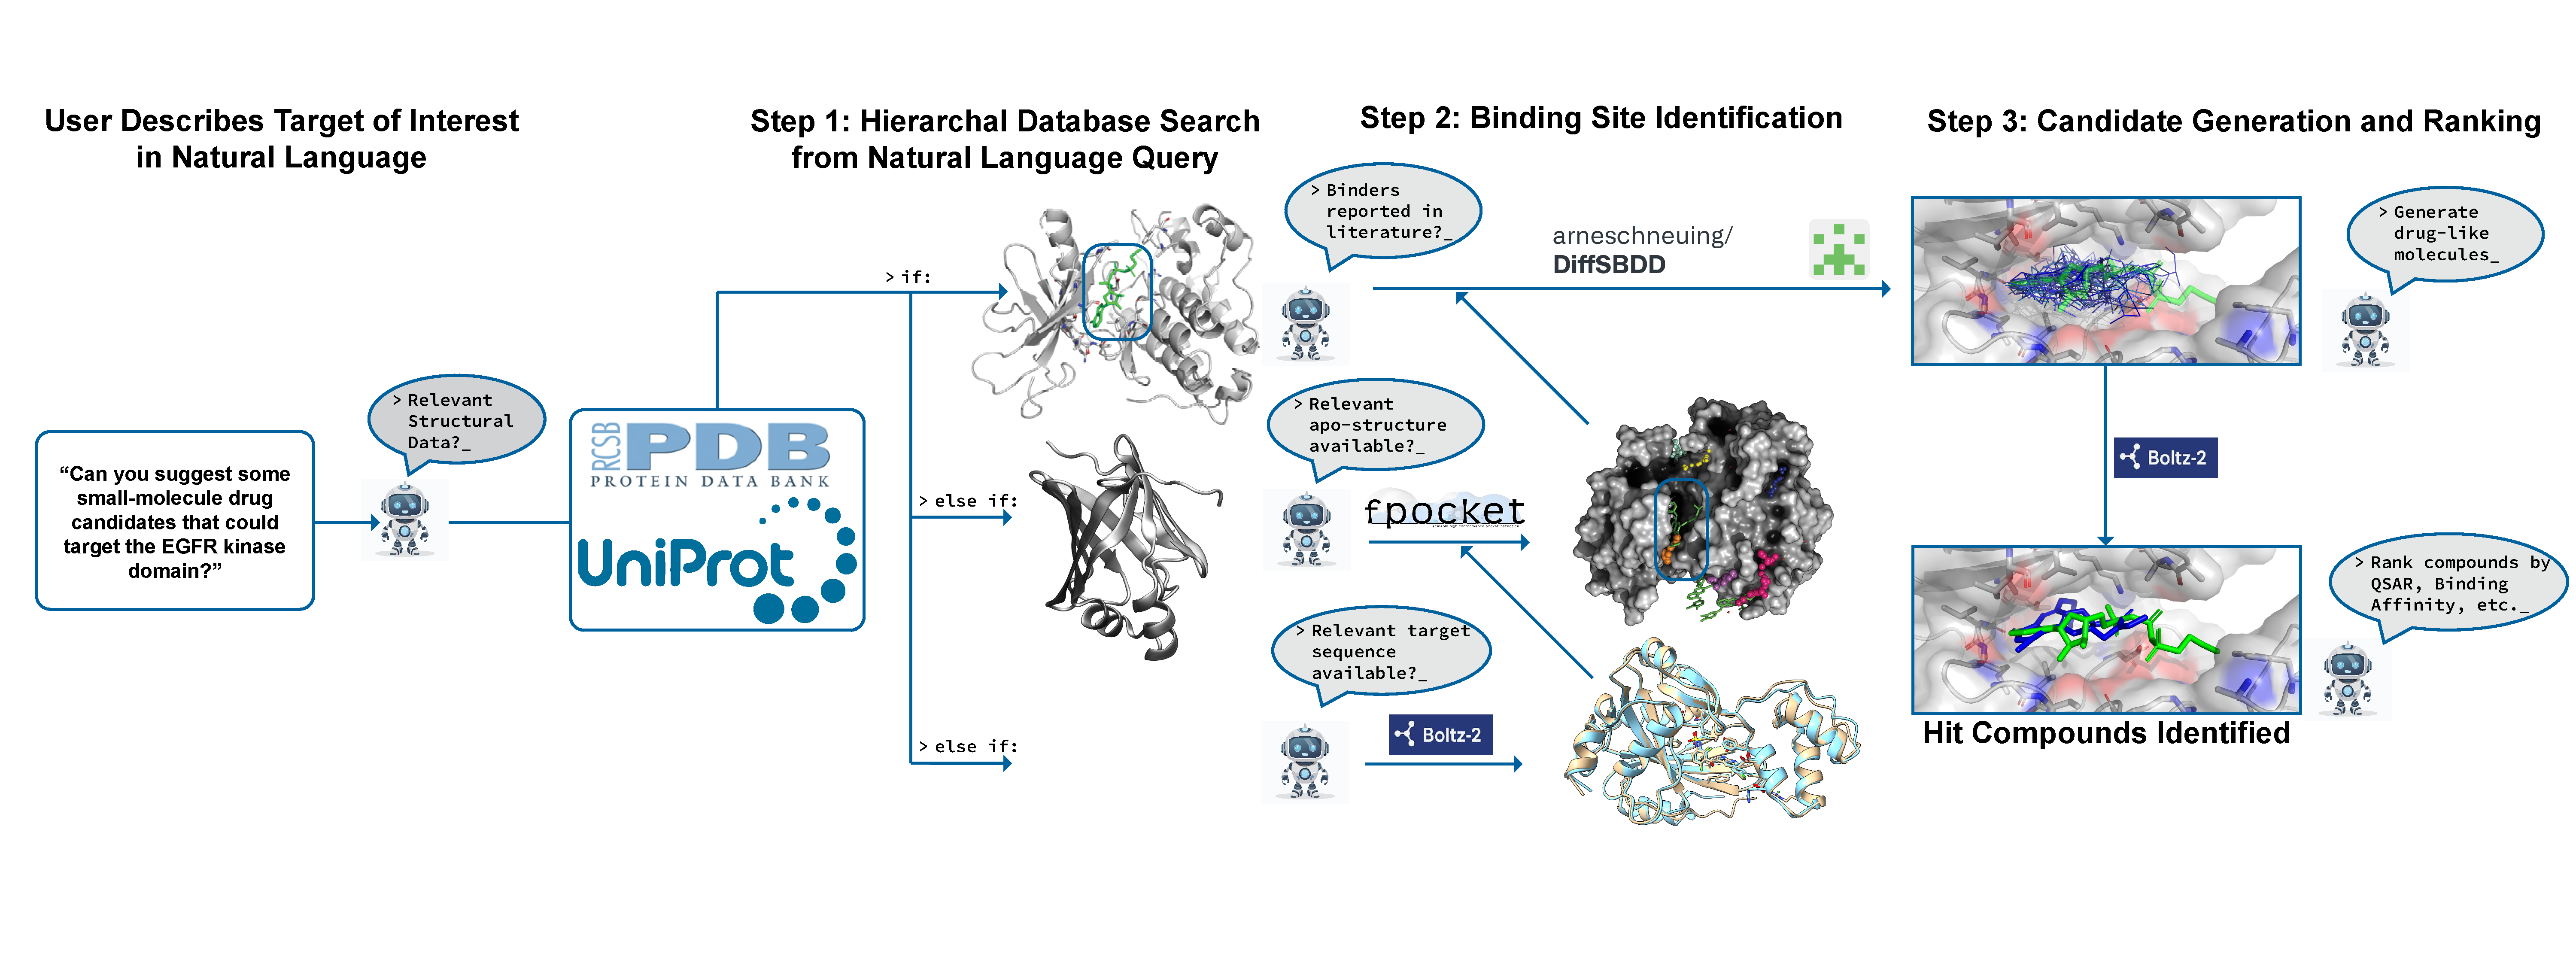
\includegraphics[width=1\linewidth]{figures/fade-workflow-overview.pdf}
    \caption{ \textbf{FADE workflow for natural language-driven drug candidate discovery.} The pipeline accepts user queries describing targets of interest (e.g., "Can you suggest some small-molecule drug candidates that could target the EGFR kinase domain?") and proceeds through three sequential steps: (1) hierarchical database search to identify relevant structural data, reported binders, apo-structures, or target sequences; (2) binding site identification; and (3) computational generation and ranking of drug-like molecules by QSAR and binding affinity metrics to identify hit compounds.}
    \label{fig:FADE-pipeline}
\end{figure}

\section*{Future Work}
Future work will focus on expanding the validation and applicability of the F.A.D.E platform. We plan to extend our analysis to a broader and more diverse set of benchmark systems, systematically evaluating F.A.D.E's performance across multiple target classes. This expanded validation will include rigorous comparison against established computational methods and, where available, experimental binding data. 

\section*{Open-source Materials}
Code is available on GitHub: \github{https://github.com/Naveen-R-M/F.A.D.E}

\section*{Author Contributions}
N.M.: Conceptualisation, Data Curation, Writing, Analysis, Visualisation, J.K: Software, Data Curation, Analysis, Visualisation, N.R.M.: Software, Data Curation, Analysis, X.Z.: Conceptualisation, Software, Data Curation, Analysis.
\end{teamsubmission}
% =====================================================================
%                 --- HACKATHON INFO ADDED HERE ---
% =====================================================================
\vspace{1.5em} % Add some vertical space before the main title
% =====================================================================

\begin{teamsubmission}{RealWorldChem}{MatFOMGen: A Collaborative Tool for Identifying Domain-Specific Chemical/Materials Figures-of-Merit for Autonomous Labs}
\authorsblock{
    Gopal R. Iyer\textsuperscript{1}\orcidlink{0000-0001-8117-6507}
}
\affiliationsblock{
    \textsuperscript{1}Lam Research Corporation (hackathon submission contributed independently)
}

\section*{Introduction}
MatFOMGen is a tool for autonomous/self-driving laboratories to rapidly identify appropriate computational targets, or figures-of-merit (FOMs), across diverse sub-domains of materials science and chemistry, toward which to direct their efforts in autonomous materials modeling, discovery, and synthesis. Self-driving labs have garnered significant academic \cite{ceder_alab, alabos} and private-sector interest in recent years due to their potential to accelerate the typically years-long research and development cycle that precedes the deployment of novel materials in industrial applications. A key differentiator in the ability of an autonomous laboratory to maintain a competitive position is its agility in pivoting to novel computational targets based on the highly variable nature of their potential industrial stakeholders. A self-driving lab may, for instance, be required to serve both the petrochemical industry and a client requiring novel high-entropy alloys using the same technological – software and hardware – stack. MatFOMGen is designed to address the materials-computational aspect of this challenge.

\section*{Results}
MatFOMGen begins with a user describing their domain of interest in natural language. An LLM-based agent then performs a web search of the relevant chemistry/materials science literature based on that domain and returns both a list of relevant computational targets (FOMs) that it identified and a comprehensive set of references that were consulted in the retrieval of each FOM. Each FOM is accompanied by a brief description and each paper is assigned a relevance score (0–1). The user then has the opportunity to select a subset of the FOMs for further analysis. Following the user's selection, MatFOMGen then generates, in stages, 1. detailed technical descriptions of the FOMs with the appropriate mathematical backgrouand, and 2. Atomic Simulation Environment (ASE) \cite{larsen2017atomic} functions that compute the FOMs requested by the user. In particular, ASE offers a placeholder for the \texttt{Calculator}, or level of theory (e.g. molecular dynamics), that is used to compute the FOM. This is because autonomous labs have often developed and offered custom machine learning interatomic potentials as key and proprietary offerings, which need to be evaluated in contexts relevant to their industrial stakeholders. The full workflow is summarized in Fig. \ref{fig:matfomgen_workflow}.

MatFOMGen utilizes LLMs in a modular, agentic, human-in-the-loop workflow. The initial literature review stage, the mathematical description stage, and the ASE function generation stage are all built to utilize different LLM calls. This affords the user flexibility in controlling the model capability and token usage that is allocated to each task. In our experience, smaller models offer satisfactory performance in fast literature review and FOM generation, while larger models offer greater accuracy in generating mathematical/technical descriptions and ASE functions.

\begin{figure}[h]
    \centering
\includegraphics[width=0.65\linewidth]{figures/MatFOMGen_Workflow_Schematic.png}
    \caption{MatFOMGen workflow.}
    \label{fig:matfomgen_workflow}
\end{figure}

MatFOMGen was built using the Anthropic API and Streamlit.

\section*{Future Work}
A key limitation of the current MatFOMGen pipeline is validation of the LLM-generated ASE functions. Future work may include additional LLM-based reflection/refinement steps. Another extension would be the use of fine-tuned LLMs for higher-accuracy function generation.

\section*{Open-source Materials}
The complete source code, documentation, and examples for MatFOMGen are openly available on GitHub at: \github{https://github.com/gopal-iyer/MatFOMGen}

\section*{Author Contributions}
G.R.I.: Conceptualization, software, writing, visualization.


\end{teamsubmission}



% %%%%%%%%%%%%%%%%%%%%%%%%%%%%%%%%%%%%%%%%%%%%%%%%%%%%%%%%%
% Team: DFTPilot  %
% %%%%%%%%%%%%%%%%%%%%%%%%%%%%%%%%%%%%%%%%%%%%%%%%%%%%%%%%%

\begin{teamsubmission}{DFTPilot}{DFTPilot: Automation and Previewing of DFT Calculation Setups}
\authorsblock{
    Savyasanchi Aggarwal\textsuperscript{1,4}\orcidlink{0009-0007-7128-3465},
    Chiku Parida\textsuperscript{2}\orcidlink{0009-0005-9938-5696},
    Diptendu Roy\textsuperscript{2}\orcidlink{0000-0001-7718-3018},
    Bingcan Li\textsuperscript{3}\orcidlink{0000-0002-1744-6397},
    Martin H. Petersen\textsuperscript{2}\orcidlink{0000-0001-5840-1796},
    Andre K.Y. Low\textsuperscript{4}\orcidlink{0000-0002-0985-5123}
}
\affiliationsblock{
    \textsuperscript{1} Department of Chemistry, University College London, London WC1E 6BT, United Kingdom\\
    \textsuperscript{2} Department of Energy Conversion \& Storage, Technical University of Denmark, Lyngby 2800, Denmark\\
    \textsuperscript{3} Department of Materials Science \& Metallurgy, University of Cambridge, Cambridge CB3 0FS, United Kingdom \\
    \textsuperscript{4} School of Materials Science \& Engineering, Nanyang Technological University, Singapore 639798, Singapore
}

\vspace{-3mm}
\section*{Introduction}

Computational and experimental materials research have both progressed quickly, but these communities are still somewhat separated. \textit{Density Functional Theory} (DFT) \cite{hohenberg1964inhomogeneous, kohn1965self} is a good example of this gap. Running DFT reliably often requires experience with convergence behaviour, functional choices, and numerical parameters \cite{squires2025guidelines}. This limits how widely DFT can be used outside of expert groups and slows the transfer of computational insight to experimental workflows.

Here we introduce \textbf{DFTPilot}, an intelligent assistant that aims to close this gap by using recent \textit{large language models} (LLMs) \cite{brown2020language,achiam2023gpt} to interpret DFT input and output files, connect new calculations to past work, and predict target properties. DFTPilot combines text-based reasoning with structured scientific data using \textit{retrieval-augmented generation} (RAG) \cite{lewis2020retrieval,izacard2020distilling} and graph-based regressors \cite{xie2018crystal,chen2019graph,himanen2020dscribe}. The system lets users query previous VASP calculations, inspect similar materials, and estimate properties such as bandgaps or total energies while taking the chosen functional into account \cite{perdew1996generalized,becke1988density}.

DFTPilot retrieves relevant OUTCAR files, predicts whether a calculation will converge under the current settings, and suggests updated INCAR parameters based on earlier runs. The overall idea is to help non-experts work effectively with DFT tools like VASP \cite{kresse1993ab, kresse1996efficient}, and to make first-principles modelling more accessible and easier to use in day-to-day research.

\vspace{-2mm}
\section*{Dataset}

Currently, DFTPilot is trained and indexed on a set of 426 DFT calculations collected from earlier ablation and convergence studies. These runs include standard relaxations performed with several exchange–correlation functionals (GGA, GGA+U, hybrid), and cover systems ranging from 4 to 120 atoms per cell. The dataset contains mostly metals and wide-bandgap oxides.

Each entry includes the initial structure, INCAR and POSCAR inputs, and the resulting OUTCAR file. To support both retrieval and prediction tasks, we built three embeddings:
(i) SentenceTransformers \cite{reimers2019sentencebert} embeddings for INCAR/OUTCAR text,
(ii) SOAP \cite{himanen2020dscribe} vectors for structural similarity, and
(iii) feature vectors for the CGCNN \cite{xie2018crystal} regressor.

We split the data by chemical and structural class, functional choice (GGA, GGA+U, HSE, PBE0), and calculation complexity (single-point, full relaxation, SOC-enabled), testing model generalisability. The dataset is still limited, especially for narrow-bandgap semiconductors and systems with different topologies, e.g. layered or amorphous materials, affecting the breadth of current predictions.
\vspace{-2mm}
\section*{Results}

DFTPilot connects LLMs with VASP \cite{kresse1993ab, kresse1996efficient} and associated pre-/post-processing tools to interpret and automate DFT workflows. The RAG system links new user queries to earlier DFT calculations, letting the model identify structurally or electronically similar materials. It also provides quick previews of OUTCAR files and estimates material properties directly from the input structure and INCAR parameters.

A crystal-graph neural network trained on the dataset reaches a mean absolute error of about 0.36 eV for bandgap prediction when restricted to materials with RAG similarity scores above 75\%. This is consistent with earlier CGCNN studies \cite{xie2018crystal}, and is notable given the limited dataset and incomplete use of INCAR information in the current prototype.

Across our splits, the framework generalises well on structurally distinct test cases and calculation types. Combined with multimodal embeddings, these results show that LLM-based systems can provide interpretable predictions and guidance on convergence behaviour directly from natural-language queries.

\begin{figure}[h]
\centering
\includegraphics[width=0.8\linewidth]{figures/dftpilot.png}
\caption{Schematic workflow for DFTPilot. The user specifies the target property and material system. The model returns \textbf{(a)} suggested INCAR updates and an OUTCAR preview, and \textbf{(b)} CGCNN-based property predictions using multimodal similarity metrics from the vector index.}
\label{fig:DFTPilot-pipeline}
\end{figure}
\vspace{-7mm}

\section*{Future Work}

Future extensions will expand the dataset with more materials classes, calculation types, and levels of theory. This added structural and chemical diversity will improve both the similarity index and performance of the property predictors. To improve coverage across the chemical space, we plan to add data from public sources such as NOMAD \cite{draxl2019nomad} and the Materials Project \cite{Jain2013}.

We also aim to extend the property prediction framework beyond bandgaps to include lattice parameters, dielectric tensors, and mechanical or electronic observables. These additions will help the system give more informative previews and support a more complete workflow from setup to property estimation.

\vspace{-2mm}
\section*{Open-source Materials}

Code, pre-trained weights, and the RAG index are available on GitHub:
\github{https://github.com/chiku-parida/DFTPilot}, and a demo video is here: \youtube{https://www.linkedin.com/feed/update/urn:li:activity:7372418332953763840/}

\vspace{-2mm}
\section*{Author Contributions}

\textbf{S.A}: Conceptualization, Software, Visualization, Writing (Original Draft);
\textbf{C.P}: Conceptualization, Software, Visualization, Writing (Editing);
\textbf{D.R}: Conceptualization, Software, Visualization, Writing (Editing);
\textbf{B.L}: Software;
\textbf{M.P}: Conceptualization, Writing (Editing);
\textbf{A.L}: Conceptualization
\end{teamsubmission}



% %%%%%%%%%%%%%%%%%%%%%%%%%%%%%%%%%%%%%%%%%%%%%%%%%%%%%%%%%
% Team: Parse Patrol  %
% %%%%%%%%%%%%%%%%%%%%%%%%%%%%%%%%%%%%%%%%%%%%%%%%%%%%%%%%%

\begin{teamsubmission}{Parse Patrol}{Parse Patrol: Dual-Mode Scientific Parsing Infrastructure via MCP Servers}
\authorsblock{
    Nathan Daelman\textsuperscript{1}\orcidlink{0000-0002-7647-1816},
    Christina Ertural\textsuperscript{2}\orcidlink{0000-0002-7696-5824},
    Rubel Mozumber\textsuperscript{1}\orcidlink{0009-0007-5926-6646},
    Sascha Klawohn\textsuperscript{1}\orcidlink{0000-0003-4850-776X},
    Remya Ann Mathews Kalapurakal\textsuperscript{3} 
}
\affiliationsblock{
    \textsuperscript{1}Humboldt University of Berlin, 10117 Berlin, Germany\\
    \textsuperscript{2}Department of Materials Chemistry, Federal Institute for Materials Research and Testing, 12205 Berlin, Germany\\
    \textsuperscript{3}University of New Hampshire, 03824 Durham, NH, USA
}

\section*{Introduction}

Parsing scientific files to extract structured data depends strongly on specifications.
These specifications may exist at a format level, a schema level, or more abstractly, an ontological one.
This dependency makes parser infrastructure very brittle and labor-intensive to maintain, as changes to either source or target specifications require updating parsers accordingly.
This is frequent in materials and chemistry databases and consortia. 

The rise of large language models (LLMs) has opened up new avenues for automating parser development, as modern models can reason over heterogeneous file formats and dynamically adapt to evolving specifications.
However, effective use of LLMs requires a reliable interface for connecting models to external tools.
Anthropic published the Model Context Protocol (MCP) in late 2024\cite{mcp2024}, providing a standardized interface for agents to discover and invoke external tools, access resources, and use predefined prompts\cite{mcp_def}.
It has since become the industry standard supported by all major commercial models.

In this work, we present Parse Patrol, an AI-assisted workflow for rapidly discovering, testing, and deploying parsers that conform to user-defined specifications.
Parse Patrol leverages MCP to integrate community parsers into a unified interface, enabling agents to iteratively evaluate parser options against target schemas.
The same infrastructure supports two usage modes:
(i) Discovery Mode, where an agent interactively tests parsers for schema conversion;
and (ii) Direct Import Mode, where the same parsers are available as Python modules for production code.

\section*{Results}

Automated parser generation faces several pitfalls:
scarce documentation for scientific specifications, model hallucinations outside training data, lengthy test iterations, and unstable software architectures.
Parse Patrol sidesteps these issues by leveraging community parsers, focusing instead on widening the source specification coverage and design options.
Because MCP provides a uniform, model-agnostic interface for invoking software tools, individual parsers can be exposed as MCP tools, allowing agents to orchestrate them seamlessly during parser selection, testing, and schema conversion.

MCP, however, does not prescribe how to organize tools: by default, servers simply expose a flat list of tools.
To address this, we define a \textit{hierarchical protocol} for structuring the MCP server.
Each parser is implemented as its own independent MCP server, which enables targeted feature development and testing.
These individual servers' components are then automatically registered with a central, user-facing server.
The central server aggregates all parser tools and resources, then adds prompts for test deployment and production workflows.
The user provides specifications either directly in the chat or as separate files, while test cases can be retrieved via database MCP servers.

While MCP tools enable interactive testing and one-off parsing tasks, bulk processing and production workflows require importable modules.
Parse Patrol addresses this by exposing the same parser both as an MCP server and as a Python module.
To ensure agents leverage these modules when writing code, we employ a two-pronged approach: prompts provide usage instructions, while each parser server exposes its module path and import syntax as an MCP resource.

Implementing this \textit{dual-mode design} (cf. Fig.\ref{fig:parse-patrol}) is challenging, as MCP servers and Python packages have different distribution requirements.
While the former are typically registered in the \href{https://github.com/modelcontextprotocol/servers}{MCP Registry}\cite{mcp2024registry}, the latter are distributed via \href{https://pypi.org/}{PyPi}\cite{pypi}.
Parse Patrol bridges this divide by maintaining a unified codebase that satisfies both frameworks' requirements, where each tool's schema serves both modes.
This ensures the tool interfaces evolve with use in both contexts.
To the best of the authors' knowledge, no other framework provides this dual-mode capability.

\begin{figure}[h]
    \centering
    \includegraphics[width=0.8\linewidth]{figures/parse-patrol.png}
    \captionsetup{width=\linewidth}
    \caption{
    Schematic depiction of the \textit{dual-mode} design in Parse Patrol.
    \textbf{Lower branch:} Discovery Mode provides a single MCP interface to several parser and database servers.
    An agent will use these to experiment with designing a parser conforming to the user-defined target specifications.
    \textbf{Upper branch:} Direct Import Mode exposes these same tools as Python modules for friction-less implementation based on the approaches learned during Discovery.
    \textbf{Both branches} are unified under a single architecture.
    }
    \label{fig:parse-patrol}
\end{figure}

\section*{Future Work}

At the time of writing, the repository is seeing active development.
Given the well-defined objective of providing a computational parsers toolkit, future extensions are not excluded.
This project is under consideration for incorporation into NOMAD parser suite\cite{nomad_lab,draxl2019nomad}.

\section*{Open Source Materials}

The open source code is available on GitHub: \github{https://github.com/ndaelman-hu/parse-patrol} (development version). For stable releases, consult the version tags. Submitted version for the hackathon: \texttt{v0.0.2-beta}.
A demo video is available on YouTube: \youtube{https://www.youtube.com/watch?v=fSAyi5ubkR0}.

\section*{Author Contributions}

\textbf{N.D.}: Conceptualization, Software, Original Code Draft, Visualization - Writing of Documentation and Manuscript, Editing
\textbf{C.E.}: Conceptualization Revision, Software, Visualization, Video Editing, Writing - Original Manuscript Text Draft, Figure, Editing
\textbf{R.M.}: Implementation asynchronous servers, Extension Testing Infrastructure - Conceptualization Revision, Proof-read Manuscript
\textbf{S.K.}: Extend Parser Servers - Proof-read Manuscript
\textbf{R.A.M.K.}: Testing of Setup, Trial new Parsers - Proof-read Manuscript

\section*{Acknowledgements}
This work was supported by the NFDI consortium FAIRmat - Deutsche Forschungsgemeinschaft (DFG) - Project 460197019.

\end{teamsubmission}



% %%%%%%%%%%%%%%%%%%%%%%%%%%%%%%%%%%%%%%%%%%%%%%%%%%%%%%%%%
% Team: Catalyst Assistant  %
% %%%%%%%%%%%%%%%%%%%%%%%%%%%%%%%%%%%%%%%%%%%%%%%%%%%%%%%%%

\begin{teamsubmission}{Catalyst Assistant}{Catalyst Assistant: Evidence-traced LLM Agent for $\mathrm{NH_3}$ Decomposition Catalysts}
\authorsblock{
    Wahid Billah\textsuperscript{1}\orcidlink{0009-0007-0214-0751},
    Md. Aqib Aman\textsuperscript{2}\orcidlink{0009-0007-3943-215X},
    M.A. Shadab Siddiqui\textsuperscript{3}\orcidlink{0009-0008-8525-3133},
    Abdullah Al Hasan\textsuperscript{4}\orcidlink{0009-0008-4820-9280},
    MD. Shaib Hossain\textsuperscript{5}\orcidlink{0009-0004-6663-5890},
    Shoaib Mahmud\textsuperscript{6}\orcidlink{0009-0002-3601-8467}
}
\affiliationsblock{
    \textsuperscript{1}Department of Architectural Engineering and Construction Management, King Fahd University of Petroleum and Minerals, Dhahran 31261, KSA.\\
    \textsuperscript{2}Department of Industrial and Systems Engineering, King Fahd University of Petroleum and Minerals, Dhahran 31261, KSA.\\
    \textsuperscript{3}Department of Materials Science and Engineering, King Fahd University of Petroleum and Minerals, Dhahran 31261, KSA.\\
    \textsuperscript{4}Department of Mechanical Engineering, King Fahd University of Petroleum and Minerals, Dhahran 31261, KSA.\\
    \textsuperscript{5}Department of Mechanical Engineering, Chittagong University of Engineering \& Technology, Bangladesh.\\
    \textsuperscript{6}Department of Computer Science and Engineering (CSE), BRAC University, Bangladesh.\\
}

\section*{Introduction}
Catalyst Assistant, an evidence-bound AI co-researcher built to accelerate ammonia (\ce{NH3}) decomposition catalyst discovery. It proposes and ranks candidates, plans synthesis/testing, and auto-generates XRD/BET visuals by fusing curated literature, datasets, and APIs (e.g., Materials Project) through context-engineered modules that minimize hallucinations. ChatGPT is customized to reduce hallucinations, with methods designed to support academics, industry practitioners, and students. The outcome is faster, safer screening with structured, reproducible outputs for researchers and learners alike.

\section*{Results}
This architecture demonstrates how GPT-5 operates with the Catalyst Assistant to address user inquiries through a systematic workflow. The frontend facilitates user engagement, where individuals submit queries and data while receiving structured outputs such as tables, reports, visualizations, and explanations. The backend integrates three fundamental modules working in coordination: the Knowledge module supplies diverse information sources including datasets, PDFs, and APIs; the Context Engineering module applies structured prompting techniques, routing rules, verification guardrails, and data source integration pathways; and the Reasoning module validates contextual accuracy and data integrity. Through Agentic Routing, GPT-5 connects these backend components seamlessly, utilizing chat history to maintain contextual continuity throughout interactions. This architectural framework represents a comprehensive system that combines knowledge retrieval, intelligent coordination, and validation mechanisms to generate accurate, contextually relevant responses aligned with user requirements and specific task objectives. 

\begin{figure}[H]
    \centering
    \includegraphics[width=0.7\linewidth, height=0.4\textheight, keepaspectratio]{figures/System Architecture - Catalyst Assistant.png}
    \caption{System Architecture of Catalyst Assistant}
    \label{fig:System Architecture - Catalyst Assistant}
\end{figure}

\section*{Future Work}

Next, the pipeline will be hardened with a dedicated data-extraction/plotting service and hosting API to improve figure accuracy and reproducibility, addressing current limitations. Uncertainty-aware ranking and automated synthesis/test planners will also be added so that they can tap more materials databases  for broader, non-precious catalyst discovery and experiment-ready outputs.

\section*{Open-source Materials}
The LLM agent is available here: \url{https://chatgpt.com/g/g-68c09896f11c81918e86b7ddcbad47e3-catalyst-assistant}.
A demo video is available on YouTube: \youtube{https://youtu.be/4uqrp6kbK4s}.


\section*{Author Contributions}
\textbf{W.B.}: Conceptualization; Methodology; Formal analysis; Visualization; Writing – Original Draft. \textbf{M.A.A.}: Conceptualization; Methodology; Formal analysis; Visualization; Writing – Original Draft. \textbf{M.A.S.S.}: Conceptualization; Methodology; Formal analysis; Visualization; Writing – Original Draft; Validation. \textbf{A.A.H.}: Resources; Validation. \textbf{M.S.H., S.M.}: Data collection; Data curation.


% References to MCP, Gaussian etc. 

\end{teamsubmission}



% %%%%%%%%%%%%%%%%%%%%%%%%%%%%%%%%%%%%%%%%%%%%%%%%%%%%%%%%%
% Team: ThinFilm.ai  %
% %%%%%%%%%%%%%%%%%%%%%%%%%%%%%%%%%%%%%%%%%%%%%%%%%%%%%%%%%

\begin{teamsubmission}{ThinFilm.ai}{Data-Driven Prediction of Thin Film Properties in Physical and Chemical Deposition Methods}
\authorsblock{
    Ram Munde\textsuperscript{1}\orcidlink{0009-0001-5597-1213},
    Lena Ara\textsuperscript{2}\orcidlink{0009-0007-0198-0871}
}
\affiliationsblock{
    \textsuperscript{1}Department of Materials Engineering, Purdue University, West Lafayette, USA\\
    \textsuperscript{2}Elmore Family School of Electrical and Computer Engineering, Purdue University Indianapolis, USA\\
}

\section*{Introduction}


ThinFilm.ai is a multimodal AI framework for predicting thin film quality, designed to fuse structured deposition data with unstructured text from a corpus of 100 research papers. We specially focused on studies that included characterization data such as x-ray photoelectron spectroscopy (XPS), scanning electron microscopy (SEM), and  x-ray diffraction (XRD). A supervised pipeline utilizes three classification models, trained on data extracted via the GPT-4 API, to predict key quality metrics: crystallinity, impurity, and roughness. Concurrently, an unsupervised pipeline generates domain-specific MatSciBERT embeddings from the "Results" sections of the literature. These text embeddings are concatenated with structured feature vectors and clustered to discover latent relationships, with KeyBERT subsequently employed for thematic keyphrase extraction, leveraging BERT-based similarity, to provide interpretable labels for each cluster related to film quality and fabrication parameters.
The final Streamlit-hosted platform synthesizes these quantitative predictions and qualitative insights, delivering a unified analysis for materials researchers.

\section*{Results}
Figure \ref{fig:thinfilm} demonstrates the workflow. This project aims to address a critical challenge in experimental materials science: predicting thin film quality from deposition recipes before exhaustive lab experiments are performed. The final results are synthesized in our Streamlit app, which provides instant predictions of crystallinity, roughness, impurity composition, and interface quality.
\begin{figure}[H]
    \centering
    \includegraphics[width=\linewidth, height=0.4\textheight, keepaspectratio]{figures/thinfilm.jpg}
    \caption{Data extraction methods and model process flow}
    \label{fig:thinfilm}
\end{figure}

\section*{Future Work}
Future work includes data augmentation by ingesting more comprehensive datasets, refining preprocessing pipelines and expanding the feature set to include key deposition parameters such as pressure, temperature, and deposition time for more accurate insights. Concurrently, we will explore architectural optimizations, such as knowledge graphs, to better represent complex deposition techniques data. Finally, we will pursue model enhancement through rigorous fine-tuning and training of more robust models to increase predictive accuracy.



\section*{Open-source Materials}

Code and pretrained weights available on GitHub: \url{https://github.com/ram123-debug/mat-chem-llm-hackathon.git}\\
A demo video is available on YouTube: \url{https://youtu.be/dazb9VQNvOY}.

\section*{Author Contributions}

\textbf{Lena Ara:} Conceptualization, Writing, review \& editing, Methodology, Investigation, Formal analysis.\\ \textbf{Ram Munde:} Conceptualization, Writing, review \& editing, Methodology, Investigation, Formal analysis. 

\end{teamsubmission}



% %%%%%%%%%%%%%%%%%%%%%%%%%%%%%%%%%%%%%%%%%%%%%%%%%%%%%%%%%
% Team: SCALE  %
% %%%%%%%%%%%%%%%%%%%%%%%%%%%%%%%%%%%%%%%%%%%%%%%%%%%%%%%%%

\begin{teamsubmission}{SCALE}{Scaffold Conscious Agent for Learning \& Exploration}
\authorsblock{
    Sruthy K Chandy\textsuperscript{1}\orcidlink{0000-0002-1061-647X},
    Vivek Pandit\textsuperscript{2}\orcidlink{0009-0000-9121-6066},
    Ashwini Verma\textsuperscript{3}\orcidlink{0000-0001-9837-9597}
}
\affiliationsblock{
    \textsuperscript{1}University of California, Berkeley, CA, USA\\
    \textsuperscript{2}Chipstack, San Jose, CA\\
    \textsuperscript{3}CSIR-National Chemical Laboratory, Dr Homi Bhabha Road, Pune, India
}

\section*{Introduction}
The design and optimization of functional small molecules underpin advances in drug discovery, materials development, and chemosensory science. Despite major progress in deep generative modeling, most existing approaches still struggle to maintain chemical validity, preserve pharmacophoric scaffolds, or produce synthetically feasible compounds \cite{sanchez2018inverse}. At the same time, large language models (LLMs) have demonstrated powerful reasoning and symbolic manipulation capabilities, enabling new opportunities for chemistry-aware design frameworks \cite{elton2019deep}. However, their direct application to molecular generation is limited by hallucinations, lack of physical grounding, and the absence of adaptive feedback loops.

To address these challenges, we developed SCALE (Scaffold-Conscious Agent for Learning and Exploration), an LLM-driven molecular optimization framework that couples reasoning-based molecular edits with cheminformatics guardrails and lightweight physics-aware scoring. SCALE allows scaffold-preserving exploration of chemical space for diverse applications, including drug discovery, fragrance design, and repellent or agrochemical screening, all within an interpretable and iterative optimization loop.
\section*{Results}
The SCALE framework operates as an adaptive, closed-loop optimization system that unites the reasoning capacity of large language models (LLMs) with the quantitative rigor of cheminformatics and physics-based scoring. The process begins with one or more seed molecules that define the structural scaffolds and property targets of interest. These seeds constrain the search space, ensuring that subsequent modifications retain core pharmacophores or functional groups relevant to biological or sensory function. SCALE can therefore operate flexibly across application domains such as drug discovery, fragrance and flavor chemistry, or repellent and agrochemical design.

An LLM controller acts as the generative engine, proposing scaffold-preserving edits such as R-group substitutions, heteroatom replacements, or ring decorations. Unlike statistical generative models, the LLM uses explicit textual reasoning, incorporating feedback from previous rounds to refine its chemical intuition. Each generated molecule undergoes a multi-layered guardrail evaluation that verifies SMILES validity, eliminates PAINS and reactive motifs, and estimates synthetic accessibility. Molecules that meet these cheminformatics criteria are then analyzed with lightweight physical descriptors like MMFF94 strain energy, QED, SA score, and logP to assess structural stability and drug-likeness. These filters collectively prevent the propagation of chemically implausible or synthetically inaccessible candidates.

To enable rapid and uncertainty-aware property estimation, SCALE employs a Random Forest (RF) surrogate model trained on molecular descriptors and precomputed physicochemical features. The surrogate predicts mean property values ($\mu$) and associated uncertainties ($\sigma$), which are combined through the Upper Confidence Bound (UCB = $\mu$ + $\kappa$$\sigma$) criterion to balance exploitation of promising molecules and exploration of uncertain regions of chemical space\cite{he2023structured}. Candidates exceeding a dynamic UCB threshold are retained, while the rest are discarded or used to update the model’s exploration bias. Feedback from this layer guides the LLM’s next sequence of scaffold edits, forming a self-correcting optimization loop that continues until convergence criteria plateaued property improvement, diversity saturation, or iteration limits—are reached. Through this integration of LLM reasoning, chemical guardrails, and physics-informed uncertainty modeling, SCALE establishes an interpretable and efficient pathway for hit identification and lead optimization in both pharmaceutical and chemosensory molecular design.

\begin{figure}[H]
    \centering
    \includegraphics[width=\linewidth, height=0.4\textheight, keepaspectratio]{figures/scale_diagram_workflow.png}
    \caption{SCALE Workflow diagram}
    \label{fig:scale}
\end{figure}

\section*{Future Work}
Future extensions of SCALE will focus on enhancing both its chemical accuracy and autonomy by integrating higher fidelity physics and adaptive learning. Incorporating semiempirical or DFT-level calculations (e.g., GFN2-xTB, $\omega$B97X-D) into the surrogate model would improve the reliability of property predictions beyond empirical descriptors, while active learning loops could retrain the Random Forest dynamically as the chemical space expands. Replacing the RF surrogate with a graph neural network or a multi-task ensemble would allow simultaneous optimization of multiple properties, including target affinity, toxicity, and volatility. Fine-tuning the LLM controller on chemically curated corpora or reaction based transformations could reduce hallucinations and improve context aware molecular reasoning. Additionally, coupling SCALE with automated synthesis planning and experimental validation pipelines could transform it into a fully closed-loop discovery platform. Finally, benchmarking SCALE against established generative frameworks such as REINVENT, MolDQN, or GFlowNet would quantitatively establish its efficiency and generalizability across chemical domains.

\section*{Open Source Materials}
Code available in github repo: \github{https://github.com/schandy2211/scale}\\
A demo video is available on Youtube: \youtube{https://youtu.be/k0Y7rfM3rLY?si=TOZxu3DYb_vBUStO}

\section*{Author Contributions}
\textbf{S.K.C.}: Conceptualization, Data Curation, Investigation, Formal Analysis, Methodology, Software, Writing – original draft. 
\textbf{V.P.}: Conceptualization, Software, Project administration, Formal Analysis, Investigation, Writing – original draft. 
\textbf{A.V.}: Conceptualization, Methodology, Resources

\end{teamsubmission}



% %%%%%%%%%%%%%%%%%%%%%%%%%%%%%%%%%%%%%%%%%%%%%%%%%%%%%%%%%
% Team: L.A.R.A  %
% %%%%%%%%%%%%%%%%%%%%%%%%%%%%%%%%%%%%%%%%%%%%%%%%%%%%%%%%%

\begin{teamsubmission}{L.A.R.A}{LLM as Aerogel Research Assistant}
\authorsblock{
    Sugan Kanagasenthinathan\textsuperscript{1}\orcidlink{0009-0004-6821-0378},
    Prakul Pandit\textsuperscript{1}\orcidlink{0000-0002-1343-3046},
    Hemangi Patel\textsuperscript{1}
    }
\affiliationsblock{
    \textsuperscript{1} Institute for Frontier Materials on Earth and in Space, German Aerospace Center, Cologne, Germany\\
}
\section*{Introduction}

Aerogels are highly open-porous nanostructured materials, that are among the most versatile porous materials. They exhibit exceptional material properties porous nanostructured morphology. They typically possess very
low densities, high porosity, and
low thermal conductivities \cite{aegerter2011aerogels}, yet their development remains slow due to complex multi-scale synthesis pathways and fragmented knowledge across literature. Recent advances in large language models have opened new possibilities for automated scientific reasoning. Our framework L.A.R.A addresses this opportunity by combining a fine-tuned LLaMat \cite{mishra2025foundationallargelanguagemodels} model with a materials knowledge graph and a modular tool ecosystem, enabling structured hypothesis generation, synthesis planning, and characterization workflows. The framework is designed as a research assistant tailored specifically to aerogel science while remaining extendable for other similar porous material classes, e.g hydrogels and xerogels.
\section*{Results}

L.A.R.A consists of three core components: (1) a fine-tuned language model specialized for aerogel synthesis and characterization, (2) a knowledge-graph interface built on MatKG \cite{venugopal2024matkg} for structured reasoning, and (3) a tool ecosystem supporting literature search, molecular simulations, and image-based characterization.  

The model is fine-tuned on more than one thousand expert-curated aerogel synthesis examples using LoRA parameter-efficient training with a maximum sequence length of 1024 tokens and a learning rate of \( 10^{-5}\). Knowledge-graph integration maps scientific questions to materials entities, properties, and synthesis relationships, enabling grounded hypothesis generation. The tool ecosystem includes microscopy-image segmentation, RAG-based literature search, and MD simulation modules orchestrated through a multi-agent interface.\par

\begin{figure}[h!]
    \centering
    \includegraphics[width=0.85\textwidth]{figures/Fine tuned Llamat Model.jpg}  % replace with your file name
    \caption{Architecture and workflow of L.A.R.A. The fine-tuned model determines whether to respond using the knowledge ingestion layer, leveraging either direct fine-tuning or the knowledge graph, or to utilize one of the tools available in the interface layer.}

    \label{fig:lara}
\end{figure}
The fine-tuned model demonstrates strong performance in both scientific reasoning and synthesis-route generation for  aerogels. Benchmarked against expert-annotated queries, L.A.R.A produced relevant hypotheses and generated plausible synthesis routes consistent with known sol-gel chemistry. The framework also supports inverse design queries where target properties are specified directly; for example, requesting porosity above 0.95 combined with a minimum electrical conductivity returns multiple synthesis pathways supported by mechanistic scientific rationales. A complete research workflow is shown in Figure~\ref{fig:lara}.

In addition to these domain-specific capabilities, L.A.R.A incorporates an agentic decision layer that enables the model to determine, for each user query, whether direct reasoning is sufficient or whether external tool invocation is required. This decision process is governed by both the semantic content of the user prompt and the structured descriptions of the available tools. When a query is self-contained, for instance, a conceptual question regarding sol-gel reaction mechanisms, the LLM performs internal reasoning and responds without invoking external computation. Conversely, when the semantic structure of the prompt corresponds to an operation that requires empirical grounding or numerical evaluation (e.g., ``search recent papers on RF aerogels'', ``analyze this SEM image'', or ``run a molecular dynamics simulation for silica clustering''), the model infers that the task exceeds its internal capabilities and selects the appropriate external tool.

This inference arises from a representation-alignment process in which the user’s request and each tool’s functional description are projected into a shared latent space, allowing the model to assess their compatibility. If the required evidence, cannot be produced through internal reasoning alone, the system routes the query to the tool whose operational description most closely matches the inferred objective. Table~\ref{tab:model_comparison} summarizes the key differences in inference and reasoning capabilities between L.A.R.A and ChatGPT (GPT 5.1) for the tasks of hypothesis generation and inverse design of aerogels.

\begin{table}[h!]
\centering
\caption{ Comparison of ChatGPT (GPT-5.1) and L.A.R.A Responses}
\label{tab:model_comparison}
\small
\begin{tabular}{|p{3.5cm}|p{5cm}|p{5cm}|}
\hline
\textbf{Evaluation Criteria} & \textbf{ChatGPT (GPT-5.1)} & \textbf{L.A.R.A} \\
\hline
Response Philosophy & Educational and conceptual framework focused on understanding principles & Hypothesis-driven scientific analysis with research-oriented insights \\
\hline
Output Structure & Sequential stage-based frameworks (3-4 stages) with clear progression & Multiple ranked hypotheses (5 hypotheses) with confidence intervals  \\
\hline
Technical Specificity & Identifies materials and methods conceptually without specific values & Provides specific parameters: temperature ranges, time frames, chemical formulas \\
\hline
Ethics \& Safety & Explicitly refuses to provide actionable lab procedures, temperatures, concentrations, or step-by-step instructions & Mentions safety concerns and processing challenges as part of technical discussion \\
\hline
Quantitative Information & Avoids providing specific numerical parameters (temperatures, ratios, times) & Includes specific numerical values (400-1200°C, several hundred bars, and confidence intervals between 0 to 1) \\
\hline
Scientific Depth & Explains underlying chemistry, mechanisms, and property relationships conceptually & Discusses molecular mechanisms (sp$^2$ hybridization), interfacial interactions, and structural characteristics \\
\hline
Practical Applicability & Non-actionable content designed for education and understanding, not direct implementation & Partially actionable with technical depth suitable for researchers familiar with laboratory protocols \\
\hline
\end{tabular}
\end{table}


\section*{Future Work}

Upcoming extensions include expanding the fine-tuning dataset to additional aerogel families. While the current system employs a tool setup, an ideal way ahead would be to implement the interaction via a Model Context Protocol (MCP) layer. Moreover, the finetuned LLM is enhanced with a MatKG which lacks comprehensive information and entity relationships for the aerogels. Thus further work needs to improve the data by extending the MatKG graph for aerogel use-cases. Furthermore, from an agentic perspective, the current system executes only single-step tool calls in which the LLM invokes one tool, receives its output, and immediately returns a response to the user; there is no capability for iterative tool reasoning, chaining multiple tools, or orchestrating multi-step plans to reach a target outcome. Future versions will therefore incorporate multi-tool, multi-turn agentic workflows to enable autonomous decision-making and sequential tool utilisation.

\section{Open-Source Materials}

The open-source implementation of L.A.R.A Module~2, including model-fine-tuning scripts, tools, and demonstration, is available at:  
\github{https://github.com/sugannathan/L.A.R.A-LLMs-as-Aerogel-Research-Assistants/tree/main}


\section*{Author Contributions}

\textbf{SK}: Data Curation, Software and Architecture, Model finetuning,  Writing;
\textbf{PP}: Conceptualization, Software and architecture, Writing, Project Administration;
\textbf{HP}: Software, Visualisation and Presentation

\end{teamsubmission}



% %%%%%%%%%%%%%%%%%%%%%%%%%%%%%%%%%%%%%%%%%%%%%%%%%%%%%%%%%
% Team: ODE FORGE %
% %%%%%%%%%%%%%%%%%%%%%%%%%%%%%%%%%%%%%%%%%%%%%%%%%%%%%%%%%

\begin{teamsubmission}{ODE FORGE}{Agentic AI for Autonomous Research and Simulation of Differential Equation Models}
\authorsblock{
    Souvik Ta\textsuperscript{1}\orcidlink{0009-0009-5747-7639}
}
\affiliationsblock{
    \textsuperscript{1} Dept. of Chemical and Biochemical Engineering, Western University, Ontario, Canada\\
}
\section*{Introduction}
Modeling dynamic systems with Ordinary Differential Equations (ODEs) is a cornerstone of research in materials science and chemistry. However, the process of translating theoretical models from literature into rigorous, runnable computational simulations is often a manual bottleneck, requiring significant programming expertise that can separate domain experts from rapid experimentation. ODE Forge addresses this challenge by automating the research-to-analysis workflow. By leveraging a multi-agent Large Language Model (LLM) framework, it bridges the gap between natural language scientific queries and immediately runnable, interactive simulations, empowering researchers to focus on scientific inquiry rather than on implementation details.

\section*{Methodology}
ODE Forge employs a two-phase agentic workflow (Figure~\ref{fig:odeforge_architecture}) composed of conversational research and autonomous coding/execution. Each phase is implemented as a LangGraph \cite{langchain2023} graph, with nodes representing specialized agents.

\subsection*{Phase 1 – Conversational Research}
The user begins by initiating an interactive dialog describing the target system, such as a request to simulate the Lotka–Volterra equations with specific rate constants. The large language model (LLM) agent queries both an embedded paper library, which can be uploaded by the user, and external web sources to construct a comprehensive model specification. This specification includes the differential equations governing the system, relevant parameters and initial conditions, solver preferences such as Runge--Kutta or stiff solvers, and the required forms of analysis or visualization. When relevant literature is available, the retrieval-augmented generation (RAG) mechanism~\cite{lewis2020retrieval} prioritizes the trusted local corpus to maintain domain-specific fidelity. The resulting structured specification is serialized as a JSON file and passed seamlessly to the autonomous coding phase.
\subsection*{Phase 2 – Autonomous Coding and Execution}
In the second phase (Figure~\ref{fig:odeforge_architecture}), an automated coding agent transforms the specification into a complete and executable Python script. The agent initializes the project environment, defines all equations and parameters, and integrates the solver and plotting routines before executing the script within a Docker sandbox to ensure safety and reproducibility. During execution, a self-healing debug loop continuously monitors the sandbox output. When an error occurs, the agent interprets the traceback, edits the code, and re-runs the script autonomously until its successful completion. The final artifacts-- \texttt{script.py}, \texttt{plot.png}, and \texttt{data.csv} --are generated automatically and exported to the results dashboard for user inspection and post-processing.

\section*{Technical Implementation}

ODE Forge is implemented in Python using LangGraph to orchestrate a multi-agent workflow over a structured state. This state tracks the full conversation, the evolving problem specification (model description, symbolic equations, parameters, initial conditions, and simulation settings), as well as the generated solver code, execution status, and debugging information. Maintaining a unified state allows the system to transition cleanly from interactive research to fully automated code generation and simulation.

In the conversational phase, a LLM agent incrementally builds the specification by asking targeted questions and, when needed, invoking specialized tools. These include a web researcher (via Tavily search), a local RAG expert who queries a Chroma vector store built from user-uploaded PDFs~\cite{lewis2021retrievalaugmentedgenerationknowledgeintensivenlp}, and a specification tool that writes confirmed content back into the specification fields. The local library is persisted on disk so that it can be reused across sessions without rebuilding the index on every run.

Once the user confirms that the specification is complete control passes to the coding phase. The system constructs a Python script in stages: it starts from a template, asks the LLM to translate the symbolic equations into SymPy code and the textual parameters and initial conditions into executable assignments, and then generates SciPy calls together with plotting and CSV export logic \cite{DBLP:journals/corr/abs-1907-10121}. The completed script is executed inside an isolated Docker image to ensure safety and reproducibility. If execution fails, the captured traceback is fed back to the model, which proposes a revised script; this closed-loop repair cycle repeats up to a fixed retry limit.

\captionsetup{type=figure,width=\textwidth}
\begin{figure*}[t]
    \centering
    \begin{minipage}{0.49\textwidth}
        \centering
        \includegraphics[width=\linewidth]{figures/Image1ODEForge.png}
    \end{minipage}
    \hfill
    \begin{minipage}{0.49\textwidth}
        \centering
        \includegraphics[width=\linewidth]{figures/Image2ODEForge.png}
    \end{minipage}
\caption{Workflow of ODE Forge showing (left) the two-phase agentic pipeline for research and model construction, and (right) the internal automated coder process for script generation, debugging, and execution within a Docker sandbox.}
\label{fig:odeforge_architecture}
\end{figure*}
\section*{Open-source Materials}
The code for ODEForge is available on Github at this repository: \github{https://github.com/souvikta/ODEForge}
\section*{Discussion}
The ODE Forge framework demonstrates how agentic AI can operate as an active scientific collaborator \cite{Decardi_Nelson_2024,Boiko2023} rather than a passive assistant. Beyond understanding natural language prompts, it performs structured reasoning that couples symbolic mathematics, literature retrieval, and iterative verification. This architecture embodies a reproducible paradigm for future AI laboratories in which conversational specification replaces manual scripting, autonomous debugging guarantees self-reliance, and sandbox execution preserves scientific rigor.

Although current implementations focus on ordinary differential equation systems, the same principles can be extended to partial differential equations, stochastic simulations, and optimization problems by introducing domain-specific solver modules and tool adapters. The system’s limitations arise primarily from dependence on LLM reasoning for equation parsing and a lack of current support for multi-physics coupling.

\end{teamsubmission}



% %%%%%%%%%%%%%%%%%%%%%%%%%%%%%%%%%%%%%%%%%%%%%%%%%%%%%%%%%
% Team: MP-LLM %
% %%%%%%%%%%%%%%%%%%%%%%%%%%%%%%%%%%%%%%%%%%%%%%%%%%%%%%%%%

\begin{teamsubmission}{MP-LLM}{MP-LLM: Materials Project Query Interface}
\authorsblock{
    Juno Nam\textsuperscript{1,*}\orcidlink{0000-0002-9506-2938},
    Killian Sheriff\textsuperscript{1,*}\orcidlink{0000-0003-3613-2948},
    Akshay Subramanian\textsuperscript{1,*}\orcidlink{0000-0002-9184-9979}
}
\affiliationsblock{
    \textsuperscript{1}Department of Materials Science and Engineering, Massachusetts Institute of Technology\\
    \textsuperscript{*}All authors contributed equally to this work, the order is alphabetical.\\
    % \textsuperscript{3}Affiliation 3
}

% --- Summary Guideline instructions replaced with prose below ---

\section*{Introduction}
Accessing large scientific databases, such as the Materials Project (MP) \cite{Jain2013}, typically requires a detailed understanding of the MP API client syntax as well as knowledge of the available API endpoints, creating a barrier to entry. To address this, we introduce MP-LLM, an interface that translates natural language queries into structured API calls. This tool democratizes access to materials data by enabling researchers to query the MP database using conversational language.

\begin{figure}[H]
    \centering
    \includegraphics[width=\linewidth, height=0.3\textheight, keepaspectratio]{figures/ui.png}
    \caption{User interface to perform Materials Project queries.}
    \label{fig:mp-llm-ui}
\end{figure}

\section*{Results}
Our system provides a simple web interface (Figure~\ref{fig:mp-llm-ui}) where users input natural language prompts, such as ``find all stable oxides with a band gap over 2 eV.'' This query is processed by a user-selected model, which generates a structured YAML query for the official Materials Project API. We evaluated two distinct methods: \textit{direct} generation, where the model attempts to output material IDs, and \textit{tool-augmented} generation, where the model generates the formal API query. Our benchmarks (Figure~\ref{fig:mp-llm-benchmark}) show that tool augmentation is critical for this task. The \textbf{Gemini 2.0 Flash [tool]}~\cite{Gemini} method achieved the highest performance, with a balanced F1 score of 72.3\% (74.3\% precision, 71.4\% recall). In contrast, \textit{direct} generation methods like \textbf{GPT-5 [direct]}~\cite{openai2024gpt4technicalreport} failed, scoring 0\% recall and 2.5\% precision, proving this approach is unsuitable. The tool-augmented method provides a more robust and effective strategy for natural language queries.

\begin{figure}[H]
    \centering
    \includegraphics[width=\linewidth, height=0.3\textheight, keepaspectratio]{figures/benchmark_result.png}
    \caption{Benchmark results for various model choices. Tool-augmented methods are generally more performant than direct generation methods across tested queries.}
    \label{fig:mp-llm-benchmark}
\end{figure}

\section*{Future Work}
Future work will include natural language visualization that converts prompts into chart specifications linked to MP API results, suggesting appropriate defaults, enabling interactions, and supporting export of figures and reproducible code. We will also add built-in post-processing triggered by short text instructions, such as filtering by stability thresholds, normalizing formulas, aggregating by crystal system, computing simple derived properties, and flagging outliers, with input validation and provenance tracking.

\section*{Open-source Materials}
The code for MP-LLM is available on GitHub: \github{https://github.com/killiansheriff/MP-LLM}. 

\section*{Author Contributions}
 \textbf{Juno Nam:} Conceptualization, Software, Writing. 
 \textbf{Killian Sheriff:} Conceptualization, Software, Writing.
 \textbf{Akshay Subramanian:} Conceptualization, Software, Writing.
 All authors contributed equally to this work, the order is alphabetical.
 
\end{teamsubmission}



% %%%%%%%%%%%%%%%%%%%%%%%%%%%%%%%%%%%%%%%%%%%%%%%%%%%%%%%%%
% ATOMS Lab %
% %%%%%%%%%%%%%%%%%%%%%%%%%%%%%%%%%%%%%%%%%%%%%%%%%%%%%%%%%

\begin{teamsubmission}{ATOMS Lab}{PALS: Property Analogies with LLMs}
\authorsblock{
    Alexander J. Haibel\textsuperscript{1,2}\orcidlink{0009-0001-6249-5219},
    Fariha Agbere\textsuperscript{1}\orcidlink{0009-0004-9090-8166},
    Samiha Sharlin\textsuperscript{1}\orcidlink{0000-0002-6379-9206},
    Faezeh Shahmoradi\textsuperscript{1},\\
    Kevin Ishimwe\textsuperscript{2}\orcidlink{0009-0008-4551-4570},
    Tyler R. Josephson\textsuperscript{1,2}\orcidlink{0000-0002-0100-0227}
}
\affiliationsblock{
    \textsuperscript{1} \small{Department of Chemical, Biochemical and Environmental Engineering, University of Maryland Baltimore County}
    \textsuperscript{2} \small{Department of Computer Science and Electrical Engineering, University of Maryland Baltimore County}
}

\vspace{-1.5\baselineskip} 

\section*{Introduction}

\indent \indent LLMs can be trained to predict molecular properties via supervised learning \cite{jablonka2024leveraging}, as well as in-context learning \cite{li2024empowering}.
An underexplored area for molecular property prediction is analogical reasoning \cite{segal2025known}.
Here, we present some preliminary experiments evaluating LLMs' ability to construct and reason about analogies in molecules and materials.

\vspace{-0.3\baselineskip}
\section*{Results}
\subsection*{Crystal Structure}

\indent \indent We curated datasets of structural analogues from the Materials Project \cite{jain2013commentary}, using the StructureMatcher functionality of the Python library Pymatgen \cite{ong2013python}. Structural analogues, which maintain the same bond angles when one element is replaced with another, do not always require the same generic formula (i.e. ABC$_3$ for AcTiO$_3$ and HfZnO$_3$), but we did keep the generic formula constant.

\begin{figure}[ht]
    \centering
    \includegraphics[width=0.9\textwidth]{figures/umbc_cluster_plots_all_properties.png}
    \caption{Predictions for four materials, comparing different prompting \\methods. A table of summary statistics is on GitHub: \github{https://github.com/ahaibel/mp-property-analogies/blob/main/hackathon_submission_resources/mae_across_methods_properties.csv}}
\hfill
\label{fig:umbc_cluster_plots_all_properties}
\vspace{-1\baselineskip}
\end{figure}

We tested three categories of prompts in a commercial LLM (GPT-5-mini). The ``no data'' prompt simply asked for a material's properties. The ``baseline'' and ``analogical'' prompts provided the dataset of structural analogues as context for in-context learning and reasoning. Any method of prediction was allowed for the ``baseline'' prompt, while the ``analogical'' prompt instructed the LLM to form an A : B :: C : D analogy. For example, one LLM's response was based on ``exchanging the B-site cation ... while keeping the A-site cation analogous'', and thus constructed the analogy Sb$_2$SnO$_6$ : Sb$_2$PbO$_6$ :: As$_2$SnO$_6$ : As$_2$PbO$_6$. Much of the time, the LLM failed to follow the instructions, using selected exemplars in various forms of interpolation instead. Answers varied widely across materials and properties (Figure \ref{fig:umbc_cluster_plots_all_properties}). Providing data clearly improved prediction performance, though the effect of analogical prompting was less clear (especially since the LLM frequently failed to follow instructions).

\vspace{0.3\baselineskip}
We originally asked the LLM to predict all properties at once, and we realized it may perform better if allowed to construct different analogies for different properties. Initial results are consistent with this hypothesis; the distribution of predictions is more favorable for single-property prediction than for multiple properties at once (Figure \ref{fig:umbc_As2PbO6_distributions}).

\begin{figure}[ht]
    \centering
    \includegraphics[width=0.85\textwidth]{figures/umbc_As2PbO6_distributions.png}
    \caption{Model error distributions for single and multi-property prediction.}
\hfill
\label{fig:umbc_As2PbO6_distributions}
\vspace{-1.2\baselineskip} 
\end{figure}

\subsection*{Chemosensory Prediction}

\begin{wrapfigure}{r}{0.4\textwidth}
\vspace{-\baselineskip}
\centering
\begin{tabular}{lccc}
\toprule
\textbf{Property} & \textbf{Baseline} & \textbf{Analogical}  \\
\midrule
Ammonia  & 13.2 & 10.5 \\ %& +2.72 \\
Cold     &  9.1 &  7.9 \\ %& +1.19 \\
Decayed  & 12.8 & 11.1 \\ %& +1.75 \\
Familiar &  7.6 &  7   \\ %& +0.62 \\
Fish     & 12.2 & 11.1 \\% & +1.02 \\
Pleasant & 11.9 & 10.2 \\%& +1.69 \\
Strength & 11.9 & 12.6 \\%& -0.73 \\
\midrule
\textbf{Overall} & \textbf{11.2} & \textbf{10.1} \\ 
\bottomrule
\end{tabular}
\captionof{table}{MAE for LLM scent prediction.}\label{tab:umbc_scent_mae}
\end{wrapfigure}

\indent \indent We also evaluated LLMs in predicting psychophysical scent ratings, using data from \cite{keller2016olfactory}, in which human participants rated a molecule's scent on a hundred-point scale across a set of descriptors.
We tested 100 molecules for seven descriptors (see Table \ref{tab:umbc_scent_mae}).
With the exception of the test molecule, which was removed from the prompt, the whole dataset (480 molecules) was provided to the LLM to serve as potential exemplars for it to use in making an analogy.

\vspace{0.3\baselineskip}
We provided the data to the LLM along with a molecule's name, and compared both ``baseline'' and ``analogical'' prompts. GPT-5-mini did poorly; the LLM would have performed better had it simply calculated the mean of the descriptor and guessed that each time. Nonetheless, analogical prompting produced a somewhat lower MAE (10.1 vs. 11.2 across the descriptors).

\vspace{-0.3\baselineskip}
\section*{Future Work}
\indent \indent LLMs seem to be able to select exemplars and reason about their properties, but questions about their analogical reasoning capabilities are still open.
Chemical and material property prediction is nonetheless an interesting domain to study this question.
Important considerations are prompting LLMs to follow instructions, evaluating analogy quality, and designing experiments to disambiguate LLMs leveraging information from training data vs. in context.

\vspace{-0.3\baselineskip}
\section*{Open-source Materials}
Code (run main.py with arguments from terminal) available on GitHub: \github{https://github.com/ahaibel/mp-property-analogies}

\vspace{-0.3\baselineskip}
\section*{Author Contributions}
    A.J.H.: Conceptualization \& Sourcing - Materials Project Dataset (MP-API, Pymatgen), Management; F.A.: Conceptualization \& Sourcing - Scents Dataset, Statistical Analysis \& Visualization; S.S.: Engineering - Dataset Masking, Statistical Analysis \& Visualization; F.S.: Statistical Analysis; K.I.: Engineering - LLM API Calls; T.R.J.: Conceptualization, Review \& Editing.\\

\vspace{-1.3\baselineskip}
\section*{Acknowledgments}
\noindent \tiny This material is based on research that is in part supported by the DARPA for the SciFy program under agreement number HR00112520301. The U.S. Government is authorized to reproduce and distribute reprints for Governmental purposes notwithstanding any copyright notation thereon. The views and conclusions contained herein are those of the authors and should not be interpreted as necessarily representing the official policies or endorsements, either express or implied, of the DARPA or the U.S. Government. The authors of this paper thank OpenAI for API credits granted towards this project.
\end{teamsubmission}



% %%%%%%%%%%%%%%%%%%%%%%%%%%%%%%%%%%%%%%%%%%%%%%%%%%%%%%%%%
% Team: Code4Catalysis-KFUPM  %
% %%%%%%%%%%%%%%%%%%%%%%%%%%%%%%%%%%%%%%%%%%%%%%%%%%%%%%%%%

\begin{teamsubmission}{Code4Catalysis-KFUPM}{CaMEL-RAG: A Retrieval-Augmented Generation Framework for Catalytic Screening}
\authorsblock{
    Montassar T. Bouzidi\textsuperscript{1}\orcidlink{0009-0000-7404-9737},
    Nur Allif Fathurrahman\textsuperscript{1}\orcidlink{0000-0002-0386-8222},
    A.B.M. Ashikur Rahman\textsuperscript{2}\orcidlink{0000-0003-1375-4330},
    Tasnim Ahmed\textsuperscript{3}\orcidlink{0000-0002-0799-1180},
    Michail Mitsakis\textsuperscript{4}\orcidlink{0009-0003-3770-0000},
}
\affiliationsblock{
    \textsuperscript{1} Department of Chemistry, King Fahd University of Petroleum and Minerals, Dhahran,31261, Saudi Arabia\\
    \textsuperscript{2} Information and Computer Science Department, King Fahd University of Petroleum and Minerals, Dhahran, 31261, Saudi Arabia   \\
    \textsuperscript{3} Applied Scientist Intern, Amazon, USA\\
    \textsuperscript{4} Technical University of Denmark (DTU), Denmark\\
}

\section*{Introduction}
Screening heterogeneous catalysts for sustainable energy storage applications, such as green hydrogen production or $CO_2$ reduction, traditionally requires expensive density functional theory (DFT) calculations and expert knowledge of computational chemistry workflows~\cite{run-ping2019hydrogenation}~\cite{cho2025expanding}. Here we introduce \textbf{Ca}talysis \textbf{M}odel \textbf{E}nhanced by \textbf{L}LM-RAG (\textbf{CaMEL-RAG}), a retrieval-augmented generation framework that rapidly translates natural language queries into actionable catalytic insights. 
% This tool democratizes catalyst discovery by enabling researchers to obtain catalyst adsorption energies, activity rankings, and uncertainty estimates in minutes using conversational language, accelerating the path from hypothesis to high-throughput screening.

\begin{figure}[h]
    \centering
    \includegraphics[width=0.65\linewidth]{figures/CaMEL-RAG_workflow.jpg}    
    \caption{\textbf{CaMEL-RAG} Framework for catalysis prediction.}
    \label{fig:camel_rag_Workflow}
\end{figure}

The CaMEL-RAG architecture is inspired by the hierarchical retrieval and orchestration concepts of CHORUS~\cite{ahmed2025chorus}, but it has been adapted specifically for the domain of heterogeneous catalysis. It utilizes the Open Catalyst dataset~\cite{zitnick2020introduction}, which contains structured records describing the slab, surface site and adsorbate for each system along with its adsorption energy. Because the dataset does not exhibit intrinsic hierarchy, a flat (single-level) vector representation was employed, instead of CHORUS’s multi-level hierarchical memory. To construct the knowledge base, each structured record was converted into a natural-language description that retains complete information about the system. 
% This conversion was achieved using regular-expression-based text preprocessing, ensuring that every entry captured the essential slab, site, and adsorbate features in a human-readable form. 
Each processed description was treated as an independent document. About 100{,}000 such documents were embedded into a vector space using a Sentence-Transformer model to form the CaMEL-RAG knowledge vector. At inference time, a natural-language query specifying a catalytic system triggers the retrieval of semantically similar documents from the vector database. Retrieved entries are re-ranked to ensure contextual relevance, and the highest-ranking results are passed as context to a large language model. % The orchestrated combination of retrieval and reasoning enables the system to predict adsorption energies directly from text-based prompts, effectively bridging structured chemical data and natural-language understanding. 
The overall workflow of the proposed framework is shown in Figure~\ref{fig:camel_rag_Workflow}.


\section*{Results}
CaMEL-RAG was evaluated for adsorption energy prediction using two large language models (LLMs): \texttt{gpt-4o-mini} and \texttt{LLaMA~3.2--3B}. For each model, predictions were compared against DFT-calculated adsorption energies using the mean absolute error (MAE) and coefficient of determination ($R^2$).
\begin{figure}
    \centering
    \includegraphics[width=0.65\linewidth]{figures/camel_rag_result2.png}
    \caption{Performance comparison of baseline LLMs and CaMEL-RAG-enhanced models for predicting adsorption energies.}
    \label{fig:camel_rag_result}
\end{figure}
As shown in Figure~\ref{fig:camel_rag_result}, baseline LLMs demonstrated significant performance degradation under zero-shot inference without relevant context. This decline in accuracy was particularly evident when models were tasked with complex numerical inquiries and predictions involving domain-specific data. Conversely, CaMEL-RAG, integrating contextual information, showed a substantial improvement in performance for both evaluated models. \texttt{gpt-4.1-mini} achieved excellent agreement with reference data, producing adsorption energies with correct magnitudes and signs. \texttt{LLaMA~3.2-3B} reproduced the numerical magnitudes of the adsorption energies, but sometimes failed to predict the correct sign, indicating difficulty in reasoning about reaction energetics. 
% These results demonstrate that context-aware RAG frameworks can provide accurate, interpretable and cost-efficient alternatives to traditional DFT-based screening workflows for catalytic systems.
  
\section*{Future Work}
Future extensions of CaMEL-RAG will focus on incorporating hierarchical retrieval structures, allowing the model to capture relationships between material families, surface facets, and adsorbate types. 

% Integrating multimodal data such as atomic structures, density maps, or simulation trajectories could further enrich the contextual understanding of catalytic systems. Additionally, fine-tuning open-weight language models on domain-specific corpora may improve their ability to reason about thermodynamic trends and adsorption energetics. Finally, extending the framework to generative catalyst design and automated reaction pathway prediction could transform CaMEL-RAG into a fully autonomous discovery assistant for heterogeneous catalysis.

 \section*{Open-source Materials}
 All the data and code used for the project is available on GitHub: \github{https://github.com/ashikiut/CaMEL-RAG/}
 
 \section*{Author Contributions}
 \textbf{Montassar Bouzidi}: Conceptualization, Validation, Project Administration,\\
 \textbf{Nur Allif Fathurrahman}: Conceptualization, Data Curation, Investigation, Visualization\\
 \textbf{A.B.M. Ashikur Rahman}: Conceptualization, Data Curation, Investigation, Methodology, Software, Writing – Review \& Editing\\
 \textbf{Tasnim Ahmed}: Investigation, Methodology, Software \\
 \textbf{Michail Mitsakis}: Project Administration, Writing – Review \& Editing. \\

\end{teamsubmission}



% %%%%%%%%%%%%%%%%%%%%%%%%%%%%%%%%%%%%%%%%%%%%%%%%%%%%%%%%%
% Team: Team_Tc %
% %%%%%%%%%%%%%%%%%%%%%%%%%%%%%%%%%%%%%%%%%%%%%%%%%%%%%%%%%

\begin{teamsubmission}{Team\_Tc}{SuperconLLM: Multi-Agent Framework for Automating Superconductivity Literature Knowledge Extraction}
\authorsblock{
    Fabio Priante\textsuperscript{1}
    }
\affiliationsblock{
    \textsuperscript{1}Department of Chemistry and Material Science, Aalto University, Helsinki, Finland\\
}

\section*{Introduction}

Extracting structured data from scientific literature is critical for accelerating materials discovery, yet manual curation remains labor-intensive and costly. Recent work has demonstrated the potential of large language models (LLMs) for materials science information extraction tasks \cite{Foppiano2024}, but existing LLM-based work focuses on evaluating named entity recognition (NER) and relation extraction (RE) in isolation, without demonstrating an end-to-end paper-to-database pipeline. We developed SuperconLLM to achieve full end-to-end automation of superconductivity database construction through a four-stage multi-agent LLM framework.

\begin{figure}[h]
    \centering
    \includegraphics[width=1.0\linewidth]{figures/SuperconLLM.png}
    \caption{The SuperconLLM fully automated workflow, from arXiv papers to JSON records.}
    \label{fig:SuperconLLM_figure}
\end{figure}

\section*{Results}

SuperconLLM implements a pipeline (shown in Fig. ~\ref{fig:SuperconLLM_figure}) that scans the arXiv database for relevant papers, and then transforms them from raw PDF directly into structured JSON database entries. Specifically, superconductivity papers are sourced via the arXiv API, filtered by keyword matching (e.g. ``superconductor'', ``superconductivity'', ``superconducting'' in title or abstract). Then, each paper is processed independently through sequential specialized LLM agents:

\begin{itemize}
    \item \textbf{LLM1 - Paper Screening (Qwen-3-235b-a22b-instruct-2507):} Text is extracted from PDFs using PyMuPDF and fed to a fast, text-only LLM via Cerebras API to identify experimental papers reporting critical temperature ($T_{\text{c}}$) measurements, filtering out purely computational, theoretical, and review articles. Only papers that pass this filter move forward to the other LLMs.
    
    \item \textbf{LLM2 - Named Entity Recognition (Claude Sonnet 4):} Performs multimodal NER directly on PDFs (claude-sonnet-4-20250514 via Anthropic API), identifying materials (chemical formulas, sample identifiers), temperatures ($T_{\text{c}}$ values, transition temperatures), and experimental conditions (pressure, magnetic field, synthesis parameters). Outputs a structured JSON with entity spans, confidence scores, and page locations.
    
    \item \textbf{LLM3 - Relation Extraction (Claude Sonnet 4):} Receives the PDF and NER output (JSON entities plus reasoning report), establishes connections between entities (e.g., linking specific materials to their measured $T_{\text{c}}$ values under given conditions), and outputs a JSON containing relation triples with supporting evidence and confidence scores.
    
    \item \textbf{LLM4 - Database Synthesis (Claude Sonnet 4):} Integrates information from the PDF, NER results, and RE outputs to generate final database entries in JSON format. Performs document-level aggregation, formula normalization, duplicate detection, and validation. Each entry captures material composition (with normalized chemical formula), measured properties ($T_{\text{c}}$ value and type), experimental conditions (pressure, field), measurement methods, metadata (document section, confidence, quality flags), and full provenance tracking.
\end{itemize}

Preliminary validation on recent arXiv papers demonstrated successful end-to-end extraction, producing correct (by human evaluation) database entries, though quantitative evaluation of precision, recall, and F1-score against established baselines such as Grobid-superconductors \cite{Foppiano2023} remains to be conducted.

\section*{Future Work}

First, we will establish quantitative benchmarks by evaluating results from current prompts against Grobid-superconductors. Prompts will be iteratively refined until benchmark saturation. With the same goal, locally-hosted open-weights models (e.g., Qwen 2.5 VL) will be explored; if viable, these would eliminate API costs and enable processing of a much larger number of records. Finally, provided that the open-source models achieve satisfactory performance, we will scale the database creation to the complete arXiv superconductivity corpus to generate a comprehensive, and easy to update open database. 


A "one-shot" approach, leveraging only a single multimodal LLM pass to carry out NER, RE and database entry generation, will also be tested, as it would reduce the inference cost, although increasing the complexity of the task. Finally, the framework could also be adapted to automate the creation of datasets across other material science domains.





\section*{Open-source Materials}
The code, including prompts for each LLM, is available on GitHub: \github{https://github.com/fpriante/SuperconLLM-Multi-Agent-Framework-for-Automating-Superconductivity-Knowledge-Extraction}

\section*{Author Contributions}
F.P.: Conceptualization, Execution, Visualization.

\end{teamsubmission}



% %%%%%%%%%%%%%%%%%%%%%%%%%%%%%%%%%%%%%%%%%%%%%%%%%%%%%%%%%
% Team: Catalyze %
% %%%%%%%%%%%%%%%%%%%%%%%%%%%%%%%%%%%%%%%%%%%%%%%%%%%%%%%%%

\begin{teamsubmission}{Catalyze}{Catalyze: AI-Powered Multi-Agent Chemistry Assistant for Lab Automation and Safety Analysis}
\authorsblock{
    Srusti Bheem Sain\textsuperscript{1}, Samanvya Tripathi\textsuperscript{1}
    }
\affiliationsblock{
    \textsuperscript{1}Independent Researcher, USA\\
}

\section*{Introduction}
 Laboratory automation in chemistry and materials science traditionally requires extensive programming expertise and platform-specific knowledge, creating significant barriers for researchers who want to leverage liquid handling robots and automated workflows. Catalyze addresses this challenge by introducing an intelligent multi-agent AI system that democratizes access to lab automation through natural language interfaces. The platform combines specialized AI agents with comprehensive chemical databases to provide context-aware assistance across research workflows, protocol generation, dual-platform automation (OpenTrons Python and Dynamic Devices Lynx C\#), and integrated safety analysis. By bridging the gap between conversational AI and laboratory hardware control, Catalyze enables researchers to generate validated automation scripts and safety-compliant protocols without deep programming knowledge, fundamentally transforming how scientists interact with laboratory automation systems.

\begin{figure}[h]
    \centering
    \includegraphics[width=0.95\linewidth]{figures/catalyze_architecture.png}
    \caption{End-to-end architecture of Catalyze, illustrating agent orchestration from user query to validated automation script generation and platform integration.}
    \label{fig:catalyze_workflow}
\end{figure}

\section*{Results}
Catalyze employs a modular agent-based architecture with five specialized AI agents coordinated by a router and pipeline manager (Figure 1). The Research Agent integrates ChEMBL’s 27 tools and PubChem databases for compound and target analysis. The Protocol Agent generates detailed lab procedures with safety checks, material lists, and professional formatting. The Automation Agent enables interactive code generation for OpenTrons OT2 (Python) or Lynx (C\#), producing validated scripts with error handling and liquid class parameters. The Safety Agent conducts hazard assessments with MSDS integration, while the PDF Analysis Module uses GPT-4o for extracting and merging content from scientific papers via drag-and-drop uploads.

The system is built with Python 3.12+, Flask 3.1+, LangChain, and LangGraph, with a lightweight HTML/CSS/JS frontend. It connects to the ChEMBL MCP Server for chemical data and features platform-specific code generators with built-in validation. For example, when asked to “Generate code for serial dilution,” the Automation Agent prompts for a platform and outputs a complete, executable script with appropriate imports and metadata.

The interface offers a responsive dark/light theme, real-time contextual processing, and seamless handling of text and PDFs. Figure \ref{fig:catalyze_workflow} depicts the full workflow from query routing through agent processing, MCP integration, validation, and response delivery. This scalable design enables rapid expansion to new agents and automation platforms.

\section*{Future Work}
Future development will focus on expanding multi-PDF support for simultaneous document analysis, implementing advanced molecular structure visualization with interactive 3D viewers, and enabling real-time collaborative protocol editing. We plan to develop direct hardware integration for closed-loop experimental feedback and expand automation platform support beyond OpenTrons and Lynx to include Hamilton STAR and SPT Labtech systems. Additional priorities include implementing persistent user data storage with Redis-based caching, developing a public API for third-party integrations, and containerizing the system as microservices with automated CI/CD pipelines for improved deployment and scalability.

\section*{Open-source Materials}
Code and documentation available on GitHub: \github{https://github.com/srustisain/mit-catalyze}

\section*{Author Contributions}
S.B.S.: Conceptualization, Software Development, Agent Architecture Design, Automation Code Generation, ChEMBL Integration, Writing – Original Draft, Project Administration; S.T.: Software Development, Frontend Development, PDF Analysis Integration, Safety Agent Implementation, Documentation, Writing – Review and Editing.

\end{teamsubmission}



% %%%%%%%%%%%%%%%%%%%%%%%%%%%%%%%%%%%%%%%%%%%%%%%%%%%%%%%%%
% Team: CAMEL %
% %%%%%%%%%%%%%%%%%%%%%%%%%%%%%%%%%%%%%%%%%%%%%%%%%%%%%%%%%

\begin{teamsubmission}{CAMEL}{CAMEL: Causal Analysis of Materials Extracted from Literature}
\authorsblock{
    Gourav Kumbhojkar\textsuperscript{1}, Arman Moussavi\textsuperscript{1}, Shicheng Li\textsuperscript{1}, Akash Pandey\textsuperscript{1}, Jacob Graham\textsuperscript{1}
    }
\affiliationsblock{
    \textsuperscript{1}Northwestern University, Evanston, IL, USA\\
}

\section*{Introduction}
Understanding how processing, structure, and properties are causally connected remains a central goal in materials science. While large language models (LLMs) have enabled automated text mining, extracting explicit causal relationships from the literature remains difficult. Such causal understanding is critical for building interpretable process–structure–property maps that support inverse design and hypothesis generation. 

\begin{figure}[h]
    \centering
    \includegraphics[width=0.95\linewidth]{figures/camel_workflow.png}
    \caption{CAMEL’s workflow - We first collect open-access papers through OpenAlex and Unpaywall. GROBID and Dockling parse them into text, figures, and tables. At this stage, independent LLM agents - each processing language, visual, or tabular data - extract causal relationships unique to its modality and together they construct a unified knowledge graph.}
    \label{fig:camel_workflow}
\end{figure}

\section*{Results}
CAMEL addresses the challenge of causal relationship extraction by using multimodal LLMs to extract and organize causal and correlational knowledge from scientific papers into interpretable graph structures. CAMEL integrates literature retrieval, multimodal document parsing, and LLM-based entity–relation extraction into an automated pipeline. Independent LLM agents (using LLMs such as GPT5 or Gemini2.5) handle textual, visual, and tabular data independently, and the extracted information is merged into a unified causal knowledge graph linking material processes, structures, and properties.

CAMEL was demonstrated on spider silk literature — a representative hierarchical biomaterial with complex structure–property coupling. The system successfully combined insights across text, figures and tables to construct a causal graph capturing relationships such as how spinning conditions and $\beta$-sheet content affect tensile strength. Compared to a text-only baseline, CAMEL achieved over $90\%$ correctness and substantially higher coverage of relevant relationships, underscoring the benefit of multimodal reasoning. 

\section*{Future Work}
Future extensions include ontology alignment, uncertainty quantification, and integration with simulation and experimental databases to enable scalable, literature-informed materials discovery.

\section*{Open-source Materials}
Code and documentation available on GitHub: \github{https://github.com/gourav-k/LLM4Causal.git}

\section*{Author Contributions}
G.K.:Conceptualization, Methodology, Writing - original draft; A.M.: Methodology, visualization; S.L.: Methodology; A.P.: Methodology, evaluation; J.G.: Methodology, Presentation.   

\end{teamsubmission}



% %%%%%%%%%%%%%%%%%%%%%%%%%%%%%%%%%%%%%%%%%%%%%%%%%%%%%%%%%
% Team: ZeroMAT %
% %%%%%%%%%%%%%%%%%%%%%%%%%%%%%%%%%%%%%%%%%%%%%%%%%%%%%%%%%

\begin{teamsubmission}{ZeroMAT}{ZeroMAT: Zero-training MATerial Autonomous Analysis with Large Language Model and Retrieval-Augmented Generation}
\authorsblock{
    Jaejun Lee\textsuperscript{1}\orcidlink{0009-0003-8878-1752},
    Jiwon Sun\textsuperscript{2}\orcidlink{0009-0007-0433-463X},
    Dohun Kang\textsuperscript{2}\orcidlink{0000-0001-5965-6432},
    Hyungjun Kim\textsuperscript{2}\orcidlink{0000-0003-0879-0871},
    Seunghan Lee\textsuperscript{2}\orcidlink{0009-0005-3327-554X}
}
\affiliationsblock{
    \textsuperscript{1}Department of Materials Science and Engineering, University of Illinois Urbana-Champaign, Urbana, Illinois, USA\\
    \textsuperscript{2}Department of Materials Science and Engineering, Northwestern University, Evanston, Illinois, USA\\
}

\section*{Introduction}
Materials property prediction faces a critical bottleneck where machine learning models demand substantial computational resources and extensive training data, yet most materials datasets remain small and incomplete~\cite{schmidt2019recent, butler2018machine}. LLM based approaches lack direct access to physical features needed for bandgap prediction, struggle with missing values, and require costly retraining for each new property~\cite{borlido2020exchange}. We present ZeroMAT, which integrates TabPFN's~\cite{hollmann2025accurate} zero shot learning with RAG's~\cite{lewis2020retrieval} external knowledge retrieval to create the first zero training framework for materials property prediction. ZeroMAT achieves superior performance (R² up to 0.8261, 43\% improvement over baseline TabPFN) with 30× faster processing and 2 to 4× reduced GPU memory usage compared to fine tuned LLMs.

\section*{Results}
ZeroMAT integrates three complementary components for zero-training materials property prediction. (Figure~\ref{fig:ZeroMAT}) First, we generate domain-aware textual representations using Robocrystallographer to create crystallographic descriptions of each material, which are encoded into 512-dimensional embeddings via LLMProp. These embeddings are reduced to 100 dimensions using PCA for computational efficiency. Second, we augment these representations through retrieval-augmented generation by querying GPT-4 with property-specific prompts (e.g., "What are the most important features for predicting bandgap in perovskites?") to identify relevant material properties, which are then retrieved from the Materials Project (MP) database to provide additional chemical and structural context.

For scalable deployment across diverse dataset sizes, we implement chemistry-aware clustering using k-means to partition the dataset, training separate TabPFN surrogate models for each cluster. This approach leverages TabPFN's optimal performance on focused subsets (up to 500 dimensions, 10,000 data points) while extending its applicability to larger databases. During inference, we route predictions based on the target material's distance to cluster centroids, selecting the nearest cluster's surrogate model. This distance-based routing ensures that each prediction utilizes the most chemically relevant training examples while maintaining computational efficiency.

Our experimental evaluation using bandgap data from the Materials Project~\cite{Jain2013} demonstrates that ZeroMAT achieves transformative improvements in both computational efficiency and predictive accuracy (Table~\ref{tab:ZeroMAT}). The traditional fine-tuning approach suffers from poor performance and high computational costs, requiring 38 minutes of training and ~8 GB GPU memory. In contrast, ZeroMAT with RAG integration achieves a 43\% improvement in R² score while maintaining minimal computational overhead—processing in just 78 seconds with less than 1 GB of memory. Most notably, when scaled to a large MP bandgap dataset containing 40k materials, ZeroMAT demonstrates exceptional scalability through chemistry-aware clustering, maintaining both high accuracy and memory efficiency where traditional approaches would fail. These results establish ZeroMAT as a paradigm shift in materials property prediction, proving that zero-training approaches can outperform resource-intensive fine-tuning by 30× in speed while delivering superior predictions. The framework's exceptional performance in property prediction opens new possibilities for advanced materials discovery workflows, including inverse design, closed-loop optimization with uncertainty quantification, and knowledge graph-enhanced exploration of complex materials spaces, ultimately accelerating the development of next-generation functional materials.

\begin{figure}[h]
    \centering
    \includegraphics[width=0.90\linewidth]{figures/ZeroMAT.png}
    \caption{ZeroMAT framework architecture.}
    \label{fig:ZeroMAT}
\end{figure}

\begin{table}[h]
\centering
\small
\caption{Performance comparison of different approaches for bandgap prediction on Materials Project datasets}
\label{tab:ZeroMAT}
\begin{tabular}{lcccccc}
\toprule
\textbf{Approach} & \textbf{Dataset} & \textbf{Training} & \textbf{GPU} & \textbf{R²} & \textbf{MAE} \\
 & \textbf{Size} & \textbf{Time} & \textbf{Memory} & \textbf{Score} & \textbf{(eV)} \\
\midrule
LLM-Prop + Fine-tuning & <10k & 38 min & $\sim$8 GB & 0.388 & 0.800 \\
LLM-Prop + TabPFN & <10k & 62.34 s & <1 GB & 0.579 & 0.656 \\
LLM-Prop + TabPFN + RAG & <10k & 78.32 s & <1 GB & 0.826 & 0.365 \\
LLM-Prop + TabPFN + RAG & 40k & 157.40 s & <1 GB & \textbf{0.988} & \textbf{0.006} \\
\bottomrule
\end{tabular}
\end{table}

\section*{Future Work}
Future research directions include: (1) integrating uncertainty quantification for closed-loop autonomous materials discovery where prediction confidence guides experimental validation, (2) extending the RAG framework to incorporate materials knowledge graphs for hierarchical multi-scale property prediction from electronic structure to macroscopic properties, and (3) developing an inverse design module that leverages ZeroMAT's efficiency to rapidly explore chemical spaces and identify optimal compositions, transforming forward prediction into generative materials design.

\section*{Open-source Materials}
Code available on GitHub: \github{https://github.com/Ahri111/ZEROMAT}

\section*{Author Contributions}
J.L.: Development and Implementation; J.S.: Problem Definition and Data Generation; D.K. and H.K.: Conceptualization and Supervision; S.L.: Data Curation.

\end{teamsubmission}



% %%%%%%%%%%%%%%%%%%%%%%%%%%%%%%%%%%%%%%%%%%%%%%%%%%%%%%%%%
% Team: ULNA %
% %%%%%%%%%%%%%%%%%%%%%%%%%%%%%%%%%%%%%%%%%%%%%%%%%%%%%%%%%

\begin{teamsubmission}{ULNA}{ULNA: Unstructured Lab Notebook Assistant}
\authorsblock{
    Ignacio Arretche\textsuperscript{1}\orcidlink{0000-0003-1443-0506},
    Pranav Krishnan\textsuperscript{2}\orcidlink{0000-0002-5884-2521},
    Akhila Ponugoti\textsuperscript{3}\orcidlink{0009-0007-8947-7794},
}
\affiliationsblock{
    \textsuperscript{1}Beckman Institute for Advanced Science and Technology, University of Illinois Urbana-Champaign, Urbana, Illinois, USA\\
    \textsuperscript{2}Department of Materials Science and Engineering, University of Illinois Urbana-Champaign, Urbana, Illinois, USA\\
    \textsuperscript{3}Hopkins Extreme Materials Institute, John Hopkins University, Baltimore, Maryland, USA\\
}

\section*{Introduction}
For polymeric materials, small changes in synthesis and processing procedures can considerably reshape topology and final properties, even for the same chemistry \cite{rubinstein2003polymer}. In research labs, these procedural shifts often surface as qualitative observations such as “the resin turned milky halfway through” or “I left the sample cooling on the bench overnight.” The Unstructured Lab Notebook Assistant (ULNA) builds on previous Hackathon efforts on using LLMs to improve Lab notebooks \cite{jablonka202314, zimmermann202534} and uses GPT-5 not only to convert such narrative unstructured experiment logs into structured, searchable data but also to expose how fuzzy, human-level details influence polymer outcomes.

\section*{Results}
We provided 20 audio recordings, transcribed using Whisper \cite{radford2023robust}, of the user narrating their procedure in setting up Differential Scanning Calorimetry (DSC) experiments on reactive polymer resins, together with the corresponding LIMS output files containing reaction enthalpy, onset temperature, and the raw heat-flow vs. temperature data. A dedicated prompt (available on the GitHub repository) guided GPT-5 to structure on-demand and then analyze the data.

\textit{Structure from recordings}: The model successfully extracted 315 distinct entries with >99 \% accuracy, missing only two due to incomplete transcription, consistent with previous demonstrations of speech-to-structured-data conversion \cite{zimmermann202534}. It also captured experimental corrections (“I aimed to measure 9.5 g, but its actually 9.48 g”), procedural differences such as the other of adding comonomers, and even computed molar ratios directly from the chemistry data sheet containing molecular weights, without explicit instruction.

\textit{Analysis from recordings}: When prompted to identify which variables affected reaction enthalpy, GPT-5 recognized both expected structured factors (such as monomer type) and subtle unstructured procedural trends. For example, it linked notes about undissolved catalyst particles or “insoluble residue left after sonication” to reduced enthalpy. As another example, it highlighted that an experimentalist who mentioned “I left for lunch before running the DSC” produced a run with lower heat release, interpreted as sample aging due to background reaction in the intervening time. These findings show that fuzzy, narrative data can reveal cause - effect patterns in DSC results that structured tables alone cannot.

The application of ULNA is particularly relevant for polymers, where small differences in handling or processing can influence network formation, cross-link density, or chain topology. The results suggest that capturing and analysing such subtle, human-level process details, often absent from structured datasets, may help explain why polymers prepared under nominally identical conditions sometimes show measurable differences in resin reactivity or final material structure. ULNA thus points toward a path for integrating unstructured procedural context into the quantitative understanding of polymer behaviour.



\section*{Future Work}
Next steps will test ULNA in live polymer experiments to link narrated procedures with other measured physical properties. Beyond manual audio recordings, incorporating vision-based detection approaches will take this a step further, by observing even procedural steps and resulting phenomena that the human researcher did not notice. This would speed up the research process by identifying trends quicker and eliminating mistakes. Embedding this approach in routine lab workflows could reveal how subtle process variations influence polymer reactivity and structure, improving reproducibility and helping inform future research directions.

\begin{figure}[h!]
   \centering
    \includegraphics[width=6in]
    {figures/FigureULNA.pdf}
    \caption{Schematic of the Unstructured Lab Notebook Assistant (ULNA) workflow. Transcripts of audios describing synthesis procedures and experimental results are processed by GPT-5 to dynamically generate structured data fields while preserving unstructured notes and observations. This avoids the loss of information common in traditional lab notebooks, where entries are constrained to fields predefined by the experimentalist. By combining structured and unstructured data streams, ULNA can identify both trends apparent in structured data and “fuzzy” procedural trends that may influence experimental outcomes.}
    \label{fig:ULNA}
\end{figure}

\section*{Open-source Materials}
Code available on GitHub: \github{https://github.com/iarretche/Unstructured-Lab-Notebook-Assistant-ULNA-}

\section*{Author Contributions}
I.A. and P.K.: Conceptualization and Data generation; I.A., P.K., and A.P.: Data Curation and Implementation.

\end{teamsubmission}



% %%%%%%%%%%%%%%%%%%%%%%%%%%%%%%%%%%%%%%%%%%%%%%%%%%%%%%%%%
% Team: MuMMIE %
% %%%%%%%%%%%%%%%%%%%%%%%%%%%%%%%%%%%%%%%%%%%%%%%%%%%%%%%%%

\begin{teamsubmission}{\textsc{MuMMIE}}{Multilingual Multimodal Materials Information Extraction}
\authorsblock{
    Defne Circi\textsuperscript{2}\orcidlink{0000-0002-5761-0198},
    Abhijeet Gangan\textsuperscript{1}\orcidlink{0000-0002-8937-7984},
    Shashank Kushwaha\textsuperscript{3}\orcidlink{0000-0001-6295-1328},
    Mohd Zaki\textsuperscript{4}\orcidlink{0000-0002-4551-3470}
}

\affiliationsblock{
    \textsuperscript{1}Department of Mechanical Engineering and Materials Science, Duke University, Durham, NC, USA\\
    \textsuperscript{2}Department of Civil and Environmental Engineering, UCLA, Los Angeles, CA, USA\\
    \textsuperscript{3}Department of Mechanical Science and Engineering, University of Illinois Urbana-Champaign, Urbana, IL, USA\\
    \textsuperscript{4}Hopkins Extreme Materials Institute, Johns Hopkins University, Baltimore, MD, USA
}

\section*{Introduction}
Information extraction (IE) is an important part of materials discovery pipeline. The global research efforts towards materials discovery are documented across text, tables, and figures inside patents, handbooks, and research papers in different languages\cite{puccetti2021simple}. Due to absence of internationally agreed convention for reporting materials composition and properties in scientific documents, it becomes challenging to compile the information in structured databases\cite{hira2025matskraft, circi2024well}. To address this problem, we present a curated benchmark of patent PDFs from 6 countries/languages (EN, RS, CN, JP, KR, FR) and corresponding composition and properties. We also propose the composition, property, and combined metric for evaluating the performance of IE tools on this challenging dataset. Our proposed framework, MuMMIE (Multilingual Multimodal Materials Information) 

MuMMIE focuses on streamlining materials data extraction and rediscovery by tackling the challenges posed by multilingual scientific literature. Researchers in this domain often face a major barrier: critical information on materials is dispersed across documents  and patents written in different languages. Similarly, the CheF dataset highlights the potential of large-scale patent information extraction to uncover structure–function relationships, demonstrating how textual data in patents can be systematically leveraged to guide molecular discovery \cite{kosonocky2024mining}.


\section*{Results}
In our patent corpus-spanning Chinese, Russian, French, Japanese, and English, we observed that while chemical compound names tend to remain consistent across languages, the associated property terms vary widely. This inconsistency makes it difficult to build unified, machine-readable datasets. The primary objective of MuMMIE is to leverage LLMs to accurately extract composition and property information from multilingual documents and represent it in a structured, interoperable format. Our current workflow centers on patent data processing. We begin by converting patent PDFs into Markdown format using the marker library, ensuring cleaner text for downstream analysis. For information extraction, we tested four LLMs to identify and link composition elements or compounds with their associated material properties. The extracted data was analysed and visualised to highlight the top 20 compositions and their corresponding property distributions within the corpus.

\begin{figure}[h]
    \centering
    \includegraphics[width=0.9\linewidth]{figures/mummie.png}
        \caption{Workflow of MuMMIE model pipeline.}
    \label{fig:mummie}
\end{figure}

\section*{Evaluation}
\label{sec:evaluation}

\subsection*{Metrics}
\label{subsec:metrics}
We evaluate composition extraction per patent by converting both reference and predictions into sets of tuples $(c,v,u)$ where $c$ is the component name, $v$ the numeric value rounded to two decimals, and $u$ the unit. Two families of metrics are computed. Let $S_g$ denote the number of gold-labelled patents (evaluation targets) and $S_p$ the number of patents for which the system produced any prediction (i.e., non-empty $P_i$).

\paragraph{Exact (patent-level).} For patent $i$, with gold or ground truth $G_i$ and predicted $P_i$:
\begin{align}
\mathrm{Prec}_{\text{exact}} &= \frac{\#\{i:\,P_i = G_i\}}{S_p},\quad
\mathrm{Rec}_{\text{exact}}  = \frac{\#\{i:\,P_i = G_i\}}{S_g},\\
\mathrm{F1}_{\text{exact}}   &= \frac{2\,\mathrm{Prec}_{\text{exact}}\,\mathrm{Rec}_{\text{exact}}}{\mathrm{Prec}_{\text{exact}}+\mathrm{Rec}_{\text{exact}}}.
\end{align}

\noindent\textit{Note.} For exact-match at the patent level, we report precision over predicted patents ($S_p$) and recall over gold patents ($S_g$). This generalizes the common exact-match accuracy $\#\{i:P_i=G_i\}/S_g$ and makes the effect of missing or empty predictions explicit.

\noindent\textbf{Macro (Exact)} reports the mean of per-patent exact scores.

\paragraph{Pairwise (tuple-level).} Let $G=\bigcup_i G_i$ and $P=\bigcup_i P_i$ after rounding values to two decimals. Define $\mathrm{TP}=|P\cap G|$, $\mathrm{FP}=|P\setminus G|$, and $\mathrm{FN}=|G\setminus P|$:
\begin{align}
\mathrm{Prec}_{\text{pairs}} &= \frac{\mathrm{TP}}{\mathrm{TP}+\mathrm{FP}},\quad
\mathrm{Rec}_{\text{pairs}}  = \frac{\mathrm{TP}}{\mathrm{TP}+\mathrm{FN}},\quad
\mathrm{F1}_{\text{pairs}}   = \frac{2\,\mathrm{Prec}_{\text{pairs}}\,\mathrm{Rec}_{\text{pairs}}}{\mathrm{Prec}_{\text{pairs}}+\mathrm{Rec}_{\text{pairs}}}.
\end{align}
\noindent\textbf{Macro (Pairs)} averages pairwise scores over patents, whereas \textbf{Micro (Pairs)} computes them over corpus-level $\mathrm{TP}/\mathrm{FP}/\mathrm{FN}$. Per-language summaries group patents by language code and repeat the same computations.

\subsection*{Overall Summary}
\label{subsec:overall_results}

Table~\ref{tab:overall} summarizes the corpus-level outcomes for all 53 patents.

\begin{table}[h]
\centering
\caption{Overall evaluation across all languages.}
\label{tab:overall}
\begin{tabular}{lcccccc}
\toprule
\textbf{Model} & \textbf{Macro F1 (Exact)} & \textbf{Macro F1 (Pairs)} & \multicolumn{3}{c}{\textbf{Micro (Pairs)}} \\
\cmidrule(lr){4-6}
& (\%) & (\%) & \(\mathrm{P}\) (\%) & \(\mathrm{R}\) (\%) & \(\mathrm{F1}\) (\%) \\
\midrule
Llama-4 Maverick 17B & 19.68 & 32.29 & 74.74 & 17.56 & 28.43 \\
Qwen-3 32B          &  8.16 & 27.43 & 67.99 & 20.26 & 31.22 \\
Qwen-3 235B (Instruct) & \textbf{26.63} & \textbf{62.56} & \textbf{71.38} & \textbf{62.56} & \textbf{66.68} \\
Qwen-3 235B (Thinking) & 22.35 & 41.95 & 88.48 & 30.56 & 45.43 \\
\bottomrule
\end{tabular}
\end{table}

\subsection*{Per-Language Results}
\label{subsec:language_results}
Table~\ref{tab:lang} reports Micro (Pairs) F1 per language.

\begin{table}[h]
\centering
\caption{Per-language Micro (Pairs) F1 (\%).}
\label{tab:lang}
\begin{tabular}{lcccc}
\toprule
\textbf{Language} & \textbf{Llama-4 17B} & \textbf{Qwen-3 32B} & \textbf{Qwen-3 235B Instr.} & \textbf{Qwen-3 235B Think.} \\
\midrule
CN & 6.90 & 21.28 & \textbf{68.86} & 63.81 \\
FR & 28.57 & 66.76 & \textbf{76.24} & 44.93 \\
JP & 8.26 & 4.69 & \textbf{63.17} & 32.07 \\
KR & 12.61 & 85.58 & 54.17 & \textbf{95.52}\textsuperscript{$\dagger$} \\
RU & 83.94 & 23.24 & \textbf{85.97} & 57.47 \\
US & 9.29 & 29.50 & \textbf{47.33} & 23.86 \\
\bottomrule
\end{tabular}
\end{table}

\noindent\textit{Note.} \textsuperscript{$\dagger$} The Qwen-3 235B (Thinking) run missed 13 JSON files, reducing KR coverage (2 files total).

\subsection*{Model Comparison}
\label{subsec:model_comparison}
\textbf{Best overall.} \;Qwen-3 235B (Instruct) achieves the highest Macro F1 (Exact and Pairs) and the best Micro (Pairs) F1 (66.68\%). \\
\textbf{Language strengths.} \;Qwen-3 235B (Instruct) leads in CN (68.86\%), FR (76.24\%), JP (63.17\%), RU (85.97\%), and US (47.33\%). KR peaks with Qwen-3 235B (Thinking) at 95.52\% (very small $n$); Qwen-3 32B is strong in KR (85.58\%). \\
\textbf{Underperformers.} \;Qwen-3 32B shows low Macro F1 (Exact 8.16\%) despite a modest Micro (Pairs) F1 (31.22\%); Llama-4 underperforms in CN/JP/US but is competitive in RU (83.94\%).



\section*{Future Work}
Looking ahead, we aim to:
\begin{itemize}
    \item Expand data modalities: Incorporate figures and schematic images beyond text to capture richer scientific information.
    \item Broaden model testing: Evaluate additional multilingual and domain-adapted LLMs to enhance robustness and cross-lingual accuracy.
\end{itemize}

\section*{Open-source Materials}
Code available on GitHub: \github{https://github.com/zakidotai/MuMMIE}

\section*{Author Contributions}
 \textbf{Defne Circi.}: Conceptualization, LLM API calls, Visualization, and Writing - Original Draft \\
 \textbf{Abhijeet Gangan.}: Software \\
 \textbf{Shashank Kushwaha.}: Formal analysis, Software, Visualization, and Writing - Original Draft  \\
 \textbf{Mohd Zaki.}: Conceptualization, Data Curation, and Writing - Original Draft

\end{teamsubmission}



% %%%%%%%%%%%%%%%%%%%%%%%%%%%%%%%%%%%%%%%%%%%%%%%%%%%%%%%%%
% Team: JH_sqr  %
% %%%%%%%%%%%%%%%%%%%%%%%%%%%%%%%%%%%%%%%%%%%%%%%%%%%%%%%%%

\begin{teamsubmission}{JH\_sqr}{Towards an automated system for smarter electrolyte design via machine learning (ML) methods}
\authorsblock{
    Jeonghwan Lee\textsuperscript{1}\orcidlink{0000-0002-3223-2573} and Jaehee Park\textsuperscript{2}\orcidlink{0000-0001-6956-7441}
}
\affiliationsblock{
    \textsuperscript{1}Department of Statistics, The University of Chicago, Chicago, IL, USA\\
    \textsuperscript{2}Pritzker School of Molecular Engineering, The University of Chicago, Chicago, IL, USA
}

\section*{Introduction}

\indent We propose an automated ML-driven framework to select solid electrolytes that maximize battery capacity given specific anode/cathode materials and operating conditions. Battery capacity (charge storage) is the target reward, and several factors such as battery chemistry, temperature and pressure, C-rate, state-of-health, depth-of-discharge, manufacturing quality including humidity percentage, electrode thickness, cell area, contact resistance, particle size, and porosity percentage, are treated as the state of the system. Using the language of reinforcement learning (RL), the state space $\mathbb{S}$ is defined as the set of all possible tuples of the form (anode/cathode, energy density, temperature, pressure, C-rate, SoH, DoD, numeric values describing manufacturing quality, size), and the action space $\mathbb{A}$ consists of all possible solid electrolyte candidates obtained via high-throughput screening process. This setup can be formulated as a finite-horizon Markov decision process (MDP) where the reward $r_h (s,a)$ at each cycle $h$ is the battery capacity for state $s \in \mathbb{S}$ using electrolyte $a \in \mathbb{A}$. By taking a closer look at the current electrolyte optimization task as an RL problem, the goal is to compute a policy $\hat{\mathbf{\pi}} = \left( \hat{\pi}_h : h \in [H] \right) \in \left( \mathbb{S} \to \Delta (\mathbb{A}) \right)^H$ that maps states to electrolyte formulations to nearly maximize the cumulative capacity. Since the data collection is limited to electrochemical datasets obtained from the pre-existing experiments, we suggest an offline RL approach: using only a batch dataset of cycling data trajectories to learn the policy.

\section*{Results}

\paragraph{Phase \RNum{1}: Assemble experimental data.}
We aggregate existing electrochemical datasets (from experiments or literature) with the aid of large language models (e.g. ChatGPT, Perplexity). In parallel, we also collect high-throughput imaging data (microscopy, X-ray CT, spectroscopy maps of electrodes, etc.). Computer vision models are trained to extract quantitative features from these image datasets. For example, contrastive learning can be used to learn meaningful image representations: state-of-the-art methods like CLIP and DINO can link image features to semantic descriptors. Alternatively, vision transformers (ViT) or convolutional neural networks (CNNs) may segment structures (particles, dendrites, pores) and compute metrics (crack sizes, tortuosity). The resulting image-derived features are then appended to the electrochemical dataset.

\paragraph{Phase \RNum{2}: High-throughput screening.}
The goal of this stage is to define the action space $\mathbb{A}$ as those electrolyte candidates with superior properties. In practice, this means deploying robotic high-throughput experimentation (HTE) platforms. For instance, a modular system (LECA) can formulate hundreds of non-aqueous mixtures, measure key properties (ionic conductivity, oxidative stability, Coulombic efficiency, etc), and train ML models (neural networks or random forests) in parallel. The best-performing ML model is then used to predict new high-conductivity formulations, closing the experiment–prediction loop. Other work employs an active learning loop: an ML model combined with Bayesian optimization (BO) iteratively propose solvent mixtures to maximize a target value (e.g., solubility) and update from each round of robotic measurements. These examples show that HTE$+$ML can efficiently explore vast electrolyte chemistry space. The filtered set of high-quality electrolytes forms the action space $\mathbb{A}$ for RL.

\paragraph{Phase \RNum{3}: Generative modeling.}
We augment the dataset by synthesizing “imitative” cycling data trajectories. The collected HTE trajectories form a batch dataset $\mathcal{D}$ generated according to the underlying finite-horizon MDP under a certain \emph{behavioral policy}. A generative model (e.g. a score-based diffusion model) is then trained to learn this joint distribution of $\left( \textnormal{state}, \textnormal{action}, \textnormal{reward} \right)$ sequences. Once trained, the model can sample a large synthetic dataset $\widetilde{\mathcal{D}}$ of trajectories that statistically mimic $\mathcal{D}$. For example, state-of-the-art diffusion models are known to approximate the true data distribution well. The new synthetic data are then merged with the original real data ($\mathcal{D} \cup \widetilde{\mathcal{D}}$) to bolster the training set for offline policy learning.

\paragraph{Phase \RNum{4}: Policy learning via offline RL.}
We run offline RL algorithms to find a \emph{deterministic near-optimal policy} $\hat{\mathbf{\pi}} = \left( \hat{\pi}_h : h \in [H] \right) \in \left( \mathbb{S} \to \mathbb{A} \right)^H$. One can leverage a variety of offline RL algorithms including the off-policy policy-gradient method, and the value-iteration or Q-learning algorithms by incorporating a principle called the \emph{pessimism in the fact of uncertainty}. The output policy gives the electrolyte $\hat{\pi}_h (s) \in \mathbb{A}$ that maximizes the expected capacity at each cycle step $h \in [H]$ for state $s \in \mathbb{S}$. In words, once $\hat{\mathbf{\pi}}$ is learned, feeding in battery state data produces a recommendation of the optimal electrolyte for maximizing capacity.

\paragraph{Phase \RNum{5}: Experimental verification.}
Finally, we need to validate the policy $\hat{\mathbf{\pi}}$ learned through offline RL in Phase \RNum{4} with real experiments. For selected battery states $s \in \mathbb{S}$, we assemble cells using the solid electrolyte $\hat{\pi}_h (s) \in \mathbb{A}$ recommended by the learned policy and measure their real capacities. These results are compared against cells using other solid electrolytes at the same cycle $h \in [H]$. One may conclude that our demonstration is successful if the policy’s choice indeed yields near-maximum capacity.

\begin{figure}[h!]
    \centering
    \includegraphics[width=\linewidth]{figures/proposal.png}
    \caption{Overview of our electrolyte discovery system via offline RL.} 
    \label{fig:automated_system_offline_RL}
\end{figure}

\section*{Future Work}

One natural direction is that since the current automated ML system focuses solely on the capacity, future work could expand to multi-objective optimization (simultaneously optimizing the capacity, stability, cost, etc.), which is significant for practical battery design. Improving the generative modeling stage is also an open issue: exploring more expressive or conditional generators could produce higher-fidelity synthetic data. Finally, continuing to expand the dataset is key: as noted, large high-quality HTE datasets greatly accelerate discovery, so future effort might involve adding diverse chemistries (e.g., new electrode materials or wider temperature ranges) and leveraging advanced molecular representations (graph neural networks or transformer-based material models) to capture complex chemistry.

\section*{Open-source Materials}
Code is available on GitHub: \github{https://github.com/jaydenlee97/2025-LLM-Hackathon-for-Applications-in-Materials-and-Chemistry/tree/main/code}

\section*{Author Contributions}
J. Lee: Conceptualization, data curation, code, analysis, writing, reviewing, and editing; J. Park: Conceptualization, data curation, analysis, writing, reviewing, and editing.

\end{teamsubmission}



% %%%%%%%%%%%%%%%%%%%%%%%%%%%%%%%%%%%%%%%%%%%%%%%%%%%%%%%%%
% Team: BENZENE BOYZ  %
% %%%%%%%%%%%%%%%%%%%%%%%%%%%%%%%%%%%%%%%%%%%%%%%%%%%%%%%%%

\begin{teamsubmission}
{\textsc{BENZENE BOYZ}}{Once Upon a Time in Chromatography: Adaptive Denoising and Peak Discovery}
\authorsblock{
    Subramanyam Sahoo\textsuperscript{1}\orcidlink{0000-0000-0000-0000},
    Hemanth Neelgund Ramesh\textsuperscript{2}\orcidlink{0000-0000-0000-0000},
    Erick S. Pepek\textsuperscript{3}\orcidlink{0000-0000-0000-0000}
}
\affiliationsblock{
    \textsuperscript{1}Berkeley AI Safety Initiative (BASIS), UC Berkeley, Berkeley, CA, USA\\
    \textsuperscript{2}Department of Mechanical Engineering,
University of Washington, Seattle
    \textsuperscript{3}Department of Mechanical and Aerospace Engineering, Oklahoma State University 
}

\section*{Introduction}

Comprehensive two-dimensional gas chromatography coupled with time-of-flight mass spectrometry (GC×GC–TOFMS) produces dense 2-D chromatograms in which chemical compounds appear as local intensity peaks.\cite{Mondello2025, Marriott2012} Accurate, well-calibrated peak detection is a prerequisite for downstream identification and quantification.\cite{Huang2022, Nieer2024} We propose a statistically principled pipeline that (i) robustly preprocesses GC×GC data, (ii) produces peak estimates with uncertainty, (iii) quantifies detector performance with novel metrics, and (iv) supplies human-interpretable summaries via VLMs. Our contributions are: a practical local Bayesian peak estimator (cheap posterior approximation via prior sampling + likelihood scoring), robust preprocessing (ALS baseline + MAD noise scale), novel metrics (PFS and SNIR with bootstrap CIs), and a simple PAC–Bayes motivated bound that links reconstruction risk and model complexity.

\section*{Methodology}

\begin{algorithm}
\caption{Local posterior approximation (per window)}
\begin{algorithmic}[1]
\For{each window \(W\) in \(\widetilde{Y}_{\mathrm{sm}}\)}
  \If{\(\max(W) > \tau\)}
    \State \(\mu_0 \gets \arg\max(W)\)
    \State Draw \(\mu^{(s)} \sim \mathcal{N}(\mu_0,\sigma_p^2 I)\) for \(s=1,\dots,N\)
    \State Compute \(\mathcal{L}(\mu^{(s)})\) via Eq.~\eqref{eq:lik}
    \State Compute \(\widehat{\mu}, \widehat{\Sigma}, \overline{\mathcal{L}}\)
    \If{heuristic on \(\overline{\mathcal{L}}\) holds}
      \State Emit peak descriptor \(p_k\)
    \EndIf
  \EndIf
\EndFor
\end{algorithmic}
\end{algorithm}


\section*{Results}
We evaluate the pipeline on synthetic GC$\times$GC chromatograms generated by summing 2-D Gaussian peaks of random location, amplitude and widths on additive Gaussian noise. This controlled setting permits measurement of localization accuracy, uncertainty calibration, and SNR improvements. Default experimental hyper-parameters used for reproducibility: prior-sample count \(N=500\), bootstrap iterations \(B=100\), ALS smoothing \(\lambda=10^6\), and confidence level \(0.95\). Adaptive smoothing is also applied.


\begin{figure}[ht]
    \centering
    \begin{minipage}{0.48\linewidth}
        \centering
        \includegraphics[width=\linewidth]{figures/Bayesian Probability Heatmap.png}
        \caption{Bayesian Probability Heatmap}
        \label{fig:bayesian_heatmap}
    \end{minipage}
    \hfill
    \begin{minipage}{0.48\linewidth}
        \centering
        \includegraphics[width=\linewidth]{figures/Statistical Dashboard.png}
        \caption{Statistical Dashboard}
        \label{fig:stat_dashboard}
    \end{minipage}
\end{figure}

\begin{table}[ht]
\centering
\begin{minipage}{0.32\linewidth}
    \centering
    \textbf{Final Summary Report}\\[4pt]
    \begin{tabular}{@{}ll@{}}
    \toprule
    Files processed & 12 \\
    Total peaks detected & 20549 \\
    Average Peak Fidelity Score & 0.217 \\
    Average SNIR & 0.472 \\
    Average Noise Floor & 5309.79 \\
    Average SNR & 14.61 \\
    PAC-Bayes bound & 1.0000 \\
    \bottomrule
    \end{tabular}
\end{minipage}
\hfill
\begin{minipage}{0.32\linewidth}
    \centering
    \textbf{Detailed Performance Metrics}\\[4pt]
    \begin{tabular}{@{}ll@{}}
    \toprule
    Avg peaks/sample & 1712.4 \\
    Mean uncertainty & 1.130 \\
    Uncertainty std dev & 0.182 \\
    Min uncertainty & 0.741 \\
    Max uncertainty & 1.502 \\
    \bottomrule
    \end{tabular}
\end{minipage}
\hfill
\begin{minipage}{0.32\linewidth}
    \centering
    \textbf{Results Summary}\\[4pt]
    \begin{tabular}{@{}ll@{}}
    \toprule
    PAC-Bayes Bound & 1.0000 \\
    Statistical Confidence & 95\% \\
    Bootstrap Iterations & 1000 \\
    MCMC Samples & 5000 \\
    \bottomrule
    \end{tabular}
\end{minipage}
\caption{Combined comparison of summary statistics and performance metrics.}
\label{tab:summary_combined}
\end{table}


\begingroup
\scriptsize
\setlength{\parskip}{0pt}
\setlength{\parindent}{0pt}
\linespread{0.85}\selectfont

\section*{Discussion \& Limitations}
The detector estimates posterior uncertainty via \emph{prior sampling with likelihood scoring} instead of full MCMC (e.g., Metropolis--Hastings, HMC), favoring speed and simplicity but possibly underrepresenting tail behavior or multimodality. The isotropic Gaussian peak template, though convenient, may misfit asymmetric or skewed chromatographic peaks; skewed Gaussian or Voigt profiles could improve fidelity. The PAC--Bayes bound uses a heuristic KL proxy; a formal treatment would require explicit prior/posterior distributions over parameterized models.

\section*{Conclusion}
We present a compact GC$\times$GC--TOFMS pipeline integrating robust preprocessing (ALS baseline subtraction, MAD-based noise scaling), a lightweight Bayesian peak estimator producing calibrated uncertainties (via prior sampling and likelihood scoring), and quantitative metrics (PFS, SNIR) for objective evaluation. The method balances statistical rigor and computational economy, suitable for rapid prototyping. Future extensions: (i) rigorous MCMC posterior sampling, (ii) richer asymmetric peak models, (iii) integration with mass-spectral identification, and (iv) formal PAC--Bayes analysis with explicit priors/posteriors.

\endgroup


\section*{Open-source Materials}
Code available on GitHub: \github{https://github.com/SubramanyamSahoo/LLM-Hackathon-for-Applications-in-Materials-and-Chemistry-2025}

\section*{Author Contributions}
SS and HNR jointly conceived the research idea. SS served as the primary contributor to the development of the work. HNR was responsible for managing and curating the citations. ESP performed corrections and refinements, and contributed to the Writing.

\end{teamsubmission}



% %%%%%%%%%%%%%%%%%%%%%%%%%%%%%%%%%%%%%%%%%%%%%%%%%%%%%%%%%
% Team: Sol-Agent%
% %%%%%%%%%%%%%%%%%%%%%%%%%%%%%%%%%%%%%%%%%%%%%%%%%%%%%%%%%

\begin{teamsubmission}{Sol-Agent}{Sol-Agent: An LLM-Driven Framework for Predicting Sol-Gel Synthesizability of OER Catalysts}
\authorsblock{
    Rafael Espinosa Castañeda\textsuperscript{1}\orcidlink{},
    Qiuyu Shi\textsuperscript{1}\orcidlink{0000-0002-0255-8257},
    Yutong Liu\textsuperscript{1}\orcidlink{},
    Hao Wan\textsuperscript{1}\orcidlink{},
    Runze Zhang\textsuperscript{1}\orcidlink{},
    Shayan Mousavi\textsuperscript{2}\orcidlink{}
}
\affiliationsblock{
    \textsuperscript{1}Department of Materials Science and Engineering, University of Toronto, Toronto, ON, Canada\\
    \textsuperscript{2}Clean Energy Innovation Research Center, National Research Council Canada, Mississauga, ON, Canada\\
}

\section*{Introduction}

Sol–gel synthesis is a widely used solution-based method for a broad range of inorganic material preparation, including metal oxides, metal complexes, and hybrid composites. The ability of sol-gel synthesis to precisely control composition, homogeneity, and nanostructure makes it indispensable for applications in catalysis, especially for oxygen evolution reaction (OER) catalysis. However, the vast and scattered nature of sol–gel literature indicates significant challenges for systematically extracting and organizing synthesis knowledge, especially regarding the specific synthesis routes for material structure, composition and properties.

Here, we developed an sol-gel synthesis agent to extract and summarize synthesis recipes from available literatures, and construct a knowledge base. As illustrated in Figure \ref{fig:two_images_simple_SOLGEL}, detailed procedures from published literature are extracted, cleaned, normalized, and segmented into semantically meaningful text chunks. These  chunks are then embedded using the LLaMA 3.1 model (8 billion parameters), fine-tuned via the Hugging Face and Unsloth ecosystem for efficient domain adaptation. The resulting context-based embeddings are indexed and stored in a FAISS (Facebook AI Similarity Search) database, enabling rapid similarity-based retrieval and contextual linking across diverse synthesis reports.\\
This pipeline provides an intelligent interface for identifying synthesis patterns, parameter trends, and knowledge gaps in sol–gel research, thereby accelerating materials discovery and data-driven synthesis optimization.

\section*{Results}
\begin{figure*}[ht]
    \centering \includegraphics[width=0.48\textwidth]{figures/SOL_AGENT_DATABASE_WORKFLOW.png}
    \hfill
\includegraphics[width=0.5\textwidth]{figures/WORKFLOWSOLAGENT_RAG.png}
    \caption{Vector database construction and RAG system workflow.}
\label{fig:two_images_simple_SOLGEL}
\end{figure*}

To accelerate knowledge extraction for materials synthesis, we developed a streamlined LLM-based pipeline that processes sol–gel literature—specifically references \cite{SolGelPaper1,SolGelPaper2,SolGelPaper3,SolGelPaper4,SolGelPaper5,SolGelPaper6,SolGelPaper7,SolGelPaper8}—selected for their broad coverage of materials. These documents are transformed into a searchable vector database designed to support efficient retrieval and automated reasoning. As shown in Figure \ref{fig:two_images_simple_SOLGEL}, text is first extracted, cleaned, and segmented into chunks, which are then embedded using the LLaMA 3.1 (8B) model via HuggingFace and Unsloth. The resulting contextual embeddings are indexed with FAISS (Facebook AI Similarity Search), enabling rapid semantic retrieval. This approach allows efficient identification of synthesis-relevant information and supports downstream tasks such as inverse synthesis design and autonomous literature triage, demonstrating a scalable method for mining domain-specific insights from unstructured text.

Moreover, to enable context-aware question answering from sol-gel synthesis literature, we implemented a retrieval-augmented generation (RAG) workflow built on top of a vector database and LLaMA 3.1. When a user query is submitted, it is embedded using the same model as the literature corpus, and cosine similarity is computed via FAISS to retrieve the most relevant text chunks. These retrieved passages are combined with a system prompt that defines the assistant role as a domain-specific synthesis expert, guiding it to generate accurate, concise responses grounded in the provided literature. The final output is produced by the LLaMA 3.1 model, ensuring synthesis-specific answers while minimizing hallucination. In Table~\ref{tab:table_SolAgent}, we present two example queries submitted to Sol-Agent. In both cases, the responses are coherent, clearly articulated, and scientifically accurate. Additional queries regarding sol–gel synthesis, along with further evaluations of Sol-Agent, can be conducted through our publicly available open-source code.
\begin{table}[h!]
\centering
\begin{tabular}{|p{4cm}|p{10cm}|}
\hline
\textbf{Question} & \textbf{Sol-Agent Response} \\
\hline
What are the steps for sol-gel synthesis? 
& 
The sol-gel synthesis involves three main steps: sol creation, hydrolysis, and gelation. 
In the first step, precursor molecules are dissolved in solvent to create a sol. The 
composition of the final material is determined by the choice of precursors. During 
hydrolysis, the precursor interacts with water molecules to form metal hydroxides. 
Finally, in the gelation step, a network of metal hydroxides is formed, resulting 
in a gel. \\
\hline
What is the overpotential of Na\textsubscript{3}[Ru\textsubscript{2}(\(\mu\)CO\textsubscript{3})\textsubscript{4}]? 
& 
The overpotential for Na\textsubscript{3}[Ru\textsubscript{2}(\(\mu\)CO\textsubscript{3})\textsubscript{4}] 
is 235 mV at 20 mA cm\textsuperscript{-2}. \\
\hline
\end{tabular}
\caption{Example queries and Sol-Agent responses.}
\label{tab:table_SolAgent}
\end{table}
\section*{Future Work}

In the future, we look for a broader and more systematic examination of the scientific literature to further reduce the risk of hallucinations. Also, we look to incorporate quantitative metrics that rigorously assess the accuracy and scientific validity of generated responses. Finally, evaluating Sol-Agent across a range of foundation models and systematically comparing their Retrieval-Augmented Generation (RAG) behaviors remains an important direction for investigation. Assessing how model architecture, embedding choice, retrieval strategy, and chunking parameters affect answer quality will provide deeper insight into the robustness and generalizability of the system. 

\section*{Open-source Materials}
Code and pretrained weights available on GitHub: \github{https://github.com/rafaelespinosacastaneda/Hackaton-for-Applications-in-Materials-Science-and-Chemistry}

\section*{Author Contributions}
R.EC.: Conceptualization, Code writing, Visualization, Writing; Q.S.: Conceptualization, Code writing, Writing; Y.L.:Conceptualization, Literature Search, Writing; H.W.:Conceptualization, Writing; R.Z.: Conceptualization, Writing; S.M.: Conceptualization, Supervision.
\end{teamsubmission}



% %%%%%%%%%%%%%%%%%%%%%%%%%%%%%%%%%%%%%%%%%%%%%%%%%%%%%%%%%
% Team: RedoxFlow %
% %%%%%%%%%%%%%%%%%%%%%%%%%%%%%%%%%%%%%%%%%%%%%%%%%%%%%%%%%

\begin{teamsubmission}{RedoxFlow}{RedoxFlow: An Agentic Workflow for Preparing Simulations in High-throughput Redox Potential Screening}
\authorsblock{
    Cameron Gruich\textsuperscript{1}\orcidlink{0000-0002-3801-1296},
    Vehaan Handa\textsuperscript{1}\orcidlink{0009-0000-4067-6660},
    Maurycy Kryzanowski\textsuperscript{1}\orcidlink{0000-0002-9570-1955},
    Roshini Dantuluri\textsuperscript{1}\orcidlink{0000-0002-5101-8804},
    Melody Zhang\textsuperscript{1}\orcidlink{0000-0001-9788-9958},
    Sayed Ahmad Almohri\textsuperscript{1}\orcidlink{0000-0003-2104-0899},
    Oluwatosin Ohiro\textsuperscript{1}\orcidlink{0000-0001-7001-3518},
    Ankit Mathanker\textsuperscript{1}\orcidlink{0000-0002-6738-2301},
}
\affiliationsblock{
    \textsuperscript{1}  Department of Chemical Engineering, University of Michigan, Ann Arbor, MI 48109-2136, United States of America\\
}
\section*{Introduction}
Redox potential quantifies a molecule’s tendency for oxidation or reduction \cite{min4020345}.
This quantity is a fast thermodynamic descriptor, used via the Nernst relation for rapid ranking of organic electrolytes \cite{pelzer2017effects}, estimating cell voltages \cite{lin2016redox}, and evaluating stability limits before detailed kinetic analysis \cite{wedege2016organic,hasan2023quinones}.
We present an agentic workflow that autonomously prepares DFT inputs for NWChem \cite{valiev2010nwchem} to compute Nernstian redox potentials under implicit solvation using the Computational Hydrogen Electrode (CHE) framework \cite{masood2023comparative,singh2025sulfonated}.
The agent extracts thermodynamic data, applies corrections, and computes redox potentials.
Candidate electrolytes are generated \textit{de novo} as SMILES (via GP-MoLFormer-Uniq \cite{ross2025gp}), filtered for realistic structures, and paired with predicted reduction products. Reactant–product conformers are optimized and corresponding DFT inputs are generated. 
While simulations are launched externally, the workflow automates molecular generation, input preparation, and analysis—forming a proof-of-concept for high-throughput redox screening.

\begin{figure}[h!]
    \centering
    \includegraphics[width=0.9\linewidth]{figures/redoxflow.png}
    \caption{The RedoxFlow agentic workflow. The AI agent (center) uses a Chemical LLM, persistent memory, and cheminformatics to find reactants ($A$) and products ($B$), then prepares NWChem DFT scripts to calculate redox potentials.}
    \label{fig:redoxflow_workflow}
\end{figure}

\section*{Results}

\textbf{(i.) Reactant Generation.}
Candidate reactants are generated \textit{de novo} as SMILES (moderate temperature sampling). Outputs are RDKit-canonicalized \cite{landrum2013rdkit}, deduplicated, and sanity-checked (valence, charge, fragments). We then apply rule-based pruning to filter for syntactically valid, chemically plausible structures (e.g., filter out ring strain motifs). For DFT tractability, chemistry is restricted to C/N/O/F. For generative yield, elements of the raw outputs are downcast within periodic groups while preserving connectivity: S → O, Se → O, P → N, B/Si → C, Cl/Br/I → F. Molecules are otherwise rejected. Reactant acceptance is defined by: C/N/O/F restriction, RDKit sanitization, a minimum non-carbon element presence, a minimum number of heavy atoms, no blacklisted motifs, and a specified heavy atom range. Canonical SMILES/InChIKey hashing with a persistent memory prevents duplicate reactants across runs.

\noindent\textbf{(ii.) Predicted Reduced Products.}
We generate reduced products by applying a curated set of RDKit SMARTS transformations. For each reactant $A$ (canonical SMILES), reactions are applied recursively up to depth $D$; products are sanitized, canonicalized, and deduplicated. Each reaction rule encodes a proton-coupled electron transfer (PCET) reaction template, $\mathrm{A} + x\,e^- + y\mathrm{H}^+ \!\rightarrow\! \mathrm{B}$, where $x$ is the electron count from rule metadata and $y$ the implicit proton balance. For proof-of-concept, we only consider $x = y$ cases. Reaction rules are a minimal, interpretable proof-of-concept to motivate more context-aware approaches in the workflow.

\noindent\textbf{(iii.) Conformer Search.}
For reactants and their predicted products, we enumerate up to $N$ 3D conformers for each molecule with Open Babel (\texttt{--gen3d --best --conformer --nconf $N$}), MMFF94-minimize each with \texttt{obenergy}, and keep the lowest-energy conformer. The winning conformers are written to XYZ. This yields energy-minimized initial geometries for each DFT simulation in the thermocycle. RDKit/OpenBabel sanitization and deduplication enforces a consistent accumulated memory.

\noindent\textbf{(iv.) Input Script Preparation.}
NWChem inputs are generated deterministically from a Python class whose attributes map \emph{one-to-one} to NWChem directives (e.g., \texttt{charge}, \texttt{geometry/load}, \texttt{task}). For the proof-of-concept, we use tractable defaults (e.g., PBE functional). This programmatic approach ensures reproducible, scheduler-ready inputs aligned with the CHE redox thermocycle without relying on heuristic LLM choices/free-form language generation.

\noindent\textbf{(v.) Redox Calculation (CHE).}
We compute redox potentials via a fixed Born–Haber CHE cycle \cite{singh2025sulfonated}. For each state, the solution free energy $G^\mathrm{sol}$ is assembled as: gas-phase electronic energy $E_\mathrm{el}$ (opt), plus thermal corrections (ZPE/enthalpy/entropy), plus a COSMO solvation correction \cite{klamt2011cosmo}.
For an aqueous $x$-electron PCET step $A+x\,e^-+x\,\mathrm{H}^+\!\to\!B$, the reaction free energy via CHE method is
$\Delta G_\mathrm{rxn}=G^\mathrm{sol}(B)-G^\mathrm{sol}(A)-\frac{x}{2}\,G^\mathrm{sol}(\mathrm{H_2})$,
and the redox potential is
$E=-\Delta G_\mathrm{rxn}/(xF)$ ($F$ is Faraday's constant, CHE pH shifts applied downstream via Nernst slope). The thermocycle is a fixed algebraic template; variables are read from known locations in simulation outputs via substring matching, ensuring deterministic extraction.

\section*{Future Work}
Envisioned improvements include: scheduler integration (SLURM), migration to a relational database (PostgreSQL) for scale, exposing finer DFT controls (e.g., dielectric, temperature), a constrained natural-language front-end, charge-based reduction-site inference, synthesizability score filtering, user-configurable motif blacklists, and cautiously extending beyond C/N/O/F (e.g., Cl/P/S). Confining LLM use to molecular proposal is motivated by less token churn for at-scale deployments and improvements (e.g. natural language frontend).

\section*{Open-source Materials}
Code available on GitHub: \github{https://github.com/CGruich/RedoxFlow} \cite{RedoxFlow_Zenodo_2025}

\section*{Author Contributions}
C.G.: Lead, Conceptualization, Code writing, Writing; V.H.: Code writing, Discussion, Ideation; M.K.: Code Writing, Discussion; R.D.: Code Writing, Discussion; M.Z: Code writing, Discussion, Ideation; S.A.A: Discussion, Ideation O.O: Code writing, Discussion, Ideation; A.M: Discussion, Ideation
\end{teamsubmission}



% %%%%%%%%%%%%%%%%%%%%%%%%%%%%%%%%%%%%%%%%%%%%%%%%%%%%%%%%%
% Team: The Featurizers %
% %%%%%%%%%%%%%%%%%%%%%%%%%%%%%%%%%%%%%%%%%%%%%%%%%%%%%%%%%

\begin{teamsubmission}{The Featurizers}{AutoFeatSci: Automated Feature Engineering for Materials Science}
\authorsblock{
    Guannan Tang\textsuperscript{1}\orcidlink{0000-0002-0269-2114},
    Vignesh Sampath\textsuperscript{1}\orcidlink{0000-0000-0000-0000},
    Victor Venturi\textsuperscript{1}\orcidlink{0000-0000-0000-0000},
    Noah Paulson \textsuperscript{1}\orcidlink{0000-0000-0000-0000}
}

\affiliationsblock{
    \textsuperscript{1} Data Science and Learning, Argonne National Laboratory, Lemont, IL, 60439 USA\\
}

\section*{Introduction}
The modeling workflow in materials science typically relies on 1) Domain knowledge extracted from the literature (e.g., metallurgy, phase transformations, defect mechanisms, thermodynamics), and 2) Experimental observations and synthetic simulations used to validate hypotheses. Traditionally, scientists read papers, formulate hypotheses, handcraft features, construct models, and refine them by comparing predictions with experiments or simulations. This paradigm is especially common in applying machine learning to materials science, but it is highly manual, time-consuming, and fundamentally limited by a human’s ability to design meaningful features.

Here, we propose AutoFeaSci, an agentic system that aims to automate this workflow through a multi-agent LLM pipeline that integrates domain reasoning with feature-space design for machine-learning models. The objective is to accelerate feature-hypothesis testing by rapidly generating, evaluating, and iterating on physics-informed descriptors, thereby bridging the gap between raw experimental/simulation data and predictive ML pipelines. The key contributions from AutoFeaSci are the following:
\begin{enumerate}
    \item \textbf{Literature-grounded reasoning module:}  
    An LLM-driven system that synthesizes insights from materials-science publications, extracting governing mechanisms, relevant descriptors, and domain hypotheses.

    \item \textbf{Data-aware interpretation module:}  
    Uses LLMs to contextualize dataset variables, map raw features to their underlying physical meaning, and link them to knowledge distilled from the literature.

    \item \textbf{Novel feature-engineering framework:}  
    Cross-references scientific insights with dataset semantics to construct physically meaningful descriptors that go beyond conventional, naive feature engineering.

    \item \textbf{Systematic feature evaluation:}  
    Assesses candidate features using random-forest predictive modeling, statistical metrics (\texttt{RMSE}, \(R^2\)), physical relevance, and feature-importance analysis.

    \item \textbf{Closed-loop iterative optimization:}  
    Evaluation feedback is fed back into the system, enabling continuous refinement of feature hypotheses and driving convergence toward an optimized feature space aligned with the prediction objective.
\end{enumerate}
\section*{Results}
Figure \ref{fig:featurizer} illustrates the iterative AutoFeaSci workflow. The system takes three primary inputs—literature, research metadata, and tabular datasets—which are first processed by a Summarizer agent specialized in extracting mechanistic insights from multi-modal scientific sources. These distilled insights are then passed to a Feature-Proposal agent, which formulates candidate feature hypotheses and outlines transformation strategies (e.g., combining, normalizing, or deriving interactions among existing variables). Once a proposal is generated, it is handed to the Feature-Constructor agent, which functions as a Python code generator and executor, translating the proposal into concrete feature-engineering operations and augmenting the dataset accordingly. The enriched dataset is subsequently evaluated using a tree-based gradient-boosting model implemented with the H2O package \cite{H2OAutoML20}. AutoFeaSci collects performance metrics—MSE, RMSE, and \(R^2\) —and reports them back to the Feature-Proposal agent as feedback, guiding future iterations. This loop continues until the user determines that the train/test performance meets the desired criteria.

At the current stage, our team has successfully built and executed the full AutoFeaSci pipeline, with several initial passes demonstrating that the workflow runs smoothly end-to-end. However, we have not yet fully validated its robustness. After only three iterations, we observed a degradation in both training and test accuracy. Upon examining the reasoning generated by the Feature-Proposal agent, we identified instances of severe hallucination—for example, proposing a “porosity fraction” defined as the ratio between experimentally measured alloy density and simulated alloy density, which is not a meaningful descriptor for predicting an alloy’s yield strength in this context. These findings highlight the need for an additional mechanism to review, filter, or correct feature proposals before they are passed downstream. While this safeguard could not be implemented within the two-day hackathon timeframe, it represents an essential direction for future development. Despite these limitations, we have established a functional workflow capable of extracting relevant domain information, guiding the feature-engineering process, and iteratively refining proposals with the aim of improving model performance. This work represents an early proof-of-concept, and substantial enhancements will be required before the pipeline can consistently deliver reliable and high-quality results.

\begin{figure}
    \centering
    \includegraphics[width=0.4\linewidth]{figures/Featurizer.png}
    \caption{Workflow of the AutoFeaSci multi-agent featurization system. Literature, metadata, and tabular datasets are processed by a Summarizer agent to extract domain mechanisms. A Feature-Proposal agent generates candidate descriptors, which are instantiated by the Feature-Constructor agent and evaluated in downstream ML models. This pipeline enables automated, literature-grounded feature generation for scientific datasets}
    \label{fig:featurizer}
\end{figure}

\section*{Open-source Materials}
Code and pipeline available on GitHub: \github{https://github.com/guannant/LLM_auto_featurization}

\section*{Author Contributions}
G.T.: Conceptualization, Code writing, Visualization, Writing; V.S.: Conceptualization, Code writing, Writing; V.V.:Conceptualization, Literature Search, Code writing, Writing; N.P.:Conceptualization, Writing; R.Z.: Conceptualization, Literature Search,Code writing,Writing; 

\end{teamsubmission}



% %%%%%%%%%%%%%%%%%%%%%%%%%%%%%%%%%%%%%%%%%%%%%%%%%%%%%%%%%
% Team: MAGE %
% %%%%%%%%%%%%%%%%%%%%%%%%%%%%%%%%%%%%%%%%%%%%%%%%%%%%%%%%%

\begin{teamsubmission}{MAGE}{MAGE: Materials Agent for Generative and Evaluative design}
\authorsblock{
    Trupti Mohanty\textsuperscript{1}\orcidlink{0000-0003-4270-1430},
    Hasan M. Sayeed\textsuperscript{1}\orcidlink{0000-0002-6583-7755},
    Taylor D. Sparks\textsuperscript{1}\orcidlink{0000-0001-8020-7711}
}
\affiliationsblock{
    \textsuperscript{1} Department of Materials Science \& Engineering, University of Utah, Salt Lake City, UT-84112, USA.
}

\section*{Introduction}
The discovery and design of new materials with specific functional properties remains a fundamental challenge in materials science. Recently, generative models including variational autoencoders (VAEs), generative adversarial networks (GANs), diffusion models have shown considerable promise in accelerating materials discovery \cite{park2024has}. However, these models typically require technical expertise and model-specific inputs, limiting their accessibility through simple natural language interaction. To address this challenge, we introduce MAGE (Materials Agent for Generative and Evaluative design), an AI agentic framework that enables natural language interaction with materials property prediction and structure generation. MAGE interprets user prompts, decides which functions to invoke, calls the appropriate generative or property prediction model, and responds to users in natural language. 

\section*{Results}

Figure \ref{fig:mage_1} illustrates the MAGE workflow, which combines an intelligent agent with a fine-tuned large language model (LLM) for unified forward and inverse materials design \cite{choudhary2024atomgpt}.  MAGE is built using Google ADK framework for agent orchestration and streamlit framework for the user interface. User submits queries through an interactive interface, where an AI agent (Gemini-2.0-flash) dynamically takes decision whether each query corresponds to a forward (composition to property or structure to property) or inverse design (desired property to structure) task and routes it to the appropriate function. For inverse design, the system generates a crystal structure corresponding to the targeted property and subsequently evaluates its thermodynamic stability by predicting its formation energy using the materials graph neural network model \cite{chen2022universal}.

\vspace{0.3cm}

For both prediction and generation tasks, we fine-tuned the Mistral-7B-v0.3 model using Quantized Low-Rank Adaptation (QLoRA) \cite{mohanty2025crystext}. The model was trained on the Matbench bulk modulus dataset \cite{dunn2020benchmarking}, with 80:20 train-test split. From the training split, we constructed diverse instruction-tuning labeled datasets covering both forward and inverse design tasks: (i) predicting bulk modulus from composition, (ii) predicting bulk modulus from crystal structure (CIF), and (iii) generating crystal structures for a specified bulk modulus value. The fine-tuned model was subsequently evaluated on both predictive and generative performance.

\vspace{0.3cm}

For the prediction task, we achieved R² $\approx$ 0.85 with MAE $\approx$ 15 GPa for both composition-based and structure-based inputs on the held-out test set. For the generation task, we uniformly sampled the bulk modulus range of 10 - 400 GPa and generated 1000 structures. Structural validity was evaluated by ensuring all interatomic distances exceeded 0.5 {\AA} and unit cell volumes were greater than 0.1 {\AA}$^3$. Compositional validity was assessed using SMACT rules for charge neutrality and chemical plausibility \cite{davies2019smact}. The generated structures showed 95\% structural validity and 85\% compositional validity.

\section*{Future Work}

We plan to enhance the inverse design capability of MAGE by implementing reinforcement learning with multi-objective reward functions \cite{mohanty2025crystext} that evaluate generated structures based on structural and compositional validity, thermodynamic stability, novelty and proximity to target property values. We also aim to expand MAGE to handle multiple properties simultaneously, including shear modulus, band gap, and other mechanical and electronic properties while exploring alternative LLMs for fine-tuning.

\begin{figure}[!t]
    \centering
    \includegraphics[width=0.75\textwidth]{figures/maze.jpg}
    \caption{MAGE workflow. The agent interacts with the user and invokes the required function based on the user prompt. It uses a unified fine-tuned LLM for property prediction and inverse design tasks. For inverse design, the system generates crystal structures and provides formation energy to assess thermodynamic stability.}
    \label{fig:mage_1}
\end{figure}

\section*{Open-source Materials}
Code and demo available on GitHub: \github{https://github.com/truptimohanty/MAGE}

\section*{Author Contributions}
T.M.: Conceptualization, Methodology, Data Curation, Software, Visualization, Analysis, Writing - Original Draft, H.M.S.: Methodology, Software, Visualization, Analysis, Writing - Review \&
Editing; T.D.S.: Conceptualization, Project administration, Resources, Supervision, Writing - Review \& Editing. 

\end{teamsubmission}



% %%%%%%%%%%%%%%%%%%%%%%%%%%%%%%%%%%%%%%%%%%%%%%%%%%%%%%%%%
% Team: BASIS %
% %%%%%%%%%%%%%%%%%%%%%%%%%%%%%%%%%%%%%%%%%%%%%%%%%%%%%%%%%

\begin{teamsubmission}{BASIS}{\textbf{BASIS}: Bulk and Surface Interface Simulations with Intelligent Systems}
\authorsblock{
    Abir Hassan\textsuperscript{1}\orcidlink{0009-0004-7973-2497},
    Sui Xiong Tay\textsuperscript{2}\orcidlink{0009-0006-1182-3610},
    Viejay Ordillo\textsuperscript{3}\orcidlink{0000-0000-0000-0000},
    Yuqing Huang\textsuperscript{4},
    Nicholas Wagner\textsuperscript{5}
}
\affiliationsblock{
    \textsuperscript{1}Grameenphone Ltd., Dhaka, Bangladesh\\
    \textsuperscript{2}Princeton University, New Jersey, USA\\
    \textsuperscript{3}Nara Institute of Science and Technology, Ikoma, Nara, Japan\\
    \textsuperscript{4}North Carolina State University, Raleigh, North Carolina, USA\\
    \textsuperscript{5}Learning Journey AI Inc., USA
}

\section*{Introduction}

We present \textbf{BASIS} (Bulk and Surface Interface Simulations with Intelligent Systems), an agentic AI system\cite{wang_agent_2024, wang2025dreams} for bulk and surface DFT simulations\cite{giannozzi_quantum_2009, kresse1996} with a literature mining pipeline\cite{li_asta_2022}. BASIS autonomously extracts data from material databases and literatures, recommends appropriate computational parameters, prepares, and runs simulations for crystalline solids and surfaces. 

\begin{figure}[H]
    \centering
    \includegraphics[width=0.9\linewidth]{figures/basis-figure.png}
    \caption{Architecture diagram of \texttt{BASIS}.}
    \label{fig:LLM-framework}
\end{figure}

\section*{Data collection and analysis}

% \begin{itemize}
%     \item Materials Databases
%     \item Scholarly Databases
% \end{itemize}

Our computational dataset are collected from publicly available computational and scholarly datasets. Computational datasets for bulk and surfaces include the Materials Project (MP) using the Materials Project free API\cite{ong_materials_2015, jain_commentary_2013} and the Open Catalyst Database (OC2020)\cite{chanussot_open_2021}. Scholarly datasets were obtained through web scrapping techniques to extract literature through \texttt{Asta Scientific Corpus}\cite{li_asta_2022} to extract computational parameters based on their Digital Object Identifier (DOI), streamlining the access and collections of large datasets and properties. 

\begin{figure}
    \centering
    \includegraphics[width=0.8\linewidth]{figures/basis-figure-v2.png}
    \caption{Overview of DFT workflow performed by \texttt{BASIS} a) Generation of bulk MgO crystal, b) followed by the creation of the MgO(111) surface, and c) representative surface configurations for evaluating hydrogen adsorption and reaction pathways. d) The agent automatically produces Quantum Espresso input files, enabling scalable workflows and batch simulations validated against literature benchmarks.}
    \label{fig:structure-generation}
\end{figure}

\section*{Future Work}

Future development of BASIS will focus on expanding its autonomy, interoperability, and simulation capabilities. We plan to implement a multi-agent framework capable of conducting deep research and autonomously validating results. We also plan to integrate additional first-principles approaches and molecular dynamics simulations. Finally, we intend to employ an iterative, agentic reinforcement learning (RL) training process to increase the system’s overall performance and  capabilities.

\section*{Open-source Materials}
Code available on GitHub: \github{https://github.com/abir0/dft-agent}


\section*{Author Contributions}
A.H.: Conceptualization, Methodology, Software, Writing – original draft, Visualization; S.X.T.: Software, Methodology, Writing – original draft, Data curation, Project administration; V.O.: Software, Methodology, Writing – original draft, Data curation; Y.H.: Software, Methodology, Data curation, Writing – original draft; N.W.: Software, Methodology, Writing – review \& editing.

\end{teamsubmission}



% %%%%%%%%%%%%%%%%%%%%%%%%%%%%%%%%%%%%%%%%%%%%%%%%%%%%%%%%%
% Team: Titanarium  %
% %%%%%%%%%%%%%%%%%%%%%%%%%%%%%%%%%%%%%%%%%%%%%%%%%%%%%%%%%

\begin{teamsubmission}{Titanarium}{Titanarium: A Digital Terrarium for Scientist-Persona Debate}
\authorsblock{
    Araki Wakiuchi \textsuperscript{1,2}\orcidlink{0000-0001-7607-2922},
    Arifin \textsuperscript{1,2}\orcidlink{0000-0001-7541-3326}
}
\affiliationsblock{
    \textsuperscript{1}JSR Corporation\\
    \textsuperscript{2}JSR-ISM Smart Chemistry Lab\\
}

\section*{Introduction}
Titanarium is a virtual arena where material-scientist-inspired personas and humans engage in autonomous, topic-driven debate. Instead of treating large language models purely as tools for performance optimization or problem solving, Titanarium focuses on turning AI-to-AI interaction itself into an experience. Multiple LLM nodes, each with a distinct character profile (for example, personas modeled after Mendeleev, Curie, and Pauling), communicate as equal participants alongside optional human chat nodes. Users can either join the discussion or simply observe it, much like watching an ecosystem in an aquarium or terrarium.

Architecturally, Titanarium is composed of multiple MCP servers, each hosting a persona or a human node, a central LLM backend (served via llama.cpp and Docker), and a Streamlit-based UI that orchestrates and visualizes the rounds of debate. Once the required persona servers are running and the UI is launched, a user can trigger an automated round of discussion or step in through a “Human Chat” panel. While the current system is restricted to a local demo environment and explicitly not intended for real research use, it proves that multi-agent, character-driven conversations can be made concrete, repeatable, and interactively explorable with modest infrastructure.

\section*{Results}
We implemented a working prototype that successfully runs multi-round autonomous debates among three scientist personas and an optional human node. Once the llama.cpp-backed LLM server is started and the persona MCP servers are launched, the Streamlit UI allows a user to start an “Auto Round” and observe natural-language exchanges among the personas in real time. We utilized GPT-oss 20B GGUF \cite{gpt_oss_20b_gguf} as the base model. These agents are not just generic chatbots; each operates with its own configuration and seed persona data, creating distinguishable styles and tendencies in their contributions. The system also supports direct human interaction via “Human Chat,” enabling a user to message an individual persona and immediately see a context-aware response routed through the same LLM backend. The system is still very much a hackathon-grade demo: it assumes a local environment with GPUs, manual setup of virtual environments and Docker, and offers no real guardrails beyond basic isolation via ports and configuration files.

\section*{Future works}
There is a long list of improvements needed before Titanarium becomes more than a polished demo. On the interaction side, a clear next step is integrating real social networking and communication platforms so that AI debates can be surfaced directly into existing user environments (e.g., channels, threads, or group chats), not just a local Streamlit dashboard. This would require proper authentication, rate limiting, and message routing, as well as more sophisticated controls for when and how personas are allowed to post. We also need richer persona modeling: instead of simple seeds and patches, personas should be defined by structured belief graphs, long-term memory, and configurable reasoning styles that can evolve over multiple sessions rather than resetting each run.

From a technical and safety standpoint, several gaps are obvious. The project currently depends on a single local LLM endpoint; scaling to multiple models, fallback strategies, or remote inference services would improve robustness. Debate topics and methods are only lightly constrained; adding policy layers, safety filters, and topic-specific tooling (e.g., retrieval over vetted scientific corpora) would make the environment more useful and less risky, especially if it ever moves beyond toy data. Finally, we have almost no quantitative evaluation: there is no measurement of debate quality, diversity of viewpoints, or user engagement. Future work should include instrumentation for logging and analytics, experiments on how different persona configurations affect discussion dynamics, and user studies that test whether this “digital terrarium” format actually delivers a distinct and valuable experience compared to conventional chat with a single model.

\section*{Open-source Materials}
https://github.com/JSR-ISM-Smart-Chemistry-Lab/Titanarium \github{https://github.com/JSR-ISM-Smart-Chemistry-Lab/Titanarium}

\section*{Author Contributions}
A.W.: Conceptualization, Methodology, Software, Visualization, Writing - Original Draft, A.: Methodology, Software, Visualization, Analysis, Writing - Review 

\end{teamsubmission}



% %%%%%%%%%%%%%%%%%%%%%%%%%%%%%%%%%%%%%%%%%%%%%%%%%%%%%%%%%
% Team: LLM4ConProp %
% %%%%%%%%%%%%%%%%%%%%%%%%%%%%%%%%%%%%%%%%%%%%%%%%%%%%%%%%%

\begin{teamsubmission}{LLM4ConProp}{Can Large Language Models Predict Concrete Materials Properties?}
\authorsblock{
    Zhanzhao Li\textsuperscript{1,2,3}\orcidlink{0000-0001-7674-7424},
    Qiyao He\textsuperscript{1,2,3}\orcidlink{0009-0005-7496-9126}
}
\affiliationsblock{
    \textsuperscript{1}Department of Civil and Environmental Engineering, Rice University, Houston, TX 77005, USA\\
    \textsuperscript{2}Rice Advanced Materials Institute, Rice University, Houston, TX 77005, USA\\
    \textsuperscript{3}Ken Kennedy Institute, Rice University, Houston, TX 77005, USA
}

\section*{Introduction}

Predicting materials properties is central to accelerating materials design and discovery. While machine learning (ML) methods have shown great promise, they typically rely on structured numerical datasets and their performance is often constrained by data scarcity. Large language models (LLMs), by contrast, are pre-trained on massive text corpora and encapsulate broad human knowledge, enabling them to perform general tasks with qualitative or fuzzy domain knowledge and to be used without coding experience. These characteristics position LLMs as a fundamentally different and potentially complementary paradigm for advancing materials research.

In this work, we explore their potential for property prediction, with a particular focus on concrete---the most used manufactured material worldwide and a major contributor to resource consumption and CO$_2$ emissions---where substantial opportunities for materials optimization remain, yet existing datasets are generally small and insufficient to fully unlock the promise of data-driven modeling \cite{Li2022a}. Specifically, we focus on three main questions: (1) Can LLMs achieve comparable prediction accuracy to conventional ML models under zero-shot and few-shot settings? (2) Can expert knowledge be effectively incorporated into LLM prompts to enhance prediction performance? (3) Can LLMs generate high-quality synthetic data to augment training datasets and improve the performance of conventional ML models?

\section*{Results}

To address these questions, we designed three corresponding evaluation scenarios for LLMs (Figure~\ref{fig:llm4conprop}a): (1) direct prediction under zero-shot and varying few-shot settings; (2) knowledge-infused prediction by incorporating domain knowledge into prompts; and (3) synthetic data generation to augment training datasets for conventional ML models. We benchmarked performance using two curated datasets on concrete compressive strength: a blended cement concrete dataset (2,171 records) \cite{Imran2023} and an alkali-activated concrete dataset (1,572 records) \cite{Torres2023}, representing two major classes of sustainable concrete materials. For LLM-based evaluations, we selected GPT-4.1 as the representative model. Tree-based ML models, including random forests \cite{Breiman2001}, XGBoost \cite{Chen2016a}, and LightGBM \cite{Ke2017}, were used as the state-of-the-art baselines. 

\begin{figure}[!htb]
\centering
\includegraphics[width=\linewidth]{figures/llm4conprop.jpg}
\caption{Evaluation of large language models (LLMs) for concrete property prediction. 
(a) Three evaluation scenarios: direct prediction, knowledge-infused prediction, and synthetic data generation. Prompt examples are shown in italics. 
(b) Prediction accuracy across different levels of data availability for the two datasets. LLM results are shown for a single run, whereas machine learning (ML) model results are averaged over 10 runs with different random seeds; error bars indicate standard deviations. RMSE, root mean square error.}
\label{fig:llm4conprop}
\end{figure}

Overall, zero-shot LLM predictions did not achieve satisfactory accuracy (Figure~\ref{fig:llm4conprop}b). Few-shot learning consistently improved performance, with accuracy increasing as the number of in-context examples grew, although prediction quality remained slightly lower or at best comparable to that of conventional ML models at similar levels of data availability, depending on the dataset. Interestingly, the infusion of expert knowledge into prompts did not yield significant performance gains. Likewise, incorporating LLM-generated synthetic data as additional training samples did not improve the performance of conventional ML models.

\section*{Future Work}

While our initial exploration reveals the current limitations of LLMs for concrete property prediction, it also points to interesting research directions. Future work could investigate enhanced prompting strategies, retrieval-augmented generation to integrate external materials knowledge, and domain-specific fine-tuning to better ground LLMs in concrete science. Additionally, advancing hybrid modeling frameworks that integrate LLMs with data-driven ML approaches may more effectively leverage the complementary strengths of both paradigms.

\section*{Author Contributions}

Z.L.~and Q.H.: Conceptualization, Data Curation, Formal Analysis, Funding Acquisition, Investigation, Methodology, Software, Validation, Visualization, Writing.

\end{teamsubmission}



% %%%%%%%%%%%%%%%%%%%%%%%%%%%%%%%%%%%%%%%%%%%%%%%%%%%%%%%%%
% Team: ms2nano %
% %%%%%%%%%%%%%%%%%%%%%%%%%%%%%%%%%%%%%%%%%%%%%%%%%%%%%%%%%

\begin{teamsubmission}{ms2nano}{Nanoparticles images analysis}
\authorsblock{
    Francisco A. Molina-Bakhos\textsuperscript{1}\orcidlink{0000-0000-0000-0000},
    Muriel F. Gusta\textsuperscript{1,2}\orcidlink{0000-0001-9872-3079},
    Neus G. Bastús\textsuperscript{1,2}\orcidlink{0000-0002-3144-7986},
    Andrés Henao-Aristizábal\textsuperscript{1}\orcidlink{0000-0002-2320-4693}
}
\affiliationsblock{
    \textsuperscript{1}Catalan Institute of Nanoscience and Nanotechnology (ICN2), CSIC and BIST, Campus UAB, Bellaterra, Barcelona 08193, Spain\\
    \textsuperscript{2}
Networking Research Centre for Bioengineering Biomaterials, and Nanomedicine (CIBER-BBN), 28029 Madrid, Spain\\
}

\section*{Introduction}

Synthesis of nanocrystals is difficult to control, requiring materials-science insight with the precision of organic chemistry. While transmission electron microscopy TEM is the gold-standard for characterization, its manual image analysis is slow and subjective. We use computer vision to automate this process, enabling reliable, high-throughput morphological information about nanocrystals.

\section*{Results}

Building on prior systematic synthesis studies\cite{bastus2020}, we analyze the resulting nanoparticles using three performance-critical parameters: \textbf{roughness}, \textbf{shell thickness}, and \textbf{porosity}. Our expert team developed \textbf{ms2nano}, an automated analysis tool that leverages computer vision and machine learning to rapidly quantify this morphological information for data-informed material predictions.

Our technical approach refines a previous effort for STEM image analysis\cite{GENC2025114116} through several key enhancements:
\begin{enumerate}
    \item \textbf{Refined Segmentation:} Added post-segmentation functions to manually add or remove nanoparticles for user correction.
    \item \textbf{Data Structuring:} Improved metadata integration and created dedicated folders for raw images, processed images, and statistics, streamlining the analysis pipeline.
    \item \textbf{Size Filtering:} Implemented filtering capabilities based on nanoparticle size, adapting the tool to user-specific system knowledge.
    \item \textbf{LLM Integration:} Integrated an LLM layer (Llama3 via Ollama) to provide direct, interpretive insights about the morphological analysis and results.
\end{enumerate}

\begin{figure}[!t]
    \centering
    \includegraphics[width=0.75\textwidth]{figures/m2nano-llm-workflow.png}
    \caption{Complete Nanoparticle Analysis and LLM-Driven Insight Generation Workflow. This diagram illustrates the sequential steps of the high-throughput ms2nano analysis tool. The process begins with (1) image selection and metadata extraction, followed by (2) particle detection and (3) filtering based on morphological parameters. The identified nanoparticles are then (4) segmented and (5) their characteristics (such as roughness, shell thickness, and porosity) are extracted and saved. Finally, (6) the dataset is summarized, and the integrated LLM layer provides a comprehensive, data-informed summary of the findings and trends for the current experiment.}
    \label{fig:mage}
\end{figure}

\section*{Future Work}

Key future characteristics involve integrating a \textbf{RAG system} for result querying, using \textbf{active learning} for continuous improvement via user feedback, and expanding the suite of analyzed \textbf{morphological parameters}.

\section*{Open-source Materials}

Code and demo available on GitHub: https://github.com/icn2-ai/m2snano-llm \github{https://github.com/icn2-ai/m2snano-llm}

\section*{Author Contributions}
F.MB: Methodology, Implementation, Software. M.G and N.B: Data Acquisition, Analysis, Validation. A.HA: Methodology, Analysis, Software, Writing - original draft.
All authors: Conceptualization, Writing - review and editing.

\end{teamsubmission}



% %%%%%%%%%%%%%%%%%%%%%%%%%%%%%%%%%%%%%%%%%%%%%%%%%%%%%%%%%
% Team: DynaAgent %
% %%%%%%%%%%%%%%%%%%%%%%%%%%%%%%%%%%%%%%%%%%%%%%%%%%%%%%%%%

\begin{teamsubmission}{LIAC-DynaAgent}{DynaAgent: A Modular Multi-Agent Framework for Autonomous Protein-Ligand Molecular Dynamics Simulations}
\authorsblock{
    Salomé Guilbert\textsuperscript{1}\orcidlink{0009-0000-6531-886X},
    Cassandra Masschelein\textsuperscript{1}\orcidlink{0009-0001-7216-6320},
    Jeremy Goumaz\textsuperscript{1}\orcidlink{0009-0004-0637-2881},
    Philippe Schwaller\textsuperscript{1}\orcidlink{0000-0003-3046-6576},
}
\affiliationsblock{
    \textsuperscript{1}{Laboratory of Artificial Chemical Intelligence, École Polytechnique Fédérale de Lausanne, Lausanne, Switzerland}
}
\section*{Introduction}
Molecular dynamics (MD) simulations are indispensable for probing the structure, dynamics, and functions of biomolecular systems, including proteins and protein–ligand  \cite{hollingsworth2018molecular, karplus2002molecular, schlick2021biomolecular, schlick2011biomolecular}. Despite their broad utility in drug discovery and protein engineering, the technical complexity of MD setup—encompassing parameterization, input preparation, and software configuration—remains a major barrier for widespread and efficient usage \cite{lemkul2024introductory}. Agentic LLMs have demonstrated their capacity to autonomously execute multi-step scientific processes~\cite{zou2025agente, campbell2025mdcrow, chandrasekhar2025automating}. To date, they have not been successfully used to automate protein-ligand MD workflows.
Here, we introduce \textbf{DynaAgent}, a modular, multi-step LLM agent that autonomously designs, executes, and analyzes complete MD workflows for both protein and protein–ligand systems (Figure~\ref{fig:dynaagent_agentic_system}). The pipeline encompasses parameter selection, simulation execution, automatic error correction, and result analysis. Our agent can write and edit files for execution, as well as utilize our predefined Python and bash tools. The workflow (Figure~\ref{fig:dynaagent_agentic_system}) is organized into these three main components: Planner Agent (\texttt{PrepAgent}), Molecular Dynamics Agent (\texttt{MDAgent}), and Analyser Agent. The agents operate within a sandboxed directory and are able to use AmberTools~\cite{case2023ambertools} and GROMACS~\cite{abraham2015gromacs} software, as well as custom tools, as shown in Figure~\ref{fig:dynaagent_agentic_system}. 

\begin{figure}[ht]
    \centering
    \includegraphics[width=0.8\linewidth]{"figures/dynaagent_main_agentic_system.pdf"}
    \caption{Overview \textbf{DynaAgent}'s architecture. The \texttt{Prep Agent} constructs a context-aware simulation plan, the \texttt{MD Agent} executes it with error-corrective reasoning, and the Analyser interprets the resulting trajectories. The tools are defined in the Action Space box.}
    \label{fig:dynaagent_agentic_system}
\end{figure}

\section*{Results}
The performance and generalizability of \textbf{DynaAgent} were evaluated across eight distinct simulation setups: five protein-ligand complexes and three protein-only systems. The selected systems represent a diverse set of protein structures and ligand configurations, to test the agent's ability to adapt it's planning to the specificity of each system, in order to set up, parameterize, and execute MD workflows accordingly. 
The inputs directly originated from the PDB~\cite{burley2025updated}, as requested in the user prompt. The literature search tool allowed the agent to select suitable temperature and simulation parameters.

\textbf{DynaAgent} successfully performed a production MD run of 1.0 ns for all five protein-ligand systems, as evidenced by the output RMSD, RMSF, and radius of gyration plots, consistent with equilibrated systems (outputs
for PDB:5UEZ system shown in Figure~\ref{fig:dynaagent_agentic_system}). 
Inspection of the generated files confirmed that the agent correctly parameterized each system and that the simulation produced correct trajectories.

The agent's success was measured by its ability to correctly execute the sequence of tools required for the simulation to succeed and by the number of subtasks it correctly performed as a measure of efficiency. The validity of the files created was also checked to ensure successful task completion.

We evaluated the performance of \textbf{DynaAgent} with three different Claude agents: Haiku 3.5, Opus 4.1, and Sonnet 4.5 on the eight tests, as seen in Figure~\ref{fig:md_results_combined}. For each agent, the evaluation was two-fold: time and resources efficiency was first evaluated by the number of subtasks it correctly performed, and accuracy was measured by the degree of completion achieved in the setup and simulation process.
\textbf{DynaAgent}'s efficiency was indeed calculated from the number of iterations performed per experiment, divided by the minimum number of iterations required for completion: $\text{efficiency} = \frac{\text{number of successful tool calls}}{\text{number of tool calls}}$. For all experiments, Haiku was less performant than Claude Opus and Sonnet, both of which achieved 100\,$\%$ efficiency in four protein-ligand systems. Efficiency losses occur when the agent uses tools in the wrong order, or with incorrect inputs, which increases the number of iterations and setup time required.
On the other hand, accuracy was evaluated from the number of tool calls that successfully produced the expected outputs, as defined by $\text{accuracy} = \frac{\text{number of tool calls}}{\text{minimum number of required tool calls}}$. Claude Opus and Sonnet outperformed Haiku again. 100\,$\%$ accuracy was obtained for four protein-ligand systems. For the fifth protein-ligand system (PDB: 4W52~\cite{merski2015homologous}), 83\,$\%$ accuracy was achieved, although it reached 100\,$\%$ completion, demonstrating the agent's ability to correct errors.

\begin{figure}[htbp]
    \centering
    \begin{subfigure}[b]{0.48\textwidth}
        \centering
        \includegraphics[width=\linewidth]{figures/dynaagent_heatmap_Efficiency_final.png}
        \caption{Efficiency of the different LLMs, defined as successful iterations divided by total iterations completed by the agent.}
        \label{fig:md_results_eff}
    \end{subfigure}
    \hfill
    \begin{subfigure}[b]{0.48\textwidth}
        \centering
        \includegraphics[width=\linewidth]{figures/dynaagent_heatmap_Accuracy_final.png}
        \caption{Accuracy of the different LLMs, defined as the proportion of successfully completed tasks out of the human-defined required tasks.}
        \label{fig:md_results_acc}
    \end{subfigure}
    \caption{Comparison of efficiency and accuracy across different LLM systems, shown side by side.}
    \label{fig:md_results_combined}
\end{figure}

\section*{Future Work}
Future work will add a binding-affinity tool that leverages the protein-ligand MD trajectories produced to predict and compare the $\Delta\Delta$G of binding for different ligands to a receptor. This can be easily benchmarked with the Open Free Energy platform. The errors encountered by the agent for protein-only systems will be further explored, and tools will be corrected accordingly. More diverse systems can also be introduced into the pipeline, such as DNA, membrane proteins, and multimers containing several ligands. Finally, the error handling ability of \textbf{DynaAgent} will be further analyzed in order to compare different agents in this task.

\section*{Open-source Materials}
The code and the tools used by our agent can be found here: \github{https://github.com/schwallergroup/MDAgent}

\section*{Author Contributions}
Using the CRediT system: Conceptualization: CM, SG, JG, \& PS; Data curation: CM, SG \& JG; Formal analysis: CM, SG \& JG; Investigation: CM, SG, JG \& PS; Methodology: CM, SG \& JG. 
Project administration: PS; Resources: PS; Software: CM, SG \& JG; Supervision: PS; Validation: CM, SG \& JG; 
Visualization: CM, SG \& JG; Writing -- original draft: CM, SG, JG \& PS; Writing -- review and editing: CM, SG, JG \& PS.

\section*{Acknowledgment}
CM acknowledges Valence Labs for financial support. SG acknowleges support from Intel and Merck KGaA via
the AWASES programme, and from the Swiss National Science Foundation (SNSF).

\end{teamsubmission}



% %%%%%%%%%%%%%%%%%%%%%%%%%%%%%%%%%%%%%%%%%%%%%%%%%%%%%%%%%
% Team: CrysTalk %
% %%%%%%%%%%%%%%%%%%%%%%%%%%%%%%%%%%%%%%%%%%%%%%%%%%%%%%%%%

\begin{teamsubmission}{CrysTalk}{CrysTalk: An LLM-Agent System for Natural Language–Driven Crystal Structure Editing}
\authorsblock{
    Shuichiro Ozawa\textsuperscript{1}\orcidlink{0009-0005-5420-8055},
    Izumi Takahara\textsuperscript{1}\orcidlink{0009-0004-6022-1945},
}
\affiliationsblock{
    \textsuperscript{1}The University of Tokyo, Tokyo, Japan\\
}

\section*{Introduction}
First-principles calculations and machine-learning-based simulations have become standard tools in materials research, increasingly accessible not only to computational scientists but also to experimental researchers. Although modern workflows enable electronic-structure and molecular-dynamics simulations on a wide range of complex systems, preparing the initial structures for such post-processing still requires coding expertise and cumbersome environment setup. Meanwhile, recent large language models (LLMs) can understand context, perform reasoning, and generate executable code. Motivated by these developments, we aim to democratize computational simulation by developing an LLM-powered agent for crystal structure editing that integrates these capabilities into an intuitive, language-driven interface.

\section*{Results}
In this study, we developed CrysTalk, an agent system that automates crystal structure editing through natural language, as illustrated in Fig. \ref{fig:crystalk}. In CrysTalk, when a user provides a crystal structure file (CIF or POSCAR) together with a natural language instruction, the LLM agent autonomously performs a sequence of processes. These include information retrieval, task planning, code generation and execution, reflection or retry, and structural optimization. After completing these steps, the system produces the final structure file.

\begin{figure}[h]
    \centering
    \includegraphics[width=0.80\textwidth]{figures/crystalk.png}
    \caption{Workflow of Crystalk. Given an input structure file and a user prompt, CrysTalk performs a series of processes to carry out crystal structure editing and outputs the final structure.}
    \label{fig:crystalk}
\end{figure}

The workflow of CrysTalk begins with user input through either a CLI or a GUI (Gradio), where the initial structure is read by pymatgen and visualized in real time. The agent then interprets the instruction and, when necessary, retrieves relevant terminology and background information using the Tavily search tool to resolve ambiguities. Using this contextual knowledge, it decomposes the instruction into subtasks and formulates a detailed execution plan.

Each subtask is carried out by a Coding Agent operating in a sandboxed environment, which generates and executes Python scripts to perform the required structural modifications. Once all manipulations are completed, the system can optionally relax the resulting structure using machine learning interatomic potential such as MACE~\cite{batatia2023foundation} to obtain an energetically stable configuration. Finally, the optimized structure is exported in standard formats such as POSCAR and CIF, and a 3D visualization is displayed in the GUI.

CrysTalk is designed as a modular agent system with distinct components for planning, execution, reflection, and optimization. Safety is ensured by sandboxing all code execution, and operational transparency is maintained by logging all inputs and outputs throughout the workflow. With this workflow, we confirmed that the system can accomplish a wide range of crystal structure manipulation tasks, including supercell generation, slab construction, and elemental substitution.

\section*{Future Work}
Future work will involve quantitative evaluation of the system to assess the reliability of its structure manipulation capabilities, which so far have been examined only qualitatively. Enhancing the agent’s ability to understand crystallographic concepts more deeply will enable more sophisticated and complex structural operations. Furthermore, integrating literature APIs and the Materials Project API, as well as developing interfaces that allow other LLM agents to invoke the system, is expected to further advance autonomous materials design.

\section*{Open-source Materials} 
Code and demo available on GitHub: https://github.com/MatAgentHub/crystalk \github{https://github.com/MatAgentHub/crystalk}

\section*{Author Contributions}
S.O.: Methodology, Implementation, Analysis, Writing - original draft, I.T.: Methodology, Implementation, Analysis, Writing - review and editing.

\end{teamsubmission}



% %%%%%%%%%%%%%%%%%%%%%%%%%%%%%%%%%%%%%%%%%%%%%%%%%%%%%%%%%
% Team:  SpectroBot%
% %%%%%%%%%%%%%%%%%%%%%%%%%%%%%%%%%%%%%%%%%%%%%%%%%%%%%%%%%

\begin{teamsubmission}{SpectroBot}{SpectroBot: One-Click FTIR/UV–Vis Analysis with Literature-Supported Interpretation}
\authorsblock{
    Mohammad Uzair\textsuperscript{1}\orcidlink{0000-0003-2039-0870},
    Muhammad Jawad Mufti\textsuperscript{2},
    Ans Bin Tariq\textsuperscript{3},
    Thahira Saliya\textsuperscript{3},
    Shakira Allah Baksh\textsuperscript{3},
    Ayesha Siddiqua\textsuperscript{4}
}

\affiliationsblock{
    \textsuperscript{1}Department of Bioengineering, King Fahd University of Petroleum and Minerals (KFUPM), Saudi Arabia\\
    \textsuperscript{2}Department of Information and Computer Science, King Fahd University of Petroleum and Minerals (KFUPM), Saudi Arabia\\
    \textsuperscript{3}Department of Chemistry, King Fahd University of Petroleum and Minerals (KFUPM), Saudi Arabia
    \textsuperscript{4}Department of Mathematics, King Fahd University of Petroleum and Minerals (KFUPM), Saudi Arabia
}

\section*{Introduction}
Reliable interpretation of laboratory spectra remains a translational barrier between data collection and decision-making in chemistry and materials science. Existing tools often stop at visualization, leaving peak picking, assignment rationale, and reporting to manual effort that varies by user and lab. SpectroBot addresses this gap by combining FTIR and UV–Vis analysis that is verified and supported by the literature references. The system aims to standardize routine workflows—upload, analyze, interpret—into minutes while retaining scientific accuracy.

\section*{Results}
SpectroBot accepts CSV files containing either FTIR (wavenumber, cm$^{-1}$, vs.\ transmittance) or UV-Vis (wavelength, nm, vs.\ absorbance) data. For FTIR, the pipeline detects troughs in transmittance, estimates peak widths and prominence, and scores candidate functional groups against a ruleset compiled from standard FTIR tables. For UV-Vis, the pipeline identifies $\lambda_{\max}$ and \textit{FWHM} (Full Width at Half Maximum), generates a publication-ready plot, and summarizes salient spectral features. Each run emits two outputs: (i) a prepared and verified PDF with clean figures and tables, and (ii) a JSON bundle that records detected peaks, thresholds, and scoring evidence. An interpretation step then produces a branded ``SpectroBot---AI Interpretation'' then reads the analyzer PDF/JSON (and a CSV preview) and produces a concise report with in-text citations and a final bibliography drawn strictly from the curated references provided with the software.

\begin{figure}[!ht]
    \centering
    \includegraphics[width=1\linewidth]{figures/SpectroBot.png}
    \caption{SpectroBot workflow.}
    \label{fig:spectrobot}
\end{figure}

The workflow is shown in Fig.~1. The user uploads a CSV; the FTIR or UV-Vis analyzer produces a PDF and JSON; the interpretation component synthesizes a literature-supported narrative; and the interface exposes both artifacts alongside a focused chat restricted to FTIR/UV--Vis questions. In testing with cellulose-rich fibers and polymer membranes, the FTIR module recovered hallmark bands—O-H stretching at $3340$--$3100\ \mathrm{cm}^{-1}$, C-H stretching near $\sim2900\ \mathrm{cm}^{-1}$, carbonyl features around $\sim1735\ \mathrm{cm}^{-1}$ when present, and glycosidic C-O-C modes in the $1160$--$1050\ \mathrm{cm}^{-1}$ region, which were consistent with reported literature. The UV-Vis module identified primary absorption bands and their bandwidths, which can be used to compare formulations and processing effects.

\section*{Future Work}
Next steps include expanding the FTIR rule base with 
additional polymers and biomaterials, adding optional Raman support using the same JSON contract, and integrating lightweight retrieval for larger reference libraries while preserving local, citation-controlled behavior.

\section*{Open-source Materials}
Code prototype available on GitHub: \github{https://github.com/MUzair20/spectrobot}
Working model available at: \url{https://spectrobot.streamlit.app/}

\section*{Author Contributions}
MU: Conceptualization, Study Design, Writing, \& Integration of LLM; MJM: Back-End, UI, Coding, \& Integration of LLM \& Visualization; ABT: Study Design, Visualization, \& Data Curation; TS: Study Design, Visualization, Data Curation, \& Presentation; SAB: Data Curation,  Data Management, Analysis, \& Writing; AS: Coding 
\end{teamsubmission}



% %%%%%%%%%%%%%%%%%%%%%%%%%%%%%%%%%%%%%%%%%%%%%%%%%%%%%%%%%
% Team: MindMesh  %
% %%%%%%%%%%%%%%%%%%%%%%%%%%%%%%%%%%%%%%%%%%%%%%%%%%%%%%%%%

\begin{teamsubmission}{MindMesh}{Collaboration Learning AI-Agents to Accelerate Multidisciplinary Projects}
\authorsblock{
    Maxime Goulet\textsuperscript{1}\orcidlink{0000-0002-7505-1107},
    Ramzi Zidani\textsuperscript{1}\orcidlink{0009-0008-1005-7242},
    Estefania Vazquez\textsuperscript{2},
    Thomas Davy\textsuperscript{3}
}
\affiliationsblock{
    \textsuperscript{1}Département de Chimie, Université de Montréal, Québec, CAN\\
    \textsuperscript{2}Department of Software Engineering, McGill University, Québec, CAN\\
    \textsuperscript{3}Département de Psychologie, Université de Montréal, Québec, CAN
}

\section*{Introduction}
Effective collaboration in multidisciplinary scientific projects is often hindered by differences in background, knowledge, and learning styles. Researchers may spend substantial time translating concepts rather than advancing the project itself. Inspired by our own experiences in cross-disciplinary work, we developed MindMesh, a system that generates personalized AI learning agents based on individual knowledge and learning profiles. Each agent communicates complex information in a way that is tailored to the user, enabling more efficient understanding and collaboration across diverse scientific domains.

\section*{Results}
We developed the first MindMesh prototype to facilitate multidisciplinary collaboration by generating personalized AI learning agents. The workflow begins with a short questionnaire designed to capture both a user's knowledge profile—academic background, domain expertise, and technical comfort—and learning profile, including preferences for explanations through analogies, visuals, equations, or direct descriptions. Using these inputs, the system creates a personalized AI agent tailored to the individual's way of learning. Users interact with their agent through a front-facing chat interface, receiving explanations and guidance adapted to their profile. While the current prototype focuses on individual agents, our approach lays the groundwork for a central ''mother agent'' capable of synthesizing project goals, translating between agents, and coordinating tasks to enhance team collaboration. This workflow demonstrates the feasibility of using personalized AI to reduce communication barriers in multidisciplinary scientific projects and accelerate collective problem-solving.


\begin{figure}[h]
    \centering
\includegraphics[width=1.0\linewidth]{figures/AgentsFlowchart.png}
    \caption{Workflow of the personalized agents.}
    \label{fig:MindMesh-pipeline}
\end{figure}

\section*{Future Work}
Future directions include integrating multiple agents into a centralized coordination system (“mother agent”) to manage team workflows, extending the system to classroom and science communication contexts, and evaluating the impact of personalized AI agents on collaborative efficiency and learning outcomes. Additional studies could quantify improvements in understanding and project velocity in real-world multidisciplinary teams.

\section*{Open-source Materials}
Code prototype available on GitHub: \github{https://github.com/estefaniavazquez/MindMesh}

\section*{Author Contributions}
M.G.: Conceptualization, Direction \& Back-End; R.Z.: UI \& Visualization; E.V.: Integration of LLM \& Back-End; T.D.: Questionnaires.
\end{teamsubmission}



% %%%%%%%%%%%%%%%%%%%%%%%%%%%%%%%%%%%%%%%%%%%%%%%%%%%%%%%%%
% Team: SyntheSeek % 
% %%%%%%%%%%%%%%%%%%%%%%%%%%%%%%%%%%%%%%%%%%%%%%%%%%%%%%%%%

\begin{teamsubmission}{SyntheSeek}{SyntheSeek: Agentic workflow for synthesis method generation}
\authorsblock{
    Alexander Chen\textsuperscript{1}\orcidlink{0009-0001-7075-0152}, 
    Jeffrey Meng\textsuperscript{1}\orcidlink{0009-0007-8404-3153}, 
    Ziqi Yin\textsuperscript{1}\orcidlink{0000-0001-8708-358X}, 
    Yidong Ming\textsuperscript{2}\orcidlink{0009-0005-1417-1040}, 
    Yangfan Zhang\textsuperscript{1}\orcidlink{0009-0007-9824-2516}, 
    Tong Xie\textsuperscript{1,3}\orcidlink{0000-0002-1659-4865}, 
    Bram Hoex\textsuperscript{1}\orcidlink{0000-0002-2723-5286}
}
\affiliationsblock{
    \textsuperscript{1}UNSW Sydney \\
    \textsuperscript{2}City University of Hong Kong \\
    \textsuperscript{3}Green Dynamics
}

\section*{Introduction}

Materials synthesis methods are mostly buried deep in research papers. This makes it hard for humans to keep up with the latest developments, meaning that chemists still mostly rely on their experience and intuition when exploring new synthesis methods. 

SyntheSeek presents an agentic LLM workflow that can help researchers retrieve synthesis methods on the fly from the huge corpus of prior research. Our agent is adaptable to things like the user's equipment availability and their target material properties.

\section*{Results}

\begin{figure}[h]
    \centering
    \includegraphics[width=0.75\linewidth,trim={0 32cm 0 40cm},clip]{figures/syntheseek_workflow.jpg}
    \caption{SyntheSeek two-stage recipe generation process.}
    \label{fig:syntheseek_workflow}
\end{figure}

Depicted in Figure \ref{fig:syntheseek_workflow}, we implemented a two-stage workflow for retrieving and customizing synthesis procedures for a user-specified target material. In Stage 1, the agent identifies 5-10 relevant publications, converts their PDF files to text, and extracts the synthesis protocols into a consistent structured format. The agent then consolidates and outputs these procedures back to the user.

In Stage 2, the system generated a user-tailored synthesis plan by combining the curated reference recipes with user-specified constraints and goals. First, a template “skeleton” procedure is produced based on available equipment and the general methodological patterns from Stage 1. Then, parameters within each step - such as reagent ratios, processing conditions, and optional variations - are adjusted to align with user's objectives, resulting in a customized, actionable synthesis outline.

\section*{Future Work}

The output of Stage 1 of our synthesis generation process can be used to build a database. This database would be useful on its own - as there is a lack of structured synthesis methods available. But moreover, the database can then be used for training embedding models used for the unsupervised clustering which would aid in retrieval. Such embedding models would also be useful as a downstream input into decoder or diffusion models for synthesis method generation. 

\section*{Open-source Materials}

Code and the novel schema format we designed is available on GitHub: \github{https://github.com/alexchen5/syntheseek}

\section*{Author Contributions}

AC, JM, ZY: Equal contribution on development and presentation of project. YM: PDF to .txt conversion. YZ, TX, BH: Guidance and directions. 

\end{teamsubmission}



% %%%%%%%%%%%%%%%%%%%%%%%%%%%%%%%%%%%%%%%%%%%%%%%%%%%%%%%%%
% Team: V-RAPIDS %
% %%%%%%%%%%%%%%%%%%%%%%%%%%%%%%%%%%%%%%%%%%%%%%%%%%%%%%%%%

\begin{teamsubmission}{V-RAPIDS}{Validated Rapid Adsorption Probe \\Interaction Discovery System}
\authorsblock{
    Rodrigo P. Ferreira\textsuperscript{1,2}\orcidlink{0009-0003-4030-9037},
    Rui Ding\textsuperscript{1,2}\orcidlink{0009-0004-5909-8759}
}
\affiliationsblock{
    \textsuperscript{1}Pritzker School of Molecular Engineering, University of Chicago, Chicago, USA\\
    \textsuperscript{2}Chemical Sciences and Engineering Division, Argonne National Laboratory, Lemont, USA\\
}

\section*{Introduction}
  Traditional dry-lab atomic simulation workflows require significant expertise and can take hours to days to construct and execute, creating a substantial barrier for researchers seeking quick qualitative insights. In the era of AI
  agents, we recognized an opportunity to build a facile and reliable tool that delivers qualitatively referenceable dry-lab results from minimal input, democratizing access to molecular interaction simulations. We present the validated rapid adsorption probe interaction discovery system (V-RAPIDS): a tool designed to democratize qualitative dry-lab simulations of probe-target-substrate interactions. Based on Meta FAIRChem's Universal
  Models for Atoms (UMA)\cite{wood2025umafamilyuniversalmodels}, V-RAPIDS provides a quick and accessible way to obtain optimized structures (.vasp files) of probe on substrate as well as interaction energy values, such as adsorption
   energy, interaction energy (vacuum), and total three-component (probe-target-substrate) binding energy. It currently supports a handful of substrates, including 2D materials (\textit{e.g.}, graphene, MoS$_2$, black phosphorus, Si,
   ZnO) and MOFs (\textit{e.g.}, Co-HHTP, Cu-HHTP, Ni-HHTP). For three-component systems, V-RAPIDS employs a sequential optimization strategy: first optimizing the probe on the substrate, then adding the target molecule and
  re-optimizing the complete system to capture realistic binding configurations.

  Although UMA-based energy calculations lead to valid qualitative insights about the corresponding probe interaction system, the accuracy gap between high-fidelity methods (\textit{e.g.}, DFT) and surrogate approximations, like UMA,
   is well-documented \cite{wood2025umafamilyuniversalmodels}. In this context, V-RAPIDS also validates UMA's energy predictions aiming to close the gap relative to DFT-based outputs. The validation step consists of a mixture of
  experts (MoE) made of API calls directly to the main LLM providers\textbf{---}OpenAI, xAI, Anthropic, Google Gemini.

  Since many probe-target-substrate systems within our current scope have already been analyzed via DFT in the literature, each expert can search through relevant publications and allow us to determine the MoE consensus. If the
  consensus energy value is close enough to the UMA-based prediction\textbf{---}tolerance threshold $\varepsilon$ to be determined specifically for each use case\textbf{---}V-RAPIDS accepts the UMA-derived value; otherwise, it
  iteratively updates the system's configurations (such as force convergence criteria, box dimensions, or molecular positioning) and runs it again until the MoE consensus gap lies within the previously established threshold. The user
   can also define the maximum number of iterations $N$ so that if V-RAPIDS constantly fails to close the gap, it quits the loop, and tells the user to review the system. This hybrid approach combines the computational speed of UMA
  (minutes vs. hours/days for DFT) with literature-validated accuracy.

\newpage
\section*{Results}
\begin{figure}[!ht]
    \centering
    \includegraphics[width=0.70\linewidth]{figures/v-r-1.png}
    \caption{V-RAPIDS workflow.}
    \label{fig:v-rapids-1}
\end{figure}

\begin{figure}[h]
    \centering
    \includegraphics[width=0.70\linewidth]{figures/v-r-2.png}
    \caption{V-RAPIDS full output for the water+graphene system.}
    \label{fig:v-rapids-2}
\end{figure}
\vspace{-1cm}
\section*{Future Work}
  We plan to extend the V-RAPIDS dataset by adding more 2D materials (such as h-BN and additional transition metal dichalcogenides) and MOFs as well. Future developments include automated hyperparameter tuning for the validation
  loop, integration with scientific databases like Materials Project to enhance MoE accuracy, and extending support to surface catalysis simulations. We also aim to benchmark the MoE validation approach across diverse chemical
  systems to establish system-specific tolerance thresholds.

%\vspace{-1cm}
\section*{Open-source Materials}
Code and all required instructions are available on GitHub: \github{https://github.com/ruiding-uchicago/auto_CPT_uma_simul}
%vspace{-1cm}
\section*{Author Contributions}
R.D. \& R.F.: Conceptualization; R.D. \& R.F.: Design, Coding, and Testing; R.D.: Data Curation; R.F.: Visualization; R.F.: Debugging.
\end{teamsubmission}



% %%%%%%%%%%%%%%%%%%%%%%%%%%%%%%%%%%%%%%%%%%%%%%%%%%%%%%%%%
% Team:  RAGALICIOUS %
% %%%%%%%%%%%%%%%%%%%%%%%%%%%%%%%%%%%%%%%%%%%%%%%%%%%%%%%%%

\begin{teamsubmission}{Ragalicious}{NOMAD RAGBOT: An AI assistant for navigating distributed community knowledge}
\authorsblock{
    Esma B. Boydas\textsuperscript{1}\orcidlink{0009-0006-2745-539X},
    Carlos Madariaga\textsuperscript{2}\orcidlink{0009-0008-5252-5622},
    Bernadette Mohr\textsuperscript{1}\orcidlink{0000-0003-0903-0073},
    Sherjeel Shabih\textsuperscript{1}\orcidlink{0009-0008-6635-4465},
    Joseph F. Rudzinski\textsuperscript{1}\orcidlink{0000-0003-3403-640X},
}
\affiliationsblock{
    \textsuperscript{1}Physics Department and CSMB, Humboldt-Universität zu Berlin, Germany\\
    \textsuperscript{2}Bundesanstalt für Materialforschung und -prüfung (BAM), Berlin, Germany\\
}

\section*{Introduction}
Community knowledge is often fragmented across various websites, forums, and chat platforms, making it difficult to obtain reliable and verifiable information. While LLMs can find and summarize such content, their answers can be hard for non-experts to validate, may include outdated information, and rarely provide clear paths to authoritative sources. To address these issues, we developed NOMAD RAGBOT. This retrieval-augmented assistant grounds responses in verified documentation, using the NOMAD ecosystem, a collection of research data management software~\cite{scheidgen2023nomad}, as a representative use case. By combining semantic retrieval with controlled generation, the system delivers accurate, source-linked answers that help users confidently explore relevant resources.

\section*{Results}
We implemented a retrieval augmented generation workflow~\cite{lewis2020retrieval} over a corpus of more than 50 documentation sites of varied sizes and structures. The system ingests markdown or HTML files, converts them into vector representations using a custom embedding infrastructure based on the Nomic-Embed-Text model~\cite{nomic2024embed} deployed on a remote server, and stores these embeddings in ChromaDB~\cite{chroma2023db} for efficient semantic retrieval. A modular design separates document processing, indexing, retrieval, and conversational management, enabling straightforward extension to new data sources.

User queries are embedded and matched against the vector store through a retriever–reranker pipeline. Retrieved passages are scored semantically and the most relevant chunks are passed to a large language model (LLM) via an adaptive prompt template that emphasizes factual, context-based responses. This design substantially reduces hallucination and improves clarity compared to direct LLM querying.

The system supports multi-turn dialogue through a conversational memory module that constructs context-aware prompts by combining prior chat history with the retrieved evidence. The backend operates as a REST API that manages requests, retrieval, and generation via an \texttt{/ask} endpoint, allowing external integration such as the Discord interface.

To improve retrieval accuracy, we implemented a context-aware dynamic chunking strategy that respects markdown heading hierarchies. Each chunk preserves section and subsection titles, with overlapping boundaries to maintain continuity. This structure-aware segmentation improves retrieval precision and ensures that generated answers remain contextually grounded.

Finally, to support objective improvement and facilitate the rapid diagnosis of failure in retrieval and answer generation, we added an evaluation dashboard that runs a gold-standard question set, reports pass rates under adjustable thresholds, filters by source, and provides searchable test items. 

We demonstrated our prototype using a Gradio web interface~\cite{gradio} with a simple prompt box, example prompts to get users started, and separate response and citation fields. The prototype performed well in the preliminary vetting stage, providing coherent and relevant answers, even for more advanced queries about complex software development topics in NOMAD. Observable limitations included: 1. a lack of prioritization towards more established or developed data sources, and 2. occasional inaccurate combinations of information from distinct sources.  

\begin{figure}[h]
    \centering
    % Replace with your asset, for example: \includegraphics[width=0.95\linewidth]{ragbot-prototype.png}
    \includegraphics[width=\linewidth, keepaspectratio]{figures/ragalicious_figure1.pdf}
    \caption{The system performs (1) offline indexing with context-aware chunking, (2) retrieval with CrossEncoder reranking, and (3) LLM-based generation with citations. Performance is monitored via an evaluation dashboard. The figure was generated using icons from Flaticon.com.}
\end{figure}

\section*{Future Work}
Despite the immediate usability of the prototype, several straightforward yet impactful improvements remain. These include prioritizing primary documentation sources, enriching retrieval with structured metadata and code-aware chunks, and expanding the evaluation set with task-oriented metrics. Following these technical enhancements, we plan to extend coverage to additional NOMAD sources, including community discussions such as Discord chats, which introduce new challenges for context-preserving data chunking. Ultimately, NOMAD RAGBOT will be integrated into the NOMAD user interfaces and community platforms.

\section*{Open source Materials}
The source code is available on GitHub: \github{https://github.com/FAIRmat-NFDI/nomad-bot-rag-docs-discord} \\
Explanation and demo video available on \href{https://doi.org/10.5281/zenodo.17604263}{Zenodo}.

\section*{Author Contributions}
% ROLES 
% Conceptualization; Methodology; Software; Validation; Formal analysis; Investigation; Resources; Data curation; Writing – original draft; Writing – review and editing; Visualization; Supervision; Project administration; Funding acquisition.
E.B.B.: Methodology, Software, Validation, Formal analysis, Data curation, Visualization, Writing – original draft. \\
C.M.: Methodology, Software, Validation, Formal analysis, Data curation, Visualization, Writing – original draft. \\
B.M.: Software, Validation, Visualization, Writing - review and editing. \\
S.S.: Methodology, Software, Validation, Formal analysis, Data curation, Visualization, Writing – original draft, Writing – review and editing. \\
J.F.R.: Conceptualization, Methodology, Software, Data curation, Visualization, Writing – original draft, Writing – review and editing, Supervision, Project administration. \\

\section*{Acknowledgements}
This work was supported by the NFDI consortium FAIRmat - Deutsche Forschungsgemeinschaft (DFG) - Project 460197019

\end{teamsubmission}



% %%%%%%%%%%%%%%%%%%%%%%%%%%%%%%%%%%%%%%%%%%%%%%%%%%%%%%%%%
% Team:  MIDAS %
% %%%%%%%%%%%%%%%%%%%%%%%%%%%%%%%%%%%%%%%%%%%%%%%%%%%%%%%%%

\begin{teamsubmission}{MIDAS}{\textbf{MIDAS}: Language Controlled Molecular Design and Analysis}

\authorsblock{
    Sebastian Pagel\textsuperscript{1},
    David Obeh Alobo\textsuperscript{1},
    Michael Jirasek\textsuperscript{1}
}

\affiliationsblock{
    \textsuperscript{1}School of Chemistry, University of Glasgow, Glasgow, UK
}
\date{October 2025}

\section*{Introduction}
Structure-based drug design (SBDD) design has emerged as a cornerstone of modern drug discovery, enabling rational design of molecules that complement the three-dimensional structure of biological targets. Recent advances in deep learning, particularly diffusion models~\cite{ho2020denoisingdiffusionprobabilisticmodels,song2021scorebasedgenerativemodelingstochastic}, have demonstrated remarkable capabilities in generating novel molecular structures that satisfy geometric constraints imposed by protein binding pockets~\cite{liu2022generating3dmoleculestarget, xu2023geometriclatentdiffusionmodels, peng2025pocket2molefficientmolecularsampling}. However, purely geometric methods operate as black boxes, making it difficult for molecule designers to guide generation toward specific chemical motifs or properties. Also, expert knowledge about desirable functional groups, pharmacophores, or physicochemical properties are hard to specify.

\begin{figure}[h]
    \centering
    \includegraphics[width=0.60\linewidth]{figures/midas_concept.png}
    \caption{The conceptual diagram of Language Controlled Molecular Design and Analysis}
    \label{fig:concept}
\end{figure}

We introduce MIDAS (Molecular Intelligence \& Design Articulated by Semantics; Figure \ref{fig:concept}), a LLM-based agentic framework using tool-calling, that leverages a language-conditioned extension of equivariant diffusion models~\cite{schneuing2024structurebaseddrugdesignequivariant, hoogeboom2022equivariantdiffusionmoleculegeneration} for structure-based drug design. Existing substructure conditional generation methods use domain-specific encodings and can be rigid and hard to interpret for non-experts~\cite{fischer2025flowrflowingsparsedense, cremer2025flowrflowmatchingstructureaware}. Conditioning on natural language instead enables direct use of chemical intuition, interpretable control over molecular properties, and iterative refinement through textual feedback. MIDAS also integrates existing cheminformatics tools for the analysis of generated molecules, such as molecular docking, or retrosynthesis.


\section*{Results}
At the heart of MIDAS lies an equivariant diffusion model, conditioned on protein pocket geometries,~\cite{hoogeboom2022equivariantdiffusionmoleculegeneration,satorras2022enequivariantgraphneural} and extends it with natural-language-guided conditioning via FiLM-conditioning~\cite{perez2017filmvisualreasoninggeneral}. Natural language instructions are either encoded using a pretrained T5-base~\cite{christofidellis2023unifyingmoleculartextualrepresentations, JMLR:v21:20-074} or a tinyllama encoder (compare Figure \ref{fig:training_data}b). Pocket geometry information and natural language instructions thus simultaneously guide the 3D molecular generation.

\begin{figure}[h]
    \centering
    \includegraphics[width=0.60\linewidth]{figures/midas_training_figure.png}
    \caption{The conceptual diagram (a) molecules-text description dataset, (b) text-conditioning, and (c) end-to-end design workflow.}
    \label{fig:training_data}
\end{figure}

Language descriptions of small molecules, were created using GPT3.5 for the molecules contained in the CrossDocked dataset. For each molecules a description of its functional groups, molecular properties, pharmacophores, and unguided 'medicinal-chemist-like' descriptions were generated. The final dataset contains approximately 1M molecule-text descriptions pairs. The diffusion models was then trained on the joint text-descriptions -- protein pocket geometry.

The trained diffusion model is then available as a tool for MIDAS in a user-interface integrating a chat interface with a molecular viewer via py3Dmol\cite{rego20153dmoljs}. MIDAS is implemented as ChatAgent using LangChain and was tested using gpt4o-mini as the base model. Additional tools were implemented for subsequent anlysis of the designed molecules including  pose and property analysis, structure similarity search, retro synthesis, and iterative refinement through natural-language feedback (compare Figure \ref{fig:training_data}c).

\section*{Future Work}

Future work will focus on improving the precision and reliability of language-conditioned molecular control. This includes learning finer mappings between textual attributes and local structural modifications, expanding text–molecule training data, and enforcing stronger semantic–structural consistency during generation.

We also aim to strengthen the link between text prompts and protein context by grounding language to 3D pocket features, enabling instructions such as “extend toward the hydrophobic pocket” or “avoid the catalytic residue.” Integrating MIDAS into an iterative evaluation loop supporting closed-loop language-guided optimization, where generated molecules are analyzed with docking, property predictors and refined through text. 

Finally, we plan to develop an interactive 3D molecular design interface, allowing users to highlight residues or regions in the protein structure and guide molecule generation toward specific sites. Additionally, integration with automated synthesis and testing platforms will enable rapid, closed-loop validation, closing the gap between language-guided design and experimental feedback and will be a major focus for future developments.

\section*{Open-Source Materials}
All code is available on GitHub: 
\github{https://github.com/pagel-s/MIDAS.git}.
For a short demo 
\href{https://www.youtube.com/watch?v=7uQPwcDsr5U}{click here}.
Datasets and models are available \href{https://drive.google.com/drive/folders/1KYPGxqjo9HHVani3FrhEmbZvHSaf7dro}{here}.

\section*{Author Contributions}

S.P. conceived and planned the study. S.P. and D.O.A implemented the agentic workflow and models with input from M.J. M.J. provided conceptual guidance. All authors contributed to data analysis and interpretation. D.O.A and S.P wrote the manuscript with input from M.J.


\end{teamsubmission}



% %%%%%%%%%%%%%%%%%%%%%%%%%%%%%%%%%%%%%%%%%%%%%%%%%%%%%%%%%
% Team: LIAC-AdsKRK %
% %%%%%%%%%%%%%%%%%%%%%%%%%%%%%%%%%%%%%%%%%%%%%%%%%%%%%%%%%

\begin{teamsubmission}{LIAC-AdsKRK}{AdsKRK: An agentic atomistic simulation framework for surface science}
\authorsblock{
    Xuan-Vu Nguyen\textsuperscript{1}\orcidlink{0000-0002-6078-2599},
    Zongmin Zhang\textsuperscript{1}, %\orcidlink{0000-0000-0000-0000},
    Ryo Kuroki\textsuperscript{1}. %\orcidlink{0000-0000-0000-0000},
    Bojana Rankovic\textsuperscript{1}, %\orcidlink{0000-0000-0000-0000},
    Edvin Fako\textsuperscript{1}\orcidlink{0000-0002-0043-5907},
    Philippe Schwaller\textsuperscript{1}\orcidlink{0000-0003-3046-6576},
}
\affiliationsblock{
    \textsuperscript{1}{Laboratory of Artificial Chemical Intelligence, École Polytechnique Fédérale de Lausanne,}
            Lausanne, Switzerland
            }

\section*{Introduction}
Figuring out a stable configuration of adsorbates (using MLIP driven relaxation \cite{Batatia2025}) on a hetero-catalytic surface is a trial-and-error manual process, placing a central importance on the quality of the starting configuration. Mimicking this expert-driven trial-and-error process, AdsKRK was developed as an iterative agentic loop that allows the LLMs to learn from its previous failed and successful attempts. The framework leverages tools encapsulated the Autoadsorbate library \cite{fako2025simple} to generate a population of chemically plausible starting configurations.

\begin{figure}[!htbp]
    \centering
    \includegraphics[width=0.9\linewidth]{figures/adskrk_concept.png}
    \caption{Conceptual overview of AdsKRK.}
    \label{fig:adskrk_concept}
\end{figure}

\section*{Results}
In its original implementation, we employed the CodeAct \cite{codeact2024} framework to enable a flexible trial-and-error workflow. Within CodeAct, the agent incrementally generates executable code that follows the instructions specified in the prompt, while the code-execution node returns the corresponding outputs. By iteratively repeating this generate–execute–observe loop, we aimed to allow the agent to refine its actions and converge toward the desired objective. We found that, in some cases, the agent was capable of solving tasks that were considerably complex. The major take home message, is however that full flexibility caused stochastic behavior with poor repeatability of tasks ($\sim$50\% success rate), a result important to share with the community. An additional observation is that the employed LLM model resorted to writing code to directly answer all geometric questions, without attempting approaches akin to domain expert chain of thought.
To address the issue of repeatability, the framework was significantly re-architected from the original hackathon prototype to enhance robustness and scientific accuracy. We implemented a stateful, iterative StateGraph that enables the agent to systematically search for a globally optimal configuration by learning from a history of its previous simulation attempts, replacing the original linear agent. This new architecture introduces a critical Planner-Validator-Executor-Analyzer feedback workflow. The agent first plans a simulation configuration in a structured JSON format. This plan is then programmatically validated by a Python validator before execution, preventing chemically invalid simulations and forcing the LLM to correct its own plan. Furthermore, complex chemical logic, such as the generation of surrogate SMILES for different site types (ontop, bridge, side-on) and fixes for RDKit atom-ordering dependencies, was moved from brittle prompts into robust Python functions. Finally, the analysis module was upgraded to calculate quantitative metrics, including adsorption energy and site-slippage detection, providing a true scientific endpoint for the automated workflow.

\section*{Future Work}
Future work will focus on systematically performing benchmark tests on our agent against existing computational chemistry workflows, changing LLM from "closed-source" models (e.g. Google's Gemini-2.5-Pro) to locally deployed "open-source" models (e.g. Alibaba Cloud's Qwen3 model family \cite{yang2025qwen3}, Moonshot AI's Kimi-K2-thinking) and introducing retrieval-augmented generation (RAG) on molecular databases into the agent workflow to optimize the decision-making process of the agent.

\section*{Open-source Materials}
The code used in this project can be found at: \href{https://github.com/schwallergroup/llm_adsorbate}{https://github.com/schwallergroup/llm\_adsorbate}


\section*{Author Contributions}
Using the CRediT system: Conceptualization: XN, RK, BR, EF \& PS;
Data curation: XN, RK, \& EF ;
Formal analysis: XN, ZZ \& RK;
Investigation: XN, ZZ, RK, BR \& EF;
Methodology: XN, ZZ, RK, BR, EF \& PS. 
Project administration: PS;
Resources: PS;
Software: XN, ZZ, RK, BR \& EF;
Supervision: PS;
Validation: XN, ZZ \& RK; 
Visualization: XN;
Writing -- original draft: XN, ZZ, RK \& EF;
Writing -- review and editing: XN, ZZ, RK, BR, EF \& PS.

\end{teamsubmission}



% %%%%%%%%%%%%%%%%%%%%%%%%%%%%%%%%%%%%%%%%%%%%%%%%%%%%%%%%%
% Team: AssemblAI                                         %
% %%%%%%%%%%%%%%%%%%%%%%%%%%%%%%%%%%%%%%%%%%%%%%%%%%%%%%%%%

\begin{teamsubmission}{AssemblAI}{AssemblAI: An LLM Agent for Designing Peptide Self-Assembly Protocols}
\authorsblock{
    Nathan D. Harms\textsuperscript{1}\orcidlink{0000-0003-2680-371X},
    Kübra Kaygisiz\textsuperscript{2}\orcidlink{0000-0003-0077-7867},
    Ryotaro Okabe\textsuperscript{2}\orcidlink{0000-0002-5095-5951},
    Chayaphol Lortaraparsert\textsuperscript{3}\orcidlink{0000-0000-0000-0000}
}
\affiliationsblock{
    \textsuperscript{1}Harms Informatics, Boston, MA, USA\\
    \textsuperscript{2}Department of Chemistry, Massachusetts Institute of Technology, Cambridge, MA, USA\\
    \textsuperscript{3}Department of Nuclear Science and Engineering, Massachusetts Institute of Technology, Cambridge, MA, USA
}


\section*{Introduction}
Identifying optimal experimental protocols for peptide self-assembly is a significant bottleneck in materials discovery, often requiring extensive and time-consuming manual literature review. 
We developed AssemblAI, an LLM-powered agent, to automate and accelerate this process.
As described in Figure \ref{fig:assemblai_workflow}, AssemblAI will generate a complete experimental procedure based on a target peptide sequence and desired morphology (e.g., "fiber" or "sphere").
The agent employs a Retrieval-Augmented Generation (RAG) workflow \cite{lewis2020retrieval}, retrieving context from a curated vector store of 989 experimental examples~\cite{MATHUR2021104391, doi:10.1126/sciadv.adv1971, doi:10.1021/acsnano.5c00670, Jankovic2023} to inform the LLM's protocol generation.

\begin{figure}[htbp]
    \centering
    \includegraphics[width=0.95\linewidth]{figures/AssemblAI Workflow - Page 1.png}
    \caption{AssemblAI's workflow diagram. Users provide text input to generate a peptide self-assembly experimental protocol, experimental results are visually validated by transmission electron microscopy.}
    \label{fig:assemblai_workflow}
\end{figure}


\section*{Results}
 As a proof-of-concept, we tested AssemblAI on the peptide `KFKFQF', which is known to form spheres at low concentrations and fibers at high concentrations (Figure \ref{fig:kfkfqf_morphology}). 
 Without prior knowledge of this specific system, the agent correctly identified concentration as the key experimental parameter controlling the morphological outcome, as seen in Figure \ref{fig:assemblai_agentoutput}

\begin{figure}[htbp]
     \centering
     \begin{subfigure}{0.45\textwidth}
         \centering
         \includegraphics[width=\linewidth]{figures/kfkfqf_sphere.jpeg}
         \caption{Spherical morphology of KFKFQF. Peptide concentration: 1 mg/mL, pH=7.4.}
         \label{fig:sphere_kfkfqf}
     \end{subfigure}
     \begin{subfigure}{0.45\textwidth}
         \centering
         \includegraphics[width=\linewidth]{figures/kfkfqf_fiber.jpeg}
         \caption{Fiberous morphology of KFKFQF. Peptide concentration: 10 mg/mL, pH=7.4}
         \label{fig:fiber_kfkfqf}
     \end{subfigure}
     \caption{Transmission electron microscopy images of the peptide KFKFQF after self-assembly experiments. Graciously provided by K. Kaygisiz.}
     \label{fig:kfkfqf_morphology}
\end{figure}



\begin{figure}[htbp]
\centering
\begin{minipage}{0.48\textwidth}
    \textbf{Agent outputs for Spherical KFKFQF:}

    Concentration [mg/ml] = between 0.1 and 1
    
    pH = between 7.0 and 8.0
    
    Incubation time [min] = less than 30 min
    
    Temperature [C] = between 20 and 37
    
    Solvent Choice = Water or PBS

\end{minipage}%
\begin{minipage}{0.48\textwidth}
    \textbf{Agent outputs for Fibrous KFKFQF:}
    
    Concentration [mg/ml] = between 1 and 10
    
    pH = between 6.5 and 7.5
    
    Incubation time [min] = less than 60 min
    
    Temperature [C] = between 20 and 25
    
    Solvent Choice = Water
\end{minipage}

\caption{Summarized agent outputs describing the self-assembly protocol of the peptide `KFKFQF` into a spherical and fibrous morphology.}
\label{fig:assemblai_agentoutput}

\end{figure}

 
 To quantify performance, we benchmarked the agent on a withheld test set of 198 examples. The agent demonstrated strong predictive power, with 69\% of test cases having at least four of the five key experimental conditions (pH, concentration, temperature, time, solvent) correctly predicted (Figure \ref{fig:assemblai_upset}).


\begin{figure}[htbp]
  \centering
  \includegraphics[width=0.85\linewidth]{figures/assemblai_upset.jpg}
  \caption{Benchmark performance of AssemblAI on a withheld test set (N=198). The plot shows the number of examples (Intersection Size) for which different combinations of experimental conditions were correctly predicted. 69\% of test data (e.g., the 40 + 73 + ... examples) were correctly predicted for at least 4 out of 5 conditions.}
  \label{fig:assemblai_upset}
\end{figure}


\section*{Future Work}
We plan to extend this work by benchmarking other LLMs, expanding the curated dataset, and deploying a more robust agent-based system to improve predictions, especially for solvent choice. 

\section*{Open-source Materials}
All code and curated data are available on \href{https://github.com/ndharms/peptide-agent}{GitHub} and a video demo is available on \href{https://www.linkedin.com/posts/ndharms_hi-there-last-week-i-participated-in-activity-7374759205112655872-e6vl}{LinkedIn}.

\section*{Author Contributions}
N.D.H.: Methodology, Validation, Software, Writing – Drafting \& Editing. 
K.K.: Conceptualization, Data Curation, Validation, Writing – Drafting \& Editing. 
R.O.: Data Curation, Validation, Writing – Editing \& Review. 
C.L.: Methodology, Software, Writing – Editing \& Review.

\end{teamsubmission}



% %%%%%%%%%%%%%%%%%%%%%%%%%%%%%%%%%%%%%%%%%%%%%%%%%%%%%%%%%
% Team: MaterialMind %
% %%%%%%%%%%%%%%%%%%%%%%%%%%%%%%%%%%%%%%%%%%%%%%%%%%%%%%%%%

\begin{teamsubmission}{MaterialMind}{A RAG+LLM Recommender for Materials Selection}
\authorsblock{
Azizah Saeed Alqahtani\textsuperscript{1,2}\orcidlink{0009-0008-6031-9570},
Ruaa Ala Eldin Ageeb Abakar\textsuperscript{3}\orcidlink{0009-0009-6972-2179},
Zahra Ali Alharbi\textsuperscript{4}\orcidlink{0000-0000-0000-0000},
Oulaya Elargab\textsuperscript{5}\orcidlink{0000-0000-0000-0000},
Anwaar Sadam Alazani\textsuperscript{6}\orcidlink{0000-0000-0000-0000},
Wajd Abdullah Aljulyhi\textsuperscript{7}\orcidlink{0000-0000-0000-0000},
Maimuna Umar Zarewa\textsuperscript{8}\orcidlink{0000-0000-0000-0000},
Hawra Hussain Tuhaifa\textsuperscript{3}\orcidlink{0000-0000-0000-0000}
}

\affiliationsblock{
\textsuperscript{1}Ministry of Education, Saudi Arabia\\
\textsuperscript{2}Department of Computer Science, King Fahd University of Petroleum and Minerals (KFUPM), Dhahran, Saudi Arabia\\
\textsuperscript{3}Chemical Engineering Department, KFUPM, Dhahran, Saudi Arabia\\
\textsuperscript{4}Materials Science and Engineering Department, KFUPM, Dhahran, Saudi Arabia\\
\textsuperscript{5}Information and Computer Science Department, KFUPM, Dhahran, Saudi Arabia\\
\textsuperscript{6}Bioengineering Department, KFUPM, Dhahran, Saudi Arabia\\
\textsuperscript{7}Computing and Mathematics Department, KFUPM, Dhahran, Saudi Arabia\\
\textsuperscript{8}Chemistry Department, KFUPM, Dhahran, Saudi Arabia
}
\begin{abstract}
\noindent
\textbf{MaterialMind} is a general-purpose \emph{materials selection recommender}. Given an application context 
(environment, temperature, mechanical limits, processing or budget constraints), it retrieves evidence from a 
technical corpus, proposes candidate materials, and produces a \emph{ranked shortlist} with clear trade-off 
cards and page-level citations. The system integrates Retrieval-Augmented Generation (RAG) with Large Language 
Model (LLM) reasoning to ensure that every recommendation is grounded in verifiable evidence. Users assign 
independent 0--100\% weights to four criteria—Performance, Stability, Cost, and Availability—without requiring 
normalization. As a result, composite scores range from 0 to 400. This paper presents the goals, design, 
architecture, and scoring methodology of MaterialMind, demonstrating how RAG and LLMs combine to provide 
auditable engineering decisions.
\end{abstract}

% -----------------------------------------------------------
\section*{Introduction}
Selecting the right material for engineering applications requires balancing mechanical performance, chemical 
stability, processing constraints, economic feasibility, and supply-chain considerations. Engineers typically 
consult large amounts of literature, manuals, and technical documents—a workflow that is time-consuming, 
difficult to audit, and prone to human variability. As the amount of scientific literature grows, manual 
workflows alone can no longer deliver the speed or transparency required in modern engineering practice.

Advances in Large Language Models (LLMs) and Retrieval-Augmented Generation (RAG) have enabled new 
evidence-grounded decision-support systems. RAG combines semantic retrieval with LLM reasoning, allowing 
models to generate contextually accurate answers based on cited scientific sources. However, existing tools in 
materials science mainly perform summarization or property extraction—they do not produce transparent, 
ranked material recommendations with explicit trade-offs and citations.

MaterialMind addresses these limitations by converting unstructured technical literature into structured, 
explainable materials recommendations. The system integrates:  
(i) FastEmbed-powered semantic retrieval for extracting the most relevant passages from the corpus,  
(ii) a structured RAG pipeline that constrains the LLM to retrieved evidence only, and  
(iii) an independent-weight scoring model allowing engineers to set priorities without normalization.  
This results in a defensible, traceable, and auditable material-selection workflow.

The following sections describe MaterialMind’s capabilities, objectives, RAG pipeline, architecture, scoring 
framework, and ranking algorithm.
 
% -----------------------------------------------------------
\section*{System Overview}

\subsection*{What MaterialMind Does}
MaterialMind converts a high-level engineering query (e.g.,  
\emph{``seawater at \SI{25}{\celsius}, UTS $\ge$ \SI{700}{MPa}, wrought''}) 
into a decision-ready shortlist. The system:

\begin{itemize}[noitemsep,topsep=2pt]
  \item Retrieves relevant literature using high-efficiency vector similarity search 
        \cite{gao2023ragsurvey,yuan2024lamp}.
  \item Extracts a structured list of candidate materials grounded in scientific evidence 
        \cite{cheng2025aidriven,zhou2025smalldata}.
  \item Computes a composite score via independently weighted MCDM criteria 
        \cite{kes2023mcdmreview,liao2023datadrivenMCDM}.
  \item Presents trade-off cards and citation maps for transparent engineering decisions.
\end{itemize}

\subsection*{Goals and Objectives}
\begin{itemize}[noitemsep,topsep=2pt]
  \item \textbf{Speed to decision}: accelerate evidence retrieval for engineers.
  \item \textbf{Explainability}: provide grounded reasoning with interpretable scoring 
        \cite{liao2023datadrivenMCDM}.
  \item \textbf{Engineer control}: independently configurable weights without normalization.
  \item \textbf{Generality}: applicable to metals, polymers, ceramics, and composites
        \cite{zhou2025smalldata,cheng2025aidriven}.
\end{itemize}

% ------------------------------------
% RAG + LLM PIPELINE
% ------------------------------------
\section*{RAG + LLM Pipeline}

\subsection*{Three-Stage Workflow}
\begin{enumerate}[noitemsep,topsep=2pt]
  \item \textbf{Evidence Retrieval}:  
        Documents are chunked, embedded, and retrieved using modern RAG systems 
        \cite{gao2023ragsurvey,yuan2024lamp}.
  \item \textbf{RAG Prompt Construction}:  
        Retrieved passages, constraints, and citations are fused to form a grounded context.
  \item \textbf{LLM Reasoning}:  
        The model produces structured, evidence-grounded recommendations using LLMs adapted 
        for materials science \cite{xie2024darwin,cheng2025aidriven}.
\end{enumerate}

% ------------------------------------
% SYSTEM ARCHITECTURE
% ------------------------------------
\section*{System Architecture}

MaterialMind is implemented as a RAG-driven assistant combining semantic retrieval and structured LLM reasoning. 
The full architecture appears in Fig.~\ref{fig:materialmind_architecture}.

\subsection*{Architecture Components}
\begin{enumerate}[noitemsep, topsep=4pt]
    \item \textbf{User Inquiry and Constraints}  
    Users specify environmental, thermal, mechanical, or chemical requirements.
    \item \textbf{Semantic Retrieval (RAG)}  
    PDFs are chunked and embedded; relevant evidence is retrieved using modern vector search 
    \cite{gao2023ragsurvey,yuan2024lamp}.
    \item \textbf{RAG Prompt Construction}  
    Prompts include the question, the retrieved evidence, and page-level citations.
    \item \textbf{LLM Reasoning and Output}  
    Output includes shortlisted materials, reasons, trade-offs, and numeric scores informed by
    current LLM capabilities in materials research \cite{xie2024darwin,cheng2025aidriven}.
\end{enumerate}

\begin{figure}[h]
    \centering
    \includegraphics[width=\linewidth]{figures/materialmind.png}
    \caption{MaterialMind system architecture combining retrieval, reasoning, and scoring components.}
    \label{fig:materialmind_architecture}
\end{figure}

% ------------------------------------
% EVIDENCE RETRIEVAL
% ------------------------------------
\section*{Evidence Retrieval (RAG)}
All documents are chunked, embedded, and indexed. Relevant text is retrieved through vector similarity search 
using modern RAG frameworks \cite{gao2023ragsurvey}. Retrieved evidence forms the grounding context for LLM reasoning 
\cite{yuan2024lamp}.

% ------------------------------------
% LLM OUTPUT
% ------------------------------------
\section*{LLM Reasoning to Structured Output}
The LLM produces:

\begin{itemize}[noitemsep,topsep=2pt]
  \item material \texttt{name},
  \item preliminary \texttt{score},
  \item \texttt{reasons},
  \item \texttt{tradeoffs},
  \item \texttt{citations}.
\end{itemize}

These follow best practices in LLM-assisted materials analysis
\cite{xie2024darwin,cheng2025aidriven}.

% ------------------------------------
% SCORING MODEL
% ------------------------------------
\section*{Scoring Model (Independent 0--100\% Weights)}

The four criteria are:
\[
\text{Performance},\quad 
\text{Stability},\quad 
\text{Cost},\quad 
\text{Availability}.
\]

Weights operate independently, following modern MCDM formulations 
\cite{kes2023mcdmreview,liao2023datadrivenMCDM}.  
Utility values are derived from materials-design heuristics grounded in recent materials science research  
\cite{zhou2025smalldata}.

The composite ranking is:
\[
R(m) = \sum_i w_i \cdot u_i(m), \qquad R(m)\in[0,400].
\]

% ------------------------------------
% ALGORITHM
% ------------------------------------
\section*{Algorithm}
%%%%%%% I commented it out as it was throwing so many errors. Please uncomment and fix the errors. - Aritra %%%%%%%

% \begin{algorithm}[h]
% \caption{MaterialMind Ranking with Independent Weights}
% \begin{algpseudocode}[1]
% \Require Query constraints $\mathcal{C}$; corpus index; user weights $w$.
% \State $\mathcal{K} \gets \textsc{RetrieveTopK}(\mathcal{C})$
% \State $\mathcal{M} \gets \textsc{LLMShortlist}(\mathcal{K}, \mathcal{C})$
% \State $\mathcal{M} \gets \textsc{ApplyHardConstraints}(\mathcal{M}, \mathcal{C})$
% \For{\textbf{each} $m \in \mathcal{M}$}
%   \State Compute utilities $u_i(m)$ and composite score $R(m)$
% \EndFor
% \State Sort by $R(m)$; break ties by stability, availability, then cost
% \State \Return ranked list
% \end{algpseudocode}
% \end{algorithm}

% ------------------------------------
% WHY DIFFERENT
% ------------------------------------
\section*{Why MaterialMind Is Different}
MaterialMind is not merely a summarization engine. It integrates:

\begin{itemize}[noitemsep,topsep=2pt]
  \item \textbf{RAG for scientific grounding} \cite{yuan2024lamp,gao2023ragsurvey},
  \item \textbf{LLM reasoning adapted for materials science} \cite{xie2024darwin,cheng2025aidriven},
  \item \textbf{Transparent multi-criteria decision-making} \cite{kes2023mcdmreview},
  \item \textbf{Data-driven MCDM methods} \cite{liao2023datadrivenMCDM}.
\end{itemize}

Together, these create an auditable and defensible pipeline for materials selection.

\section*{Open-Source Materials}

To support transparency, reproducibility, and community collaboration, all code, model configurations, 
and supplementary resources for \textbf{MaterialMind} are publicly available:

\begin{itemize}[noitemsep, topsep=4pt]
    \item \textbf{GitHub Repository (Source Code)}  
    \url{https://github.com/AzizahAlq/MaterialMind}

    \item \textbf{Google Drive Folder (Datasets, PDFs, Docs)}  
    \url{https://drive.google.com/drive/folders/1IgP_zhMtMGHpANE5ZVRZzQUlVWQy-ufD}
\end{itemize}

These resources include the full implementation of the RAG pipeline, vector database setup, prompt templates, 
evaluation scripts, and annotated materials-science corpus used during development.
% -----------------------------------------------------------
\section*{Conclusion}
MaterialMind transforms unstructured scientific literature into transparent, ranked materials recommendations by 
combining modern RAG retrieval \cite{gao2023ragsurvey}, large-scale LLM reasoning tailored to materials science 
\cite{xie2024darwin,cheng2025aidriven}, and updated multi-criteria decision-making frameworks 
\cite{kes2023mcdmreview,liao2023datadrivenMCDM}. The system produces defensible, evidence-grounded decisions 
supported by trade-off analysis and citations, offering a reliable AI assistant for material selection.


\end{teamsubmission}



% %%%%%%%%%%%%%%%%%%%%%%%%%%%%%%%%%%%%%%%%%%%%%%%%%%%%%%%%%
% Team: Triple-As %
% %%%%%%%%%%%%%%%%%%%%%%%%%%%%%%%%%%%%%%%%%%%%%%%%%%%%%%%%%

\begin{teamsubmission}{Triple-As}{ChemTutor-AI; Intelligent Chemistry Learning}

\authorsblock{Abbas A. Abdullahi\textsuperscript{1} \orcidlink{0000-0002-3856-2709}, Aminu R. Doguwa\textsuperscript{2}\orcidlink{0009-0001-4957-7850}, Sara U. Gracia\textsuperscript{3}\orcidlink{0000-0000-0000-0000}, Abubakar D. Shuaibu \textsuperscript{4} \orcidlink{0000-0002-7674-9806}, Ahmad D. Abbas\textsuperscript{5}\orcidlink{0000-0003-0608-7074}, Muliady Satria\textsuperscript{6}}


\affiliationsblock{
    \textsuperscript{1}\textsuperscript{,4,5,6}Department of Chemistry, King Fahd University of Petroleum \& Minerals Dhahran 31261, Saudi Arabia.
 \\
    \textsuperscript{2,3}Department of Materials science and Engineering, King Fahd University of Petroleum \& Minerals Dhahran 31261, Saudi Arabia.\\
}

\section*{Introduction}
Recent advancements in Large Language Models (LLMs) have significantly transformed how learners understand scientific concepts at both secondary and tertiary levels. Traditional chemistry education has long relied on repetitive experimental procedures with limited theoretical depth, an approach that historically catered to industrial needs rather than fostering conceptual mastery. To address this gap, we introduce ChemTutor AI, a domain-specific LLM designed to enhance chemistry education and research. Unlike general-purpose models, ChemTutor AI is trained on highly curated datasets encompassing chemical reactions, molecular structures, thermodynamic principles, and advanced materials science concepts. This specialization enables the model to accurately interpret complex scientific queries and deliver context-aware, precise explanations, bridging theory and practice. Furthermore, ChemTutor AI integrates structured chemical ontologies and reaction networks, combines symbolic reasoning with neural architectures, and supports advanced tasks such as molecular property prediction and spectroscopic interpretation. These capabilities position ChemTutor AI as a novel and superior solution compared to existing models, offering research-grade performance while promoting deep conceptual understanding. By moving beyond rote memorization and procedural repetition, ChemTutor AI establishes a new paradigm that accelerates discovery, reduces trial-and-error costs, and strengthens the link between education and industrial innovation. ChemTutor AI is an innovative learning tool for chemistry and materials science, designed with a strong focus on accessibility, effective teaching methods, and user experience. Its clean and intuitive interface helps learners stay focused, navigate easily, and move smoothly through lessons. This platform makes studying both more engaging and more productive \cite{bretz2019evidence}.

\section*{Results}
ChemTutor AI \textbf{ }is an AI-powered chemistry tutoring platform that generates personalized problems, provides interactive molecular visualizations, and adapts to each student's learning pace. It uses LLMs to create custom explanations, generate practice problems, and provide step-by-step solutions with visual aids. It has interactive 3D molecular models using 3.js for hands-on learning. And a real-time AI problem generation tailored to the difficulty level. In addition to that, it also has an adaptive learning system that evolves with student performance. And, a visual explanation of solutions combining text and molecular graphics. Professional, award-winning UI design that feels premium.

\textbf{\section*{Pipeline Explanation}}

\textbf{User Request}: The process begins when a user selects a topic (e.g., "Quantum Chemistry") and difficulty level ("Intermediate") and clicks the "Generate Problem" button.

\textbf{Query Processing}: The system takes the user's input and refines it into a detailed query. It might incorporate the user's learning level from their profile to better tailor the search.

\textbf{Vector Database Retrieval}: The processed query is sent to a specialized vector database. This database contains a vast collection of chemistry knowledge that has been broken down into chunks and converted into numerical representations (\textbf{vectors}). The system retrieves the most relevant pieces of information based on the query, pulling from:

"\textbf{\textit{Chemistry Textbooks}}\textit{”}: Core concepts, formulas, and explanations.

\textit{“\textbf{Scientific Literature}”}: Advanced topics, niche examples, and pedagogical papers.

“\textbf{\textit{Existing Problem Database}”:} Previously generated problems to use as examples of structure, style, and difficulty.

“\textbf{\textit{Context} \textit{Aggregation}}”: The top-ranked documents and data chunks retrieved from the database are gathered. This forms a rich, contextual foundation for the AI to work with.

\textbf{Prompt Engineering}: A sophisticated prompt is constructed. It combines the original user request with the retrieved context and gives the Large Language Model (LLM) specific instructions. For example:

"\textit{Given the following context on the Schrödinger equation and particle-in-a-box models, generate an intermediate-level quantum chemistry problem. The output must be a JSON object with fields for 'title', 'question', 'solution', 'concepts', and 'hints}'."

\textbf{LLM Generation}: The engineered prompt is sent to the LLM (\textit{represented by the InvokeLLM integration}). The model uses the provided context to generate a new, accurate, and relevant chemistry problem in the requested JSON format, avoiding hallucination by grounding its answer in the retrieved data.

\textbf{Output \& Storage}: The generated JSON is received by the application, and it is,

\textbf{Displayed in the App UI}: The problem is parsed and presented to the user in a clean, readable format.

\textbf{Saved to Problem Entity}: The new problem is saved to the database, enriching the knowledge base for future retrieval tasks.

 
\begin{figure}
    \centering
    \includegraphics[width=0.5\linewidth]{figures/ChemTutor_AI.png}
    \caption{Workflow of ChemTutor AI and its future work perspectives }
    \label{fig:ChemTutor_AI}
\end{figure}
\section*{Future Work}
Future enhancements include adding algorithmic problems for physical and analytical chemistry, incorporating LMS compatibility for grade synchronization, and adding multilingual support. 

\section*{Open-source Materials}
Code and pretrained weights available on GitHub: \github{https://huggingface.co/Abbasaabdul/AI_ChemTutor/tree/main}

\section*{Author Contributions}
A Abdullahi, A.R Doguwa: Conceptualization; M. Satria, S.U. Gracia.: Data Curation; A.D Shuaibu, A.D Abbas: Visualization. \textbackslash{}
\end{teamsubmission}



% %%%%%%%%%%%%%%%%%%%%%%%%%%%%%%%%%%%%%%%%%%%%%%%%%%%%%%%%%
% Team: CrystaLenz %
% %%%%%%%%%%%%%%%%%%%%%%%%%%%%%%%%%%%%%%%%%%%%%%%%%%%%%%%%%

\begin{teamsubmission}{CrystaLenz}{CrystaLenz: Agentic XRD Analysis Pipeline}

\authorsblock{
    Mohammad Javad Raei\textsuperscript{1}\orcidlink{0009-0006-7464-154X}
}

\affiliationsblock{
    \textsuperscript{1}Software Developer, Calgary, Canada\\
}

\section*{Introduction}
X-ray diffraction (XRD) is a core tool for characterizing crystalline materials, linking structure, synthesis, and performance in fields such as electrochemical energy storage.\cite{acsaem5c00530} In practice, however, many research workflows still depend on fragmented scripts and manual steps for baseline correction, peak picking, profile fitting, and phase identification, making analyses difficult to reproduce and scale, especially when dealing with heterogeneous file formats and noisy data.

CrystaLenz addresses this gap by providing an end-to-end, modular XRD analysis pipeline. It ingests diverse instrument outputs, performs robust peak detection and Voigt-profile fitting, and extracts crystallite size and microstrain via Scherrer and Williamson–Hall methods. Leveraging pymatgen’s \texttt{XRDCalculator} and the Materials Project API, CrystaLenz generates wavelength-consistent simulated patterns with HKL indexing and matches them to experimental peaks using adaptive tolerances. The system is designed to be agentic, extensible, and reproducible, with stateful hyperparameter control, provenance tracking, and structured JSON/plot outputs that can be extended to additional physicochemical characterization techniques in future work.

\section*{Results}
CrystaLenz was implemented as a modular, agentic XRD workflow that connects raw data to structured outputs in a single loop (Figure~\ref{fig:CrystaLenz.png}). The system is organized into dedicated components for data loading, preprocessing, hyperparameter selection, peak finding, size/strain analysis, reference checking, and reporting. Each module exposes a clear interface so an XRD specialist can iteratively adjust parameters (e.g., smoothing level, peak thresholds, fitting ranges) while preserving a record of all choices.

On heterogeneous diffraction files from different instruments and noise levels, the pipeline consistently ingested raw patterns, performed robust peak detection and Voigt-profile fitting, and extracted crystallite size and microstrain using Scherrer and Williamson–Hall methods. By coupling pymatgen and the Materials Project API, CrystaLenz generated wavelength-consistent reference patterns with HKL indexing and matched them to experimental peaks using adaptive tolerances, producing stable and interpretable phase-identification results. The system outputs structured JSON summaries alongside publication-ready plots, enabling rapid inspection and downstream reuse.

In parallel, we prototyped a “paper miner” and vector-store creator that aggregates XRD-relevant literature into an indexed knowledge base. This establishes a path for CrystaLenz to answer user queries using both newly analyzed diffraction data and curated knowledge from prior work, forming the basis for future retrieval-augmented XRD assistants.

\begin{figure}[h]
    \centering
    \includegraphics[width=0.9\linewidth]{figures/CrystaLenz.png}
    \caption{Overview of the CrystaLenz agentic XRD analysis workflow, including data loading, preprocessing, peak/size analysis, reference checking, and reporting.}
    \label{fig:CrystaLenz.png}
\end{figure}

\section*{Future Work}
Future work will focus on extending CrystaLenz beyond XRD to a broader suite of physicochemical characterization techniques. Because the system is built as a set of modular, well-defined components (data loaders, preprocessors, feature extractors, and analyzers), additional modules for methods such as Raman spectroscopy, SEM/TEM, and electrochemical measurements can be integrated without redesigning the core workflow.

By plugging these pipelines into the same agentic framework and provenance layer, CrystaLenz can evolve into a comprehensive, end-to-end characterization environment. In such a system, users would be able to ingest multi-modal data for a given material, run coordinated analyses across XRD and complementary techniques, and obtain a unified report that links structure, morphology, and performance-supporting faster, more reliable materials discovery and optimization.

\section*{Open-source Materials}
Code available on GitHub: \github{https://github.com/MJRaei/CrystaLenz}

\section*{Author Contributions}
M.J.R.: Design, coding, and testing.

\end{teamsubmission}



% %%%%%%%%%%%%%%%%%%%%%%%%%%%%%%%%%%%%%%%%%%%%%%%%%%%%%%%%%
% Team: ACME %
% %%%%%%%%%%%%%%%%%%%%%%%%%%%%%%%%%%%%%%%%%%%%%%%%%%%%%%%%%

\begin{teamsubmission}{ACME}{Prototyping Autonomous Critical Materials Extraction}
\authorsblock{
    Hassan Harb\textsuperscript{1}\orcidlink{0000-0002-6016-3122},
    Mustafa Unal\textsuperscript{1}\orcidlink{0000-0001-5829-4724},
    Yunkai Sun\textsuperscript{2}\orcidlink{0000-0001-8044-4936},
    Hossam Farag\textsuperscript{2}\orcidlink{0000-0002-9314-3785},
    Shi Li\textsuperscript{1}\orcidlink{0000-0003-0505-6751},
    Sungil Hong\textsuperscript{1}\orcidlink{0000-0001-8729-0861},
    Rakesh R. Kamath\textsuperscript{3}\orcidlink{0000-0002-3291-7396},
    Suman Kumari\textsuperscript{4}\orcidlink{0000-0002-3109-2847},
    Tugba Isik\textsuperscript{4}\orcidlink{0000-0002-7298-1552},
    Cailin Buchanan\textsuperscript{1}\orcidlink{0000-0001-9978-2687},
    Adwaith Ravichandran\textsuperscript{5}\orcidlink{0000-0002-0271-8994}
}
\affiliationsblock{
    \textsuperscript{1}Materials Science Division, Argonne National Laboratory, Lemont, IL\\
    \textsuperscript{2}Chemical Sciences and Engineering Division, Argonne National Laboratory, Lemont, IL\\
    \textsuperscript{3}Applied Materials Division, Argonne National Laboratory, Lemont, IL\\
      \textsuperscript{4}Nanoscience and Technology Division, Argonne National Laboratory, Lemont, IL\\
   \textsuperscript{5}Physics Division, Argonne National Laboratory, Lemont, IL
}

\section*{Introduction}

Autonomous laboratories aim to connect molecular design, simulation, and experiment in a single closed loop. In this  project, we built a small prototype of such a system focused on molecular discovery for  critical materials extraction using electrochemical methods.\cite{shukla2025alizarin}

Our workflow (shown in Figure \ref{fig:wf_acme} combines several AI and simulation components in one agentic framework. Reasoning LLMs interpret a user prompt, retrieve domain knowledge, and define chemically meaningful design rules. Generative models use these rules to propose candidate molecules, while predictive AI models and quantum chemical tools evaluate their properties. Experimental procedures enter the loop through modular plug-ins that translate the agent’s plans into stepwise protocols and measurements.

The full system operates as a feedback loop with multiple iterations. Computational and experimental results are analyzed by the reasoning agent, which updates the design rules, refines the search space, and proposes improved candidates. This structure illustrates how autonomous laboratories can couple generative, pre
dictive, and experimental modules to accelerate molecular discovery.

\begin{figure}[!h]
    \centering
    \includegraphics[width=1\linewidth]{figures/workflow_acme.png}
    \caption{Overview of the closed-loop discovery platform (ACME)}
    \label{fig:wf_acme}
\end{figure}
\section*{Results}

\subsection*{Domain Knowledge and Scientific Reasoning}

In the first phase, candidate generation relies on domain knowledge and an in-house scientific reasoning model (Socratic AI reasoning model \cite{harb2025towards,harb2025hitchhiker}). We use a Retrieval-Augmented Generation (RAG) module to access patterns, structural motifs, and property data from a curated knowledge base of protocol documents and peer-reviewed publications. The RAG module extracts known ligands, functional group motifs, and design rules for metal-ion binding, including constraints on charge balance, donor atoms, and coordination geometry.

These rules constrain the generator so that it proposes chemically valid candidates instead of arbitrary structures. Given the retrieved context and user-defined target properties, our Socratic AI model constructs ligands or molecules that satisfy these design rules. It decomposes the problem into clear objectives such as donor type, charge balance, and coordination environment, then assembles prototype molecules that meet these criteria. The model further screens the prototypes for chemical validity, plausible synthetic routes, and relevance to the target ion. Molecules that pass this reasoning stage are forwarded to the computational downselection phase.

\subsection*{Computational Screening}

The second phase reads in chemically valid molecules generated in phase one and scores them using metal ion binding affinity scores from quantum mechanical (QM) calculations. The workflow reads a table of candidate molecules and target ions, builds 3D structures, and assembles each ligand–ion complex using conformational sampling at the semi-empirical extended tight-binding level GFN-xTB\cite{bannwarth2019gfn2}, as implemented in CREST\cite{pracht2020automated}. The metal ion binding affinity score is then defined as the energy differential of the assembled complex and its separated constituents, all in implicit water solvent. These binding affinity values are used to rank candidates. Finally, the workflow with the help of a context aware RAG-MCP server architecture that has access to selection rules and conformer search features provided by the user, prints the top candidates for handoff to the next phase.

This QM calculation stack is linked to the agent through a Model Context Protocol (MCP) interface that enables seamless invocation of available computational tools. The agent also facilitates input and output between different simulations using chemistry-based tools to downselect candidate pools. Using a locally run MCP server is key here since it provides the LLM agent access to third-party software which is seamlessly integrated into the model architecture. The RAG part of this framework incorporates meta prompts for sequential task execution based on predefined chemistry rules, especially since the input is a simple pool of candidate molecules. 

\subsection*{Experimental Characterization \& Feedback Loop}

\begin{figure}[!h]
    \centering
    \includegraphics[width=1\linewidth]{figures/exp_Workflow.png}
    \caption{Overview of the workflow for autonomous experimentation }
    \label{fig:exp_Workflow}
\end{figure}

As shown schematically in Figure \ref{fig:exp_Workflow}, this phase comprises an agentic workflow that integrates a suite of relevant synthesis and structure–property characterization techniques to further down‑select viable molecules for the application through a series of experiments. In this setup, we envision a series of automated, co-located bench top experimental platforms for comprehensive characterization of selected molecules. Instructions for experiments are built on domain-expert designed system prompts and SoPs, whereas knowledge gained from the experiments will be passed downstream the pipeline for final verdicts. 

After the molecule options are made available to the automated instrumentation facility, the series of experiments will begin. The LLM, supported by a system prompt as the experiment pipeline designer, will have access to step‑by‑step instructions and decision‑making guidelines in standard operating procedures (SOPs) for each technique and will generate an application‑specific workflow based on the user's initial inputs. In this case, we envision coating the computationally down‑selected molecules onto an electrode surface using automated spin coating, followed by characterization via X‑ray fluorescence (XRF) and inductively coupled plasma mass spectrometry (ICP‑MS), where the electrolyte is analyzed for initial and spent metal‑ion concentrations. Each molecule placed for the experiment will be given a unique ID for identification throughout the experiment. 

For spin coating, the recipe of control parameters such as time, rotations per minute, amount of organic solution to take (using robotic pipette system) will be mentioned in the SOP, and will be executed based on the user's initial input under the guidance of the domain-expert built system prompt. Further, the relevant measurement parameters for a specific characterization technique and material of interest, like x-ray energy for XRF, are selected automatically based on the literature values, and the concentration threshold is provided by the user. Measurements are performed before and after the electrode coating to (1) account for the signatures of used electrodes, and (2) prevent the measurement of contaminated samples. 

After the X-ray fluorescence spectrum is collected on the coated electrodes, the agent ranks the candidates based on detected metal concentration. Similarly, with the use of  ICP-MS, metal concentration will be quantified before and after exposure to organic ligands and reduction reaction. The concentration of metal ions will be compared across the selected candidates, and will be ranked. 

In an automated electrochemistry platform modeled after ElectroLab from the Rodríguez-López laboratory at UIUC \cite{OH2023100103}, electrode/electrolyte combinations are fed through a high-throughput system. Cyclic voltammograms will be collected for different electrode/electrolyte combinations, and reduction and oxidation peaks will be identified and compared across electrode/electrolyte combinations to determine how easily two metals can be separated from each other. 

At the end of the experimental workflow, the selectivity/separation rankings determined from the automated platform will be compared across different molecule candidates and an optimum solution will be presented based on the criteria set by the user. With simple prompt engineering, we have established a pipeline to demonstrate general concepts on how the verdicts from different measurement techniques can be processed with agentic autonomous exploration systems, and combined with the physics-aware fitting for annotating the raw measurement data.

\section*{Future Work}

The prototype presented here is a first step toward an autonomous workflow for critical materials extraction and molecular discovery. Several directions are planned to make the system more capable and realistic. Future work includes expanding the domain knowledge base beyond the current small set of references. The RAG pipeline will index a larger collection of peer-reviewed papers, protocol PDFs, and internal reports so that the expert agent can ground its reasoning in a broader and more up-to-date literature base. Further development will upgrade the computational screening layer from semiempirical xTB to higher-fidelity quantum chemistry calculations, e.g., density functional theory. Through the MCP interface, the agent will set up and run DFT, validate convergence, and use richer electronic-structure descriptors when ranking candidates. Finally, the experimental module will move from a conceptual plug-in to direct control of laboratory hardware. We plan to connect the agent to robotic platforms for liquid handling, automated spin coating, electrochemical testing, and spectroscopy, using SOP-aware planning to generate executable workflows. Together, these extensions will turn the current prototype into a fully closed-loop system that couples literature, quantum chemistry, and real experiments for autonomous molecular discovery.

\section*{Open-source Materials}
Code available on GitHub: \github{https://github.com/HassanHarb92/ACME}

\section*{Author Contributions}
\begin{itemize}
    \item Domain Knowledge and Scientific Reasoning: Hassan Harb, Mustafa Unal.
    \item Computational Screening:  Sungil Hong, Shi Li, Hossam Farag, Adwaith Ravichandran.
    \item Experimental Characterization: Cailin Buchanan, Tugba Isik, Suman Kumari, Rakesh Kamath, Yunkai Sun.
\end{itemize}
We note that all authors contributed equally to the write-up.
\section*{Acknowledgments}

This work was supported by U.S. Department of Energy (DOE), Office of Science, Office of Basic Energy Sciences, Chemical Sciences, Geosciences, and Biosciences Division, Separation Science Program, under Contract DE-AC02-06CH11357 to UChicago Argonne, LLC, Operator of Argonne National Laboratory. This material is based upon work that was supported by Laboratory Directed Research and Development (LDRD) funding from Argonne National Laboratory and by the U.S. Department of Energy, Office of Science Energy Earthshot Initiative as part of the Center for Steel Electrification by Electrosynthesis (C-STEEL) at Argonne National Laboratory under Contract Number DE-AC02-06CH11357. LLM agents were built on Argo, Argonne National Laboratory’s internal generative AI chatbot. Argo service is being provided by Argonne’s Business and Information Services (BIS). ChatGPT v5 was used in editing this section.

\end{teamsubmission}



% %%%%%%%%%%%%%%%%%%%%%%%%%%%%%%%%%%%%%%%%%%%%%%%%%%%%%%%%%
% Team: HEA Query %
% %%%%%%%%%%%%%%%%%%%%%%%%%%%%%%%%%%%%%%%%%%%%%%%%%%%%%%%%%

\begin{teamsubmission}{HEA Query}{HEAQuery: An Intelligent LLM Assistant for High-Entropy Alloy Research}
\authorsblock{
    Taradutt Pattnaik\textsuperscript{1}\orcidlink{0009-0000-6673-9092},
    Alexander J. Horvath\textsuperscript{1}\orcidlink{0000-0002-8863-7158},
    Sanjeev K. Nayak\textsuperscript{1}\orcidlink{0000-0002-9465-7593
}
}
\affiliationsblock{
    \textsuperscript{1}Department of Materials Science \& Engineering, University of Connecticut, Storrs, CT 06269, USA
}

\section*{Introduction}
High-entropy alloys (HEAs) are an exciting area of materials research, but the existing literature is highly fragmented across journals, experimental reports, and datasets. For researchers entering the field, finding reliable property trends, compositional relationships, and process–microstructure correlations can be overwhelming. To address this, we present HEAQuery, an intelligent search engine designed to synthesize information from both scholarly papers and curated datasets, answering domain-specific questions about HEAs through a unified, data-driven approach.

\begin{figure}[h]
    \centering
    \includegraphics[width=0.85\linewidth]{figures/hea_query_pipeline.png}
    \caption{Workflow of HEAQuery.}
    \label{fig:heaquery}
\end{figure}
\section*{Results}

HEAQuery integrates diverse scientific literature and structured datasets into a cohesive LLM-powered assistant for HEA research. Our system follows an end-to-end workflow that processes raw PDFs, cleans and harmonizes datasets, and enables natural-language querying using advanced semantic retrieval techniques.

We began by processing over 3,500 HEA-related research papers from open-access repositories, including arXiv, Nature Communications, and Scientific Reports. Using PyMuPDF, we extracted text, removed noise (such as headers, footers, and DOIs), and structured the content into meaningful scientific sections. A GPU-accelerated BART model~\cite{DBLP:journals/corr/abs-1910-13461} then summarized each section into concise representations. These summaries were chunked with overlapping windows for context retention and encoded using the MatSciBERT model~\cite{GZKM2022}, generating vector embeddings. These embeddings were stored in a FAISS index, enabling rapid semantic search across the literature.

Simultaneously, we curated and cleaned three public HEA datasets~\cite{BORG2020430,MACHAKA2021107346,precker20216403257}, covering mechanical properties, thermodynamic descriptors, and synthesis routes. The datasets were harmonized by standardizing column names, normalizing composition formulas using a chemistry-aware parser, and consolidating element-fraction columns. Inconsistent or incomplete entries were removed, and the data was unified across sources. This clean and unified dataset supports filtering by properties like phase structure, hardness, and yield strength.

The core of the HEAQuery system is its intelligent query engine. A natural-language parser extracts relevant constraints from user queries-such as composition, phase stability, or material properties-and applies these filters to the cleaned datasets. The FAISS index retrieves semantically relevant passages from the literature, and both structured and unstructured data are forwarded to a language model(GPT-2)~\cite{radford2019language} for answer synthesis. The LLM generates concise, evidence-backed responses that combine both dataset matches and text excerpts from the retrieved papers. The system is accessible through a user-friendly Gradio interface, which displays the results. The overall workflow of HEAQuery is illustrated in Figure~\ref{fig:heaquery}.



\section*{Future Work}

Future work will explore advanced LLM pipelines and alternative domain-specific embeddings to improve performance, alongside fine-tuning LLMs for HEA-specific terminology. We will also investigate incorporating synthesis-condition predictions and structure-aware models to better support experimental design in HEA research.


\section*{Open-source Materials}
Code, datasets and documentation are available on GitHub: \github{https://github.com/staradutt/HEAquery/tree/main}


\section*{Author Contributions}

T.P. conceptualized the project, prepared the codebase, and wrote the manuscript. A.J.H. contributed to conceptualization, automated paper collection via APIs, and assisted with writing. S.K.N. was involved in conceptualization, data curation, dataset collection, and writing.

\end{teamsubmission}



% %%%%%%%%%%%%%%%%%%%%%%%%%%%%%%%%%%%%%%%%%%%%%%%%%%%%%%%%%
% Team: PackSynth %
% %%%%%%%%%%%%%%%%%%%%%%%%%%%%%%%%%%%%%%%%%%%%%%%%%%%%%%%%%

\begin{teamsubmission}{PackSynth}{PackSynth: Agent-Guided Workflow for Automated Molecular Simulation}
\authorsblock{
    Abhishec Senthilvel\textsuperscript{1}\orcidlink{0009-0004-4932-0627},
    Sergei Rigin\textsuperscript{2}\orcidlink{0000-0003-4805-8060},
    Vrushali Ranadive\textsuperscript{3}\orcidlink{0009-0000-0607-0956},
    Devanshu Shah\textsuperscript{4}\orcidlink{0009-0009-8025-8397},
}
\affiliationsblock{
    \textsuperscript{1,2} Department of Materials Science \& Engineering, North Carolina State University, Raleigh, NC, USA\\
    \textsuperscript{3,4}Department of Computer Science, North Carolina State University, Raleigh, NC, USA
}

\section*{Introduction}
PackSynth is an agent-guided molecular simulation and analysis system designed to enhance the accessibility of atomistic modeling for researchers in materials science. Traditional simulation tools, such as LAMMPS ~\cite{thompson2022lammps}, are powerful but demand extensive expertise in force fields, system construction, file formats, and analysis. These requirements create significant barriers, slowing research progress in areas involving metals, ceramics, polymers, and other diverse materials. PackSynth addresses these limitations by integrating natural language interaction with automated structure generation, simulation setup, and analysis. It allows users to input a SMILES string, a polymer repeat unit, or a material name, then retrieves structural information, generates 3D geometries, prepares LAMMPS files, runs molecular dynamics simulations, and provides automated stability checks, RMSD analysis, and interactive 3D visualization. This unified framework reduces simulation setup time and offers an intuitive research tool for exploring a wide range of molecular and materials systems.


\section*{Results}
PackSynth employs a modular workflow, depicted in Figure~\ref{fig:packsynth_workflow}, that integrates database retrieval, automated structure generation, programmatic LAMMPS input creation, simulation control, and post-processing.

\begin{figure}[h]
    \centering
\includegraphics[width=0.65\linewidth]{figures/packsynth_workflow.png}
    \caption{Automated workflow of PackSynth}
    \label{fig:packsynth_workflow}
\end{figure}

The user provides an input (SMILES/Name), which the agent uses to fetch data from databases like the Materials Project. The system then uses RDKit ~\cite{rdkit} to generate a 3D model, automatically prepares and runs the LAMMPS simulation, performs analysis (Energy, RMSD), and provides an interactive 3D visualization.

The workflow begins with Input Processing and Database Integration, where PackSynth accepts SMILES strings, polymer repeat units, or material names, querying databases like the Materials Project ~\cite{jain2013materials} for structural data. Next, 3D Structure Generation utilizes RDKit ~\cite{rdkit} to create and energy-minimize initial 3D geometries. This is followed by automated LAMMPS File Creation, programmatically generating all necessary data files, topologies, and input scripts, thereby eliminating manual errors. For Simulation Execution, PackSynth runs LAMMPS ~\cite{thompson2022lammps} molecular dynamics simulations through standard minimization, equilibration, and production runs, allowing user-specified parameters like temperature and pressure. Automated Analysis provides energy stability checks and RMSD calculations. Finally, Visualization and Output delivers real-time 3D visualization for interactive exploration, with options to export larger systems for tools like VMD ~\cite{humphrey1996vmd} or OVITO ~\cite{stukowski2010visualization}. This integrated, automated approach significantly reduces the time and expertise required for complex molecular simulations.

\section*{Future Work}
Several enhancements are planned to further improve PackSynth's accuracy, flexibility, and scalability. These include Improved Input Validation to prevent unstable simulation conditions, Multi-Conformer Generation to reduce uncertainty from 2D to 3D conversions, and an Expanded Potential Library with automated selection (e.g., EAM, MEAM, Buckingham, ReaxFF) based on material composition. We also plan Advanced System Builders for bulk, melt, or crystalline systems (e.g., Packmol [6] integration), Enhanced Visualization capabilities for large-scale systems, and Agentic Troubleshooting and RAG Integration to diagnose common simulation issues. Long-term goals include developing Educational and Training Tools and extending capabilities for Multi-Scale Modeling.

\section*{Open-source Materials}
The complete source code, documentation, and examples for PackSynth are openly available on GitHub at: \github{https://github.com/devanshu-777/PackSynth }

\section*{Author Contributions}
A.S.: Conceptualization (MatSci), Methodology (MatSci), Investigation, Writing. S.R.: Conceptualization (overall), Supervision, Project Administration, Writing. V.R.: Conceptualization (CS), Methodology (CS), Software, Formal Analysis, Writing. D.S.: Conceptualization (CS), Software, Validation (CS), Writing

\end{teamsubmission}



% %%%%%%%%%%%%%%%%%%%%%%%%%%%%%%%%%%%%%%%%%%%%%%%%%%%%%%%%%
% Team: ExpAlign %
% %%%%%%%%%%%%%%%%%%%%%%%%%%%%%%%%%%%%%%%%%%%%%%%%%%%%%%%%%

\begin{teamsubmission}{ExpAlign}{Standardizing Material Property Data for ML-Ready Materials Datasets}

\authorsblock{
    Surya Prakash Tiwari\textsuperscript{1,2}
}

\affiliationsblock{
    \textsuperscript{1}National Energy Technology Laboratory, 626 Cochran Mill Road, Pittsburgh, PA 15236, USA\\
    \textsuperscript{2}NETL Support Contractor, 626 Cochran Mill Road, Pittsburgh, PA 15236, USA
}

\section*{Introduction}
LLMs enable large-scale extraction of materials data from the literature, but reported values often vary due to inconsistent measurement conditions and sample preparation. This inconsistency makes raw data hard to use in AI/ML workflows. Here, we use LLMs to extract values and standardize key experimental metadata. Our preliminary work focuses on extracting CO\textsubscript{2} gas permeability of polymers.

\section*{Results}
\begin{figure}[h]
    \centering
    \captionsetup{justification=justified, singlelinecheck=false}
    \includegraphics[width=1\linewidth]{figures/ExpAlign_Workflow.jpg}
    \caption{Our workflow for data extraction and standardization.}
    \label{fig:ExpAlign_Workflow}
\end{figure}

We developed an automated workflow to collect and standardize CO\textsubscript{2} permeability data from polymer membrane literature (Figure~\ref{fig:ExpAlign_Workflow}). Full-text PDFs were processed using a LLM to extract polymer names, CO\textsubscript{2} permeability values, and any clearly stated measurement conditions (such as temperature or pressure). The extracted data were then converted to consistent units and passed through an LLM-based name harmonization step to standardize polymer names across the entire dataset.

This procedure successfully resolved inconsistencies in how polymers were labeled. For example, 6FDA-mPDA appeared in different papers as ``6FDA-m-PDA''\cite{kim2000incorporation} and ``6FDA-mPDA''\cite{wang2008gas}; our workflow correctly merged these under a single canonical name. The resulting dataset includes (1) a condition-aware table summarizing median permeability values and highlighting cases with inconsistencies, and (2) a streamlined, ML-ready dataset containing polymer identities and their associated measurement conditions (Figure~\ref{fig:ExpAlign_Workflow_final_results}). These outputs provide a clean and consistent foundation for comparative analysis and data-driven modeling of polymer membrane performance.

\begin{figure}[h]
    \centering
    \captionsetup{justification=justified, singlelinecheck=false}
    \includegraphics[width=0.7\linewidth]{figures/ExpAlign_Workflow_final_results.png}
    \caption{Example of final standardized dataset produced by the automated LLM workflow.}
    \label{fig:ExpAlign_Workflow_final_results}
\end{figure}

\section*{Future Work}
Future work will expand condition and property standardization and incorporate journal or author reliability indicators when resolving highly inconsistent reports.

\section*{Open-Source Materials}
Code is available on Github:
\url{https://github.com/sptiwari/ExpAlign_paper}

\section*{Author Contributions}
\textbf{Surya Prakash Tiwari:} Conceptualization, Methodology, Coding, Analysis, Writing.

\section*{Acknowledgements}
This work was performed in support of the U.S. Department of Energy’s (DOE) Fossil Energy Transformational Carbon Capture Program.

\section*{Disclaimer}
This project was funded by the U.S. Department of Energy, National Energy Technology Laboratory, in part, through a site support contract. Neither the United States Government nor any agency thereof, nor any of their employees, nor the support contractor, nor any of their employees, makes any warranty, express or implied, or assumes any legal liability or responsibility for the accuracy, completeness, or usefulness of any information, apparatus, product, or process disclosed, or represents that its use would not infringe privately owned rights. Reference herein to any specific commercial product, process, or service by trade name, trademark, manufacturer, or otherwise does not necessarily constitute or imply its endorsement, recommendation, or favoring by the United States Government or any agency thereof. The views and opinions of authors expressed herein do not necessarily state or reflect those of the United States Government or any agency thereof.

\end{teamsubmission}



% %%%%%%%%%%%%%%%%%%%%%%%%%%%%%%%%%%%%%%%%%%%%%%%%%%%%%%%%%
% Team: QSPHAgents %
% %%%%%%%%%%%%%%%%%%%%%%%%%%%%%%%%%%%%%%%%%%%%%%%%%%%%%%%%%

\begin{teamsubmission}{QSPHAgents}{QSPHAgents: A Multi-Agent Framework for Qualitative Structure-to-Property Hypothesis}
\authorsblock{
    Suvo Banik\textsuperscript{1}
    Ankita Biswas\textsuperscript{2}
    Huanhuan Zhao\textsuperscript{3}
    Collin Kovacs\textsuperscript{4}
}
\affiliationsblock{
    \textsuperscript{1} Center for Nanoscale Materials, Argonne National Laboratory, Lemont, Illinois 60439, United States\\
    \textsuperscript{2} Department of Materials Science and Engineering, University of Virginia, Charlottesville, Virginia 22903, United States\\
    \textsuperscript{3}
    Bredesen Center for Interdisciplinary Research and Graduate Education, University of Tennessee, Knoxville, Tennessee 37996, United States\\
    \textsuperscript{4}
    Department of Mathematics, University of Tennessee, Knoxville, Tennessee 37996, United States
}

\section*{Introduction}

The electronic density of states (DOS) is a crucial descriptor for materials, capturing how electronic states are distributed in energy. From the DOS, one can infer band gaps, distinguish metallic from insulating behaviour and recognize features linked to superconductivity. Despite being a high-dimensional signal, extracting such qualitative insights requires connecting DOS features to underlying structure, a process that typically requires expert knowledge and iterative manual reasoning. This remains a bottleneck in many materials informatics workflows. To accelerate this step, we use large language models (LLMs) \cite{singh2024,Lei2024} in a multi-agent framework capable of extracting features, analyzing trends, and generating hypotheses about a material’s electronic behaviour from DOS. QSPHAgent achieves this by predicting qualitative DOS characteristics from structural descriptors using retrieval-augmented reasoning (RAG) and a generator-critic loop for iterative refinement.


\section*{QSPHAgents}
The QSPHAgents framework consists of four main components (Fig.~\ref{fig:qsph_single}a). The first (“Data extraction”) retrieves data from materials databases via their APIs, collecting CIF files, DOS data, and chemical metadata for a given list of species. The second (“Featurization”) converts each structure into explainable feature vectors using descriptors that capture structural, local-environment, chemical, and electronic information relevant to the DOS. The third (“Interpretable DOS”) performs interpretable DOS extraction, identifying band gaps, pseudogaps, curvature and slope near the Fermi level, and qualitative signatures of metallic, semiconducting, insulating, or superconducting behaviour. This step outputs quantitative descriptors (e.g., $D(E_F)$, pseudogap score, asymmetry) and textual DOS summaries. The fourth (“Vector database”) integrates all information into a unified vector database, storing each material $i$ as $(\mathbf{f}_i, D_i(E), T_{\text{DOS},i})$. Retrieval (“RAG”) uses the L2 distance $d_i = \lVert \mathbf{f}^\ast - \mathbf{f}_i \rVert_2$ between a target feature vector $\mathbf{f}^\ast$ and stored entries to select the top-$k$ neighbours, which provide structural and behavioural context. Classification and regression models supply quantitative priors for validation to the critic agent. Finally, a generator–critic loop synthesizes the information: the generator proposes a DOS hypothesis informed by structure and neighbour context, while the critic refines it by removing inconsistencies to ensure a coherent and physically plausible prediction.


\begin{figure}[ht!]
    \centering
    \includegraphics[width=0.9\textwidth, height=0.37\textheight]{figures/QSPHAgent.png}
    \captionsetup{width=\textwidth}
    \caption{(A) Overall workflow of the QSPHAgent framework for interpretable prediction of electronic density of states (DOS). (B) Representative DOS hypothesis generated for a given crystal structure by QSPHAgent. (C) Performance in material classification and overall DOS-shape prediction for the Si, BN, and GaN datasets.}
    \label{fig:qsph_single}
\end{figure}


\section*{Results}
To evaluate performance, we analyzed three representative systems Si, BN and GaN, using data extracted from the Materials Project \cite{jain2013commentary}. Dataset sizes ranged from 20 to 4 entries, and an 80:20 split was used to define the support set (7 nearest neighbors) and the test set. From the test-set reports, we measured (i) material-classification accuracy (metallic vs.\ semiconducting) and (ii) semantic cosine similarity for DOS-shape prediction (Fig.~\ref{fig:qsph_single}c). Classification accuracy approached~1 with larger support sets, while DOS-shape similarity remained around~0.5, likely due to limited contextual information from the small support sets.


\section*{Future Work}

 We further aim to integrate causal reasoning and expand the materials database to provide richer contextual information for hypothesis generation. We also plan to incorporate graph neural networks that operate directly on atomic environments to improve quantitative inference. Causal analysis will help identify structural features may link to  superconductivity and refine the agent’s predictive accuracy. In addition, we intend to introduce a literature-summarization agent to ground the critic’s feedback in theoretical context. Inspired by recent advances in phonon DOS prediction using LLMs \cite{llm2024}, we plan to extend QSPHAgent to include phonon DOS features by combining bonding analyses from tools such as LobsterPy \cite{Naik2024,Janine2022} with our structural descriptors. This integration will enable hypotheses that jointly capture electronic and vibrational behavior. Finally, we plan to deploy a lightweight web interface that allows users to upload structures, inspect retrieved neighbors, and interactively obtain DOS hypotheses.

\section*{Open-source Materials}

All the codes used for the project and demo notebooks are available via GitHub: \github{https://github.com/sbanik2/QSPHAgents}

\section*{Author Contributions}

S.B.: Conceptualization, code development, agent architecture design, workflow development, code generation, writing – original draft, project administration; A.B.: Conceptualization, DOS analysis, code development, writing, project administration; H.Z.: Feature extraction, code development, discussion; C.K.: Data collection, code development, discussion.
\end{teamsubmission}



% %%%%%%%%%%%%%%%%%%%%%%%%%%%%%%%%%%%%%%%%%%%%%%%%%%%%%%%%%
% Team: CrysGen %
% %%%%%%%%%%%%%%%%%%%%%%%%%%%%%%%%%%%%%%%%%%%%%%%%%%%%%%%%%

\begin{teamsubmission}{CrysGen}{Generative Modeling of Stable Inorganic Crystals with GPT-OSS}
\authorsblock{
Rishikesh Magar\textsuperscript{1}\orcidlink{0000-0001-6216-0518}
}
\affiliationsblock{
    \textsuperscript{1}Independent Researcher
}
\section*{Introduction}
Discovering new inorganic materials is critical for advances in energy storage, catalysis, electronics, and structural applications. The space of possible crystal structures is astronomically large, yet only a small fraction of compositions and geometries are thermodynamically stable. Traditional discovery pipelines rely on density functional theory (DFT) calculations and expert-guided heuristics, which makes systematic exploration slow and computationally demanding. Recent work has shown that large language models (LLMs) can generate stable crystals when structures are encoded as text, using fine-tuned LLaMA models as the backbone \cite{gruver2024fine}.

Generative models that directly propose low–energy-above-hull candidates can substantially accelerate the discovery of metastable phases relevant to batteries, catalysts, and semiconductors. LLMs trained on crystal structures have been shown to generate plausible and often thermodynamically reasonable materials, offering a path to rapid exploration of composition–structure space without exhaustive DFT calculations \cite{gruver2024fine}. Text-based interfaces further enable conditional design, allowing models to be guided toward specific compositions, space groups, or property ranges, making LLMs flexible and controllable front-end tools for materials discovery \cite{Antunes2024}.

In this work, we fine-tune gpt-oss-20b \cite{agarwal2025gpt} using LORA \cite{hu2022lora} for inorganic crystal generation. Following the crystal-as-text paradigm, we encode lattice parameters, atomic identities, and fractional coordinates as newline-separated token sequences. We perform supervised fine-tuning on large corpora of experimentally and computationally derived crystal structures, then apply preference-based optimization using energy-above-hull values to encourage stability-aware generation. The resulting model supports unconditional sampling, text-conditional generation, and infilling of partial structures.

Our experiments show that GPT-OSS learns key crystallographic regularities and generates a high fraction of structurally valid and thermodynamically reasonable candidates. Together with prior LLaMA-based results, this demonstrates that modern LLMs, when paired with simple text encodings, provide a powerful and scalable foundation for accelerated materials discovery.

\begin{figure}[ht!]
    \centering
    \includegraphics[width=1\textwidth, height=0.2\textheight]{figures/CrysGen.png}
    \captionsetup{width=\textwidth}
    \caption{Overview of our GPT-OSS–based materials generation framework. Starting from a database of inorganic crystal structures, we convert each structure into a CIF-like text sequence and apply task-specific prompting. GPT-OSS is fine-tuned using LoRA adapters learn crystallographic representations. The resulting model generates new inorganic materials, which are evaluated for validity, and novelty.}
    \label{fig:crysgen}
\end{figure}

\section*{Results}
We evaluate GPT-OSS on unconditional crystal generation and compare its performance against the LLaMA-2 baselines from Gruver et al. \cite{gruver2024fine}. Table~\ref{tab:gptoss_vs_llama} reports validity, coverage, and property-distribution metrics for all models.
GPT-OSS achieves comparable structural and compositional validity, demonstrating that it reliably generates crystallographically consistent and chemically coherent structures. Its coverage scores indicate that the model reproduces key statistical patterns of real materials, while its property-distribution distances show strong alignment with empirical density and electronic-structure trends.
Across several metrics, GPT-OSS performs competitively compared with the LLaMA-2 models. Overall, these results highlight GPT-OSS as a strong and flexible generator for inorganic crystals, capable of matching the performance of prior LLaMA-based approaches.

\begin{table*}[ht!]
\centering
\begin{tabular}{l|cc|cc|cc}
\toprule
\textbf{Method} &
\multicolumn{2}{c}{\textbf{Validity Check}} &
\multicolumn{2}{c}{\textbf{Coverage}} &
\multicolumn{2}{c}{\textbf{Property Distribution}} \\
\midrule
\textbf{LLaMA-2} & Structural $\uparrow$ & Composition $\uparrow$ &
Recall $\uparrow$ & Precision $\uparrow$ &
wdist ($\rho$) $\downarrow$ & wdist ($N_{el}$) $\downarrow$
 \\
\midrule
7B ($\tau=1.0$)  & 0.918 & 0.879 & 0.969 & 0.960 & 3.85 & 0.96 \\
7B ($\tau=0.7$)  & 0.964 & 0.933 & 0.911 & 0.949 & 3.61 & 1.06 \\
13B ($\tau=1.0$) & 0.933 & 0.900 & 0.946 & 0.988 & 2.20 & 0.05 \\
13B ($\tau=0.7$) & 0.955 & 0.924 & 0.889 & 0.979 & 2.13 & 0.10 \\
70B ($\tau=1.0$) & 0.965 & 0.863 & 0.968 & 0.983 & 1.72 & 0.55 \\
70B ($\tau=0.7$) & 0.996 & {0.954} & 0.858 & 0.989 & 0.81 & 0.44 \\
\midrule
\textbf{GPT-OSS(ours)} \\
\midrule
20B($\tau=0.7$) & 0.995 & 0.926 & 0.940 & 0.999 & 0.70 & 0.11 \\
20B($\tau=1.0$) & 0.974 & 0.903 & 0.970 & 0.997 & 0.65 & 0.03 \\


\bottomrule
\end{tabular}
\caption{Evaluation of GPT-OSS compared to LLaMA-2 models on crystal generation tasks. We observe that gpt-oss-20b performs comparably to the LLaMa-2 models. Since, the number of parameters for the GPT-OSS series and LLaMA-2 series is not the same, a direct apple-to-apple comparison cannot be performed.}
\label{tab:gptoss_vs_llama}
\end{table*}

\section*{Future Work}

Several extensions remain to strengthen the GPT-OSS materials generation pipeline. First, we did not evaluate generated crystals using fast surrogates such as CHGNet \cite{deng2023chgnet}, nor did we compute thermodynamic stability metrics (e.g., Ehull). Building this stability-evaluation loop is a necessary next step, as these stability labels will be used to construct DPO preference pairs that distinguish lower-energy from higher-energy completions.
Second, incorporating a stability-aligned DPO \cite{rafailov2023direct} stage will allow GPT-OSS to explicitly favor energetically plausible structures, enabling the physical realism of generated crystals.
Finally, future work includes expanding conditional generation capabilities, and exploring property-guided prompting. These extensions would make GPT-OSS a stronger and more reliable tool for accelerated inorganic materials discovery.

\section*{Open-source Materials}
Code and documentation available on GitHub: \github{https://github.com/RishikeshMagar/GPT-OSS-MAT}. Demo video: \youtube{https://youtu.be/0XAuxwkscB8?si=9HXQQi-ZX6eDcEfD}

\section*{Author Contributions}

Rishikesh Magar: 
Conceptualization, Methodology, Software, Validation, Investigation, Data Curation, Writing, Visualization.

\end{teamsubmission}



% %%%%%%%%%%%%%%%%%%%%%%%%%%%%%%%%%%%%%%%%%%%%%%%%%%%%%%%%%
% Team: Alhaythem Eye %
% %%%%%%%%%%%%%%%%%%%%%%%%%%%%%%%%%%%%%%%%%%%%%%%%%%%%%%%%%

\begin{teamsubmission}{Alhaythem Eye}{YOLO vs. Multimodal LLMs for Automated Data Extraction from 2-D Plots: A Reproducible Benchmark on Synthetic Graphs}
\authorsblock{
Abdulaziz Ashy\textsuperscript{1}\orcidlink{0000-0000-0000-0000},
    Mohammed Alouni\textsuperscript{2}\orcidlink{0009-0000-6673-9092}
}
\affiliationsblock{
    \textsuperscript{1}Computing and Mathematics, King Fahd University of Petroleum \& Minerals Dhahran 31261, Saudi Arabia.
     \textsuperscript{2} Research \& Development Center, Saudi Aramco, 31311, Dhahran, Saudi Arabia.
}
\section*{Introduction}

Quantitative results in scientific papers are frequently locked inside figures rather than prose or tables, making automated plot digitization a key enabler for machine-readable corpora and downstream meta-analysis. While traditional digitizers and handwritten heuristics can recover data, they are slow, brittle to stylistic variation, and hard to scale across thousands of PDFs. Recent multimodal large language models (MLLMs) promise an alternative: with carefully engineered instructions, they can identify axes, interpret tick marks, and localize plotted elements to approximate underlying data without task-specific training. PlotExtract exemplifies this approach, reporting> 90\% precision, \~90\% recall and $\lesssim$ 5\% coordinate error on two-axis plots using zero-shot prompting \cite{polak2025plotextract}. In parallel, one-stage visual detectors such as YOLO offer a complementary, high-throughput path: once trained, they run locally with low latency and zero per-image API cost, returning pixel-space point locations that can be mapped to data units via axis calibration \cite{redmon2016yolo,bochkovskiy2020yolov4}. In this work we position YOLO as a pragmatic baseline for 2-D plot digitization and compare it to a PlotExtract-style workflow on a controlled synthetic benchmark, evaluating precision, recall, coordinate error, runtime, cost, and success rate. Our results indicate comparable accuracy on simple two-axis charts, with YOLO providing orders-of-magnitude throughput gains, suggesting a division of labor between lightweight detectors and reasoning-heavy MLLM pipelines.

\section*{Results}

The workflow begins by generating a synthetic dataset of 20 plots—line, scatter, and bar—with randomized axis ranges and point distributions, split 14/3/3 for train, validation, and test. Each image is 640×480 px with a predefined plotting area and axis ticks, and YOLO labels are derived by centering small bounding boxes on each plotted point. Using these labels, we train a YOLOv8n detector for 20 epochs (image size 640, batch size 4), select the best checkpoint for evaluation, and measure per-image inference time in the same environment as the shared logs. For the multimodal baseline, we approximate PlotExtract with a four-step chain-of-thought vision workflow applied to each plot, modeling latency and per-plot API cost on a Claude-class configuration and allowing accuracy statistics to vary around reported means; this baseline serves as a proxy rather than a full re-run of PlotExtract.

\begin{figure}[h]
    \centering
    \captionsetup{justification=justified, singlelinecheck=false}
    \includegraphics[width=0.7\linewidth]{figures/YOLO_vs_multimodal.png}
    \caption{Table 1 — Method comparison (synthetic test set).}
    \label{fig:ExpAlign_Workflow_final_results}
\end{figure}
YOLO and the LLM baseline show comparable accuracy on this synthetic benchmark, while YOLO is substantially faster (0.302 s vs. 8.169 s per plot, $\approx$27.0×) and incurs no API cost.


\textbf{Key takeaways.}
\begin{itemize}
    \item Accuracy: Both methods are \~89\% precision / \~87\% recall with \~4–5\% positional MAE.
    \item Throughput: YOLO is \~27× faster (0.302 s vs. 8.169 s per plot).
    \item Cost \& Privacy: YOLO runs locally with no API cost; LLM incurs \~0.045/plot.
\end{itemize}

\section*{Future Work}
First, the LLM baseline should be replaced with a fully executed PlotExtract run to eliminate modeling assumptions about cost and latency. Second, evaluations should include diverse plot types (e.g., multi‑series line charts, log scales, error bars, multiple y‑axes) and realistic publication artifacts (fonts, gridlines, noise, compression). Third, accuracy should be measured in data units after automatic axis calibration and scale inference—key steps for end‑to‑end digitization that were not benchmarked here. Finally, tests on public datasets would aid reproducibility and fair comparison.

\section*{Open-source Materials}
Code, datasets, and results are available on GitHub: \github{https://github.com/abdulazizashy5/Alhaytham_Eye}


\section*{Author Contributions}
\begin{itemize}
    \item \textbf{Conceptualization:} Mohammed R. Alouni, Abulaziz M. Ashy
    \item \textbf{Methodology:} Mohammed R. Alouni, Abulaziz M. Ashy
    \item \textbf{Software:}Mohammed R. Alouni, Abulaziz M. Ashy
    \item \textbf{Validation:} Mohammed R. Alouni, Abulaziz M. Ashy
    \item \textbf{Formal analysis:} Mohammed R. Alouni, Abulaziz M. Ashy
    \item \textbf{Investigation / Data curation:} Mohammed R. Alouni, Abulaziz M. Ashy
\end{itemize}
\end{teamsubmission}



% %%%%%%%%%%%%%%%%%%%%%%%%%%%%%%%%%%%%%%%%%%%%%%%%%%%%%%%%%
% Team: VERA %
% %%%%%%%%%%%%%%%%%%%%%%%%%%%%%%%%%%%%%%%%%%%%%%%%%%%%%%%%%

\begin{teamsubmission}{VERA}{VERA : AI Powered Compliance Co-Pilot for Materials Testing Standards}
\authorsblock{
    Sai Srikar Puppala\orcidlink{0009-0009-2572-3559}
}
\affiliationsblock{
    North Carolina State University, Raleigh, NC, USA\\
}

\section*{Introduction}
Materials testing compliance validation against standards like ISO 527~\cite{iso527} and ASTM D638~\cite{astmd638} is traditionally a manual, error-prone process requiring domain expertise to interpret lab results. VERA (Validation \& Explanation for Regulatory Assurance) is an AI-powered compliance co-pilot that automates this workflow by transforming messy lab data into instant, explainable PASS/FAIL decisions, combining deterministic rule checking with large language model intelligence for interpretability and remediation guidance.

\section*{Results}
The workflow enables users to upload lab results in CSV or XLSX format, where VERA's AI automatically suggests column mappings and unit conversions. Users can define compliance rules using natural language prompts, which VERA converts into machine-readable YAML templates for reproducible validation. The system performs deterministic pass/fail validation with color-coded KPIs and generates LLM-powered explanations grounded in the actual test data, providing remediation tips for failed tests. Figure~\ref{fig:vera-workflow} illustrates the end-to-end pipeline from data upload to PDF report generation.

\begin{figure}[h]
    \centering
    \includegraphics[width=0.75\linewidth]{figures/vera_workflow.png}
    \caption{VERA workflow: from lab data upload to compliance validation and PDF report export.}
    \label{fig:vera-workflow}
\end{figure}

The system successfully validates tensile testing data against ISO 527 and ASTM D638 standards, automatically identifying unit mismatches and providing detailed explanations for non-compliance. VERA generates one-page PDF compliance reports suitable for regulatory submission, significantly reducing the time from raw data collection to compliant documentation.

\section*{Future Work}
We plan to extend VERA to support additional materials testing standards including ASTM E8 for metallic materials and ISO 178 for flexural properties. Integration with laboratory information management systems and real-time validation dashboards are also under development.

\section*{Open-source Materials}
Code and documentation available on GitHub: \github{https://github.com/puppalasaisrikar/VERA}. Demo video: \youtube{https://www.youtube.com/watch?v=69Uv0Yp_6XQ}

\section*{Author Contributions}
[S.S.P.]: Conceptualization, Methodology, Software, Validation, Investigation, Data Curation, Writing – Original Draft, Writing – Review \& Editing, Visualization.
\end{teamsubmission}


% %%%%%%%%%%%%%%%%%%%%%%%%%%%%%%%%%%%%%%%%%%%%%%%%%%%%%%%%%
% Team: Alloyed Minds %
% %%%%%%%%%%%%%%%%%%%%%%%%%%%%%%%%%%%%%%%%%%%%%%%%%%%%%%%%%

\begin{teamsubmission}{Alloyed Minds}{MaterEase - Early Stage Materials Data Literature Survey using LLM}
\authorsblock{
    Mohammad Aatif Qazi\textsuperscript{1}\orcidlink{0000-0002-0989-881X},
    Mohammad Areeb Qazi\textsuperscript{2}\orcidlink{}
}
\affiliationsblock{
    \textsuperscript{1}Department of Mechanical Engineering, University of Alberta, Edmonton, Canada\\
    \textsuperscript{2}Mohamed bin Zayed University of Artificial Intelligence, Abu Dhabi, UAE\\
}

\section*{Introduction}
Early-stage research in materials science and chemistry is sometimes hampered by the significant work necessary to conduct initial literature reviews, collect experimental data, and survey previous findings.  Researchers must negotiate scattered papers and fragmented databases, many of which are focused on restricted material families or specific property subsets, resulting in an inefficient and time-consuming approach \cite{jain2013commentary}.  This leaves little time for advanced scientific analysis, interpretation, and hypothesis building.  Conventional databases, such as the Materials Project, AFLOW, and OQMD, are useful, but they are frequently rigid, computationally heavy, or optimized primarily for ab initio data rather than experimentally focused, compositionally diverse systems such as high-entropy alloys, functional composites, or catalytic materials \cite{kaufmann2020searching}.  As a result, practitioners continue to rely significantly on manual extraction from a variety of sources, slowing both academic and industry development.

Recent breakthroughs in large language models (LLMs) and artificial intelligence for science present a transformative potential to alleviate this bottleneck.  Conversational interfaces driven by LLM can significantly speed up the retrieval, filtering, and summarizing of relevant studies by providing natural-language access to structured materials data \cite{lei2024materials,gromski2019explore}.  When paired with dynamic visualization tools like bar charts, scatter plots, and Ashby-style maps, these methods allow for faster trend identification and property comparison than standard static tools.  Open-source, community-driven data infrastructures increase access and involvement among students, academics, and industry experts.  Finally, the goal of this study is to expedite discovery and learning by reducing the bottlenecks associated with early-phase literature exploration and allowing users to focus on producing insights rather than extracting data.


\section*{Results}
MaterEase integrates semantic search, AI reasoning, and data visualization into a unified framework for materials discovery. The system architecture consists of three core components: (1)\textbf{Semantic Retrieval Engine} using local sentence-transformers embeddings with FAISS vector database for efficient similarity search, (2) \textbf{Dual LLM Reasoning Pipeline} leveraging Google Gemini 2.0 Flash for comprehensive answer synthesis and Gemini 2.5 Flash for precise structured extraction of alloy compositions and processing methods, and (3)\textbf{Interactive Visualization Module} using Plotly for dynamic property comparisons and distribution analysis.

The semantic retrieval engine processes HEA datasets through intelligent chunking (10,000 character chunks with 1,000 character overlap) and generates vector embeddings locally, eliminating external API dependencies and ensuring data privacy. When a user queries the system (e.g., "Find HEAs with powder processing method and hardness above 600 HV"), the retrieval engine performs similarity search across the entire database, returning the top 500 most relevant entries. This context is then passed to the primary LLM (Gemini 2.0 Flash, temperature=0.2) which synthesizes a comprehensive, scientifically-grounded answer that includes alloy compositions, processing methods, and key properties.

The secondary LLM (Gemini 2.5 Flash, temperature=0.0) performs deterministic extraction, parsing the primary answer to extract structured information in JSON format: HEA compositions and processing methods. This extracted data is used to filter the original database, creating a focused subset for visualization. The visualization module automatically generates interactive charts including hardness distributions, processing method comparisons, microstructure analysis, and property relationships, enabling researchers to identify patterns and correlations at a glance.

\textbf{Performance and Validation:} MaterEase was evaluated on a comprehensive HEA database containing over 1,500 alloy entries with properties including hardness (HV), yield strength, density, microstructure \cite{miracle2017critical,zhang2014microstructures}, and processing methods. The system successfully processes natural language queries with sub-second retrieval times and generates accurate, contextually-relevant responses. The dual LLM architecture ensures both comprehensive answers and precise data extraction, with the extraction module achieving high accuracy in identifying alloy compositions and processing methods from free-form text responses.

\begin{figure}[h]
    \centering
    \includegraphics[width=\linewidth]{figures/materease_architecture_perfect.png}
    \caption{\textbf{The MaterEase Framework Architecture.} The complete workflow from natural language query to materials discovery and visualization.}
    \label{fig:pipeline}
\end{figure}

% (a) Main pipeline: User query is processed through local sentence-transformers embeddings, FAISS vector database retrieval (Top-K=500), dual LLM reasoning (Gemini 2.0 Flash for answer synthesis, Gemini 2.5 Flash for structured extraction), backend data filtering, and automated Plotly visualizations. The system operates entirely locally for embeddings, ensuring privacy and eliminating external API dependencies. (b) Semantic search detail: Local embedding generation using all-MiniLM-L6-v2 (384-dimensional) with FAISS indexing for efficient similarity search. (c) Dual LLM cascade: Primary LLM (temperature=0.2) generates comprehensive answers, secondary LLM (temperature=0.0) performs deterministic JSON extraction of HEA formulas and processing methods. (d) Visualization output: Interactive charts showing hardness distributions, processing method comparisons, microstructure analysis, and property relationships.

\section*{Future Work}
% - We plan to incorporate materials databases other than HEAs.
% - Make the model be able to extract scientific reasoning.
% - Make the bot more interactive, and provide user required graphs and plots.

We plan to expand MaterEase's capabilities across several dimensions to enhance its utility for materials science research. \textbf{Multi-modal Integration}: Extending the framework to incorporate experimental data, phase diagrams, and microscopy images, enabling queries that combine textual descriptions with visual material characteristics. \textbf{Experimental Validation Pipeline}: Developing automated workflows that connect MaterEase's predictions with laboratory synthesis and testing, creating a closed-loop system for hypothesis generation and validation. \textbf{Cross-domain Adaptation}: Extending the framework beyond high-entropy alloys to other materials classes including ceramics, polymers, and composites, with domain-specific knowledge bases and property schemas. \textbf{Real-time Knowledge Updates}: Implementing dynamic ontology learning to incorporate new research findings and maintain up-to-date knowledge bases continuously. \textbf{Enhanced Reasoning}: Integrating causal knowledge graphs to enable multi-step causal reasoning about material synthesis-property relationships, moving beyond retrieval to predictive hypothesis generation.

\section*{Open-source Materials}
Code is available on GitHub: \github{https://github.com/Areeb2735/MaterEase-Your-AI-Powered-Materials-Science-Assistant}

\section*{Author Contributions}
Mohammad Aatif Qazi: Materials science domain expertise, HEA database curation, validation, and testing.; Mohammad Areeb Qazi: AI/ML system architecture, semantic search implementation, LLM integration, visualization development, and software engineering.
\end{teamsubmission}



% %%%%%%%%%%%%%%%%%%%%%%%%%%%%%%%%%%%%%%%%%%%%%%%%%%%%%%%%%
% Team: SciForge %
% %%%%%%%%%%%%%%%%%%%%%%%%%%%%%%%%%%%%%%%%%%%%%%%%%%%%%%%%%

\begin{teamsubmission}{SciForge}{\textbf{MatSciAgent}: An Autonomous Coding Agent for Discovery in Materials Science and Chemistry}
\authorsblock{
    Adib Bazgir\textsuperscript{1}\orcidlink{0000-0001-6475-8505},
    Min-Hsueh Chiu
\textsuperscript{2}\orcidlink{0000-0003-0637-7856},
    Mohammad Javad Raei\textsuperscript{3}\orcidlink{0009-0006-7464-154X},
    Rishav Mitra\textsuperscript{4}\orcidlink{0009-0008-5244-8137},
    Yuwen Zhang\textsuperscript{1}\orcidlink{0000-0001-8915-1769}
}
\affiliationsblock{
    \textsuperscript{1}Department of Mechanical and Aerospace Engineering, University of Missouri-Columbia, Columbia, MO 65211, USA\\
    \textsuperscript{2}Lawrence Berkeley National Laboratory, Berkeley, CA 94720, USA\\
    \textsuperscript{3}Software Developer, Calgary, Canada\\
    \textsuperscript{4}Indian Institute of Technology (IIT), Patna, Bihar 801106, India
}

\section*{Introduction}
Code generation has accelerated rapidly in recent years, with frontier models posting strong results on standard benchmarks: for example, Claude-3.5-Sonnet reaches 92\% pass@1 on HumanEval, Claude-3-Opus achieves 86.4\% on MBPP, and GPT-4o-0513 reports 61.1\% on BigCodeBench \cite{jiang2024survey}. While these scores demonstrate impressive functional-level capabilities, they are often insufficient for end-to-end, system-level tasks where requirements are open-ended, multi-step, and user-specific. Recent work proposes multi-agent and large-scale generation frameworks to bridge this gap \cite{ishibashi2024self}, but many systems still lack robust mechanisms for domain-aware reasoning and customization, leading to generic outputs that miss expert constraints \cite{huang2025deep}. As shown in Figure 101, Inspired by retrieval-augmented, research-oriented paradigms (e.g., “deep research” and “co-scientist” styles), we introduce MatSciAgent, a domain-aware, agentic pipeline for materials science. MatSciAgent integrates targeted literature/code retrieval, knowledge synthesis, and iterative code planning/refinement to produce runnable, customized solutions that better align with real scientific workflows. We built our system on LangGraph, which serves as the backbone orchestrating multi-step reasoning and inference toward code generation. The architecture is modular and model-agnostic: users can choose their preferred provider and model, currently OpenAI, Gemini, and local models via Ollama, with more backends planned. Core pipeline stages include query analysis, knowledge synthesis (literature/code retrieval + aggregation), code analysis, code generation, and iterative refinement, enabling customized, end-to-end, runnable solutions. Because domain-specific code-generation benchmarks for materials science are scarce, we built our own. We created question–answer tasks across multiple topics and plan to expand coverage and introduce graded difficulty levels for more comprehensive evaluation. To construct the benchmark, we manually collected papers and their associated GitHub repositories, generated user queries from paper summaries, and curated ground-truth snippets by extracting the most essential code (e.g., model architectures, key scientific libraries). The dataset is JSON-formatted with metadata. For this hackathon, we assembled 7 problems: Interpretable Alloy Design, Phonon Dynamics Reconstruction, Spectroscopy Data Compression, Inverse Pattern Design, Microstructure Fingerprinting Compression, Conditional Crystal Generation, and Inverse Crystal Design. We expect to add more tasks in the near future. To avoid overestimating performance, our retrieval agents explicitly exclude the ground-truth paper and repository from the searchable corpus during evaluation (preventing data leakage). For scoring, we use an LLM-as-judge with a standardized rubric/prompt, which returns a 0–100 score for each task. 


\begin{figure}[h]
    \centering
    \includegraphics[width=\linewidth]{figures/matsciagent-workflow.png}
    \caption{The end-to-end workflow of MatSciAgent for scientific code generation.}
    \label{fig:pipeline}
\end{figure}


\section*{Results}
As can be seen in Figure 102, MatSciAgent averages 62.5\% across seven benchmarks, about +7\% over strong baselines (GPT-5-mini 53.5\%, Claude-Sonnet-4 55\%, Gemini-2.5-Pro 53.3\%, Grok-4 53.5\%). Performance varies by task: Grok-4 edges us by ~3\% on Interpretable Alloy Design, and GPT-5-mini/Claude-Sonnet-4 are ~10\% higher on Phonon Dynamics Reconstruction, highlighting optimization opportunities. Error analysis shows strengths in conceptual understanding and correct library identification, but weaknesses include occasional architecture mistakes, structural/organizational issues, framework inconsistencies, missing key features, and oversimplification/placeholders.

\begin{figure}[h]
    \centering
    \begin{subfigure}[b]{0.48\textwidth}
        \centering
        \includegraphics[width=\linewidth]{figures/per benchmark.png}
        \caption{Comparison of Average benchmark scores between MatSciAgent and other models.}
        \label{fig:md_results_eff}
    \end{subfigure}
    \hfill
    \begin{subfigure}[b]{0.48\textwidth}
        \centering
        \includegraphics[width=\linewidth]{figures/overall.png}
        \caption{Accuracy of different LLMs and our agent per specific tasks covered through our benchmark.}
        \label{fig:md_results_acc}
    \end{subfigure}
    \caption{Comparison of efficiency and accuracy across different LLM systems against our proposed coding agent.}
    \label{fig:md_results_combined}
\end{figure}

\section*{Future Work}
MatSciAgent shows promise for moving from benchmark-style code completion to end-to-end, runnable
materials-science workflows, but several directions are important for maturation.

\paragraph{(1) Scientific correctness and domain verification.}
Future versions should go beyond ``it runs'' by adding domain-aware validation (units/dimensions, physical
constraints, invariances, sanity checks on toy inputs) and making assumptions explicit before generation.

\paragraph{(2) Execution-grounded refinement and reproducibility.}
Integrating an execution harness (isolated environments, automated runs, structured error capture, and
regression tests) would strengthen iterative refinement and improve reproducibility (versions, seeds, configs).

\paragraph{(3) Stronger retrieval with provenance.}
Retrieval can be extended to structured and multimodal sources (papers, repos, docs, figures/tables), with
provenance tracking so key code decisions are traceable to supporting evidence.

\paragraph{(4) Customization and role-based multi-agent collaboration.}
A structured user preference/constraint profile (libraries, compute limits, codebase conventions) plus
specialized roles (domain expert, engineer, reviewer) can reduce generic outputs and better match real
scientific workflows.

\paragraph{(5) Benchmark and evaluation expansion.}
The benchmark should scale in coverage and graded difficulty, maintain leakage-resistant protocols, and
move toward hybrid evaluation: LLM-as-judge complemented by execution-based tests and targeted expert
review to measure true system-level generalization.

\section*{Author Contributions}
Adib Bazgir: Conceptualization, Methodology, Writing – original draft, Project administration, Visualization, Investigation; Min-Hsueh Chiu and Mohammad javad Raei: Software, Methodology, Writing – review \& editing, Data curation; Rishav Mitra: Data curation, Writing – review \& editing.
\end{teamsubmission}



% %%%%%%%%%%%%%%%%%%%%%%%%%%%%%%%%%%%%%%%%%%%%%%%%%%%%%%%%%
% Team: ChemUnityQA %
% %%%%%%%%%%%%%%%%%%%%%%%%%%%%%%%%%%%%%%%%%%%%%%%%%%%%%%%%%

\begin{teamsubmission}{ChemUnityQA}{Implementing knowledge graphs as long-term memory for scientific agents}
\authorsblock{
    Amro Aswad\textsuperscript{1}\orcidlink{0009-0000-2942-784X},
    Thomas Michael Pruyn\textsuperscript{1}\orcidlink{0009-0006-7123-0454},
    Sartaaj Takrim Khan\textsuperscript{1}\orcidlink{0009-0009-2131-9700},
    Sze Hang Wong\textsuperscript{1}\orcidlink{0009-0008-6629-3391},
    Andrew Yi\textsuperscript{1}\orcidlink{0009-0002-4631-5588},
    Seyed Mohamad Moosavi\textsuperscript{1}\orcidlink{0000-0002-0357-5729} 
}
\affiliationsblock{
   University of Toronto, Department of Chemical Engineering, Toronto, ON.  \textsuperscript{1}Affiliation 1\\
}

\section*{Introduction}
Research agents are now attracting attention from researchers in material science, as they have shown the ability to plan and execute steps to successfully solve tasks. For example, El Agent by Zou et al. has demonstrated a strong ability to solve university-level course exercises \cite{ZOU2025102263}. However, these agents rely on pre-training or fine-tuning as a source of knowledge, which exposes the agents to hallucinations \cite{zhang2024knowledge, mckenna2023sources}. Therefore, developing methods to reduce hallucination and improve the reliability and scientific grounding of LLM is critical to enable AI scientists. 

\section*{Results}
In this work, we explore using GraphRAG to improve on LLM Q\&A capabilities by leveraging knowledge graphs as long-term memory for a question answering agent equipped with machine learning (ML) models as tools \cite{edge2025graphrag}. The knowledge graph used in this work is MOF-ChemUnity, a knowledge graph that unifies the metal-organic framework (MOF) data from computational sources and experimental results in literature \cite{pruyn2025chemunity}. Using the knowledge graph as long-term memory allows the agent to synthesize knowledge across the domain, identifying non-obvious trends and answering questions that require high-level reasoning. Our goal is to expand the agents’ ability beyond simply fact retrieval, and enable them to generate novel insights by leveraging the entire structure of the knowledge graph.

\begin{figure}[htbp]
    \centering
    \includegraphics[width=\linewidth]{figures/ChemUnityQA.png}
    \caption{Illustration of using MOF-ChemUnity knowledge graph as long-term memory for AI agents.}
    \label{fig:chemunity}
\end{figure}

GraphRAG differs from traditional RAG in that it identifies multiple levels of communities within the knowledge graph \cite{edge2025graphrag}. For each community, the text is passed to an LLM to generate a summary of all text associated with its member nodes. This enables information retrieval from local information to global summaries and trends. Figure \ref{fig:chemunity} demonstrates the GraphRAG methodology and its implementation with the MOF-ChemUnity knowledge graph using GPT-4o. The key result is that all explanations and justifications that the agent provides are grounded in the knowledge graph rather than the pre-trained weights. These explanations are generated from various community summaries that explain trends in the knowledge graphs. Therefore, the answers generated by the agent are less prone to hallucination and are grounded in scientific research.

\section*{Future Work}
This work demonstrates that providing agents with domain-specific knowledge enhances the agent’s ability to use tools and answer research questions. This opens up the path to building domain-specific agents that use long-term knowledge to perform actions and draw conclusions. Additionally, using a knowledge graph enables a wide variety of techniques that improve the knowledge synthesis. We envision this AI agent can be implementing tools that determine whether the long-term knowledge available is sufficient to answer user queries. Later, it can discover new information through research tools to gather necessary information to address user questions.

\section*{Open-source Materials}
All code is available on GitHub: github.com/AI4ChemS/ChemUnityQA

\section*{Author Contributions}
A: Conceptualization, Methodology, Writing – original draft, Project administration, Visualization, Investigation; B: Software, Methodology, Writing – review \& editing, Data curation; C: Data curation, Formal analysis, Writing – review \& editing; D: Formal analysis; E: Supervision, Writing – review \& editing, Resources.

A.A: A, W, B, D
T.M.P: A, B, C, D
S.T.K: A, B, C, D
E.W: A, B, D
A.Y: A, B, D
S.M.M: A, B, E

\end{teamsubmission}



% %%%%%%%%%%%%%%%%%%%%%%%%%%%%%%%%%%%%%%%%%%%%%%%%%%%%%%%%%
% Team: AESOP %
% %%%%%%%%%%%%%%%%%%%%%%%%%%%%%%%%%%%%%%%%%%%%%%%%%%%%%%%%%

\begin{teamsubmission}{AESOP}{AESOP: Accelerated Expert-in-loop Scientific Output Protocol}

\authorsblock{
    Kasidet Jing Trerayapiwat\textsuperscript{1}\orcidlink{0000-0002-2263-1343}
    Giacomo Nagaro\textsuperscript{2}\orcidlink{0009-0001-8544-836X}
    Anubhab Haldar\textsuperscript{3}\orcidlink{0000-0002-2308-7415}
}

\affiliationsblock{
    \textsuperscript{1}Center of Nanoscale Materials, Argonne National Laboratory, Lemont, IL, USA\\
    \textsuperscript{2}Department of Chemistry, Boston University, Boston, MA, USA\\
    \textsuperscript{3}Advanced Materials Lab, Samsung Advanced Institute of Technology-America, Samsung Semiconductor Inc., Cambridge, MA, USA
}

\section*{Introduction}
In computational materials science and chemistry, researchers navigate a vast landscape of simulations spanning multiple size scales and theoretical frameworks. Selecting and implementing the most appropriate approach for a specific scientific question is often time-consuming, especially for incoming graduate students who must orient themselves within myriad tools, theoretical levels, and best practices. AESOP aims to streamline this process by introducing a flexible workflow powered by LLMs. The protocol employs two LLMs in tandem. First, literature-trained LLM suggests suitable scientific approaches based on a corpus of papers, institutional knowledge, and documentation. Second, Codebase-trained LLM instantiates these approaches as computational scripts, leveraging knowledge of open-source tools such as ASE\cite{larsen2017atomic} and GPAW.\cite{mortensen2024} This protocol helps users quickly utilize relevant literature, generate an initial workflow with suggested analyses, and avoids lengthy troubleshooting, which results in optimizing research time and accelerating scientific discovery.

The workflow begins with user interaction, where a researcher consults a general LLM, which was trained on institutional and domain-specific knowledge, to identify suitable methodological approaches for a given scientific task. Through an iterative refinement process, the user and model progressively sharpen the research question and clarify the desired outcomes. Once an approach is selected, a code-generation LLM, trained on scientific software repositories and documentation, produces executable scripts tailored to the problem. When the system detects low confidence or identifies a method as unusual or potentially error-prone, the generated scripts are routed to a human expert for verification, correction, and approval. This protocol supports the efficient production of robust and scientifically sound outputs while enabling senior scientists to mentor a larger number of users and thereby extending institutional research capacity.

\begin{figure}[h!]
    \centering
    \includegraphics[width=0.8\linewidth]{figures/AESOP_workflow.png}
    \caption{An example workflow for modeling diffusivity of an organic molecule in water.}
    \label{fig:AESOP-workflow}
\end{figure}


\section*{Results}
To demonstrate AESOP, we considered a classic problem: modeling the diffusivity of a small organic molecule in water (Figure \ref{fig:AESOP-workflow}). The literature-trained LLM evaluates available machine-learned interatomic potentials in the context of recent advances (e.g., MACE-OFF force field\cite{kovacs2025}) and recommends appropriate methodology. Then the code gen LLM draws on its repository knowledge to write executable Python scripts using appropriate libraries (e.g. ASE, GPAW, etc.), enabling automated or semi-automated deployment to compute clusters.
This initial deployment validates the protocol’s potential to guide users from research question to computational result with minimal obstacles. 

\section*{Future Work}
Future expansions will focus on broadening the scope of inputs to both LLMs, improving autonomous operation on high-performance computing systems, and further structuring expert review and feedback. 

\section*{Open-Source Materials}
Code and data: \url{https://github.com/HallucinatingStrikeTeam/AESOP}

\section*{Author Contributions}
K.J.T. and G.N. were responsible for writing, coding, and implementation of RAG, Ollama, and Langchain. A.H. curated data, conceptualized this project.

\end{teamsubmission}



% %%%%%%%%%%%%%%%%%%%%%%%%%%%%%%%%%%%%%%%%%%%%%%%%%%%%%%%%%
% Team: MatGen %
% %%%%%%%%%%%%%%%%%%%%%%%%%%%%%%%%%%%%%%%%%%%%%%%%%%%%%%%%%

\begin{teamsubmission}{MatGen}{MATLAB-Integrated Generative Plugin for Text-Driven Chemical Compound Construction for General Chemical Engineering Workflows}
\authorsblock{
    Omran Mezghani\textsuperscript{1}\orcidlink{0000-0000-0000-0000},
    Husain Althagafi\textsuperscript{1}\orcidlink{0000-0000-0000-0000},
    Omar Alsaigh\textsuperscript{2}\orcidlink{0000-0000-0000-0000},
    Abdul Wadood Syed\textsuperscript{3}\orcidlink{0000-0000-0000-0000},
    Omar Ben Mansour\textsuperscript{3}\orcidlink{0000-0000-0000-0000}
}
\affiliationsblock{
    \textsuperscript{1}Department of Information and Computer Science, King Fahd University of Petroleum and Minerals, Dhahran, KSA.\\
    \textsuperscript{2} Department of Chemical Engineering, King Fahd University of Petroleum and Minerals, Dhahran, KSA.\\
    \textsuperscript{3}Department of Computer Engineering, King Fahd University of Petroleum and Minerals, Dhahran, KSA.
}
\section*{Introduction}
Researchers in chemical engineering and materials science increasingly rely on computational tools for tasks such as molecular modeling, compound screening, and spectroscopic analysis. However, many of the most powerful toolkits—particularly those built around RDKit and other modern cheminformatics frameworks—require substantial scripting or programming expertise. This creates a barrier for experimentalists, limits rapid prototyping, and slows the pace of exploratory research, especially for users who are not proficient in Python or other programming languages \cite{BradBarrier}. To address this gap and enable more intuitive, rapid, and accessible experimentation, we developed a MATLAB-integrated plugin that facilitates natural-language interaction with an agentic large language model (LLM) augmented with RDKit-based cheminformatics and materials-science analysis capabilities.

The system enables researchers to execute advanced molecular modeling, compound generation, and spectroscopic analysis workflows directly from the MATLAB environment without the need for extensive scripting or specialized programming expertise. By providing an intuitive text-driven interface to modern AI-driven scientific toolchains, the plugin enhances accessibility, accelerates experimental iteration, and establishes a seamless bridge between MATLAB and state-of-the-art computational chemistry and materials-informatics frameworks.

\section*{Results}
As illustrated in Figure \ref{fig:MatGen}, our plugin integrates MATLAB with an agentic LLM capable of executing RDKit-driven cheminformatics operations, including molecular property prediction, structural manipulation, and elementary reaction analysis. Users can issue natural-language instructions (e.g., “What is the charge of benzene? What is its SMILES representation and how can we visualize it”) and receive computed outputs, molecular visualizations, and workflow results directly within MATLAB.

The system supports a complete end-to-end workflow consisting of natural-language input parsing, RDKit tool invocation via the LLM agent, post-processing and result packaging, and final rendering within MATLAB. This architecture enables robust AI-assisted compound analysis and visualization that integrates seamlessly into material-science and spectroscopy research pipelines.

\begin{figure}[h!]
    \centering
    \includegraphics[width=0.8\linewidth]{figures/MatGen.jpeg}
    \caption{An example workflow for agent request from MATLAB CLI prompt}
    \label{fig:MatGen}
\end{figure}

\section*{Future Work}
Future development will focus on expanding the available toolset (e.g., reaction prediction, materials informatics functions), improving agent reliability, and potentially finetuning for added performance.

\section*{Open-source Materials}
The GitHub repository is still under development.
However, a video demo is available on YouTube: \youtube{https://www.youtube.com/watch?v=nIXMZN26804}.
\section*{Author Contributions}
O.M.: Conceptualized the project and programmed the plugin \& agent, H.A.: Conceptualized and programmed the agent \& integrated frameworks, O.A.: Framework discovery, A.W.S: programmed the agent, O.B.M: Conceptualized and programmed the agent.

\end{teamsubmission}



% %%%%%%%%%%%%%%%%%%%%%%%%%%%%%%%%%%%%%%%%%%%%%%%%%%%%%%%%%
% Team: Explain that Automation %
% %%%%%%%%%%%%%%%%%%%%%%%%%%%%%%%%%%%%%%%%%%%%%%%%%%%%%%%%%

\begin{teamsubmission}{Explain that Automation}{Explain that Automation}
\authorsblock{
    Darian Smalley\textsuperscript{1}\orcidlink{0000-0002-8980-0180},
}
\affiliationsblock{
    \textsuperscript{1}Department of Material Science \&  Engineering, Johns Hopkins University, Baltimore, USA\\
}

\section*{Introduction}
As many scientific groups and institutions race towards building self-driving labs (SDLs), it has become clear that new tools are needed to inspect and utilize the large amount of semi-structured data produced by automated/autonomous instrument workflows. This data typically consists of instrument actions and, sometimes, related experimental data which are streamed to a database during a given session. Inspecting a  particular action or extracting a specific experimental data from a session is tedious and time consuming. To address this, an LLM-agent was developed to interpret instrument interaction logs, thereby enabling AI-generated session summaries, conversational data inspection, and recommendations backed by experimental history. The agent uses multi-modal retrieval augmented generation (RAG) and query tools on the instrument action database for context injection related to the user's prompt. A simple web app was also developed around this agent for ease of use. A database of automated transition electron microscope experiments was used to demonstrate this method.  

\section*{Results}
Figure~\ref{fig:ETA-pipeline} shows the workflow of the instrument database agent. OpenCLIP was used to generate a vector store of joint, multimodal embeddings from text-based actions and 1D/2D experimental data (spectra/micrographs). The user's prompt is embedded by the same model for use in vector similarity search in the RAG context injection pipeline. When exact information is needed, the agent has access to a monogoDB query tool to make explicit queries based on the user's prompt and the RAG context. These three pieces of information (prompt+RAG+tool) are combined and used by the agent to produce the final response. Gemini 2.5 flash was used as the LLM.

\begin{figure}[h]
    \centering
\includegraphics[width=1.0\linewidth]{figures/explain-that-automation_figure1.png}
    \caption{A) Workflow of instrument action database agent. B) Example prompt and agent response.}
    \label{fig:ETA-pipeline}
\end{figure}

\section*{Future Work}
We plan to use this database agent as a sub-agent in a agentic experimental planning and instrument execution workflow.

\section*{Open-source Materials}
Code available on GitHub: \github{https://github.com/darianSmalley/explain-that-automation}

\section*{Author Contributions}
D.S.: Conceptualization;  D.S.: Data Curation; D.S.: Visualization.
\end{teamsubmission}



% %%%%%%%%%%%%%%%%%%%%%%%%%%%%%%%%%%%%%%%%%%%%%%%%%%%%%%%%%
% Team: TIB Assistant %
% %%%%%%%%%%%%%%%%%%%%%%%%%%%%%%%%%%%%%%%%%%%%%%%%%%%%%%%%%

\begin{teamsubmission}{TIB Assistant}{AIssistant: A Human-AI Collaborative Framework for Accelerating Scientific Discovery in Atomic Layer Deposition}
\authorsblock{
    Farhana Keya\textsuperscript{1}\orcidlink{0000-0002-3782-8069}, Sasi Kiran Gaddipati\textsuperscript{1}\orcidlink{0000-0003-3098-4592}, Diyana Muhammed\textsuperscript{1}\orcidlink{0009-0006-1178-4535}, Gollam Rabby\textsuperscript{2}\orcidlink{}, Sören Auer\textsuperscript{1}\orcidlink{}
}
\affiliationsblock{
    \textsuperscript{1}TIB – Leibniz Information Centre for Science and Technology, Hannover, Germany\\
    \textsuperscript{2}L3S Research Center, Leibniz University of Hannover, Hannover, Germany\\
}

\begin{figure}[h]
    \centering
\includegraphics[width=1.0\linewidth]{figures/image-1.png}
    \caption{Workflow of \texttt{AIssistant} with MC-NEST and ChemCrow tools.}
    \label{fig:tib_ass_pipeline}
\end{figure}

\section*{Introduction}
Scientific discovery in chemistry and materials science is an iterative process relying on expert intuition and experimental feedback. We introduce \texttt{AIssistant}\footnote{https://aissistant.tib.eu/}, a human-AI collaborative framework leveraging large language models (LLMs) to accelerate scientific discovery, specifically in Atomic Layer Deposition (ALD), by augmenting expert capabilities and preserving human oversight.


\begin{table}[ht]
\centering
\caption{Average Model Performance by Paper and Reference Type.}
\label{tab:average_performance}
\resizebox{\columnwidth}{!}{%
\begin{tabular}{l|c|c|c|c|c}
\hline
\textbf{Paper Title (Abbreviated)} & \textbf{Base LLM} & \textbf{Original Papers} & \textbf{O3 Generated} & \textbf{O4-mini Generated} & \textbf{GPT-5 Generated} \\
\hline
Spatial ALD~\cite{hoye2025spatial} & 0.87 & 0.88 & 0.85 & \textbf{0.89} & 0.88 \\
Molecular Design ALD~\cite{lee2025molecular} & 0.81 & \textbf{0.96} & \textbf{0.82} & 0.80 & \textbf{0.82} \\
Topographically Selective ALD~\cite{janssen2025topographically} & 0.72 & \textbf{0.96} & 0.71 & \textbf{0.73} & \textbf{0.73} \\
Catalysts Design ALD~\cite{jung2025catalysts} & 0.81 & 0.90 & 0.84 & \textbf{0.85} & \textbf{0.85} \\
Subnano $Al_2O_3$ Coatings~\cite{li2025subnano} & 0.80 & 0.84 & \textbf{0.83} & 0.80 & \textbf{0.83} \\
\hline
\end{tabular}%
}
\end{table}

\begin{table}[ht]
\centering
\caption{Model Performance vs. Key References.}
\label{tab:premium_model_performance}
\resizebox{0.8\columnwidth}{!}{%
\begin{tabular}{l|l|c|c}
\hline
\textbf{Paper Title (Abbreviated)} & \textbf{Model} & \textbf{Base LLM Score} & \textbf{Original Papers Score} \\
\hline
\multirow{3}{*}{Spatial ALD~\cite{hoye2025spatial}} & O3 & 0.92 & 0.91 \\
& O4-mini & 0.90 & 0.93 \\
& GPT-5 & 0.92 & 0.93 \\
\hline
\multirow{3}{*}{Molecular Design ALD~\cite{lee2025molecular}} & O3 & 0.83 & 0.98 \\
& O4-mini & 0.86 & \textbf{0.99} \\
& GPT-5 & 0.88 & \textbf{0.99} \\
\hline
\multirow{3}{*}{Topographically Selective ALD~\cite{janssen2025topographically}} & O3 & 0.70 & 0.98 \\
& O4-mini & 0.74 & 0.98 \\
& GPT-5 & 0.80 & 0.98 \\
\hline
\multirow{3}{*}{Catalysts Design ALD~\cite{jung2025catalysts}} & O3 & 0.91 & 0.96 \\
& O4-mini & 0.91 & 0.96 \\
& GPT-5 & 0.89 & 0.96 \\
\hline
\multirow{3}{*}{Subnano $Al_2O_3$ Coatings~\cite{li2025subnano}} & O3 & 0.84 & 0.84 \\
& O4-mini & 0.84 & 0.84 \\
& GPT-5 & 0.83 & 0.93 \\
\hline
\end{tabular}%
}
\end{table}


\section*{Results}
The \texttt{AIssistant} framework integrates specialized tools like MC-NEST~\cite{rabby2024mc} for hypothesis generation and ChemCrow~\cite{bran2023chemcrow} for interactive refinement, enabling iterative cycles of AI-suggested hypotheses and human validation. Quantitative evaluation metrics were utilized to assess the alignment of AI-assisted outcomes with human reasoning. The high-level \textbf{average performance is summarized in Table~\ref{tab:average_performance}}, which details the average model score across various reference types for different papers. A more granular look at the performance of premium models (O3, O4-mini, and GPT-5) is presented in Table~\ref{tab:premium_model_performance}, comparing their scores against the Base LLM and Original Papers references. The workflow is summarized in \autoref{fig:tib_ass_pipeline}.


\section*{Future Work}
Future work will focus on integrating reasoning and multimodal data (e.g., experimental measurements) to further improve hypothesis validity and explore integrating with laboratory hardware control systems.

\section*{Open-source Materials}
The code and paper materials are publicly available at: \github{https://github.com/DIYANAPV/llm-hackathon-MS-and-Chem-2025/tree/main}

\section*{Author Contributions}
The authors, Farhana Keya, Sasi Kiran Gaddipati, Diyana Muhammed, Gollam Rabby, and Sören Auer, declare equal contributions to this work, meaning each individual played a significant and equivalent role in the project's execution and documentation. Their collective efforts spanned conceptualizing the framework, data curation and analysis, methodology development, software implementation, investigation, and the full cycle of writing, reviewing, and editing the manuscript, with Gollam Rabby and Sören Auer additionally providing supervision, resources, and funding acquisition. For future communication regarding this work, please contact: \texttt{gollam.rabby@l3s.de} or \texttt{gollam.rabby@tib.eu}.

\end{teamsubmission}



% %%%%%%%%%%%%%%%%%%%%%%%%%%%%%%%%%%%%%%%%%%%%%%%%%%%%%%%%%
% Team: MOF-Genie
% %%%%%%%%%%%%%%%%%%%%%%%%%%%%%%%%%%%%%%%%%%%%%%%%%%%%%%%%%

\begin{teamsubmission}{H2-Guardians}{MOF-Genie: A Multimodal AI-Driven Knowledge Graph Integrating ML, GNNs, and LLMs for Hydrogen Storage Discovery}
\authorsblock{
    Febin Tom\textsuperscript{1},
    Subhashree Rajasekaran\textsuperscript{2},
    Arokia Anto Royan M\textsuperscript{3}
}
\affiliationsblock{
    \textsuperscript{1} QA Engineer, Hyderabad, India\\
    \textsuperscript{2} Data Scientist, Hyderabad, India\\
    \textsuperscript{3} Software Developer, Hyderabad, India
}

\section*{Introduction}
Metal Organic Frameworks (MOFs) are promising candidates for solid-state hydrogen storage due to their tunable porosity and high surface areas. However, research progress is limited by fragmented datasets, labor-intensive modeling pipelines, and the lack of accessible tools for querying structure-property relationships. This work introduces MOF-Genie, an end-to-end artificial intelligence platform that integrates machine learning, graph neural networks, and a Neo4j-based knowledge graph with a natural language interface to accelerate MOF discovery for hydrogen storage applications.

\section*{Results}
The platform processes 1,488 MOFs and constructs a heterogeneous knowledge graph comprising 5,479 nodes and 4,535 edges. A data processing module cleans and normalizes MOF structural and adsorption data, which is then used to train an ensemble of supervised learning models. These models achieve an R\textsuperscript{2} score of 99.6 percent for gravimetric hydrogen uptake prediction, enabling high-fidelity estimation of missing properties. The knowledge graph is further leveraged to train a relational graph convolutional network using PyTorch Geometric, achieving 65.4 percent accuracy on link prediction tasks.

A natural language interface powered by a local LLM (Ollama) translates user queries into Cypher, providing sub-second response times and achieving a 100 percent query success rate. Users can retrieve MOFs with specific structural attributes, metal compositions, or hydrogen uptake characteristics without requiring expertise in database languages. 

\section*{Future Work}
Future extensions include multi-modal data integration, synthesis pathway prediction, expansion to CO\textsubscript{2} capture and catalysis tasks.

\section*{Open-source Materials}
All source code, model definitions, and documentation are available in the public GitHub repository:  
\github{https://github.com/AntoRoyan/MOF-Genie}

\section*{Author Contributions}
F.T. and S.R. conducted data curation, data preprocessing, and contributed to machine learning modeling and evaluation. A.A.R.M. led the project conceptualization and contributed to machine learning modeling and evaluation, knowledge graph construction, system integration, and pipeline orchestration. All authors participated in manuscript preparation. 
\end{teamsubmission}



% %%%%%%%%%%%%%%%%%%%%%%%%%%%%%%%%%%%%%%%%%%%%%%%%%%%%%%%%%
% Team: SKY %
% %%%%%%%%%%%%%%%%%%%%%%%%%%%%%%%%%%%%%%%%%%%%%%%%%%%%%%%%%

\begin{teamsubmission}{SKY}{SKY: An agent for materials synthesis planning}
\authorsblock{
    Ry Nduma\textsuperscript{1}\orcidlink{0009-0008-1428-4637},
    Kinga O. Mastej\textsuperscript{1}\orcidlink{0009-0006-5656-6646},
    Hyunsoo Park\textsuperscript{1}\orcidlink{0000-0001-9388-173X},
}
\affiliationsblock{
    \textsuperscript{1}Department of Materials, Imperial College London, London SW7 2AZ, UK\\
}

\section*{Introduction}
Computational materials discovery has advanced rapidly, yet the transition from a predicted structure to an experimental reality remains a major bottleneck. This synthesis gap is driven by the multiplicity of viable pathways for a given target and by the fact that synthesis knowledge is distributed across heterogeneous sources and is often encoded in unstructured text.\cite{park2025closing} As a result, researchers largely depend on manual, heuristic-based reasoning to adapt existing protocols to novel targets. We introduce SKY, an agentic workflow that automates this reasoning loop by grounding Large Language Model synthesis proposals in similarity searches and recursive evidence retrieval.

\section*{Results}
SKY utilizes a modular retrieval-augmented architecture to bridge the gap between material prediction and experimental realization via an agentic workflow. The process begins with creating embeddings, using Magpie\cite{ward2016general} for compositional descriptors and MACE\cite{batatia2023mace} for structural embeddings to identify chemically and structurally analogous materials. It subsequently performs a nearest-neighbour search to identify chemically similar materials and retrieves synthesis procedures via the Synthesis Explorer API provided by the Materials Project. When no direct recipe is available for the closest neighbours, SKY expands the search recursively through the neighbour graph up to $k$ hops to increase coverage. Retrieved recipes and metadata are stored in an evidence cache and provided to the LLM, which combines this retrieved evidence with its prior chemical knowledge to generate structured synthesis route proposals with traceable provenance to the underlying sources.

\begin{figure}[h]
    \centering
    \includegraphics[width=1\linewidth]{figures/sky.pdf}
    \caption{Overview of the SKY Workflow for Materials Synthesis Planning}
    \label{fig:sky}
\end{figure}

\section*{Future Work}
A key long-term goal is to build a persistent, searchable memory database that links retrieved synthesis evidence with experimental outcomes. By curating target materials, proposed procedures, lab conditions, and success/failure notes, it will continually improve retrieval, route ranking, and recommendation calibration using real-world data.

\section*{Open-source Materials}
Code available on GitHub: \github{https://github.com/hspark1212/sky}

\section*{Author Contributions}
R.N., K.O.M., and H.P. conceived the approach to implement the SKY agent. R.N. developed the LLM-based agentic workflow and implemented the recursive graph search. K.O.M. engineered the synthesis recipe summarization and chemical viability verification. H.P. supervised the project and developed the materials similarity search and structural embedding protocols.
\end{teamsubmission}